% README
% ------
% apt install texlive-full texlive-science
% thieu gi thieu apt search <cai bi thieu> hoac tra google
% sau do dien vao cac file input va compile file main
\documentclass{hust}
\usepackage[utf8]{vietnam}
\usepackage{graphicx}
\usepackage{amsmath}
\newtheorem{example}{Ví dụ}[section]
\usepackage{chngcntr}
\usepackage{mathptmx}
\graphicspath{ {./images/} }
% \lfoot{Hoang Minh Quang - 20152945 - AS K60}
\usepackage{float}

\usepackage[font=footnotesize,labelfont=bf]{caption}
\usepackage[
  top=2cm,
  bottom=2cm,
  left=3.5cm,
  right=2.5cm,
  headheight=17pt, % as per the warning by fancyhdr
  includehead,includefoot,
  heightrounded, % to avoid spurious underfull messages
]{geometry} 
\usepackage{fancyhdr}
\pagestyle{fancy}
\fancyhf{}
\renewcommand{\footrulewidth}{0pt}
% \fancyhead[LE,RO]{Hoàng Minh Quang - 20152945 - AS K60}
% \fancyhead[RE,LO]{HUST}
\fancyhead[LE,RO]{\leftmark}
\fancyfoot[CE,CO]{\thepage}

\newacro{EA}{Evolutionary Algorithm}
\newacro{MFEA}{Multi Factorial Evolutionary Algorithm}
\begin{document}
\newtheorem{definition}{Định nghĩa}[section]

\thispagestyle{empty}

\thisfancypage{
  \setlength{\fboxrule}{1pt}
  \doublebox}{}
\begin{center}

{\setstretch{1.4}
{\fontsize{12}{12}\selectfont ĐẠI HỌC BÁCH KHOA HÀ NỘI\\VIỆN CÔNG NGHỆ THÔNG TIN VÀ TRUYỀN THÔNG}\\
\textbf{------------*******---------------}\\[1cm]

\includegraphics[width=3cm]{logo}
\centering
\\[1cm]
{\fontsize{25}{43}\selectfont \textbf{ĐỒ ÁN TỐT NGHIỆP}}\\[0.1cm]
{\fontsize{21}{26}\selectfont \textbf{Tiến hóa đa nhiệm với ước lượng hệ số trao đổi trực tuyến trong huấn luyện mạng neural nhân tạo}}\\[0.3cm]
{\fontsize{14}{20}\selectfont \textbf{HOÀNG MINH QUANG} \\
\fontsize{12}{18}\selectfont quang.hm152945@sis.hust.edu.vn}\\[0.3cm]

{\fontsize{17}{10}\fontseries{b}\selectfont Ngành Công nghệ thông tin}\\[1.5cm]

\begin{tabular}{l c l l}
  \textbf{Giảng viên hướng dẫn} & : &  PGS.TS Huỳnh Thị Thanh Bình & \text{\_\_\_\_\_\_\_\_\_\_\_\_\_} \\
  & & & \fontsize{10}{12}\selectfont Chữ ký của GVHD\\
  \textbf{Bộ môn} & : &  Khoa học máy tính \\
  \textbf{Viện} & : &  Công nghệ thông tin và truyền thông \\
\end{tabular} \\[2.0cm]
}

\fontsize{17}{19}\fontfamily{cmr}\selectfont Hà Nội, tháng 6 năm 2020
\end{center}
\pagebreak
\pagenumbering{roman}

\addcontentsline{toc}{chapter}{Thẻ nhiệm vụ tốt nghiệp}
\chapter*{Đề tài tốt nghiệp}
\section*{Thông tin sinh viên}

\begin{itemize}
\begin{multicols}{2}
\item \textbf{Họ và tên:} Hoàng Minh Quang
\item \textbf{Số điện thoại:} 0397655254
\item \textbf{Lớp học:} AS K60
\item \textbf{Email:} quang.hm152945@sis.hust.edu.vn
\item \textbf{Chương trình:} Kỹ Sư
\end{multicols}
% \item \textbf{Graduation Thesis conducted in:} Department of Computer Science - School of Information and Communication Technology.
\item \textbf{Thời hạn:} Từ tháng 1 năm 2019 đến tháng 6 năm 2020
\end{itemize}
\section*{Mục tiêu chính của đồ án}
\begin{enumerate}
    \item Nghiên cứu về thuật toán tiến hóa đa nhiệm với ước lượng hệ số trao đổi trực tuyến (Multifactorial Evolutionary Algorithm with Online Transfer Parameter Estimation - MFEA-II).
    \item Nghiên cứu và áp dụng thuật toán MFEA-II trong việc huấn luyện nhiều mạng nơ-ron đồng thời.
    \item Cài đặt thực nghiệm và so sánh với các thuật toán tiến hóa, tiến hóa đa nhiệm khác.
\end{enumerate}

\section*{Nhiệm vụ cụ thể của đồ án}
\begin{enumerate}
    \item Nghiên cứu về cấu trúc, các bước thực hiện của thuật toán MFEA-II.
    \item Áp dụng thuật toán MFEA-II vào tối ưu hóa mạng neural khác cấu trúc với các bộ dữ liệu nhị phân.
    \item Áp dụng thuật toán MFEA-II vào huấn luyện nhiều mô hình học tăng cường trong môi những môi trường khác nhau.
    \item Cài đặt thuật toán đề xuất để áp dụng giải quyết nhiều bài toán huấn luyện nhiều mạng neural đồng thời.
    \item Thực nghiệm, mô hình hóa, phân tích, so sánh kết quả thu được.
\end{enumerate}

\pagebreak

\section*{Cam kết của sinh viên}
Tôi là \textit{Hoàng Minh Quang} cam đoan rằng nội dung trong đồ án này là của tôi dưới sự hướng dẫn của PGS.TS Huỳnh Thị Thanh Bình.

Các đề xuất và kết quả trong đồ án này đều là xác thực và nguyên bản.\\
\begin{minipage}{0.5\textwidth}
.
\end{minipage}
\begin{minipage}[t]{0.5\textwidth}
\begin{center}
  \textit{Hà Nội}, ngày 22 tháng 06 năm 2020\\
  Tác giả đồ án\\[3cm]
  
  \textit{Hoàng Minh Quang}
\end{center}
\end{minipage}

\subsection*{Xác nhận về mức độ hoàn thiện đồ án và cho phép đồ án được bảo vệ bởi giáo viên hướng dẫn}
.\dotfill \\
.\dotfill \\ 
.\dotfill \\ 
.\dotfill \\
\begin{minipage}{0.5\textwidth}
 .
\end{minipage}
\begin{minipage}[t]{0.5\textwidth}

\begin{center}
  \textit{Hà Nội}, ngày 22 tháng 06 năm 2020\\
  Người hướng dẫn\\[3cm]
  
  \textit{PGS.TS Huỳnh Thị Thanh Bình}
\end{center}
\end{minipage}

\pagebreak


\addcontentsline{toc}{chapter}{Lời cảm ơn}
\chapter*{Lời cảm ơn}
Đồ án này sẽ không thể hoàn thiện nếu không có lời khuyên và sự hỗ trợ nhiệt tình mà tôi được nhận từ giảng viên hướng dẫn của tôi - PGS.TS Huỳnh Thị Thanh Bình. Mặc dù giáo sư bận rộn trong việc hỗ trợ nhiều nghiên cứu sinh, sinh viên, nhưng cô vẫn dành thời gian quý báu để giúp đỡ tôi nghiên cứu tốt hơn. Cùng với đó cô cũng đã tạo ra một môi trường nghiên cứu tuyệt vời để tôi và các sinh viên khác được cạnh tranh, cải thiện kết quả trong học tập và nghiên cứu. Tôi muốn bày tỏ lòng biết ơn của mình đến giáo sư Bình và chúc cô ngày càng thành công hơn trong công việc nghiên cứu, hỗ trợ sinh viên, cũng như thành công trong cuộc sống. Bên cạnh đó tôi cũng xin bày tỏ lòng biết ơn sâu sắc tới T.S Đinh Viết Sang đã nhiệt tình hỗ trợ và đưa ra những định hướng, lời khuyên trong suốt quá trình tôi thực hiện đồ án này.

Qua 5 năm học tập và nghiên cứu tại đại học Bách Khoa Hà Nội, tôi muốn cảm ơn những người thầy cô với kiến thức và lòng nhiệt huyết đã tham gia giảng dạy, giúp định hình tri thức và niềm tin trong tôi như hiện tại.

Đồ án này là tổng hợp của rất nhiều thời gian làm việc với mọi người trong phòng thí nghiệm Mô hình hóa, mô phỏng và tối ưu. Ở đây tôi được làm việc với nhiều sinh viên và các anh chị nghiên cứu sinh khác, tôi muốn cảm ơn họ những người đã khuyến khích tôi kiên trì với con đường hiện tại và trong tương lai đầy thử thách. Đặc biệt tôi muốn cảm ơn anh Thành lớp ICT K59, người luôn hỗ trợ và động viên giúp tôi vượt qua những khó khăn khi bước vào công việc nghiên cứu.

Cuối cùng, tôi muốn cảm ơn những người bạn đặc biệt tại lớp Việt Nhật K60C đã luôn ở đồng hành với tôi trong suốt 5 năm học tập dưới mái trường Bách Khoa Hà Nội. 

\begin{flushright}
\begin{minipage}[t]{0.5\textwidth}
\begin{center}
  \textit{Hà Nội}, ngày 20 tháng 06 năm 2020\\
  
  \textit{Hoàng Minh Quang}
\end{center}
\end{minipage}
\end{flushright}

\pagebreak

\addcontentsline{toc}{chapter}{Tóm tắt}
\chapter*{Tóm tắt đồ án}
Con người hiếm khi giải quyết vấn đề mà không có chút hiểu biết, kiến thức gì về vấn đề đó và liên kết việc giải pháp từ những vấn đề liên quan với nhau. Quan sát này chính là động lực trong việc xây dựng thuật toán tiến hóa đa nhiệm thông qua việc trao đổi tri thức giữa các bài toán có liên quan trong đó mỗi bài toán sẽ được coi như là các tác vụ có thể giải quyết được đồng thời. Các nghiệm tốt giữa các tác vụ được trao đổi với nhau để cải thiện hiệu suất tối ưu trên từng tác vụ. Tuy nhiên, việc trao đổi này thực sự có luôn đem lại hiệu quả hay không thì còn phụ thuộc vào mối quan hệ giữa chúng.
Trong trường hợp giữa chúng không có hoặc ít có mối quan hệ với nhau thì việc trao đổi thông tin rất có thể sẽ dẫn đến "trao đổi âm". Có nghĩa là thay vì tăng tốc độ tối ưu cho nhau, chúng sẽ dẫn đến việc gây ra giảm tốc độ hội tụ trên từng tác vụ. Đây cũng là một vấn đề mà thuật toán tiến hóa đa nhiệm thế hệ đầu gặp phải. Vậy nên, thuật toán tiến hóa đa nhiệm với ước lượng hệ số trao đổi trực tuyến (MFEA-II) đã ra đời cho phép hiểu được mối quan hệ giữa các tác vụ dựa trực tiếp vào dữ liệu sinh ra trong quá trình tối ưu, từ đó khai thác sự bổ trợ giữa các tác vụ một cách hiệu quả hơn. 

Bên cạnh đó, bài toán huấn luyện mạng neural là một vấn đề đang rất được chú ý trong lĩnh vực trí tuệ nhân tạo. Cùng với huấn luyện 1 mạng neural thông thường, việc huấn luyện nhiều mạng neural đồng thời để tận dụng sự bổ trợ giữa các mạng cũng là một thách thức rất lớn. Đặc biệt là việc áp dụng vào các bài toán học tăng cường, do trong môi trường này việc áp dụng các phương pháp liên quan đến đạo hàm đang ngày càng thể hiện những hạn chế.
Với ý tưởng của MFEA-II, tôi tin rằng thuật toán có tiềm năng lớn trong việc giải quyết thách thức kể trên. Mặc dù vậy, trong tầm hiểu biết của tôi, việc áp dụng giải thuật tiến hóa đa nhiệm để huấn luyện nhiều mạng neural đồng thời vẫn là một hướng đi mới, đặc biệt chưa có nghiên cứu nào áp dụng MFEA-II để giải quyết bài toán này. 

Do đó, để đề xuất áp dụng MFEA-II giải quyết các bài toán liên quan đến huấn luyện nhiều mạng neural đồng thời, đồ án này có các nội dung được xây dựng với cấu trúc:
\begin{itemize}
  \item \textbf{Chương 1}: Cung cấp thông tin tổng quan về thuật toán tiến hóa, tiến hóa đa nhiệm
  \item \textbf{Chương 2}: Giới thiệu về bài toán huấn luyện mạng neural, huấn luyện mạng neural bằng giải thuật tiến hóa.
  \item \textbf{Chương 3}: Đề xuất thuật toán áp dụng MFEA-II cho việc huấn luyện nhiều mạng neural khác cấu trúc.
  \item \textbf{Chương 4}: Đề xuất thuật toán áp dụng MFEA-II cho việc huấn luyện nhiều mạng neural trên các môi trường học tăng cường.
  \item \textbf{Chương 5}: Trình bày kết quả thực nghiệm, phân tích và đánh giá hiệu quả của giải thuật đã đề xuất
\end{itemize}

\pagebreak

% \begin{figure}
%     \includegraphics[width=\linewidth]{figures/other/abstract_vi}
% \end{figure}
% the best way is to create another vietnamese project with \usepackage[utf8]{vietnam}
% screenshot it
% then include here
\pagebreak


% \addcontentsline{toc}{chapter}{Lời nói đầu}
% \chapter*{Lời nói đầu}
% Trong nhiều thập kỷ gần đây, tính toán tiến hóa là giải pháp tiên phong trong đó các thuật toán được lấy cảm hứng từ lý thuyết sinh học, đề xuất để giải quyết các vấn đề, nghiên cứu hoạt động trong thế giới thực. Ứng dụng các khái niệm sinh học như quần thể, biến dị và đấu tranh sinh tồn để sinh ra các lời giải ngày càng tốt hơn cho các bài toán. Từ các phương pháp này đã sinh ra các lớp thuật toán được phân chia theo kỹ thuật sử dụng như thuật toán di truyền (genetic programing - gp), tối ưu bày đàn (particle swarm optimization - pso), và chiến lược tiến hóa (evolution strategy - es). Tuy nhiên các giải thuật này thông thường mới được dùng chỉ để giải các bài toán độc lập, đơn lẻ. Cho đến những năm gần đây, sự ưu việt của tiến ưu hóa đa nhiệm (multitfactorial evolutionary optimization) đã thu hút sự quan tâm đáng kể của các nhà nghiên cứu thuật toán tiến hóa. Một trong những điểm chính khiến tiến hóa đa nhiệm trở nên phổ biến để giải quyết bài toán tối ưu vì nó có khả năng tận dụng hiệu quả các kết quả tối ưu hóa giữa những bài toán tương tự, có liên quan đến nhau. Thông qua một biểu diễn chung của các bài toán, tiến hóa đa nhiệm sẽ ngầm kết hợp các nghiệm của từng bài toán để đưa ra lời giải tốt hơn, tăng tốc độ hội tụ trên từng tác vụ.

Trong đó, có nhiều nỗ lực nghiên cứu áp dụng tiến hóa đa nhiệm vào huấn luyện mạng nơ-ron thần kinh
nhân tạo (ANN). Các kết quả thực nghiệm đã thể hiện tiến hóa đa nhiệm đưa ra hiệu suất cao hơn, lỗi thấp hơn trong cùng một thời gian tính toán so với các thuật toán tối ưu đơn nhiệm cổ điển. Từ trước đến nay trong việc huấn luyện mạng Nơ-Ron thường dựa vào các thuật toán dựa trên sự tăng, giảm của đạo hàm (gradient based argorithm). Tuy nhiên, các phương pháp dạng này đang ngày càng thể hiện những hạn chế đặc biệt là trong các bài toán học tăng cường. Đó cũng là thời điểm các nhóm nghiên cứu nhận ra với những tiến bộ gần đây của lớp thuật toán tiến hóa. Các khó khăn trước khi với những giải thuật dựa trên đạo hàm có thể được giải quyết. Các nhóm nghiên cứu nổi bật có thể kể đến như OpenAI, Google Brain, Uber vv... 




% Bên cạnh đó các nhóm nghiên cứu hàng đầu như Deep Mind và OpenAI đã áp dụng thuật toán tiến hóa trong một lĩnh vực khác của trí tuệ nhân tạo đó là học củng cố (Reinforcement Learning). Trong học củng cố hàm mục tiêu là tổng điểm thưởng mà nhân vật nhận được từ môi trường thông qua số hành động nhất định. Tuy nhiên hàm này hoàn toàn dựa vào sự biến đổi chưa biết trước của môi trường, do đó việc xác định chính xác gradient của bài toán sẽ có nhiều nhiễu và khó thu được kết quả. Bởi vậy những thuật toán tối ưu hộp đen giống như thuật toán tiến hóa có khả năng áp dụng và đạt hiệu quả tốt. Khá nhiều ứng dụng có thể kể ra như Tự động hóa Robot, Trò chơi AI (nổi tiếng như Alphago) hoặc phân tích trao đổi tài chính vv.. Thực tế trong học tăng cường, nếu môi trường thay đổi một chút trong tham số môi trường như trọng lực, áp suất hoặc một số trò chơi sẽ thay đổi trong cài đặt. Sẽ là lãng phí khi giải quyết vấn đề này một cách cô lập với thuật toán tiến hóa thông thường bởi mỗi bước để tiến tới cách chơi (policy) tốt hơn trong một nhiệm vụ sẽ ảnh hưởng đến những nhiệm vụ liên quan. Điều này dẫn tới suy nghĩ tự nhiên là có thể áp dụng tiến hóa đa nhiệm để giải quyết nhiều bài toán học tăng cường có liên quan đồng thời.

Do đó, đồ án này đề xuất các giải thuật áp dụng sức mạnh của tiến hóa đa nhiệm đặc biệt là MFEA-II - thuật toán tiến hóa đa nhiệm mới nhất để huấn luyện nhiều mạng nơ-ron đồng thời. Đồ án sẽ cung cấp các nền tảng cơ bản, và thuật toán liên quan đến phương pháp đề xuất. Cùng với đó là các kết quả thực nghiệm kiểm tra mức độ hiệu quả của cách tiếp cận đã đề xuất so với các thuật toán tiến hóa thông thường, thuật toán tiến hóa đa nhiệm trước đây trên các bộ dữ liệu khác nhau. Đặc biệt, đồ án cũng đề xuất phương pháp áp dụng MFEA-II để huấn luyện nhiều mô hình học tăng cường đồng thời. 

Tôi tin rằng đồ án sẽ góp phần nào đó vào sự phát triển, tiên phong của thuật toán tiến hóa trong việc giải quyết vấn đề đã đề cập ở trên.



\newpage
\tableofcontents
\newpage
\addcontentsline{toc}{chapter}{Thuật ngữ}
\chapter*{Thuật ngữ}
\fontsize{12}{16}\fontfamily{cmr}\selectfont

\begin{center}
\begin{tabular}{|l|p{2in} | p{2in}|}

\hline
\textbf{Viết tắt} & \textbf{Thuật ngữ đầy đủ} & \textbf{Tiếng Việt} \\ \hline
    EA & Evolutionary Algorithm & Thuật toán tiến hóa\\ \hline
    GA & Genetic Algorithm & Giải thuật di truyền\\ \hline
    EP & Evolutionary Programming & Lập trình tiến hóa \\ \hline
    GP & Genetic Programming & Lập trình di truyền\\ \hline
    ES & Evolution Strategies & Chiến lược tiến hóa\\ \hline
    
    MFO & Multifactorial Optimization & Tối ưu hóa đa yếu tố  \\ \hline
    MOO & Multi Objective Optimization & Tối ưu hóa đa mục tiêu\\ \hline
     
    ANN & Artificial Neural Network & Mạng neural nhân tạo\\ \hline
    MFEA-I & Multifactorial Evolutionary Algorithm  & Thuật toán tiến hóa đa nhiệm 1\\ \hline
    MFEA-II & Multifactorial Evolutionary Algorithm with Online Transfer Parameter Estimation & Thuật toán tiến hóa đa nhiệm với ước lượng hệ số trao đổi trực tuyến\\ \hline
    MDP & Markov Decision Process & Quá trình quyết định Markov\\ \hline
     
    RL & Reinforcement Learning & Học tăng cường\\ \hline
    SL & Supervised Learning & Học có giám sát\\ \hline
     
    SBX & Simulated Binary Crossover & Trao đổi chéo mô phỏng nhị phân\\ \hline
     
    FSM & Functional Synergies Measure &  N/A\\ \hline
    SGD & Stochastic Gradient Descent & N/A\\ \hline
    KL & Kullback–Leibler divergence & phân kỳ Kullback–Leibler\\ \hline
\end{tabular}    
\end{center}
\pagebreak
\listoftables
\addcontentsline{toc}{chapter}{Danh sách bảng}
\listoffigures
\addcontentsline{toc}{chapter}{Danh sách hình vẽ}

\acresetall
\clearpage
\pagenumbering{arabic}
\setcounter{page}{1}
\chapter{Kết quả thực nghiệm}
\label{chap:result}

\section{Cơ sở so sánh thuật toán tiến hóa}
Các thực nghiệm được thiết kế để chứng minh độ hiệu quả của MFEA-II trong bài toán huấn luyện nhiều mạng ANN khác cấu trúc và mô hình ANN biểu diễn mạng policy của RL. Nhằm đánh giá hiệu quả của giải thuật đề xuất áp dụng MFEA-II, đồ án thực nghiệm so sánh với các giải thuật tiến hóa, tiến hóa đa nhiệm thông thường là CEA và MFEA-I. 
\section{Các bộ thực nghiệm}
\subsection{Mạng neual khác cấu trúc}
\subsubsection{Bộ dữ liệu thực nghiệm}
Bài toán chính để thực nghiệm là bài toán n-bit. Bài toán có đầu vào là một chuỗi bit độ dài n, yêu cầu đầu ra là xác định số bit 1 trong dãy là chẵn hay lẻ. Trong [53], tác giả thực nghiệm với các bài toán 6-bit, 7-bit và 8-bit đối với các mô hình mạng 1 lớp ẩn. Đồ án thực nghiệm với các mạng sâu nên cần tăng độ phức tạp của bài toán hơn nữa. Vì vậy luận văn đề xuất thực hiện giải các bài toán 8-bit, 9-bit và 10-bit. Ngoài ra, thực nghiệm còn đánh giá trên 4 bộ dữ liệu phân loại nhị phân thực tế của \emph{Đại học California, Irvine} (thuật ngữ gốc: University of California, Irvine - UCI) bao gồm: Breast cancer (9 đơn vị đầu vào), Tic-tac-toe (9 đơn vị đầu vào), Ionosphere (34 đơn vị đầu vào) và Credit screening (14 đơn vị đầu vào).
\begin{table}[h!]
    \centering
    \caption{Các bài toán dùng trong thực nghiệm huấn luyện mạng ANN khác cấu trúc}

	\begin{tabular}{|c|c|c|c|c|}
        \hline
        \multirow{1}{*}{\textbf{STT}} & 
        \multicolumn{1}{c|} {\textbf{Bài toán}} & \multicolumn{1}{c|}{Số đơn vị đầu vào} &  \multicolumn{1}{c|}{\textbf{Tổng số điểm dữ liệu}}\\ \hline
        1 & 4-bit & 4  & 16 \\\hline
        2 & 6-bit & 6  & 64 \\\hline
        3 & 8-bit & 8  & 256 \\\hline
        4 & 9-bit & 9  & 512 \\\hline
        5 & 10-bit & 10  & 1024 \\\hline
        6 & Breast cancer & 9  & 699 \\\hline
        7 & Tic-tac-toe & 9  & 958 \\\hline
        8 & Ionosphere & 34  & 351 \\\hline
        9 & Credit screening & 14  & 653 \\\hline

    \end{tabular}
    \label{tab:result:nbit}
\end{table}
\subsubsection{Cấu hình ANN thực nghiệm}
Thực nghiệm trong đồ án được xét dựa trên tiêu chí độ sâu của mạng ANN. Các bài toán với các mạng ANN có độ sâu giống nhau và khác nhau được cấu hình thực nghiệm với $K=3$. Thực nghiệm được chia thành 2 phần chính gồm:
\begin{itemize}
    \item Mạng sâu cùng số lớp: Độ sâu mạng $L = 1$ và $L = 2$ cho tất cả các tác vụ học, các cấu hình mạng khác nhau về số lượng đơn vị xử lý trên mỗi lớp. Thực nghiệm này nhắm đến đánh giá hiệu quả chia sẻ trọng số theo chiều rộng của mạng.
    \item Mạng sâu khác số lớp: Độ sâu mạng của mỗi tác vụ học là khác nhau, thay đổi từ $L = 3$, đến $L = 5$, số lượng đơn vị xử lý trên mỗi lớp đều giống nhau và được thiết lập bằng 2. Thực nghiệm này nhắm đến đánh giá hiệu quả chia sẻ trọng số theo chiều sâu của mạng.
\end{itemize}
Tổng kết lại ta có các bảng cấu hình thực nghiệm sau:    
    \begin{table}[h!]
        \centering
        \caption{Bộ dữ liệu huấn luyện ANN cùng độ sâu 1 lớp ẩn đơn giản}

    	\begin{tabular}{|c|c|c|c|c|}
            \hline
            \multirow{1}{*}{\textbf{Bài toán}} & 
            \multicolumn{1}{c|} {\textbf{Tên tác vụ}} & \multicolumn{1}{c|}{\textbf{Cấu trúc lần lượt của từng tác vụ}}\\ \hline
            
            \multirow{1}{*} 
            {4bit} 
            &  4bit (4-5-6) &  (4,4,1)-(4,5,1)-(4,6,1)\\\hline
            \multirow{2}{*} 
            {6bit} 
            &  6bit (5-6-7) & (6,5,1)-(6,6,1)-(6,7,1)\\ \cline{2-3}
            &  6bit (6-7-8) & (6,6,1)-(6,7,1)-(6,8,1)\\ \hline
            \multirow{2}{*} 
            {8bit} 
            &  8bit (5-6-7) & (8,5,1)-(8,6,1)-(8,7,1)\\\cline{2-3}
            &  8bit (6-7-8) & (8,6,1)-(8,7,1)-(8,8,1)\\\hline

        \end{tabular}
        \label{tab:result:nbit}
    \end{table}
    
    \begin{table}[h!]
        \centering
        \caption{Bộ dữ liệu huấn luyện nhiều mô ANN đa lớp}

    	\begin{tabular}{|c|c|c|c|c|}
            \hline
            \multirow{2}{*}{\textbf{Bài toán}} & 
            \multicolumn{2}{c|} {\textbf{ANN cùng độ sâu}} & \multicolumn{2}{c|}{\textbf{ANN khác độ sâu}}\\ \cline{2-5}
            &\multicolumn{1}{c|} {\textbf{Tên tác vụ}} & \multicolumn{1}{c|}{\textbf{Cấu trúc mạng}} & \multicolumn{1}{c|} {\textbf{Tên tác vụ}} & \multicolumn{1}{c|}{\textbf{Cấu trúc mạng}}\\ \hline
            
            \multirow{3}{*} 
            {8bit} &  Tác vụ 1 & (6,2) & Tác vụ 2 & (2,2,2,2,2) \\ \cline{2-5}
             & Tác vụ 2 & (6,3) & Tác vụ 2 & (2,2,2,2)\\ \cline{2-5}
            & Tác vụ 3 & (6,4) & Tác vụ 3 & (2,2,2)\\ \hline
            \multirow{3}{*} 
            {9bit} &  Tác vụ 1 & (6,2) & Tác vụ 1 & (2,2,2,2,2) \\ \cline{2-5}
             & Tác vụ 2 & (6,3) & Tác vụ 2 & (2,2,2,2)\\ \cline{2-5}
            & Tác vụ 3 & (6,4) & Tác vụ 3 & (2,2,2) \\ \hline
            \multirow{3}{*} 
            {10bit} &  Tác vụ 1 & (6,2) & Tác vụ 1 & (2,2,2,2,2) \\ \cline{2-5}
             & Tác vụ 2 & (6,3) & Tác vụ 2 & (2,2,2,2)\\ \cline{2-5}
            & Tác vụ 3 & (6,4) & Tác vụ 3 & (2,2,2)\\ \hline
        \end{tabular}
        \label{tab:result:nbit}
    \end{table}
    
    \begin{table}[h!]
        \centering
        \caption{Danh sách các bộ dữ liệu UCI cho huấn luyện ANN}
    	\begin{tabular}{|c|c|c|c|c|}
            \hline
            \multirow{2}{*}{\textbf{Bài toán}} & 
            \multicolumn{2}{c|} {\textbf{ANN cùng độ sâu}} & \multicolumn{2}{c|}{\textbf{ANN khác độ sâu}}\\ \cline{2-5}
            &\multicolumn{1}{c|} {\textbf{Tên tác vụ}} & \multicolumn{1}{c|}{\textbf{Cấu trúc mạng}} & \multicolumn{1}{c|} {\textbf{Tên tác vụ}} & \multicolumn{1}{c|}{\textbf{Cấu trúc mạng}}\\ \hline
            
            \multirow{3}{*} 
            {ionosphere} &  Tác vụ 1 & (5,2) & Tác vụ 2 & (2,2,2,2,2) \\ \cline{2-5}
             & Tác vụ 2 & (5,3) & Tác vụ 2 & (2,2,2,2)\\ \cline{2-5}
            & Tác vụ 3 & (5,4) & Tác vụ 3 & (2,2,2)\\ \hline
            \multirow{3}{*} 
            {ticTacToe} &  Tác vụ 1 & (5,2) & Tác vụ 1 & (2,2,2,2,2) \\ \cline{2-5}
             & Tác vụ 2 & (5,3) & Tác vụ 2 & (2,2,2,2)\\ \cline{2-5}
            & Tác vụ 3 & (5,4) & Tác vụ 3 & (2,2,2) \\ \hline
            \multirow{3}{*} 
            {creditScreening} &  Tác vụ 1 & (6,2) & Tác vụ 1 & (2,2,2,2,2) \\ \cline{2-5}
             & Tác vụ 2 & (6,3) & Tác vụ 2 & (2,2,2,2)\\ \cline{2-5}
            & Tác vụ 3 & (6,4) & Tác vụ 3 & (2,2,2)\\ \hline
            \multirow{3}{*} 
            {breastCancer} &  Tác vụ 1 & (6,2) & Tác vụ 1 & (2,2,2,2,2) \\ \cline{2-5}
             & Tác vụ 2 & (6,3) & Tác vụ 2 & (2,2,2,2)\\ \cline{2-5}
            & Tác vụ 3 & (6,4) & Tác vụ 3 & (2,2,2)\\ \hline
        \end{tabular}
        \label{tab:result:nbit}
    \end{table}

\subsection{Các môi trường học tăng cường}
\subsubsection{Acrobot}
\begin{figure}[h!]
    \centering
    \scalebox{0.3}{\fbox{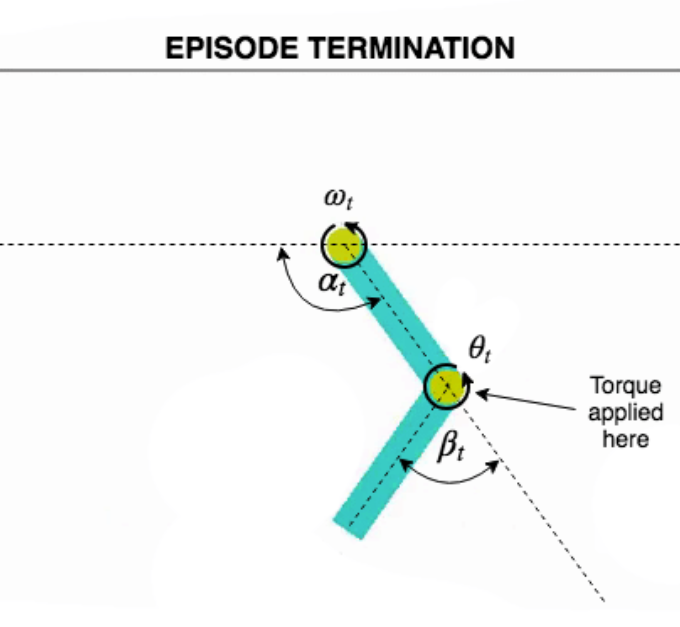
\includegraphics{thesis/images/acrobot_env.png}}}
    \caption{Trò chơi Acrobot}
    \label{fig:flappybird}
\end{figure}
Acrobot là một con lắc 2 liên kết chỉ có khớp thứ hai được kích hoạt. Ban đầu, cả hai liên kết đều hướng xuống dưới. Mục tiêu là để xoay bộ phận đầu cuối ở độ cao mà ít nhất là chiều dài của một liên kết nằm ở phía trên đường cơ sở. Cả hai liên kết có thể xoay tự do và có thể đi qua nhau, tức là, chúng không va chạm khi chúng có cùng một góc. Trò chơi bao gồm các trạng thái của môi trường là các hàm sin() và cos() của 2 khớp góc quay và vận tốc góc khớp đó là [$\cos(\theta_1)$, $\sin(\theta_1)$, $\cos(\theta_2)$, $\sin(\theta_2)$, $\Dot{\theta_1}$, $\Dot{\theta_2}$]. Đối với liên kết đầu tiên, một góc 0 tương ứng với liên kết hướng xuống dưới. Góc của liên kết thứ hai liên quan đến góc của liên kết thứ nhất. Một góc 0 tương ứng với việc có cùng một góc giữa hai liên kết. Trạng thái [1, 0, 1, 0, ..., ...] có nghĩa là cả hai liên kết đều hướng xuống dưới. Các g
hành động cung cấp là áp dụng mô-men +1, 0 hoặc -1 trên khớp nối giữa hai liên kết con lắc. 

Chiều dài của mỗi liên kết được khởi tạo ban đầu gọi là $l_1$, $l_2$, cấu hình mạng ANN được sử dụng để học là (6,8,1). Trong đồ án này sẽ định nghĩa các tác vụ dựa theo sự khác nhau về độ dài của liên kết thứ 2:
\begin{table} [H]
    \begin{center}
    \caption{Danh sách các tác vụ thực nghiệm bài toán Acrobot}
    \scalebox{0.9}{\begin{tabular}{|c|c|c|c|c|c|}
    \hline
    \multirow{1}{*}{\textbf{Tham số}} & \multicolumn{1}{c|}{\textbf{Tác vụ 1}} & \multicolumn{1}{c|}{\textbf{Tác vụ 2}} & \multicolumn{1}{c|}{\textbf{Tác vụ 3}} & \multicolumn{1}{c|}{\textbf{Tác vụ 4}} & \multicolumn{1}{c|}{\textbf{Tác vụ 5}} \\ \hline
    $l_2$ & $l_2=0.8$ & $l_2=0.9$ & $l_2=1.0$ & $l_2=1.1$ & $l_2=1.2$ \\\hline
    \end{tabular}}
    \end{center}
    \label{tab:result:flappybird}
\end{table}

\subsubsection{PixelCopter}
\begin{figure}[h!]
    \centering
    \scalebox{0.5}{\fbox{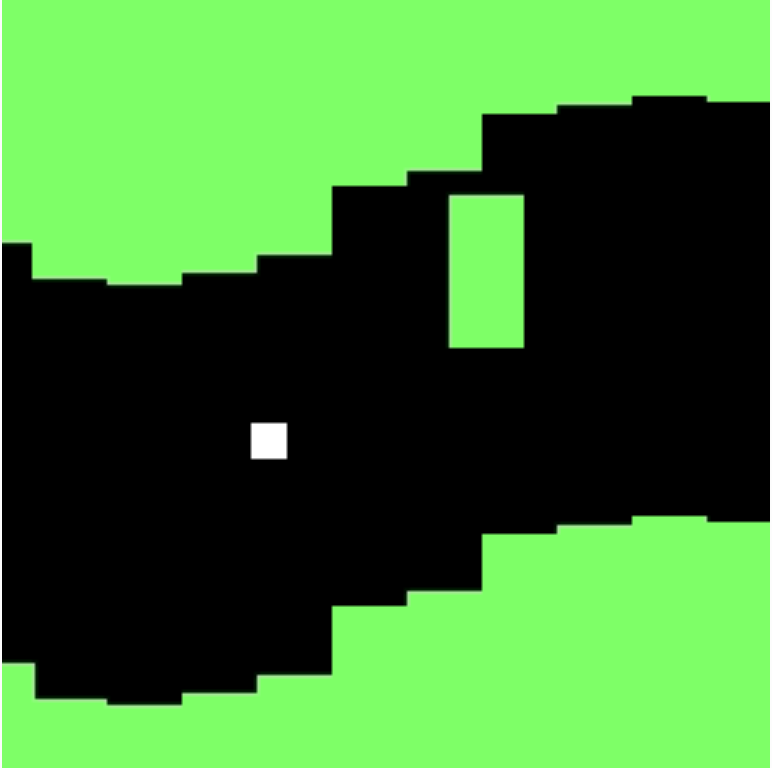
\includegraphics{thesis/images/pixelcopter.png}}}
    \caption{Trò chơi PixelCopter}
    \label{fig:flappybird}
\end{figure}
Pixelcopter là trò chơi đòi hỏi người chơi phải vượt qua các vật cản bên trong một hang động. Đây là bản sao chép của trò chơi máy bay trực thăng nổi tiếng (thuật ngữ gốc: \emph{helicopter}) với người chơi chỉ là một đơn vị pixel khiêm tốn. 
Với mỗi khối đơn vị chiều dài mà người chơi vượt qua sẽ nhận được một điểm thưởng là +1. Khi trò chơi kết thúc sẽ nhận được một điểm thưởng âm là -1. Trò chơi kết thúc khi người choi va đập vào thành hang, hoặc các chướng ngại vật trong hang. Trạng thái của trò chơi được biểu diễn bởi một véc-tơ 7 chiều mô tả vị trí của pixel và các vật cản ở gần. Để mô hình hóa policy của bài toán dưới dạng mạng ANN, đồ án sử dụng một mạng ANN có cấu trúc là (7,8,1) tương ứng với đầu vào, lớp ẩn, đầu ra của policy.

Trong môi trường của trò chơi có một tham số là momentum ảnh hưởng đến tốc độ, và vị trí sau mỗi hành động của pixel. Trong đồ án này sẽ định nghĩa các tác vụ dựa theo sự khác nhau về momentum giữa các môi trường:
\begin{table} [H]
    \begin{center}
    \caption{Danh sách các tác vụ thực nghiệm bài toán Pixelcopter}

    \scalebox{0.85}{\begin{tabular}{|c|c|c|c|c|c|}
    \hline
    \multirow{1}{*}{\textbf{Tham số}} & \multicolumn{1}{c|}{\textbf{Tác vụ 1}} & \multicolumn{1}{c|}{\textbf{Tác vụ 2}} & \multicolumn{1}{c|}{\textbf{Tác vụ 3}} & \multicolumn{1}{c|}{\textbf{Tác vụ 4}} & \multicolumn{1}{c|}{\textbf{Tác vụ 5}} \\ \hline
    momentum & $momentum=0$ & $momentum=0.1$ & $momentum=0.2$ & $momentum=0.3$ & $momentum=0.4$\\\hline
    \end{tabular}}
    \end{center}
    \label{tab:result:flappybird}
\end{table}

\subsubsection{FlappyBird}
\begin{figure}[h!]
    \centering
    \scalebox{0.5}{\fbox{
\includegraphics{flappy-bird_tbqj.jpg}}}
    \caption{Trò chơi FlappyBird}
    \label{fig:flappybird}
\end{figure}
Là trò chơi mà ở đó tác nhân (chú chim) phải vượt qua được khoảng trống giữa các ống. Trong trò chơi tác nhân chỉ thực hiện 2 hành động: hướng lên, hướng xuống. Mũi tên hướng lên khiến chim trong trò chơi sẽ đi lên, mũi trên hướng xuống khiến chim đi xuống. Trong trường hợp chim đập xuống đất, đập vào thành ống hoặc đập lên phía trên màn hình thì trò chơi sẽ kết thúc. Mỗi lượt chim qua một ống sẽ được tính là được thêm $+1$ điểm thưởng. Mỗi lần tới trạng thái kết thúc sẽ nhận được một điểm thưởng âm là $-1$. Có 8 trạng thái biểu diễn vị trí 2D của chim, vị trí của vật cản tiếp theo, vị trị của vật cản tiếp theo sau đó. Với bài toán này trong đồ án sẽ sử dụng một mạng ANN có cấu hình là $(8,4,1)$ tương ứng với đầu vào, lớp ẩn, đầu ra của mạng để có thể học được mô hình policy của bài toán.

Trong môi trường của trò chơi có một tham số là trọng lực (thuật ngữ gốc: \emph{gravity}. Trong đồ án này sẽ định nghĩa các tác vụ dựa theo sự khác nhau về trọng lực giữa các môi trường:
\begin{table} [H]
    \begin{center}
    \caption{Danh sách các tác vụ thực nghiệm bài toán FlappyBird}

    \scalebox{0.9}{\begin{tabular}{|c|c|c|c|c|c|}
    \hline
    \multirow{1}{*}{\textbf{Tham số}} & \multicolumn{1}{c|}{\textbf{Tác vụ 1}} & \multicolumn{1}{c|}{\textbf{Tác vụ 2}} & \multicolumn{1}{c|}{\textbf{Tác vụ 3}} & \multicolumn{1}{c|}{\textbf{Tác vụ 4}} & \multicolumn{1}{c|}{\textbf{Tác vụ 5}} \\ \hline
    gravity & $gravity=0.8$ & $gravity=1.8$ & $gravity=2.8$ & $gravity=3.8$ & $gravity=4.8$\\\hline
    \end{tabular}}
    \end{center}
    \label{tab:result:flappybird}
\end{table}

\section{Cài đặt thực nghiệm}
Các thực nghiệm được triển khai hoàn toàn trên hệ thống Ubuntu 18.04 LTS 64-bit với mô tả cấu hình như phía dưới:
\begin{itemize}
    \item CPU: Intel\textregistered Core\texttrademark i5-2430M CPU @ 2.40GHz × 2
    \item RAM: 6GB
    \item Ngôn ngữ lập trình: Python 3.6
    \item Mã nguồn: https://github.com/minhquang4334/mfeaii-ann-rl
\end{itemize}

\subsection{Cấu hình cho bài toán huấn luyện các mạng neural khác cấu trúc}
Các thuật toán đều chạy trên mỗi cấu hình thực nghiệm 30 lần. Độ đo hiệu quả giải thuật là MSE được thống kê trên cả bộ dữ liệu học và bộ dữ liệu kiểm định. Độ đo được thống kê trong 30 lần chạy để so sánh kết quả trung bình cùng độ lệch chuẩn.
\begin{table}[h!]
    \centering
    \caption{Cấu hình và tham số giải thuật đề xuất cho bài toán huấn luyện các mạng neural khác cấu trúc}

	\begin{tabular}{|l|c|c|c|c|}
        \hline
        \multirow{1}{*}{\textbf{Tham số}} & 
        \multicolumn{1}{c|} {\textbf{Ký hiệu}} & \multicolumn{1}{c|}{\textbf{Giá trị}}\\ \hline
        Kích thước quần thể đơn nhiệm & $N_k$ & 30\\
        Số tác vụ & $K$ & 3\\
        Kích thước quần thể đa nhiệm & $N$ & $N_k \cdot K$\\
        Số thế hệ tiến hóa & $T$ & 1000\\
        Chỉ số phân phối SBX & $\eta_c$ & 15\\
        Tỉ lệ đột biến PMU & $\sigma$ & 0.2\\
        Chỉ số đột biến PMU & $\eta_m$ & 15\\
        % pswap & - & 0.5\\
        Giá trị tham số cố định $rmp$ của thuật toán $MFEA$ & $rmp$ & 0.5\\
        Giá trị khởi tạo các phần tử trong ma trận $RMP$ & $rmp_{k,j}$ & 0\\
        Giá trị chặn dưới của từng phần tử $rmp_{kj}, k,j \in {K}$  & - & 0.1\\
        Số lần chạy thống kê & - & 30\\ \hline
    \end{tabular}
    \label{tab:config:nbit}
\end{table}
\subsection{Cấu hình cho bài toán huấn luyện nhiều mô hình học tăng cường}
Các thuật toán đều chạy trên mỗi cấu hình thực nghiệm 30 lần. Độ đo hiệu quả giải thuật là tổng phần thưởng thu được với bộ tham số hiện tại. Độ đo được thống kê trong 30 lần chạy để so sánh kết quả trung bình cùng độ lệch chuẩn.
\begin{table}[h!]
    \centering
    \caption{Cấu hình và tham số giải thuật đề xuất cho bài toán huấn luyện nhiều mô hình học tăng cường}

    \begin{tabular}{|l|c|c|c|c|}
        \hline
        \multirow{1}{*}{\textbf{Tham số}} & 
        \multicolumn{1}{c|} {\textbf{Ký hiệu}} & \multicolumn{1}{c|}{\textbf{Giá trị}}\\ \hline
        Kích thước quần thể đơn nhiệm & $N_k$ & 30\\
        Số tác vụ & $K$ & 5\\
        Kích thước quần thể đa nhiệm & $N$ & $N_k \cdot K$\\
        Số thế hệ tiến hóa & $T$ & 200\\
        Chỉ số phân phối SBX & $\eta_c$ & 15\\
        Tỉ lệ đột biến PMU & $\sigma$ & 0.2\\
        Chỉ số đột biến PMU & $\eta_m$ & 15\\
        % pswap & - & 0.5\\
        Giá trị tham số cố định $rmp$ của thuật toán $MFEA$ & $rmp$ & 0.5\\
        Giá trị khởi tạo các phần tử trong ma trận $RMP$ & $rmp_{k,j}$ & 0\\
        Giá trị chặn dưới của từng phần tử $rmp_{kj}, k,j \in {K}$  & - & 0.1\\
        Số lần chạy thống kê & - & 30\\ \hline
        
    \end{tabular}
    \label{tab:config:rl}
\end{table}


\section{Kết quả}

\subsection{Huấn luyện nhiều mô mạng neural đa lớp}
\subsubsection{Bảng kết quả thực nghiệm - mạng neural cùng độ sâu 1 lớp ẩn}

\begin{table} [H]
    \begin{center}
        \caption{Kết quả thực nghiệm bài 4-bit 1 lớp ẩn}

    \begin{tabular}{|c|c|c|c|}
    \hline
    \multirow{1}{*}{\textbf{Method}} & \multicolumn{1}{c|}{\textbf{Subtask1}} & \multicolumn{1}{c|}{\textbf{Subtask 2}} & \multicolumn{1}{c|}{\textbf{Subtask 3}} \\ \hline
    CEA & $0.0316 \pm 0.0125$ & $0.0201 \pm 0.011922$ & $0.0117 \pm 0.008133$ \\
    MFEA-I & $0.025 \pm 0.012957$ & $0.0117 \pm 0.007342$ & $0.0072 \pm 0.005355$\\
    MFEA-II  & $\mathbf{0.0219 \pm 0.009181}$ & $\mathbf{0.0099 \pm 0.007053}$ & $\mathbf{0.0052 \pm 0.004126}$ \\\hline
    
    \end{tabular}
    \end{center}
    
    \label{tab:result:nbit}
\end{table}
\begin{table} [H]   
    \begin{center}
        \caption{Kết quả thực nghiệm bài 6-bit 1 lớp ẩn}

    \begin{tabular}{|c|c|c|c|}
    \hline
    \multirow{1}{*}{\textbf{Method}} & \multicolumn{1}{c|}{\textbf{Subtask1}} & \multicolumn{1}{c|}{\textbf{Subtask 2}} & \multicolumn{1}{c|}{\textbf{Subtask 3}} \\ \hline
    CEA(5,6,7)  & $0.0703 \pm 0.014543$ & $0.0619 \pm 0.018078$ & $0.0572 \pm 0.017982$ \\
    MFEA-I(5,6,7)   & $\mathbf{0.06 \pm 0.014702}$ & $\mathbf{0.0498 \pm 0.009562}$ & $0.047 \pm 0.008464$ \\
    MFEA-II(5,6,7)  & $0.06 \pm 0.011387$ & $0.052 \pm 0.009393$ & $\mathbf{0.047 \pm 0.009579}$ \\\hline
    
    CEA(6,7,8)   & $0.0669 \pm 0.016032$ & $0.0583 \pm 0.009948$ & $0.0521 \pm 0.015598$ \\
    MFEA-I(6,7,8)  & $0.0611 \pm 0.013622$ & $0.0528 \pm 0.011122$ & $0.0484 \pm 0.011074$ \\
    MFEA-II(6,7,8) & $\mathbf{0.0522 \pm 0.011066}$ & $\mathbf{0.0476 \pm 0.01033}$ & $\mathbf{0.0418 \pm 0.011741}$ \\\hline
    
    \end{tabular}
    \end{center}
    \label{tab:result:nbit}
\end{table}    
\begin{table} [H]
    \begin{center}
        \caption{Kết quả thực nghiệm bài 8-bit 1 lớp ẩn}

    \begin{tabular}{|c|c|c|c|}
    \hline
    \multirow{1}{*}{\textbf{Method}} & \multicolumn{1}{c|}{\textbf{Subtask1}} & \multicolumn{1}{c|}{\textbf{Subtask 2}} & \multicolumn{1}{c|}{\textbf{Subtask 3}} \\ \hline
    CEA(5,6,7) & $0.0956 \pm 0.013764$ & $0.0906 \pm 0.015274$ & $0.0874 \pm 0.010884$ \\
    MFEA-I(5,6,7) & $0.0859 \pm 0.011722$ & $0.0801 \pm 0.009489$ & $0.0778 \pm 0.010507$  \\
    MFEA-II(5,6,7) & $\mathbf{0.0827 \pm 0.010678}$ & $\mathbf{0.076 \pm 0.012979}$ & $\mathbf{0.0735 \pm 0.012598}$ \\\hline
    
    CEA(6,7,8)& $0.0895 \pm 0.012499$ & $0.0902 \pm 0.013171$ & $0.081 \pm 0.013371$ \\
    MFEA-I(6,7,8)  & $0.0826 \pm 0.011089$ & $0.0768 \pm 0.010228$ & $0.0734 \pm 0.008805$ \\
    MFEA-II(6,7,8) & $\mathbf{0.0808 \pm 0.010726}$ & $\mathbf{0.0739 \pm 0.01117}$ & $\mathbf{0.072 \pm 0.009657}$ \\\hline
    \end{tabular}
    \end{center}
    \label{tab:result:nbit}
\end{table}

\subsubsection{Biểu đồ hội tụ - mạng neural cùng độ sâu 1 lớp ẩn}
\begin{figure}[H]
    \centering

    \scalebox{.7}{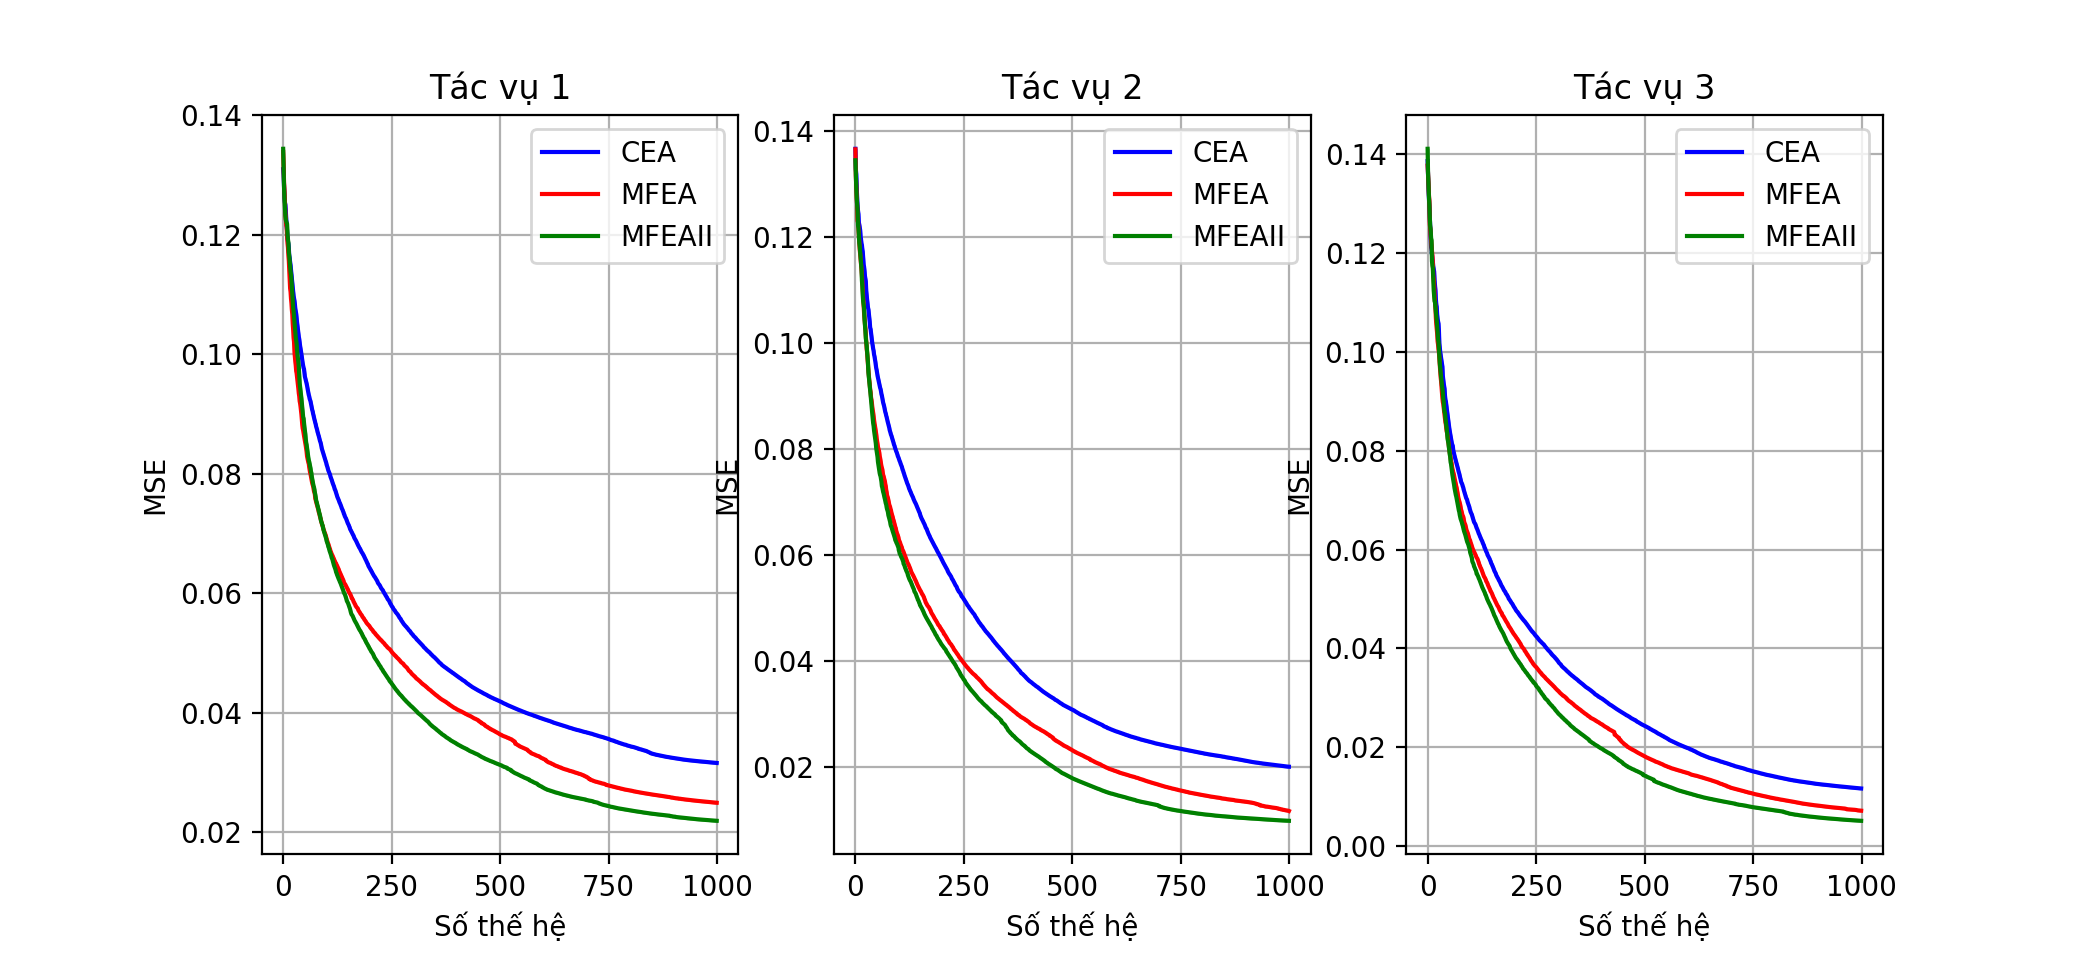
\includegraphics[width=\textwidth,height=\textheight,keepaspectratio]{thesis/images/results/nbit_1layer/4bit_task.png}}
    \scalebox{.7}{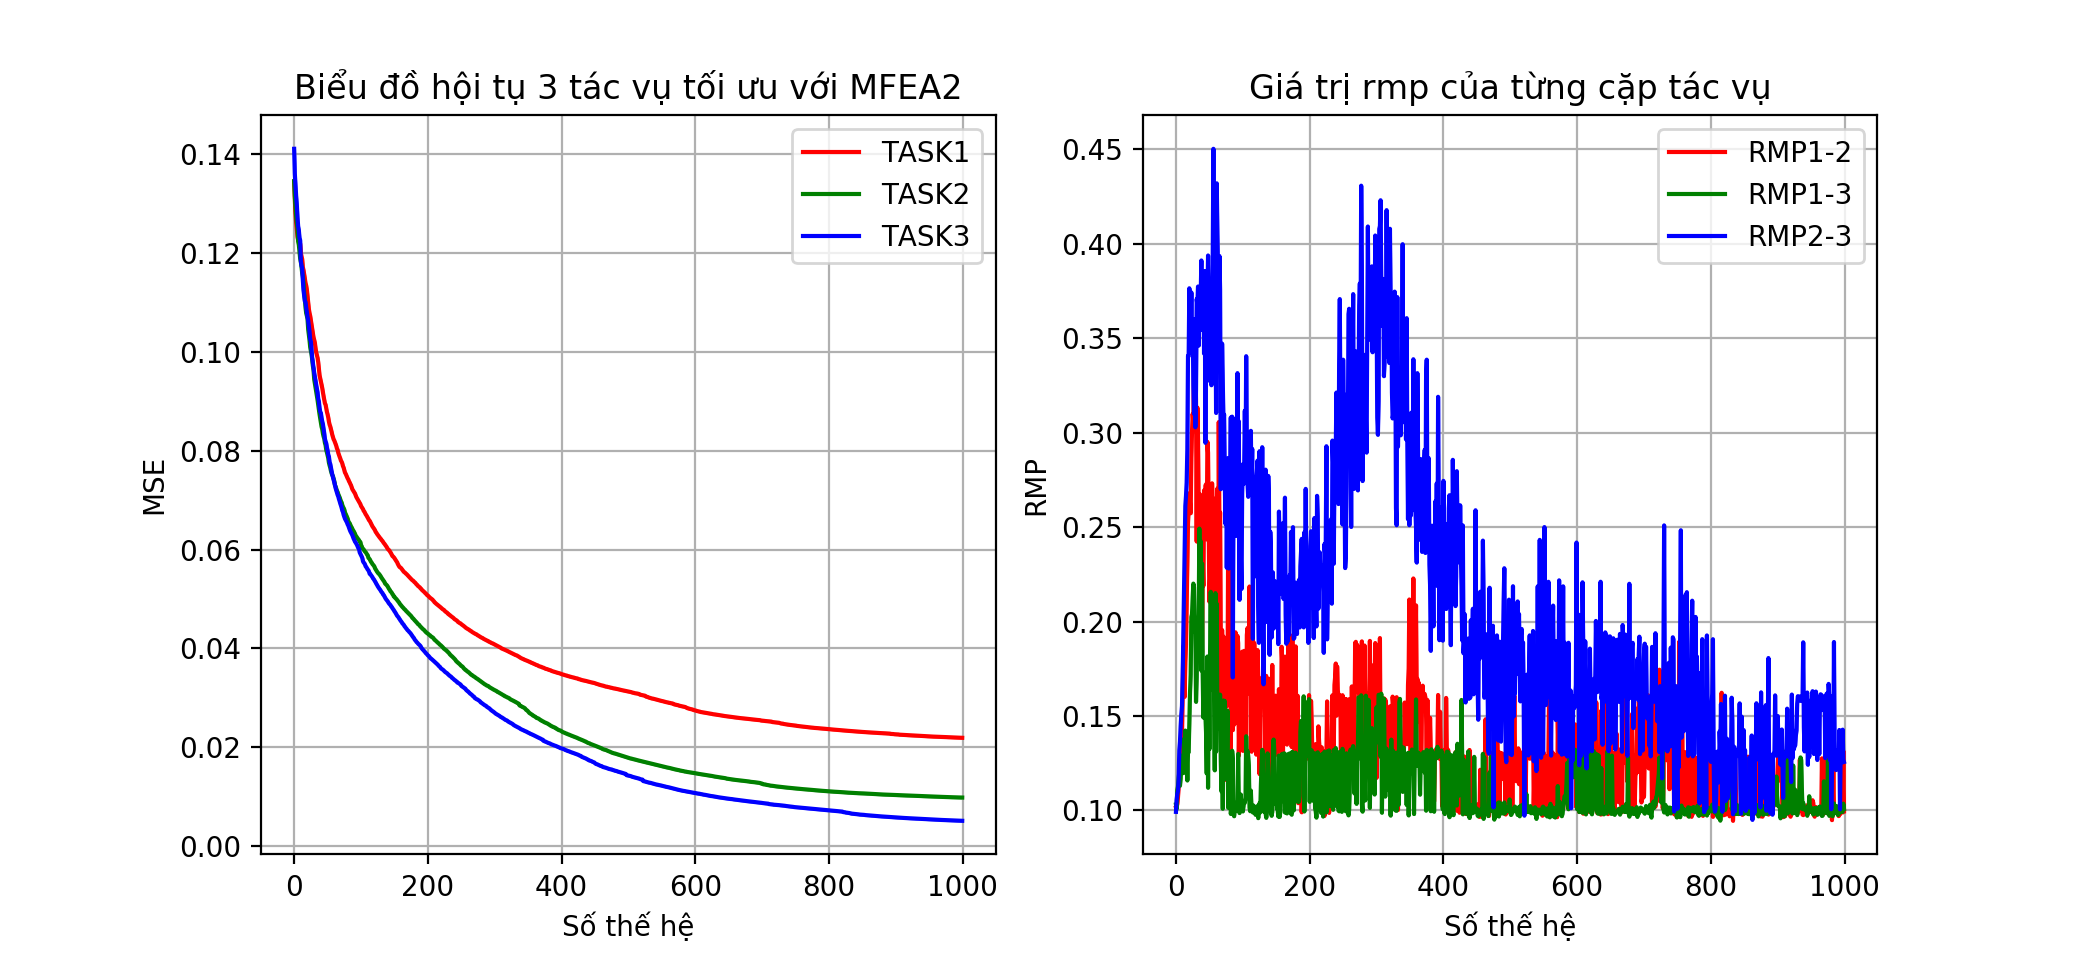
\includegraphics[width=\textwidth,height=\textheight,keepaspectratio]{thesis/images/results/nbit_1layer/4bit_rmp.png}}
    \label{fig:4bit_1layer}
    \caption{Bài 4bit: Biểu đồ hội tụ của từng tác vụ trên các thuật toán và biểu đồ phân tích MFEA-II theo giá trị rmp}

\end{figure}
\begin{figure}[H]
    \centering
    \scalebox{.7}{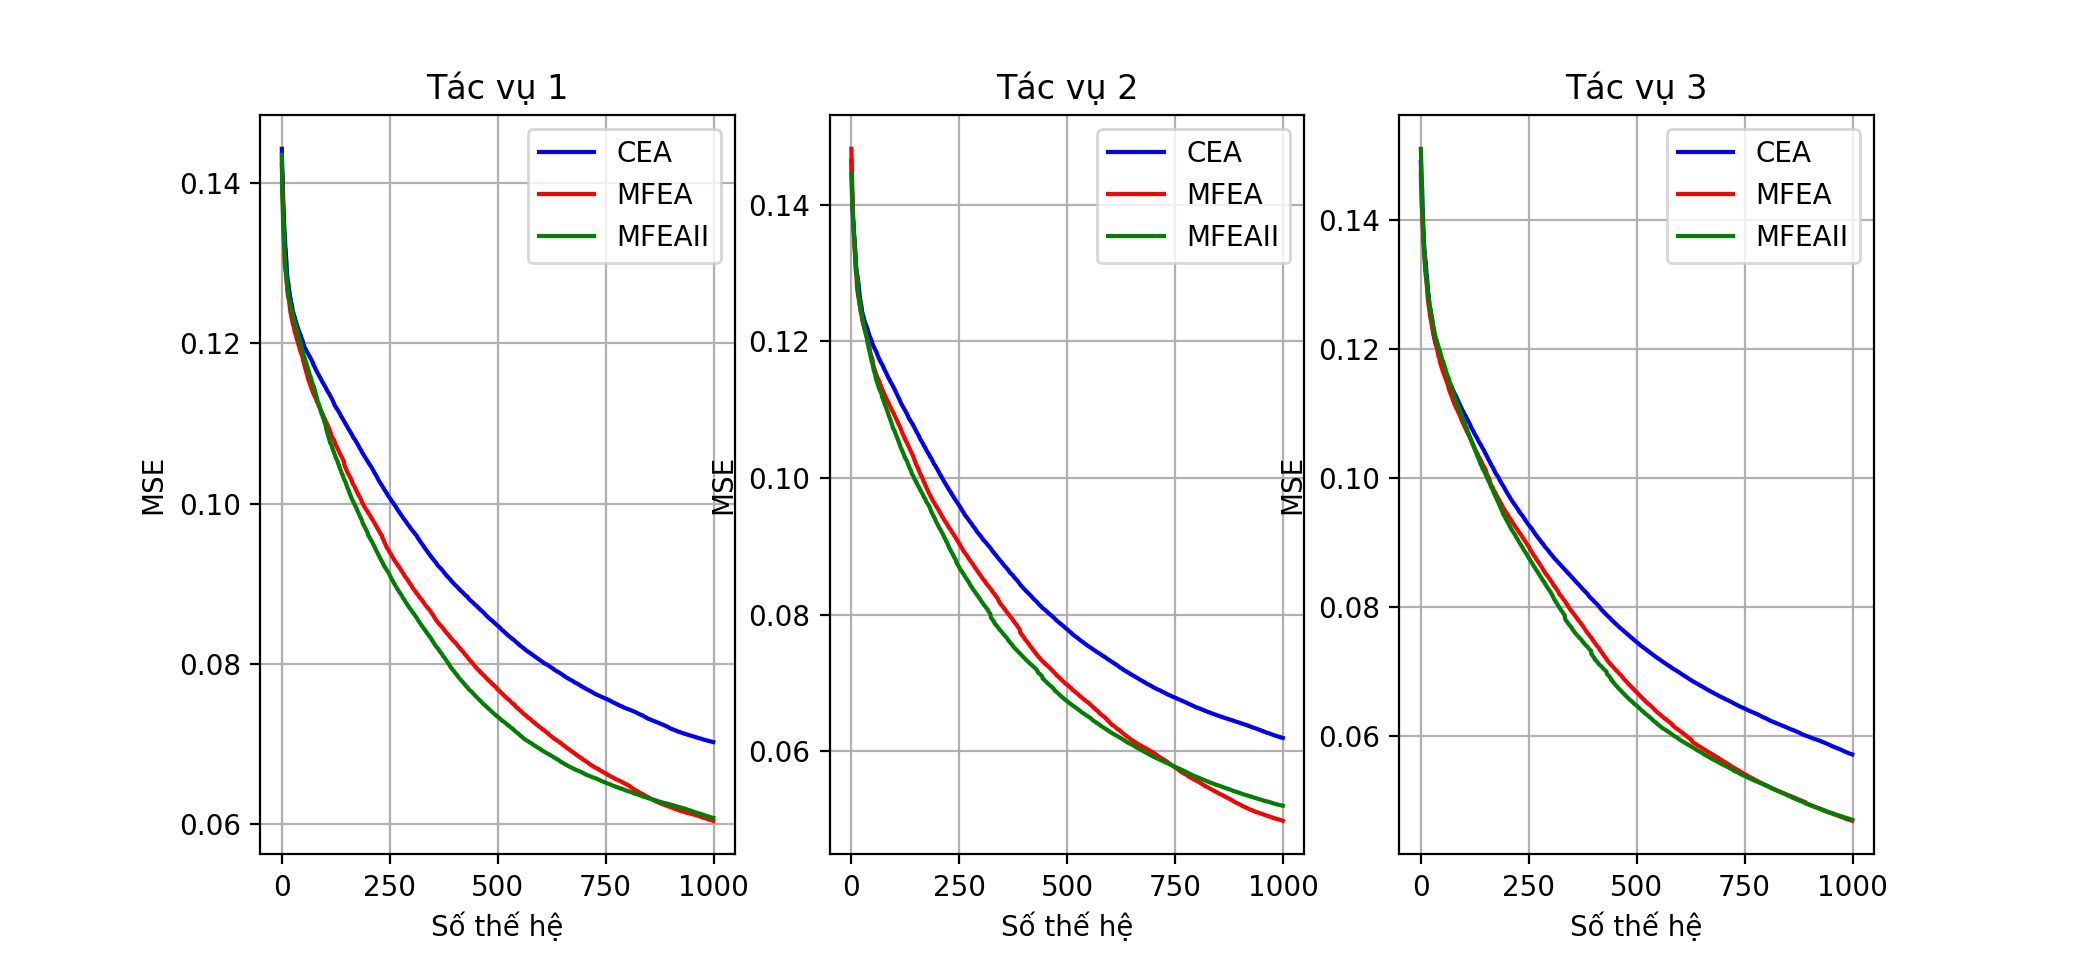
\includegraphics[width=\textwidth,height=\textheight,keepaspectratio]{thesis/images/results/nbit_1layer/6bit1_task.png}}
    \scalebox{.7}{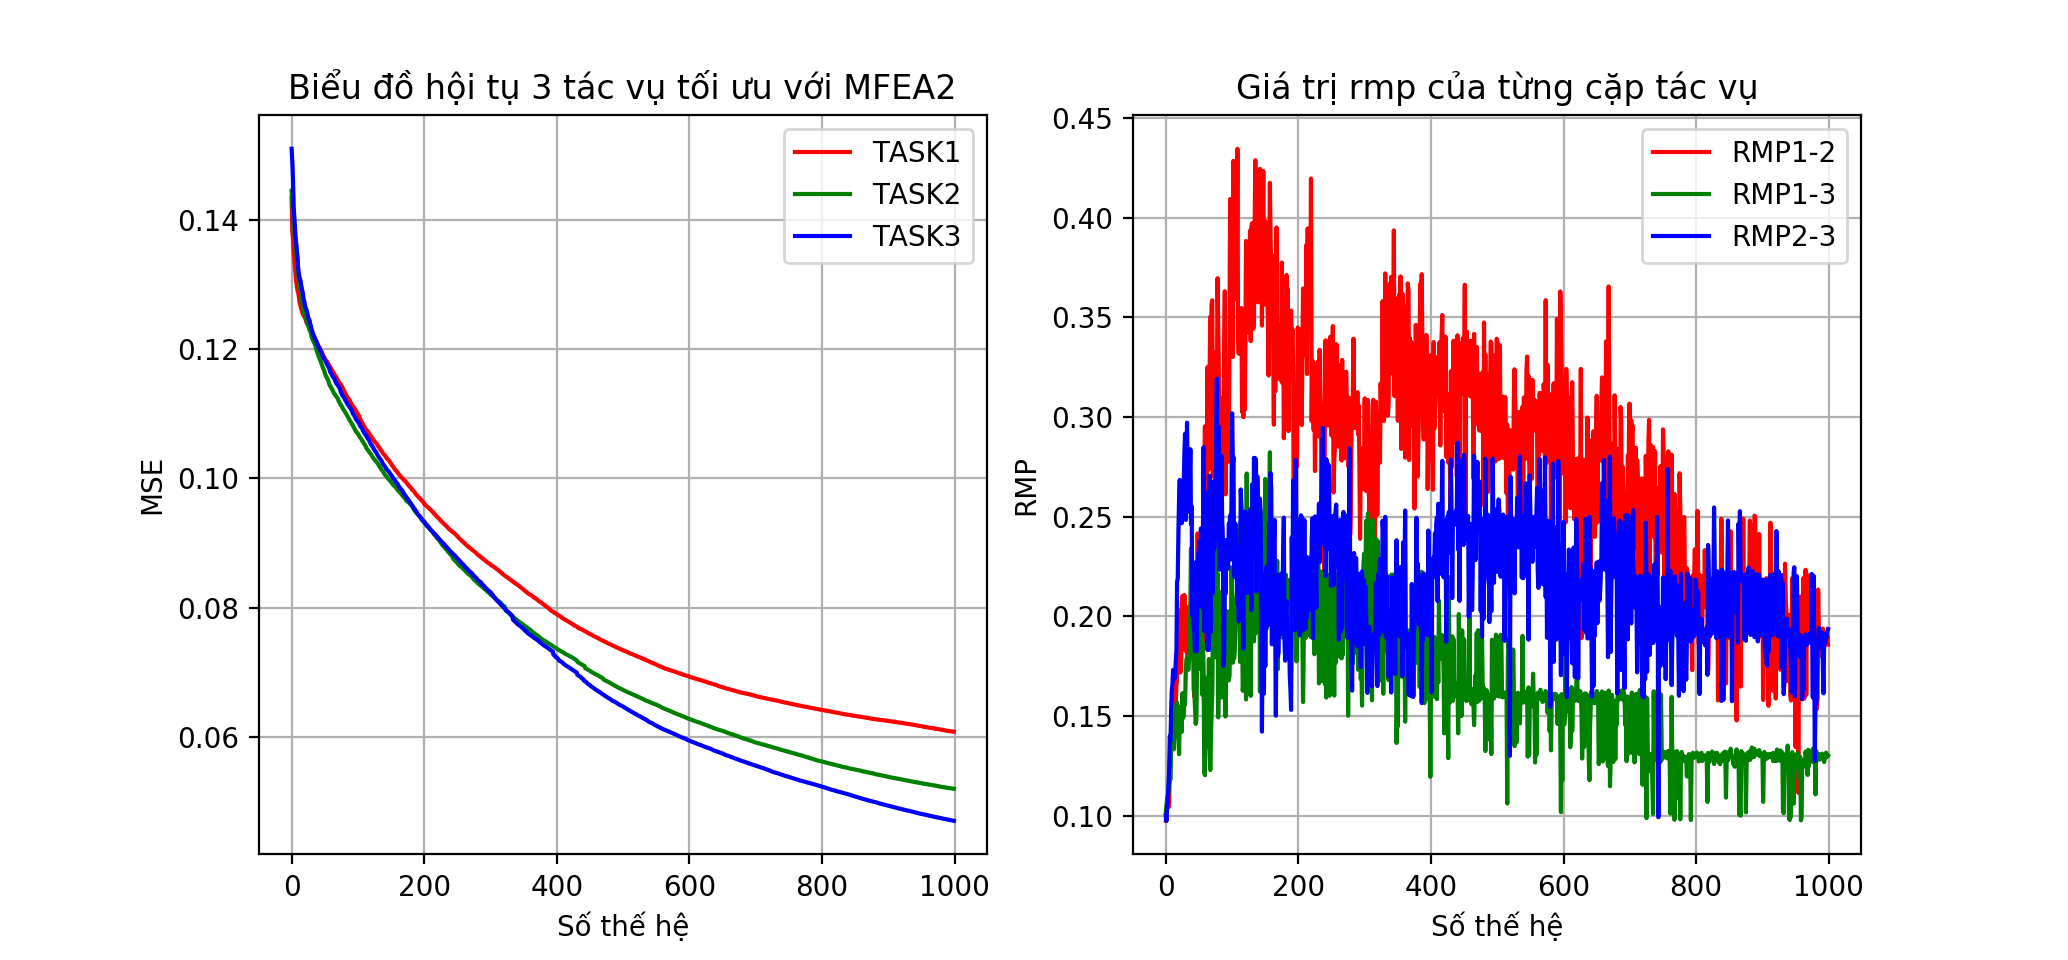
\includegraphics[width=\textwidth,height=\textheight,keepaspectratio]{thesis/images/results/nbit_1layer/6bit1_rmp.png}}
    \label{fig:6bit_1}
    \caption{Bài 6bit(5,6,7): Biểu đồ hội tụ của từng tác vụ trên các thuật toán và biểu đồ phân tích MFEA-II theo giá trị rmp}

\end{figure}
\begin{figure}[H]

    \centering
    \scalebox{.7}{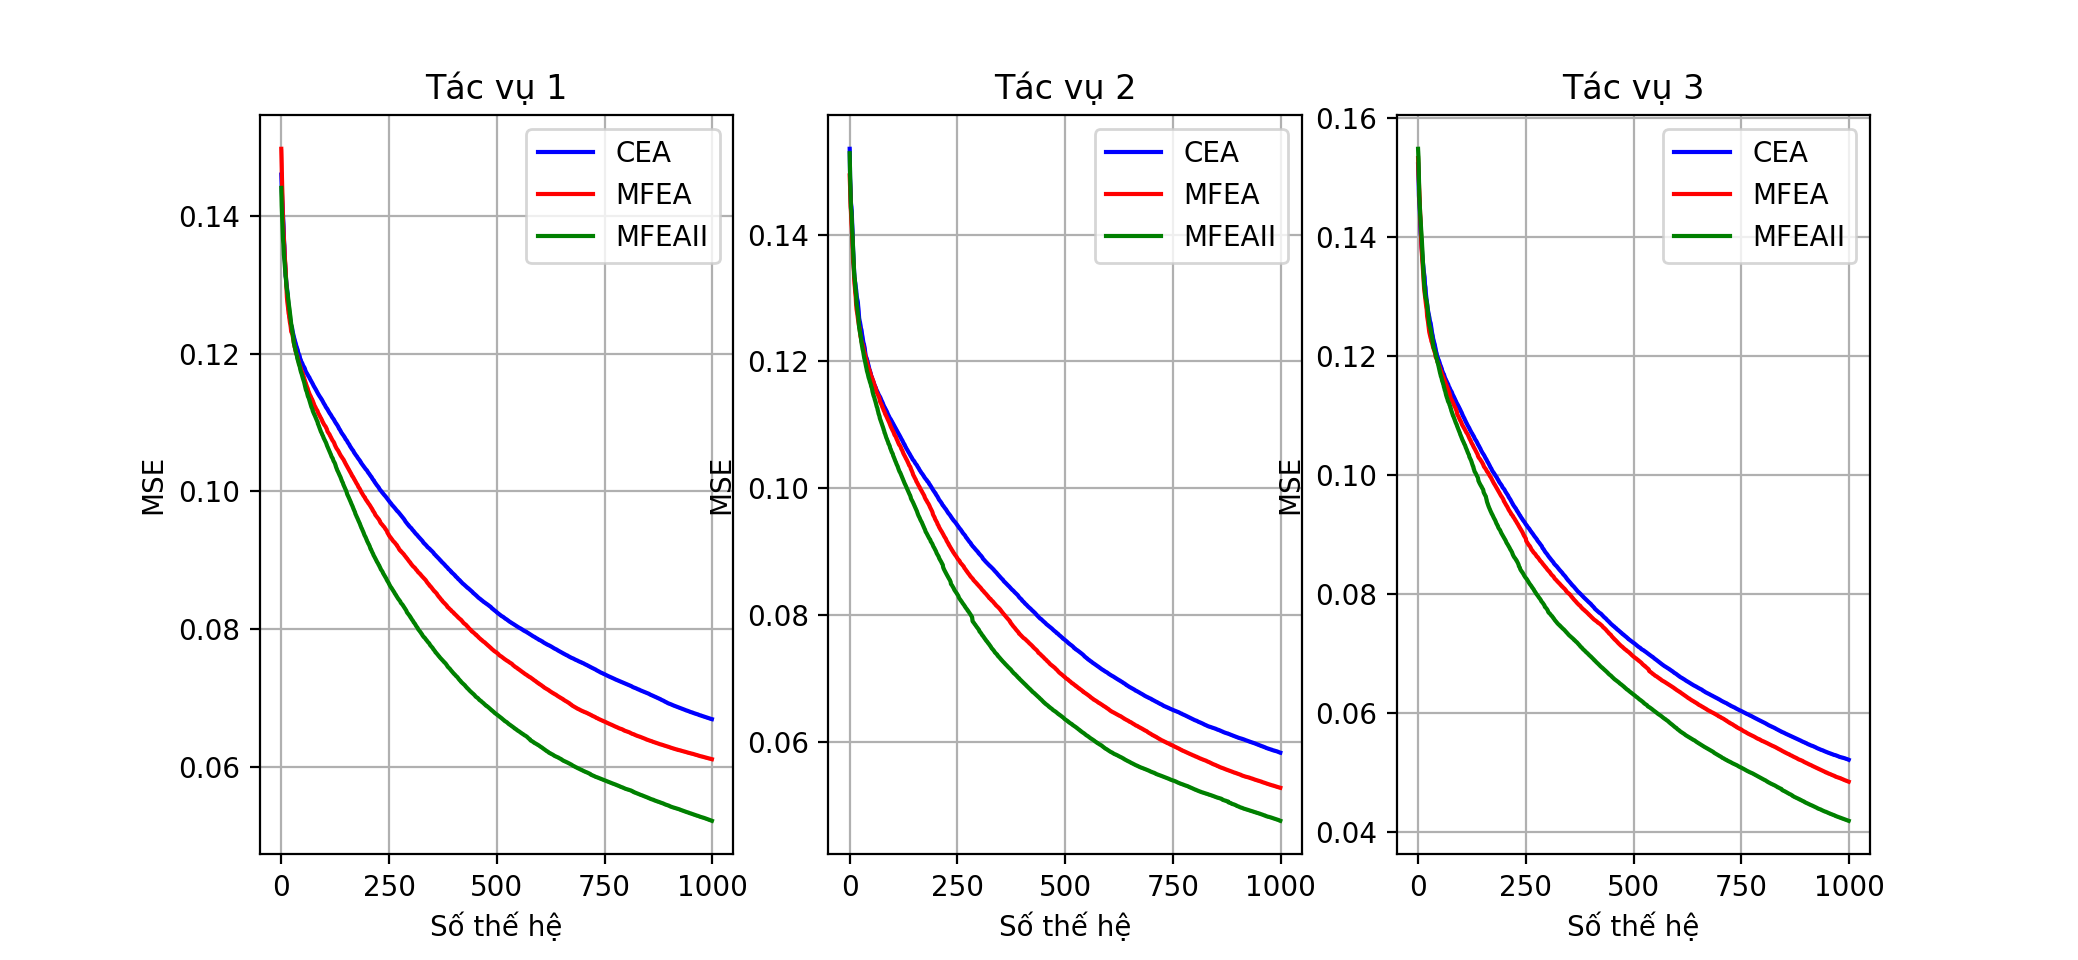
\includegraphics[width=\textwidth,height=\textheight,keepaspectratio]{thesis/images/results/nbit_1layer/6bit2_task.png}}
    \scalebox{.7}{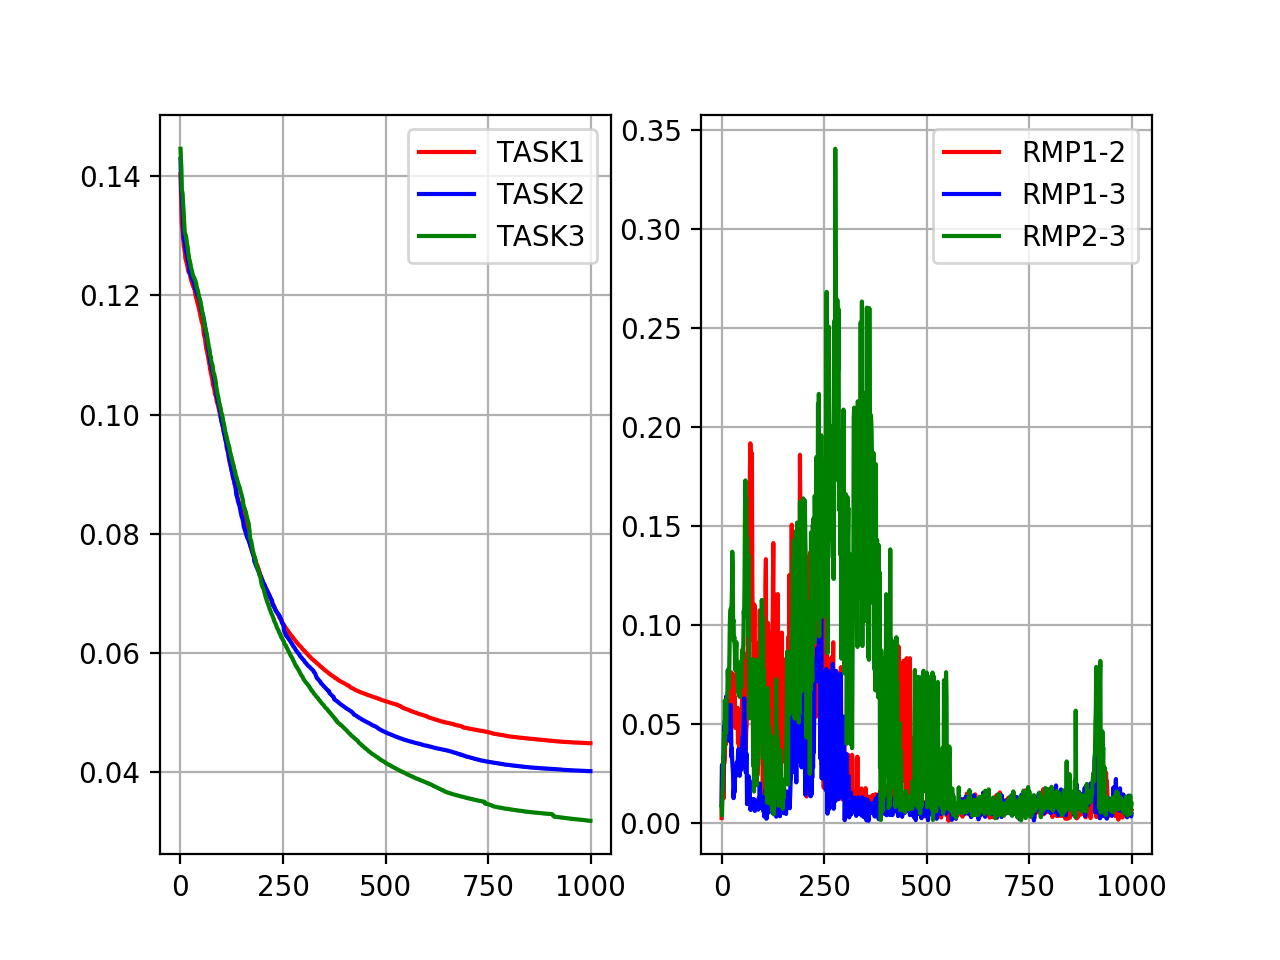
\includegraphics[width=\textwidth,height=\textheight,keepaspectratio]{thesis/images/results/nbit_1layer/6bit2_rmp.png}}
    \label{fig:6bit2_1layer}
        \caption{Bài 6bit(6,7,8): Biểu đồ hội tụ của từng tác vụ trên các thuật toán và biểu đồ phân tích MFEA-II theo giá trị rmp}

\end{figure}
\begin{figure}[H]
    \centering

    \scalebox{.7}{\includegraphics[width=\textwidth,height=\textheight,keepaspectratio]{thesis/images/results/nbit_1layer/8bit1_task.png}}
    \scalebox{.7}{\includegraphics[width=\textwidth,height=\textheight,keepaspectratio]{thesis/images/results/nbit_1layer/8bit1_rmp.png}}
    \label{fig:8bit1_1layer}
    \caption{Bài 8bit(5,6,7):Biểu đồ hội tụ của từng tác vụ trên các thuật toán và biểu đồ phân tích MFEA-II theo giá trị rmp}

\end{figure}
\begin{figure}[H]
    \centering

    \scalebox{.7}{\includegraphics[width=\textwidth,height=\textheight,keepaspectratio]{thesis/images/results/nbit_1layer/8bit2_task.png}}
    \scalebox{.7}{\includegraphics[width=\textwidth,height=\textheight,keepaspectratio]{thesis/images/results/nbit_1layer/8bit2_rmp.png}}
    \label{fig:8bit2_1layer}
    \caption{Bài 8bit(6,7,8): Biểu đồ hội tụ của từng tác vụ trên các thuật toán và biểu đồ phân tích MFEA-II theo giá trị rmp}

\end{figure}

\subsubsection{Bảng kết quả thực nghiệm - mạng neural cùng độ sâu 2 lớp ẩn}
\begin{table} [H]
    \begin{center}
    \caption{Kết quả thực nghiệm huấn luyện ANN 2 lớp ẩn}
    \begin{tabular}{|c|c|c|c|c|}
    \hline
    \multirow{1}{*}{\textbf{Bài toán}} &
    \multirow{1}{*}{\textbf{Method}} & \multicolumn{1}{c|}{\textbf{Tác vụ 1}} & \multicolumn{1}{c|}{\textbf{Tác vụ 2}} & \multicolumn{1}{c|}{\textbf{Tác vụ 3}} \\ \hline
    \multirow{3}{*} 
    {8-bit} &
    CEA & $0.075 \pm 0.012865$ & $0.0713 \pm 0.013116$ & $0.0718 \pm 0.012432$  \\
    & MFEA-I & $0.0738 \pm 0.012508$ & $0.0684 \pm 0.013252$ & $0.0669 \pm 0.015076$   \\
    & MFEA-II & $\mathbf{0.0705 \pm 0.012856}$ & $\mathbf{0.0624 \pm 0.011079}$ & $\mathbf{0.0595 \pm 0.011252}$\\\hline
    \multirow{3}{*} 
    {9-bit} &
    CEA & $0.0826 \pm 0.010588$ & $0.0751 \pm 0.014406$ & $0.0785 \pm 0.010766$  \\
    & MFEA-I & $0.0827 \pm 0.010438$ & $0.0762 \pm 0.009495$ & $0.0737 \pm 0.009766$ \\
    & MFEA-II & $\mathbf{0.0795 \pm 0.012865}$ & $\mathbf{0.0705 \pm 0.009581}$ & $\mathbf{0.0685 \pm 0.011156}$ \\\hline
    \multirow{3}{*} 
    {10-bit} &
    CEA & $0.0853 \pm 0.01105$ & $0.0862 \pm 0.008326$ & $0.0856 \pm 0.008919$  \\
    & MFEA-I  & $0.0855 \pm 0.012229$ & $\mathbf{0.0782 \pm 0.009659}$ & $\mathbf{0.0752 \pm 0.009681}$ \\
    & MFEA-II & $\mathbf{0.0833 \pm 0.010222}$ & $0.0791 \pm 0.009846$ & $0.0762 \pm 0.010419$ \\\hline
    \end{tabular}
    \end{center}

    \label{tab:result:nbit}
\end{table}

\subsubsection{Biểu đồ hội tụ - Mạng neural cùng độ sâu 2 lớp ẩn}
\begin{figure}[h!]
    \centering
    \scalebox{.7}{\includegraphics[width=\textwidth,height=\textheight,keepaspectratio]{thesis/images/results/nbit_2layer/8bit1_task.png}}
    \scalebox{.7}{\includegraphics[width=\textwidth,height=\textheight,keepaspectratio]{thesis/images/results/nbit_2layer/8bit1_rmp.png}}
    \caption{Bài 8bit: Biểu đồ hội tụ của từng tác vụ trên các thuật toán và biểu đồ phân tích MFEA-II theo giá trị rmp}
    \label{fig:8bit_2layer}
\end{figure}
\begin{figure}[h!]
    \centering
    \scalebox{.7}{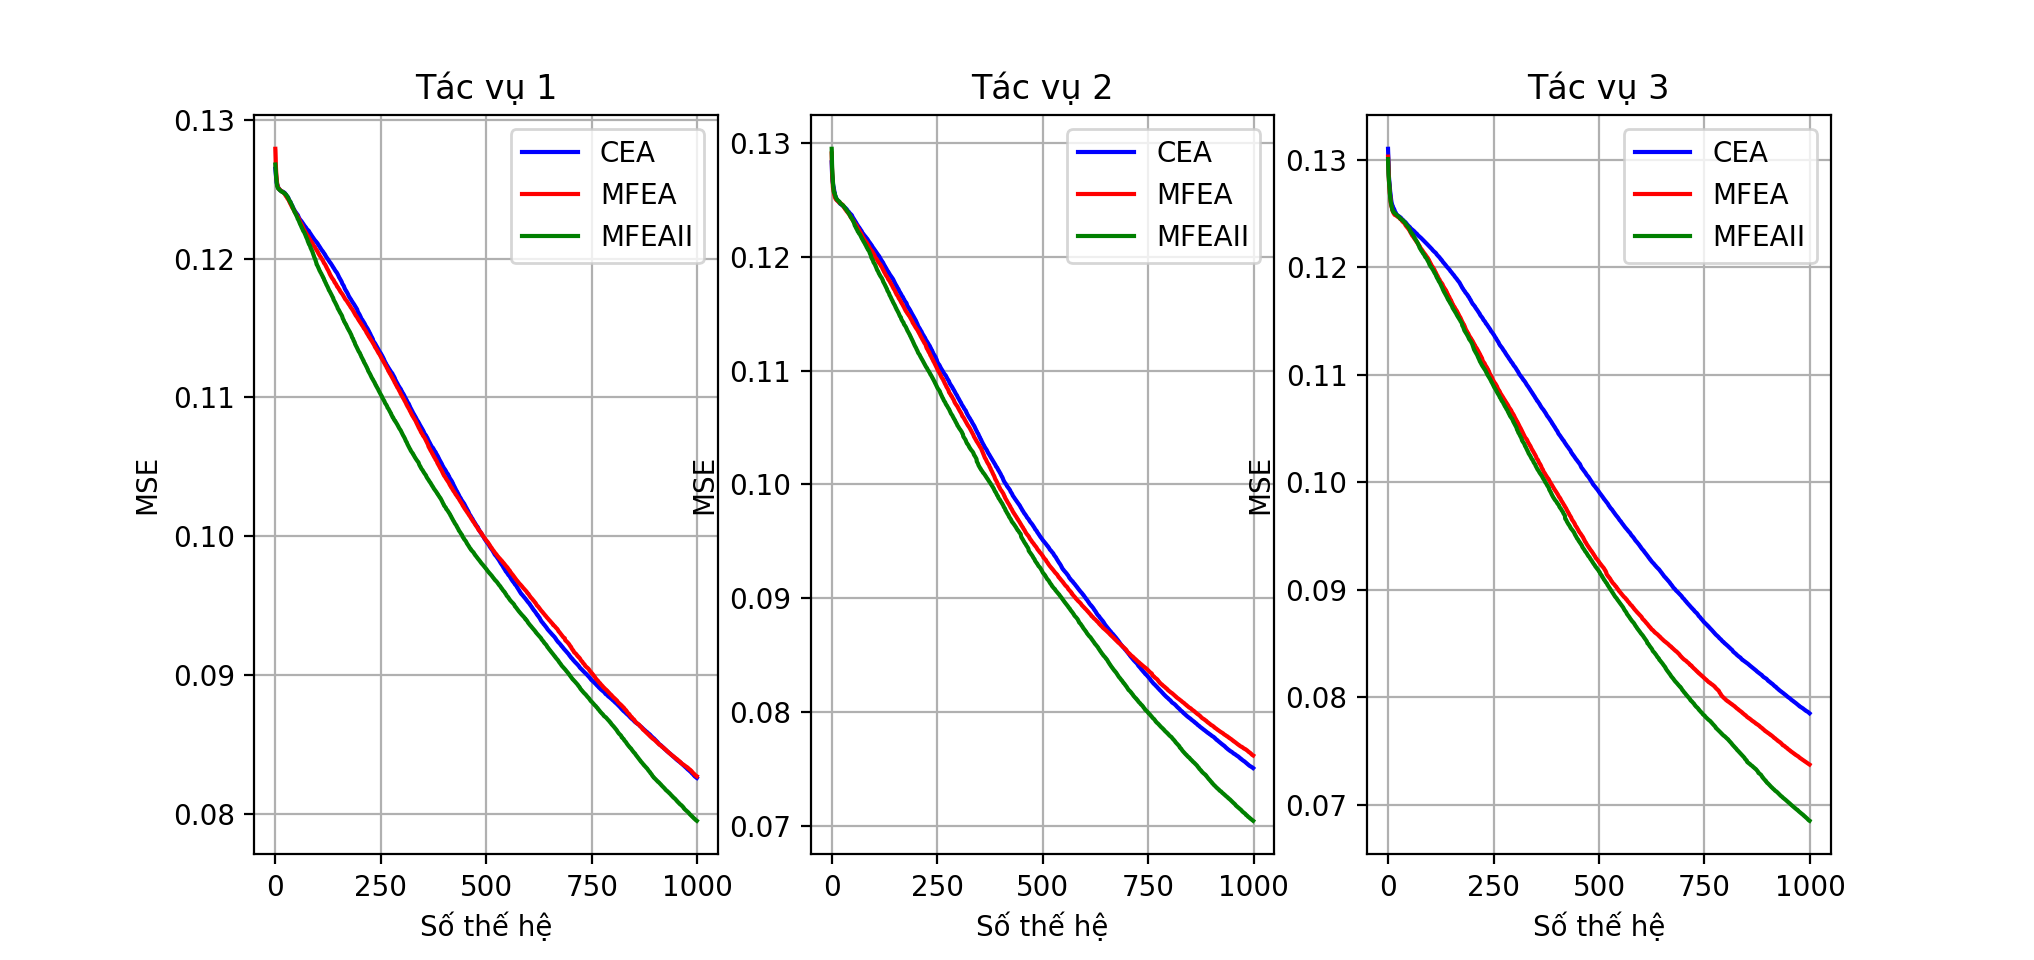
\includegraphics[width=\textwidth,height=\textheight,keepaspectratio]{thesis/images/results/nbit_2layer/9bit1_task.png}}
    \scalebox{.7}{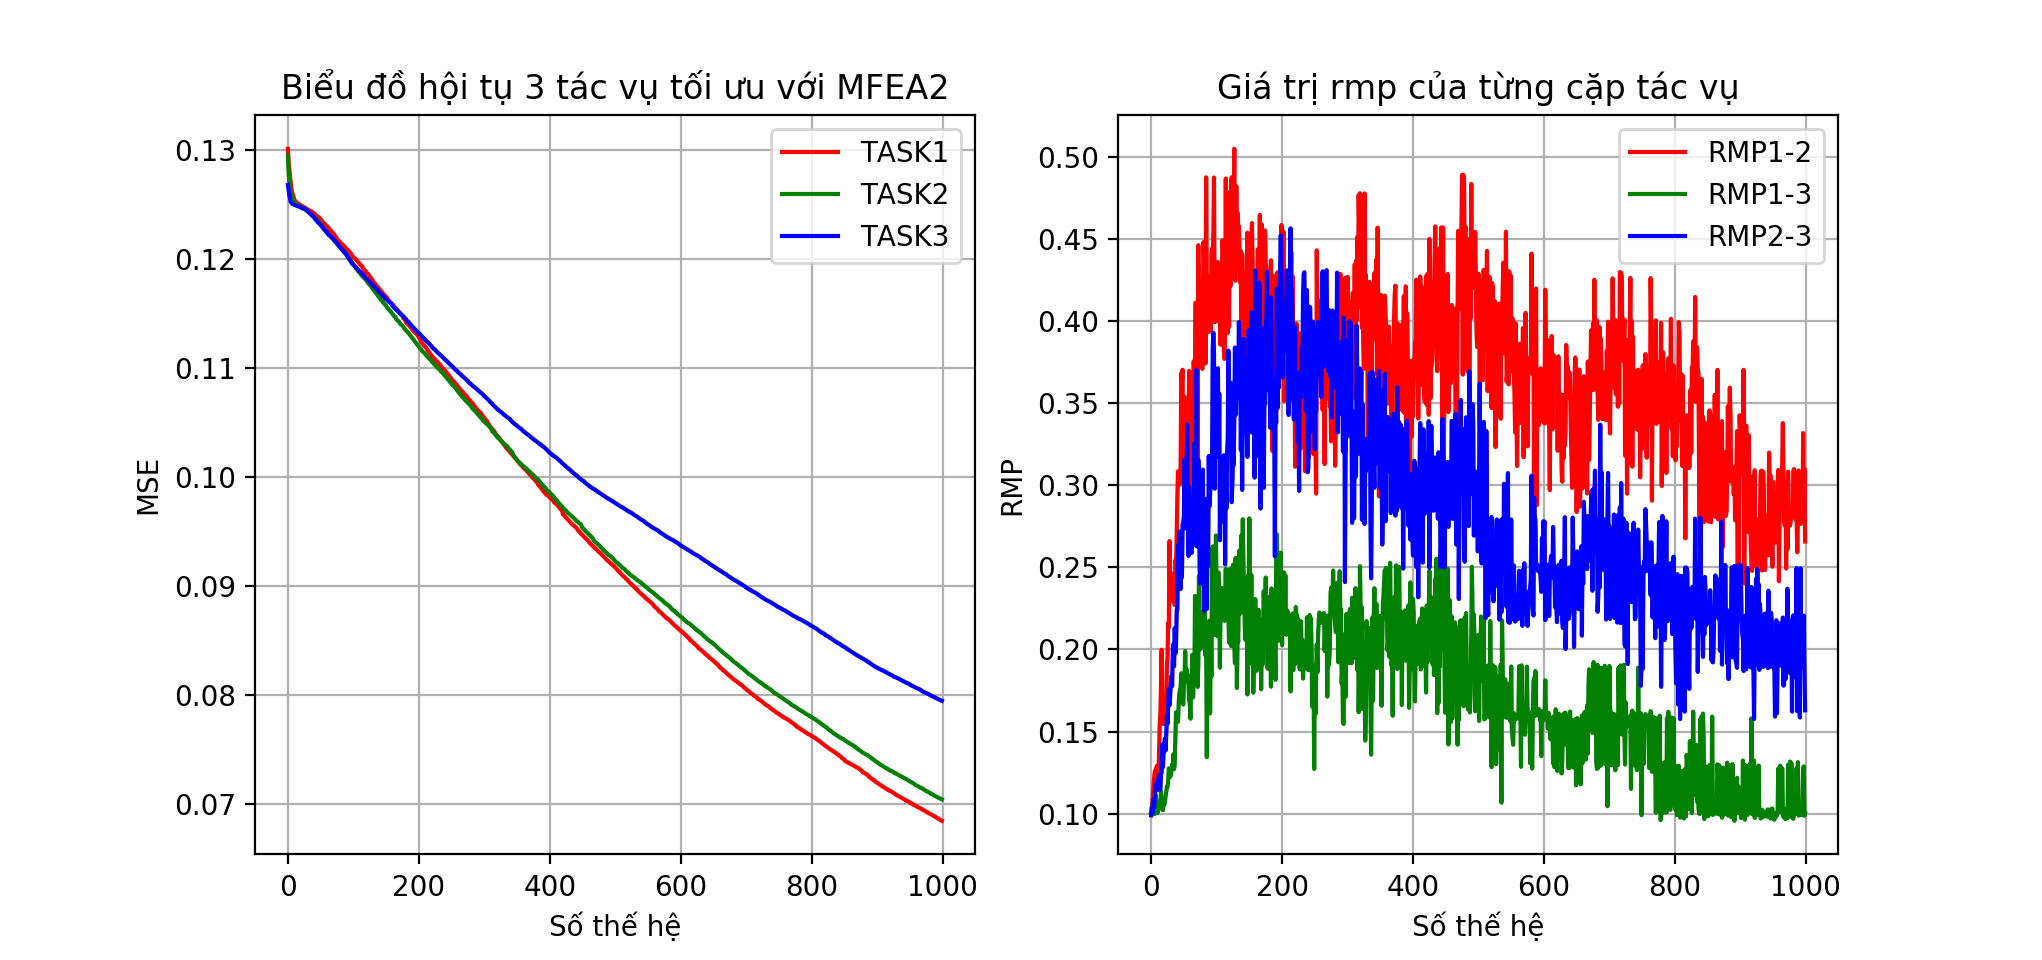
\includegraphics[width=\textwidth,height=\textheight,keepaspectratio]{thesis/images/results/nbit_2layer/9bit1_rmp.png}}
    \caption{Bài 9bit: Biểu đồ hội tụ của từng tác vụ trên các thuật toán và biểu đồ phân tích MFEA-II theo giá trị rmp}
    \label{fig:9bit_2layer}
\end{figure}
\begin{figure}[h!]
    \centering
    \scalebox{.7}{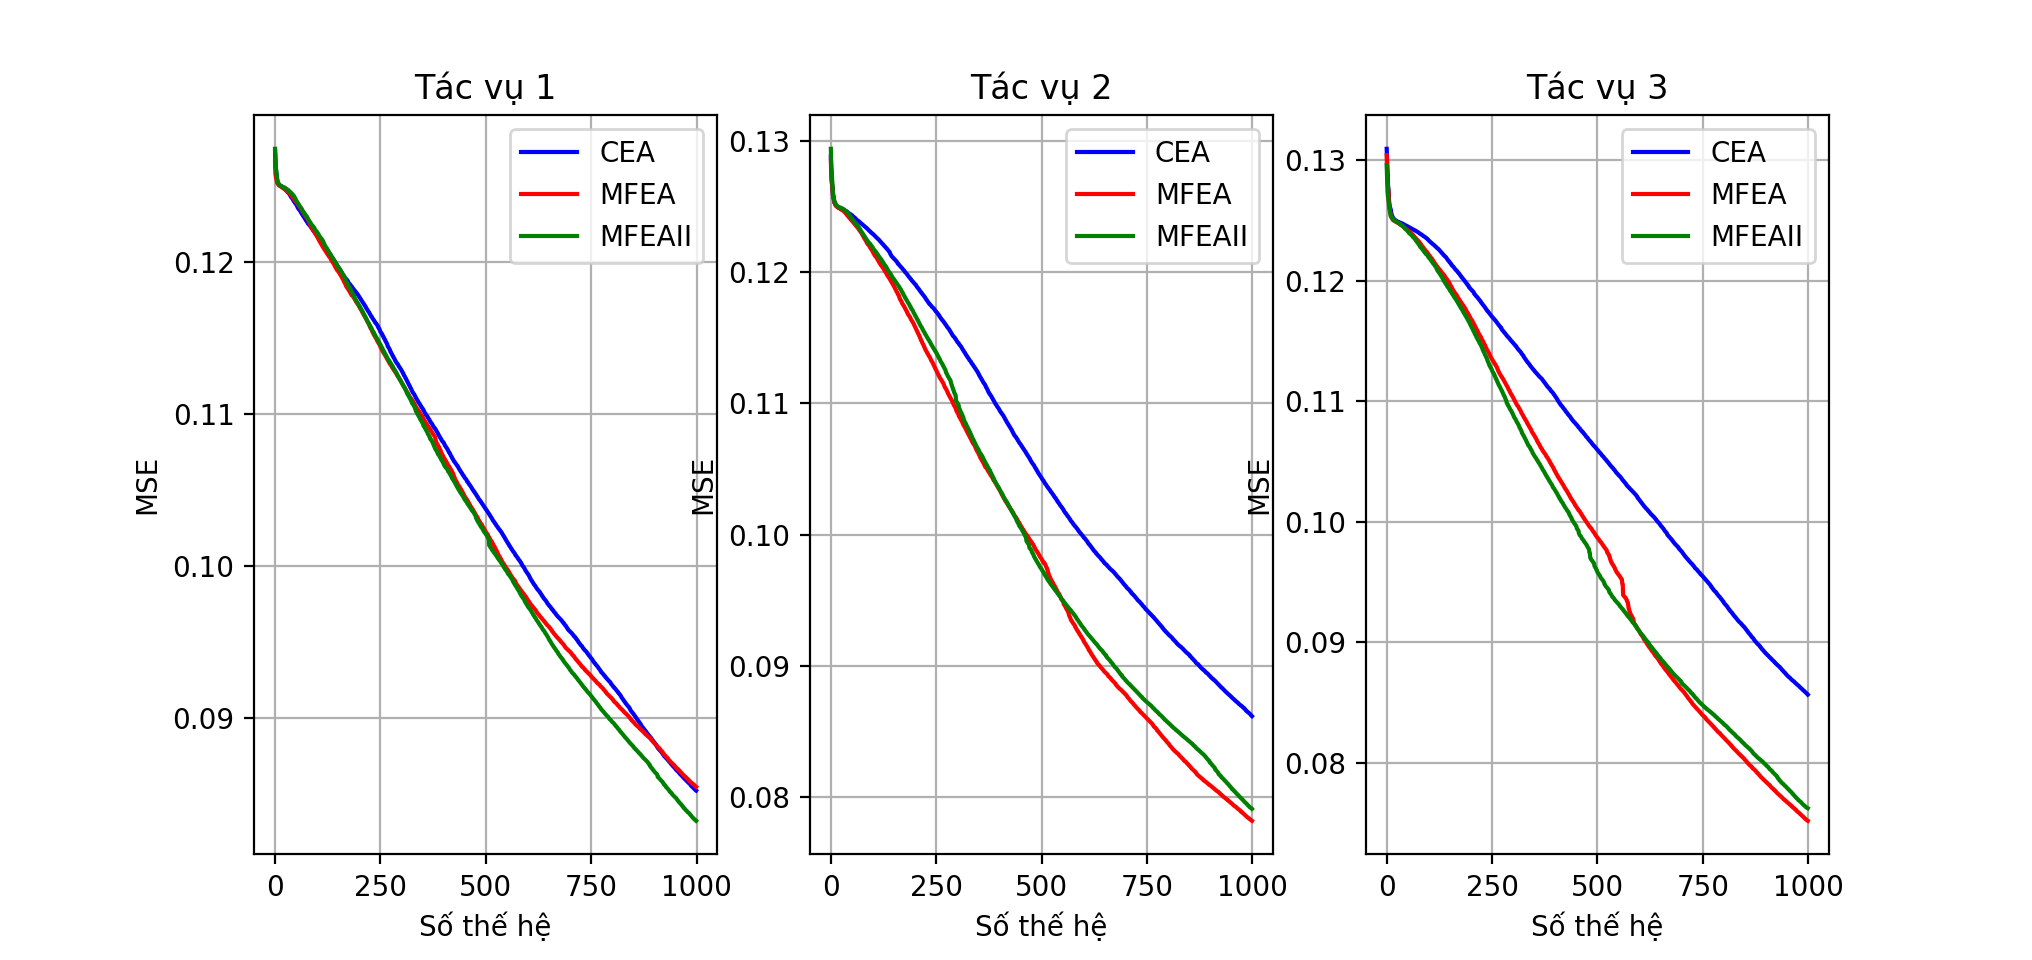
\includegraphics[width=\textwidth,height=\textheight,keepaspectratio]{thesis/images/results/nbit_2layer/10bit1_task.png}}
    \scalebox{.7}{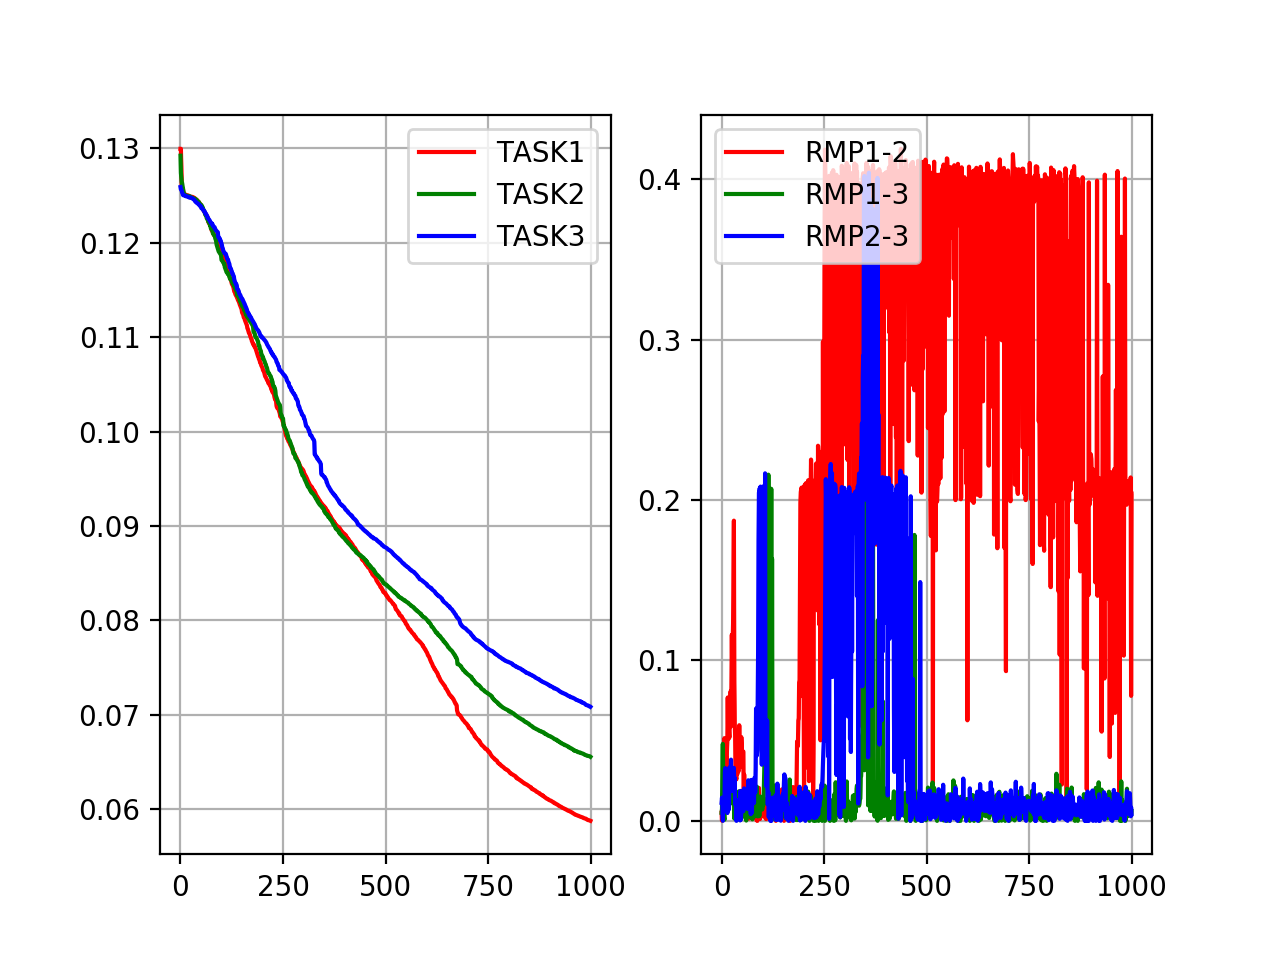
\includegraphics[width=\textwidth,height=\textheight,keepaspectratio]{thesis/images/results/nbit_2layer/10bit1_rmp.png}}
    \caption{Bài 10bit: Biểu đồ hội tụ của từng tác vụ trên các thuật toán và biểu đồ phân tích MFEA-II theo giá trị rmp}
    \label{fig:10bit_2layer}
\end{figure}
\newpage

\subsubsection{Bảng kết quả thực nghiệm - mạng neural khác độ sâu}
\begin{table} [H]
    \begin{center}
    \caption{Kết quả huấn luyện ANN khác độ sâu}
    \begin{tabular}{|c|c|c|c|c|}
    \hline
    \multirow{1}{*}{\textbf{Bài toán}} &
    \multirow{1}{*}{\textbf{Method}} & \multicolumn{1}{c|}{\textbf{Tác vụ 1}} & \multicolumn{1}{c|}{\textbf{Tác vụ 2}} & \multicolumn{1}{c|}{\textbf{Tác vụ 3}} \\ \hline
    \multirow{3}{*} 
    {8-bit} &
    CEA & $0.0789 \pm 0.0172$ & $0.0815 \pm 0.0136$ & $\mathbf{0.0794 \pm 0.0156}$ \\
    & MFEA-I & $0.0778 \pm 0.0153$ & $0.0805 \pm 0.0142$ & $0.0814 \pm 0.0119$  \\
    & MFEA-II & $\mathbf{0.0721} \pm 0.0148$ & $\mathbf{0.0759 \pm 0.015}$ & $0.0822 \pm 0.0143$\\\hline
    \multirow{3}{*} 
    {9-bit} &
    CEA & $0.0843 \pm 0.0154$ & $0.0869 \pm 0.0141$ & $0.086 \pm 0.0128$  \\
    & MFEA-I & $0.0844 \pm 0.0124$ & $\mathbf{0.0795 \pm 0.0144}$ & $\mathbf{0.081 \pm 0.0134}$ \\
    & MFEA-II & $\mathbf{0.0828 \pm 0.0129}$ & $0.0818 \pm 0.0131$ & $0.0864 \pm 0.0147$ \\\hline
    \multirow{3}{*} 
    {10-bit} &
    CEA & $0.089 \pm 0.0131$ & $0.0922 \pm 0.0164$ & $0.0928 \pm 0.0124$  \\
    & MFEA-I  & $0.0879 \pm 0.0091$ & $0.0888 \pm 0.0124$ & $\mathbf{0.0873 \pm 0.0111}$ \\
    & MFEA-II & $\mathbf{0.0867 \pm 0.0079}$ & $\mathbf{0.0862 \pm 0.0103}$ & $0.0905 \pm 0.0104$ \\\hline
    \end{tabular}
    \end{center}
    \label{tab:result:nbit}

\end{table}

\subsubsection{Biểu đồ hội tụ - mạng neural khác độ sâu}

\begin{figure}[h!]
    \centering
    \scalebox{.57}{\includegraphics[width=\textwidth,height=\textheight,keepaspectratio]{thesis/images/results/multilayers/8bit2_task.png}}
    \scalebox{.57}{\includegraphics[width=\textwidth,height=\textheight,keepaspectratio]{thesis/images/results/multilayers/8bit2_rmp.png}}
    \caption{Bài 8bit: Biểu đồ hội tụ của từng tác vụ trên các thuật toán và biểu đồ phân tích MFEA-II theo giá trị rmp}
    \label{fig:8bit_multilayer}
\end{figure}
\begin{figure}[h!]
    \centering
    \scalebox{.6}{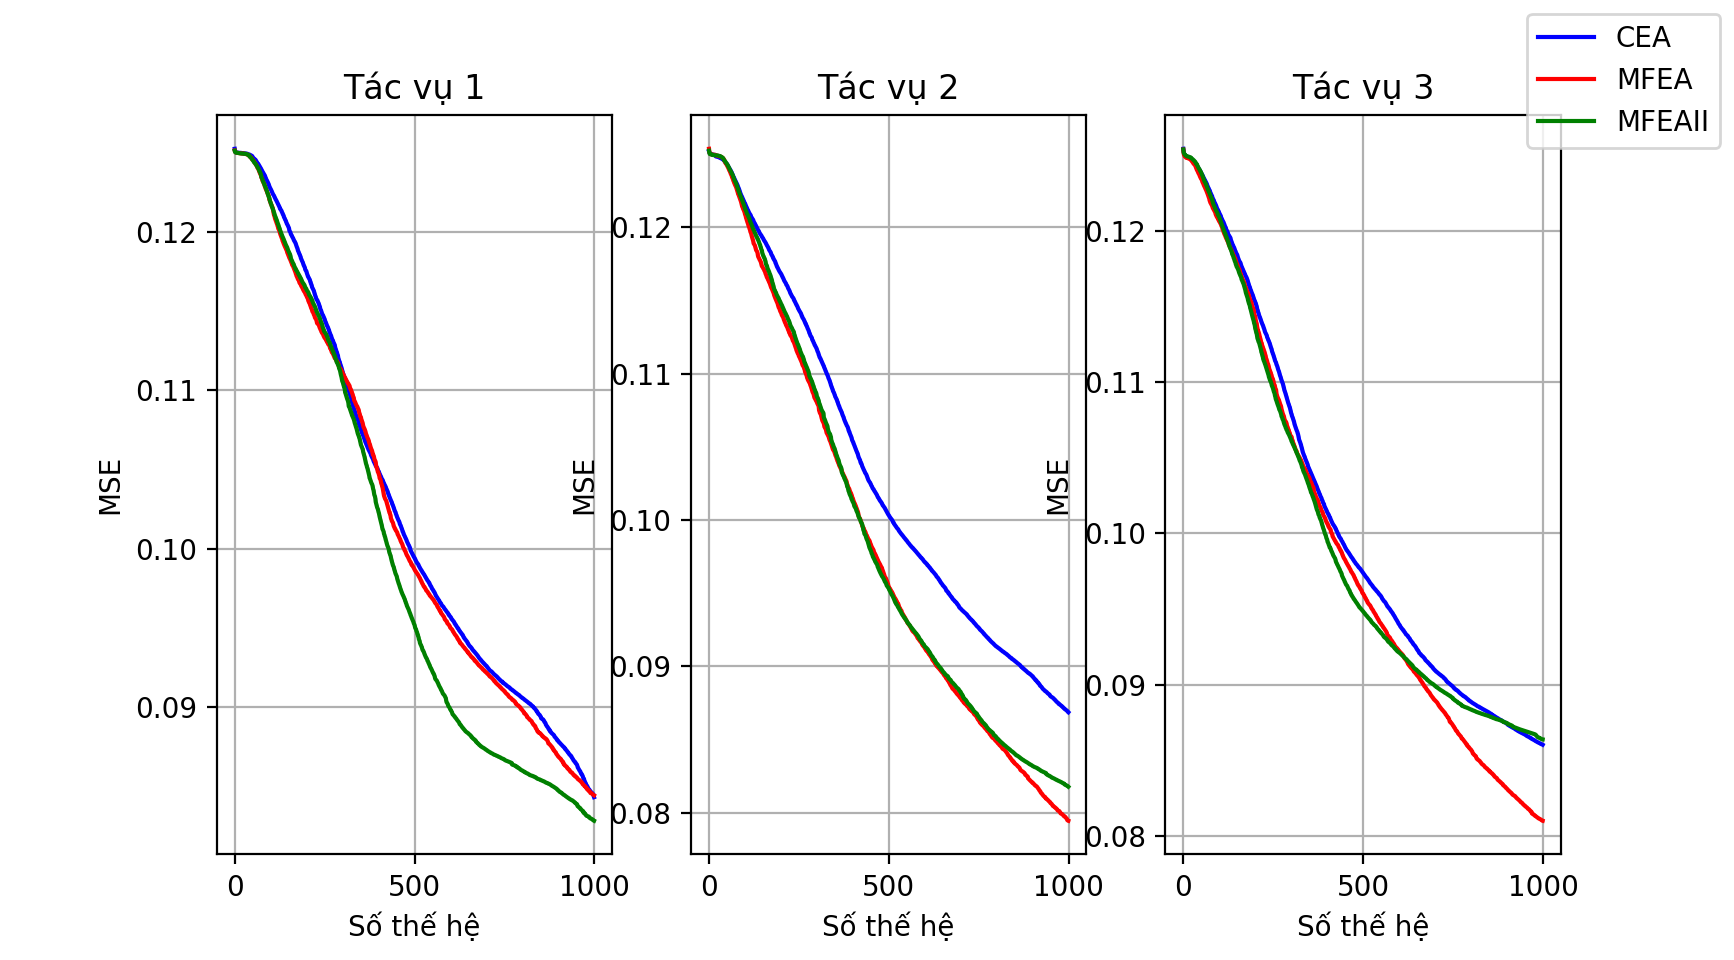
\includegraphics[width=\textwidth,height=\textheight,keepaspectratio]{thesis/images/results/multilayers/9bit2_task.png}}
    \scalebox{.6}{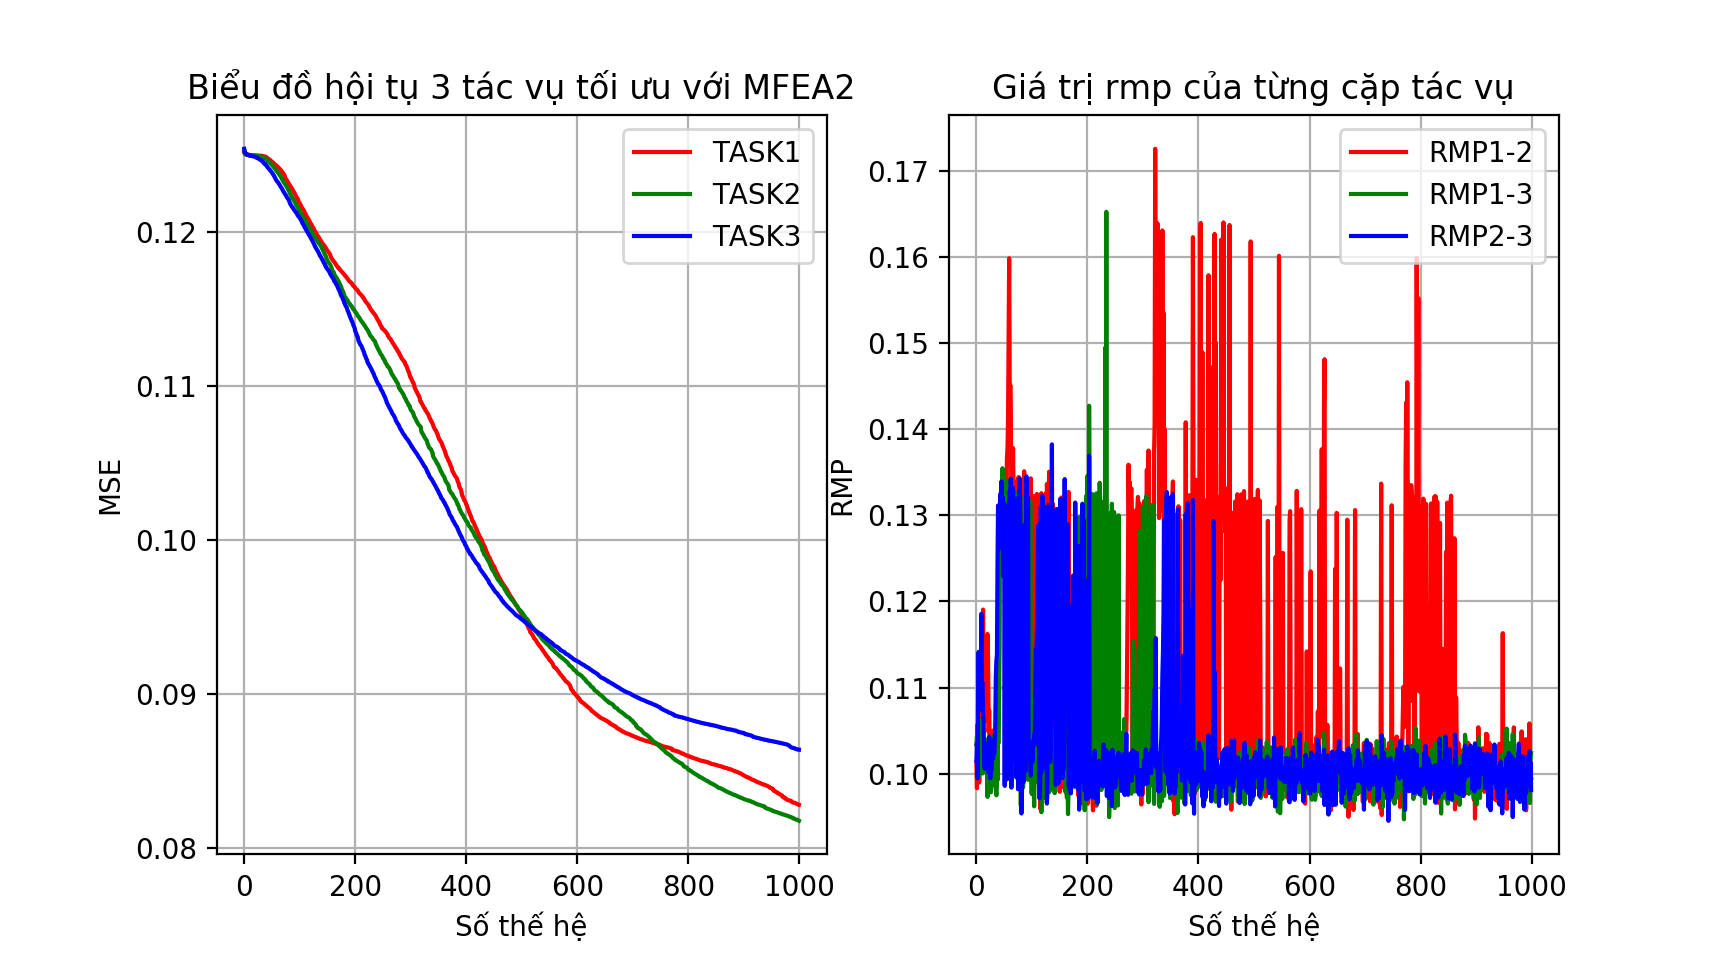
\includegraphics[width=\textwidth,height=\textheight,keepaspectratio]{thesis/images/results/multilayers/9bit2_rmp.png}}
    \caption{Bài 9bit: Biểu đồ hội tụ của từng tác vụ trên các thuật toán và biểu đồ phân tích MFEA-II theo giá trị rmp}
    \label{fig:8bit_multilayer}
\end{figure}
\begin{figure}[h!]
    \centering
    \scalebox{.5}{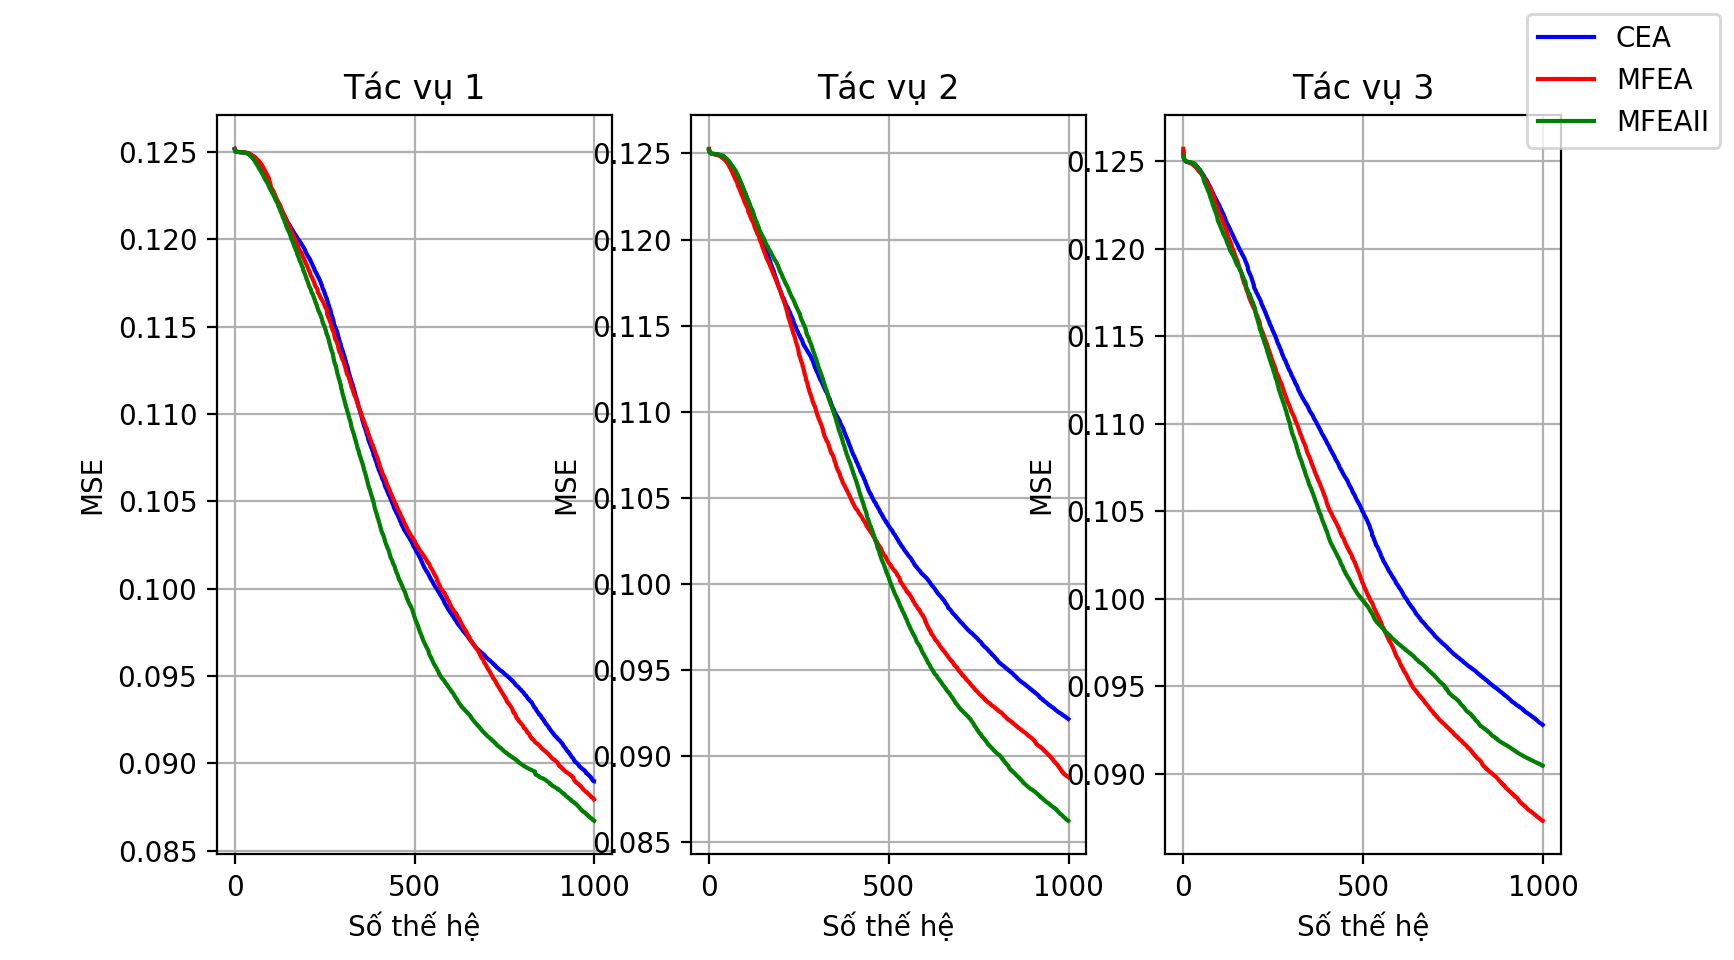
\includegraphics[width=\textwidth,height=\textheight,keepaspectratio]{thesis/images/results/multilayers/10bit2_task.png}}
    \scalebox{.5}{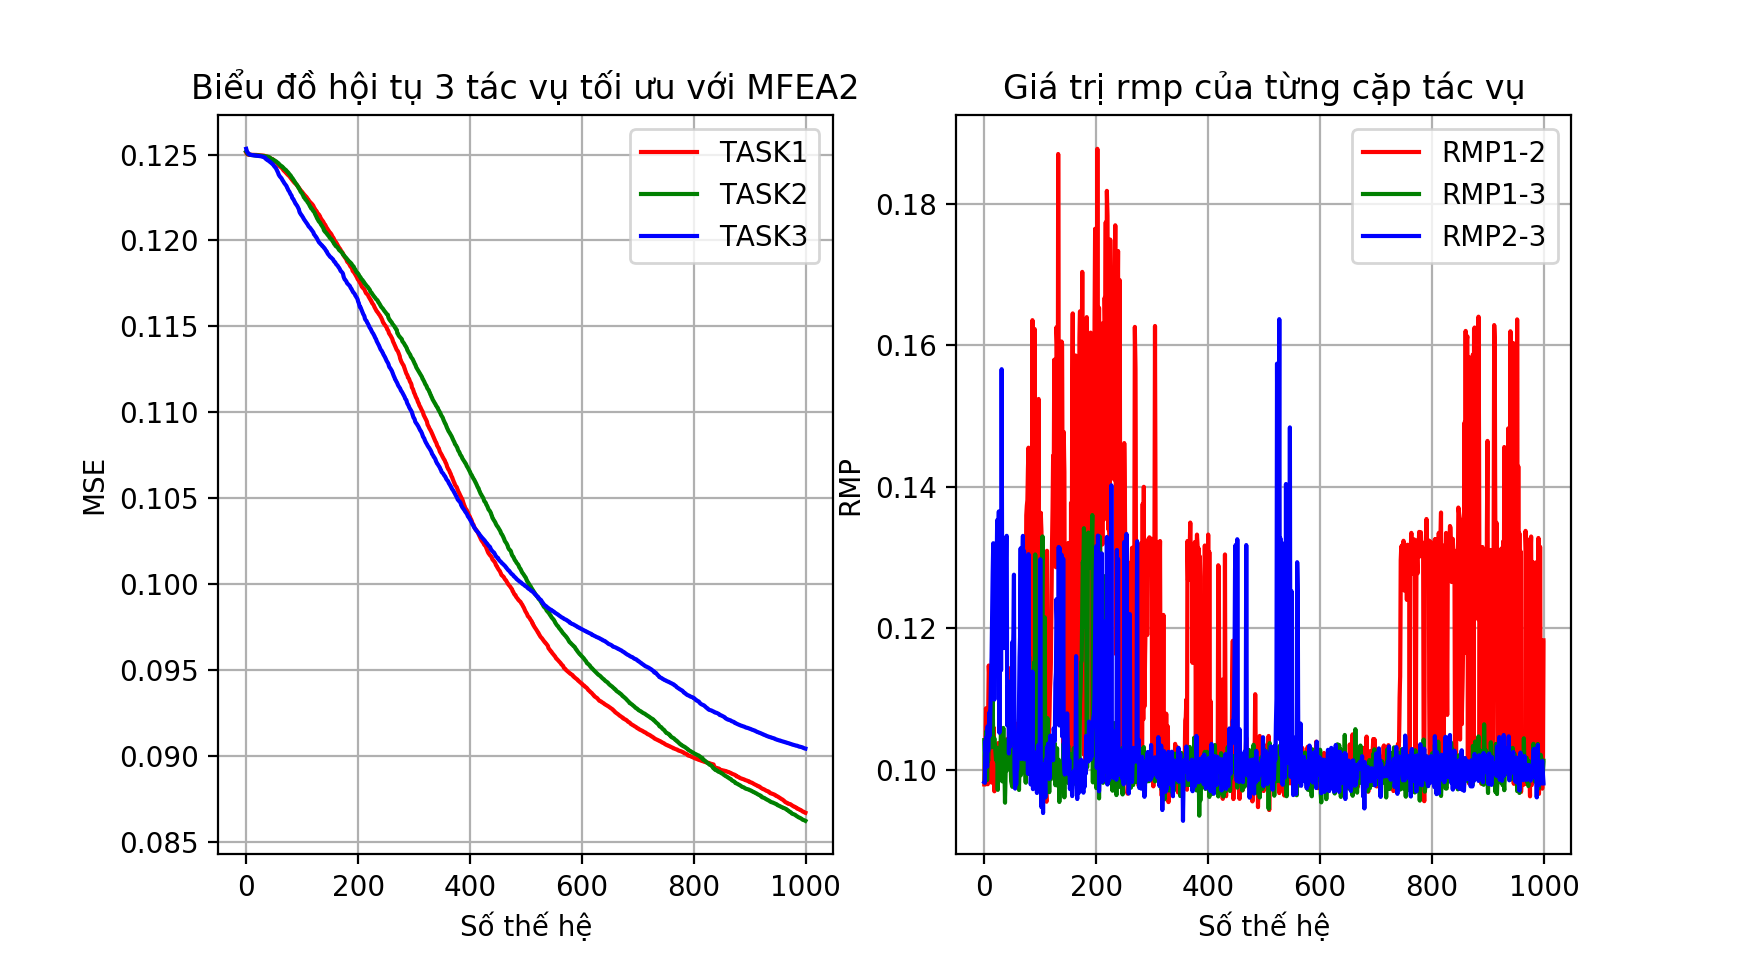
\includegraphics[width=\textwidth,height=\textheight,keepaspectratio]{thesis/images/results/multilayers/10bit2_rmp.png}}
    \caption{Bài 10bit: Biểu đồ hội tụ của từng tác vụ trên các thuật toán và biểu đồ phân tích MFEA-II theo giá trị rmp}
    \label{fig:8bit_multilayer}
\end{figure}

\subsubsection{Bảng kết quả thực nghiệm - bộ dữ liệu UCI với mạng neural cùng độ sâu}
\begin{table}[h!]
    \caption{Kết quả huấn luyện nhiều ANN trên bộ dữ liệu UCI cùng độ sâu}

    \begin{tabular}{|c|c|c|c|c|}
    \hline
    \multirow{1}{*}{\textbf{Instance}} & \multicolumn{1}{c|} {\textbf{Method}} & \multicolumn{1}{c|}{\textbf{Subtask1}} & \multicolumn{1}{c|}{\textbf{Subtask 2}} & \multicolumn{1}{c|}{\textbf{Subtask 3}} \\ \hline
    \multirow{3}{*} 
    {breastCancer} & CEA & $0.0097 \pm 0.0012$ & $0.0092 \pm 0.0007$ & $0.0093 \pm 0.0009$ \\
     & MFEA-I & $0.0097 \pm 0.0006$ & $0.0093 \pm 0.0005$ & $0.0091 \pm 0.0005$ \\ 
    & MFEA II & $\mathbf{0.0094 \pm 0.0008}$ & $\mathbf{0.0089 \pm 0.0006}$ & $\mathbf{0.0087 \pm 0.0004}$ \\ \hline
    \multirow{3}{*} {creditScreening} & CEA & $0.0509 \pm 0.0033$ & $0.0514 \pm 0.0033$ & $0.0508 \pm 0.004$ \\
   & MFEA-I & $0.0504 \pm 0.0024$ & $0.0503 \pm 0.0025$ & $0.0513 \pm 0.0022$ \\ 
   & MFEA-II & $\mathbf{0.0492 \pm 0.0023}$ & $\mathbf{0.0489 \pm 0.002}$ & $\mathbf{0.0491 \pm 0.002}$ \\ \hline
    \multirow{3}{*} {ionosphere} & CEA & $0.0384 \pm 0.0072$ & $0.0389 \pm 0.0129$ & $0.035 \pm 0.0047$ \\
    &MFEA-I & $0.0367 \pm 0.0068$ & $0.0347 \pm 0.0075$ & $0.0351 \pm 0.0088$ \\
    &MFEA-II & $\mathbf{0.0343 \pm 0.0079}$ & $\mathbf{0.0322 \pm 0.0071}$ & $\mathbf{0.032 \pm 0.007}$ \\\hline
    \multirow{3}{*} {ticTacToe} & CEA & $0.089 \pm 0.0047$ & $0.0838 \pm 0.0054$ & $0.0869 \pm 0.0049$ \\
    &MFEA-I & $0.0845 \pm 0.0049$ & $0.0818 \pm 0.0047$ & $0.0824 \pm 0.0047$ \\
    &MFEA-II & $\mathbf{0.082 \pm 0.0048}$ & $\mathbf{0.0815 \pm 0.0046}$ & $\mathbf{0.0812 \pm 0.0043}$  \\\hline
    
    \end{tabular}

    \label{tab:result:nbit}
\end{table}
\subsubsection{Biểu đồ hội tụ - bộ dữ liệu UCI với mạng neural cùng độ sâu}

\begin{figure}[h!]
    \centering
    \scalebox{.7}{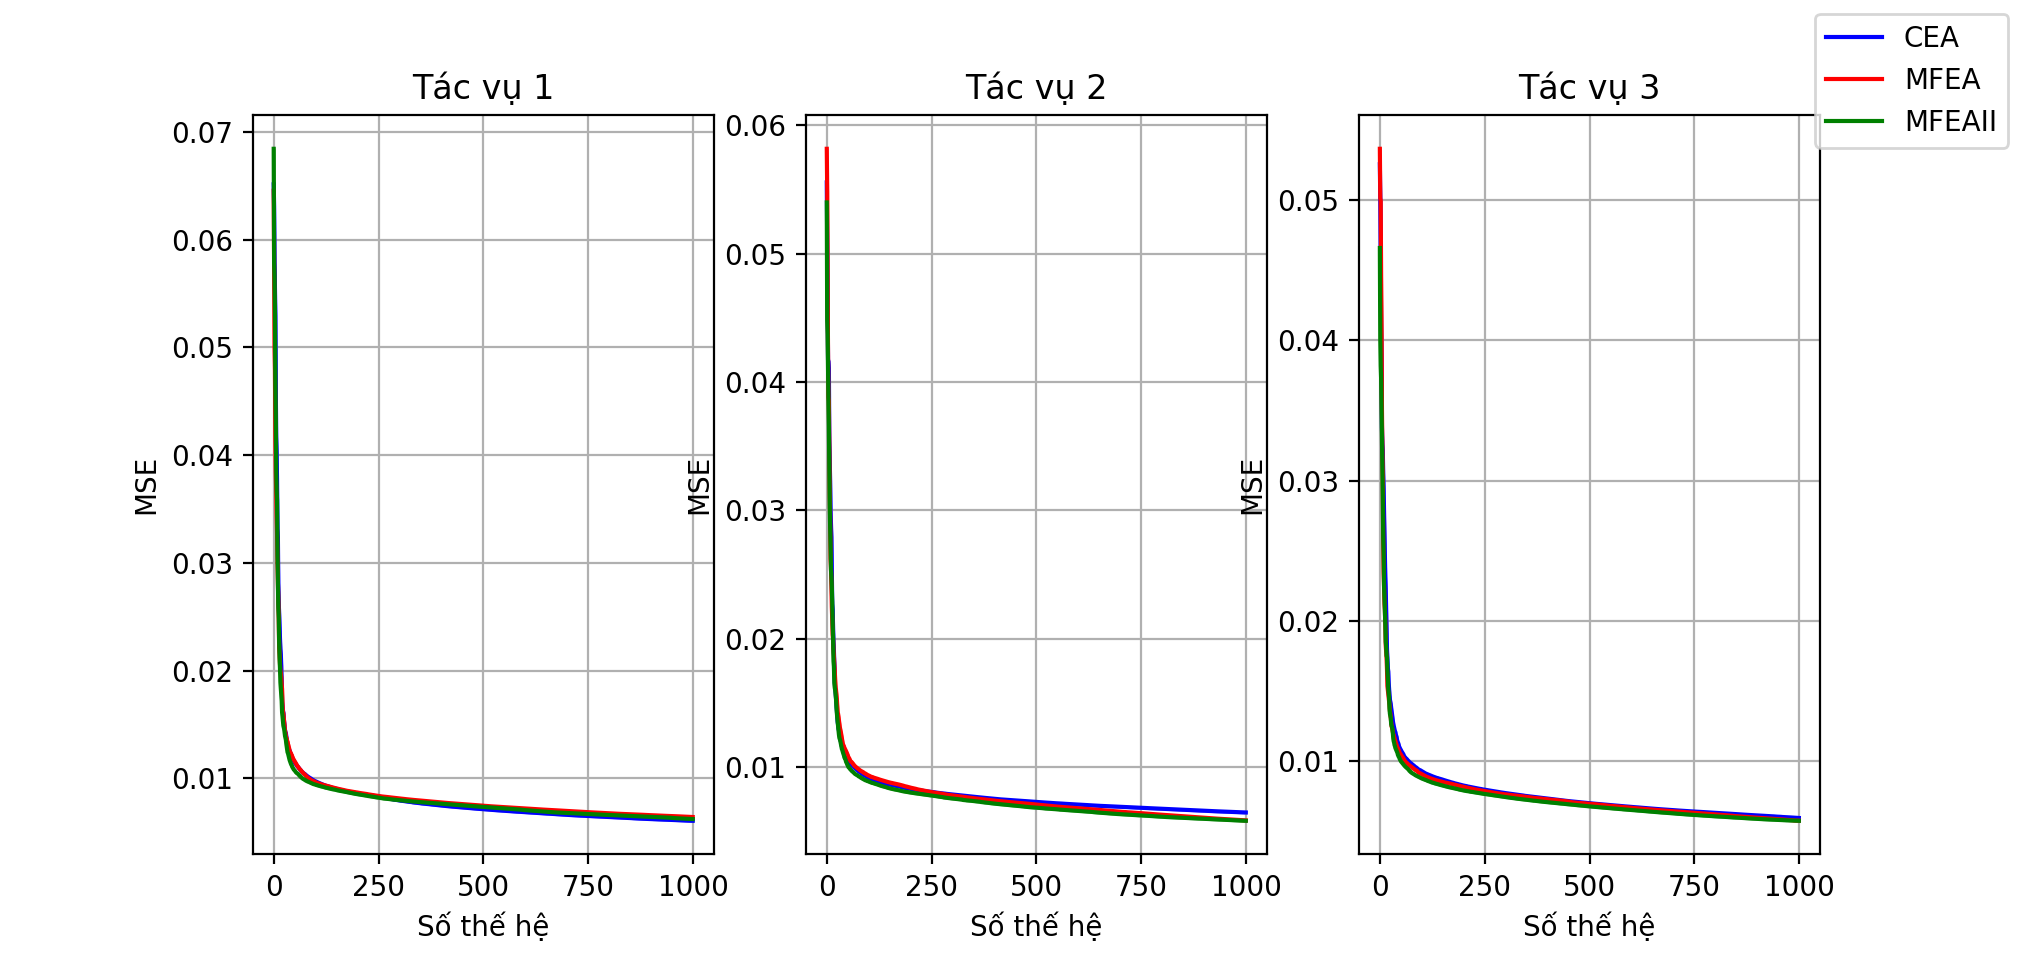
\includegraphics[width=\textwidth,height=\textheight,keepaspectratio]{thesis/images/results/uci/br1_task.png}}
    \scalebox{.7}{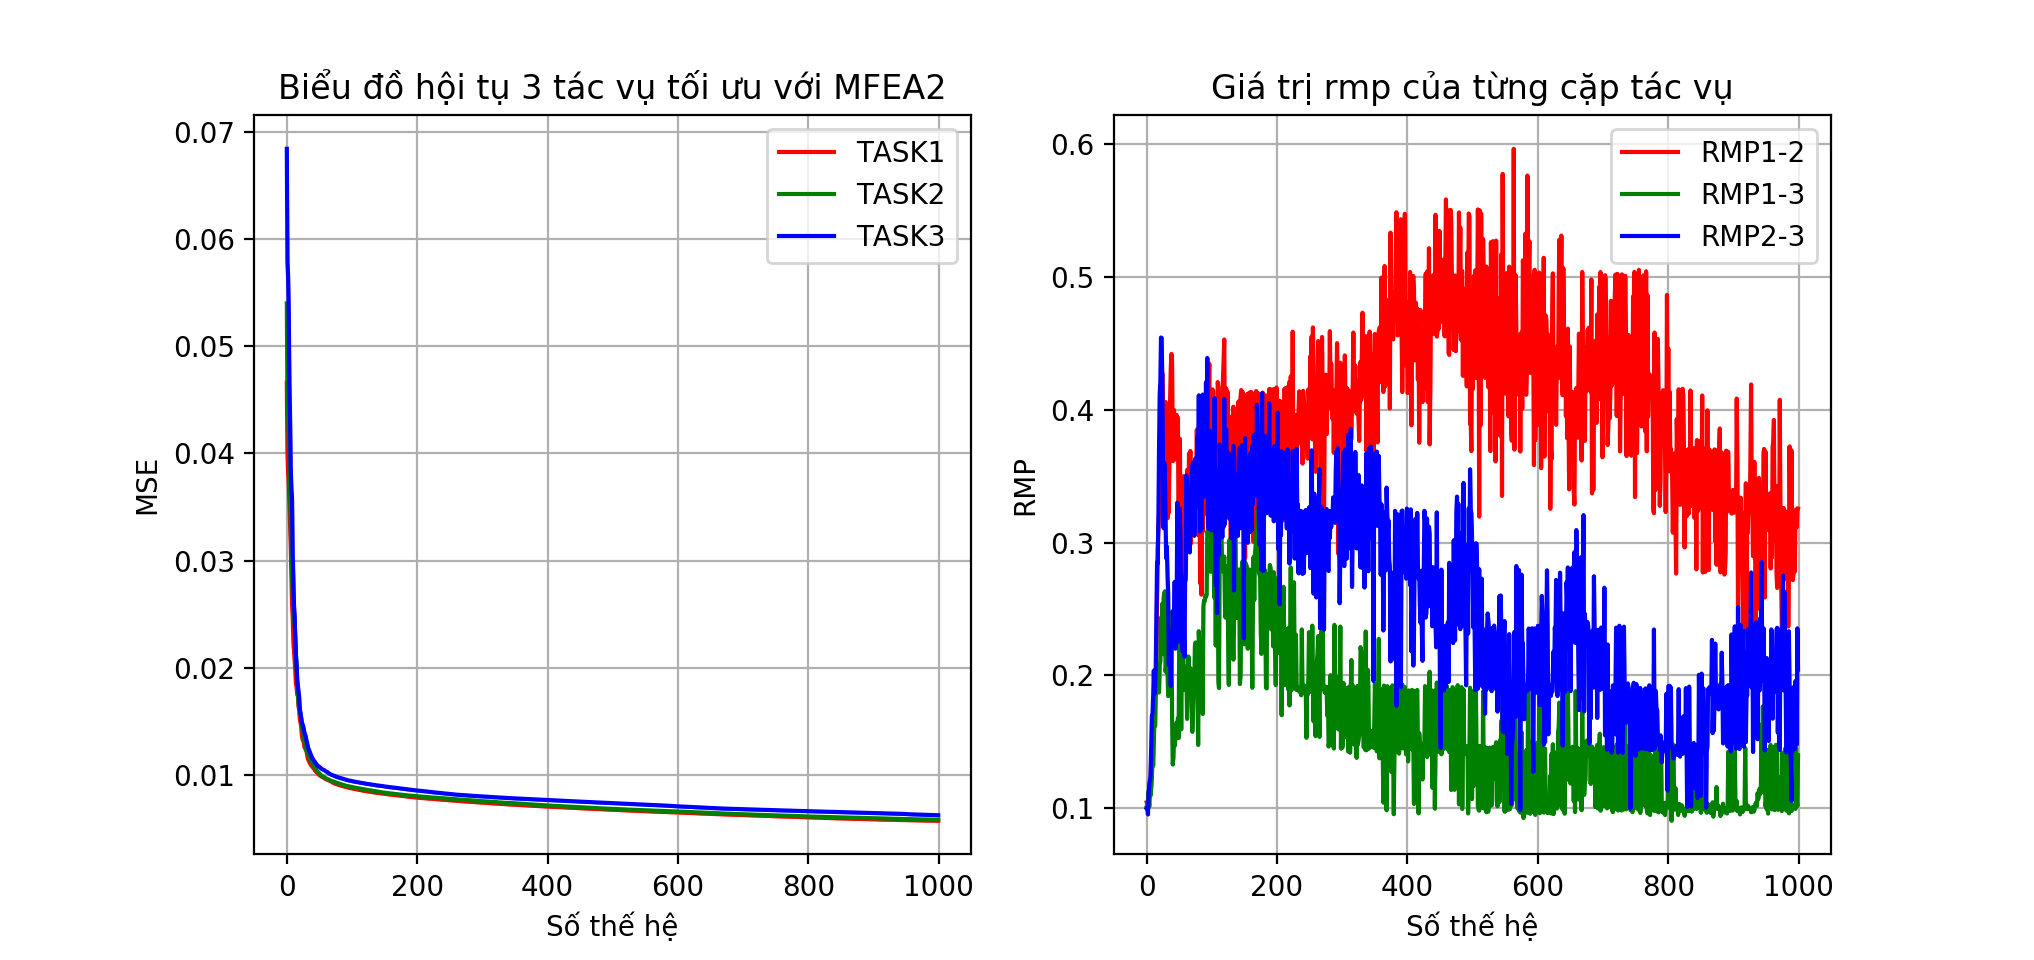
\includegraphics[width=\textwidth,height=\textheight,keepaspectratio]{thesis/images/results/uci/br1_rmp.png}}
    \caption{Biểu đồ hội tụ của các tác vụ bài BreastCancer cùng độ sâu}
    \label{fig:br_mtl}
\end{figure}

\begin{figure}[h!]
    \centering
    \scalebox{.7}{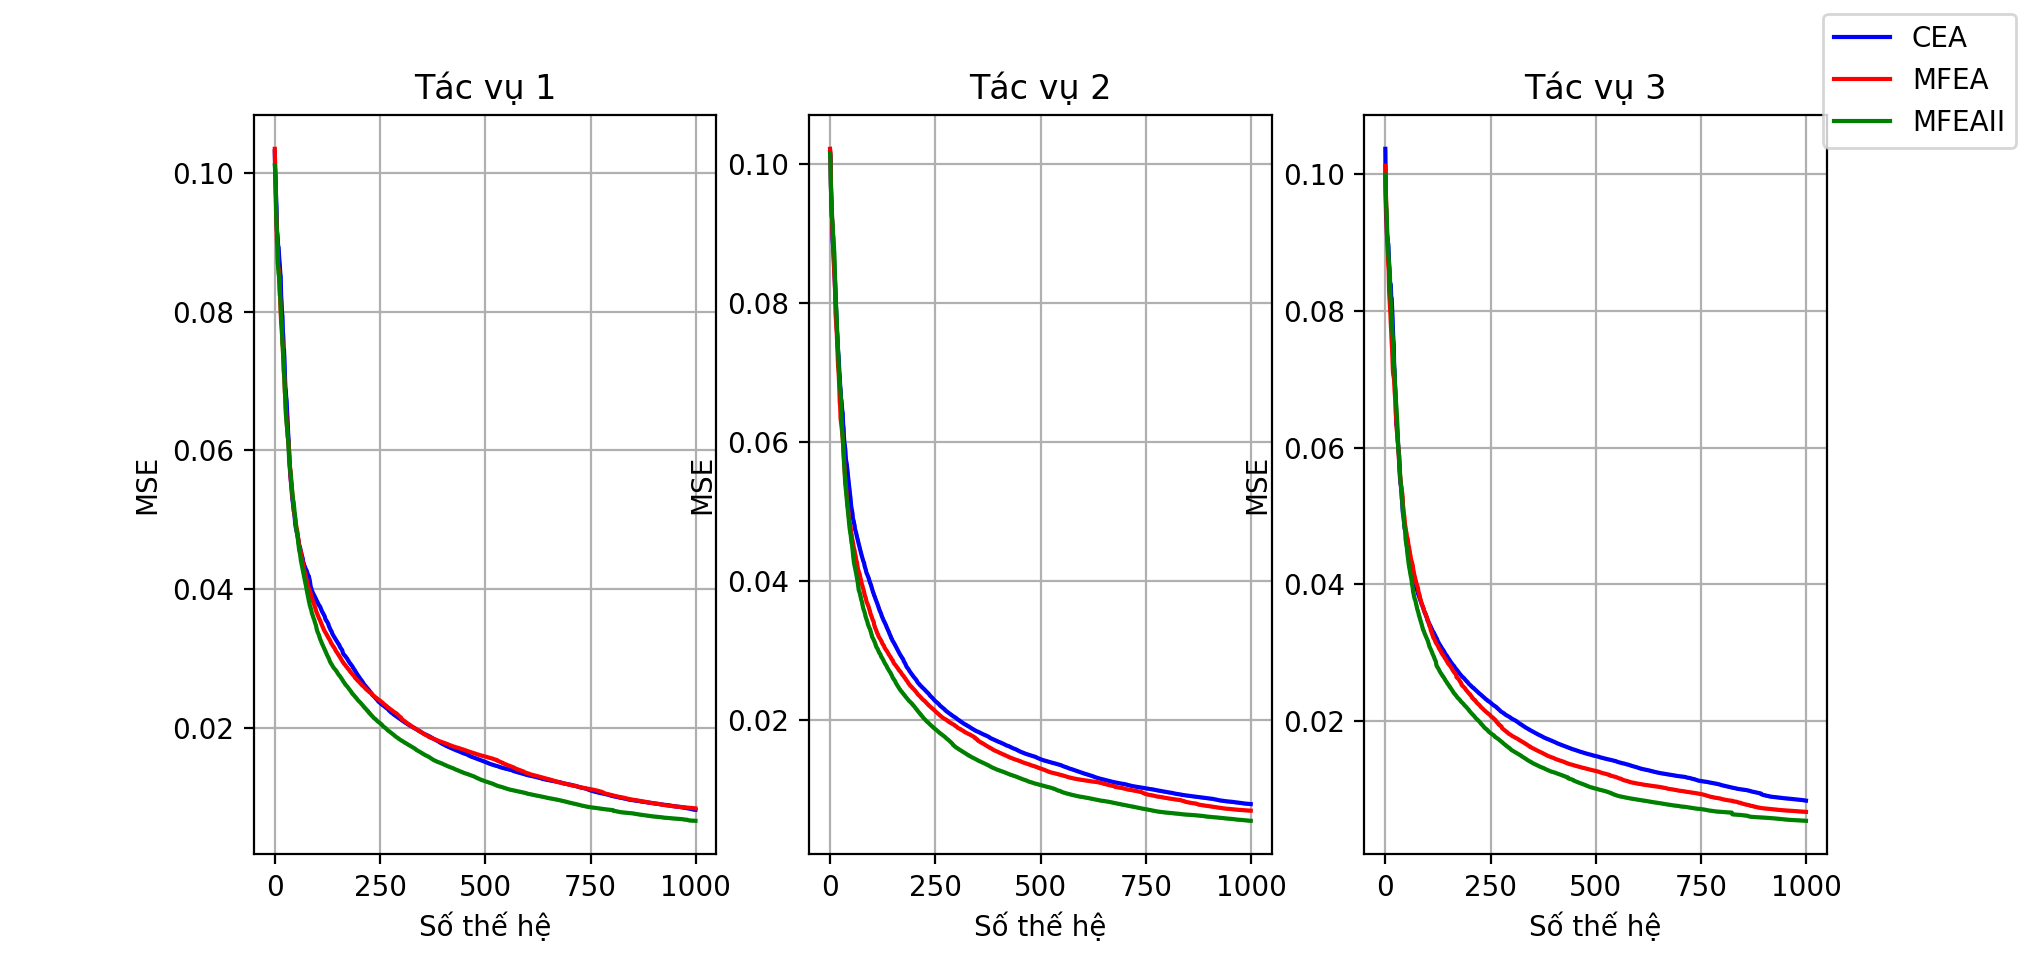
\includegraphics[width=\textwidth,height=\textheight,keepaspectratio]{thesis/images/results/uci/is1_task.png}}
    \scalebox{.7}{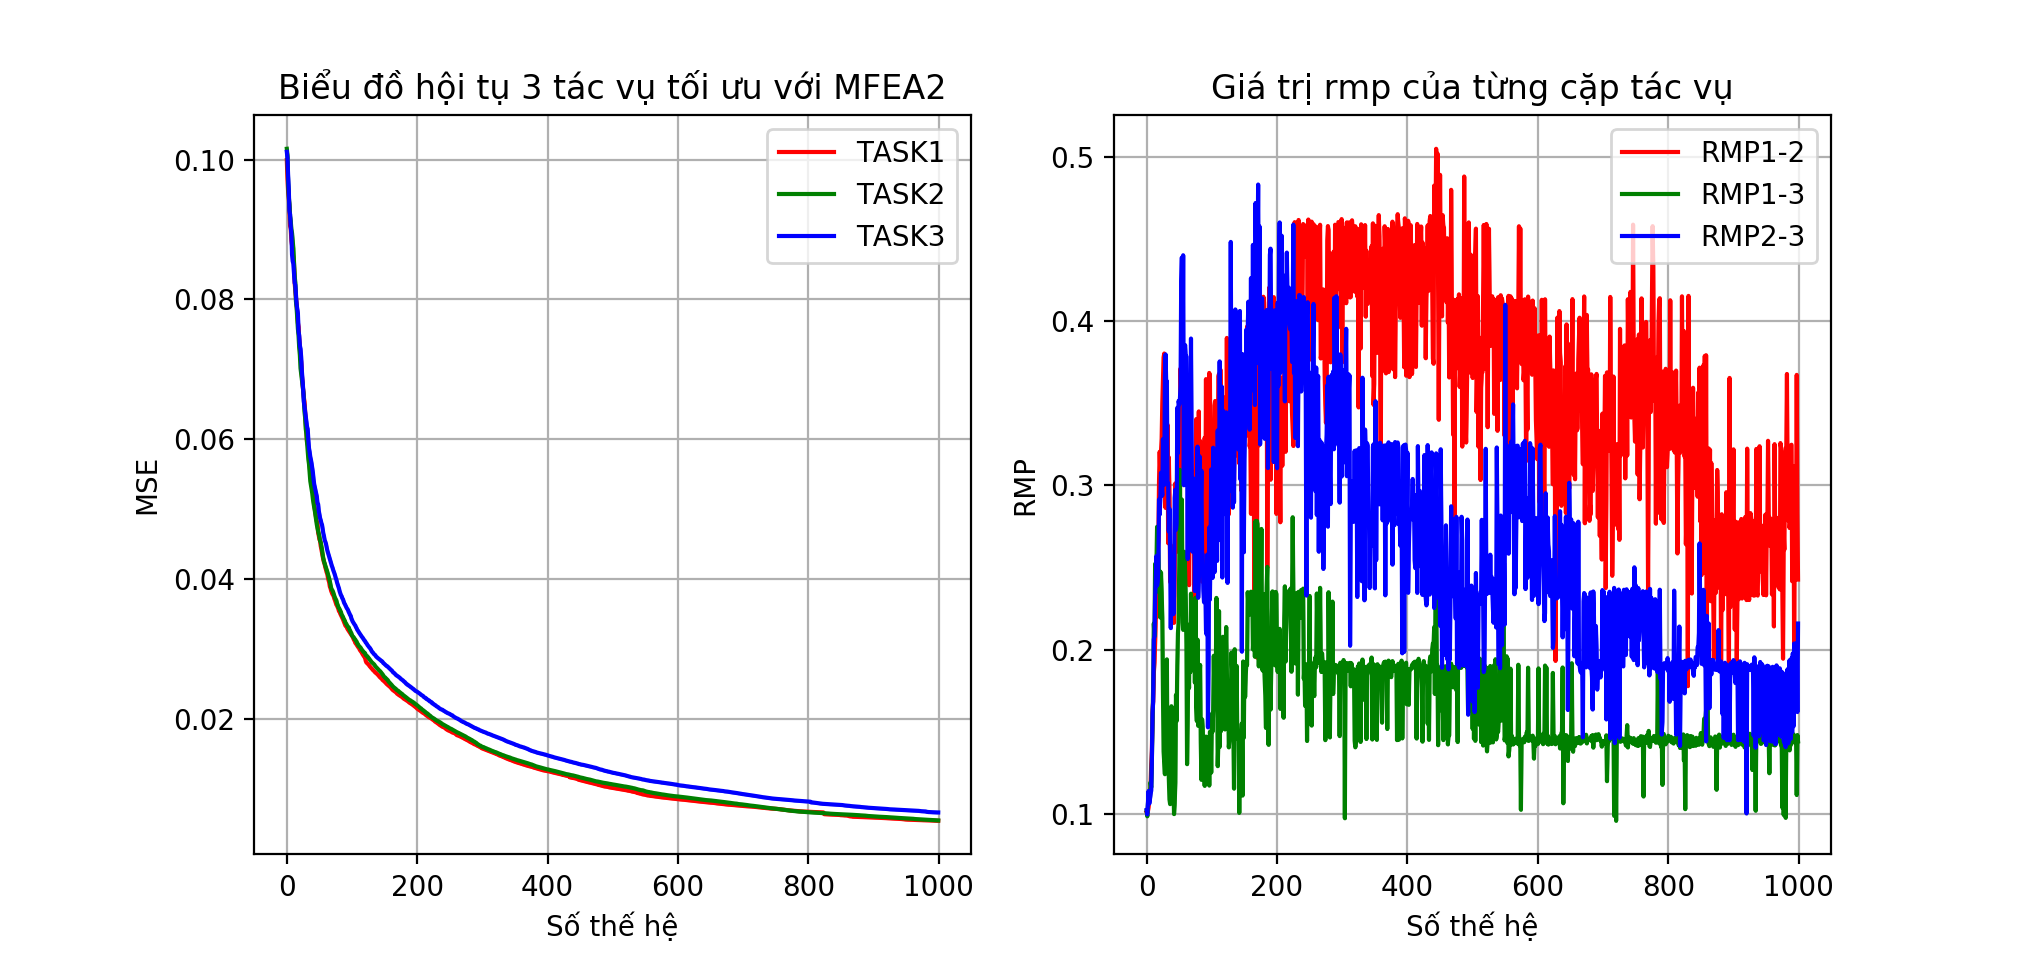
\includegraphics[width=\textwidth,height=\textheight,keepaspectratio]{thesis/images/results/uci/is1_rmp.png}}
    \caption{Biểu đồ hội tụ của các tác vụ bài Ionosphere cùng độ sâu}
    \label{fig:br_mtl}
\end{figure}
\newpage
\subsubsection{Bảng kết quả thực nghiệm - bộ dữ liệu UCI với mạng neural khác độ sâu}
% \begin{table}[h!]
%     \caption{Huấn luyện nhiều ANN trên bộ dữ liệu UCI khác độ sâu}
%     \begin{tabular}{|c|c|c|c|c|}
%     \hline
%     \multirow{1}{*}{\textbf{Instance}} & \multicolumn{1}{c|} {\textbf{Method}} & \multicolumn{1}{c|}{\textbf{Subtask1}} & \multicolumn{1}{c|}{\textbf{Subtask 2}} & \multicolumn{1}{c|}{\textbf{Subtask 3}} \\ \hline
%     \multirow{3}{*} 
%     {breastCancer} & CEA & $0.0119 \pm 0.0029$ & $0.0107 \pm 0.002$ & $\mathbf{0.0093 \pm 0.0005}$ \\
%      & MFEA-I & $\mathbf{0.011 \pm 0.0015}$ & $0.0102 \pm 0.0012$ & $0.0094 \pm 0.0005$  \\ 
%     & MFEA II & $\mathbf{0.011 \pm 0.0015}$ & $\mathbf{0.01 \pm 0.0011}$ & $0.0096 \pm 0.0011$ \\ \hline
    
%     \multirow{3}{*} {creditScreening} & CEA & $0.054 \pm 0.0071$ & $0.0503 \pm 0.0027$ & $0.0485 \pm 0.0017$ \\
%   & MFEA-I & $\mathbf{0.0508 \pm 0.0023}$ & $0.0497 \pm 0.0019$ & $0.0496 \pm 0.0021$ \\ 
%   & MFEA-II & $0.0515 \pm 0.0033$ & $\mathbf{0.0494 \pm 0.0023}$ & $\mathbf{0.0485 \pm 0.0018}$ \\ \hline
   
%     \multirow{3}{*} {ionosphere} & CEA & $0.0516 \pm 0.0124$ & $0.0449 \pm 0.0114$ & $0.0366 \pm 0.0094$ \\
%     &MFEA-I & $0.049 \pm 0.0131$ & $0.0413 \pm 0.0112$ & $\mathbf{0.0365 \pm 0.007}$ \\
%     &MFEA-II & $\mathbf{0.0473 \pm 0.0083}$ & $\mathbf{0.0387 \pm 0.0109}$ & $0.0367 \pm 0.008$  \\\hline
    
%     \multirow{3}{*} {ticTacToe} & CEA & $0.0899 \pm 0.0067$ & $0.0879 \pm 0.0079$ & $0.0852 \pm 0.0045$  \\
%     &MFEA-I & $\mathbf{0.088 \pm 0.008}$ & $0.0886 \pm 0.0064$ & $0.0843 \pm 0.0092$  \\
%     &MFEA-II & $\mathbf{0.088 \pm 0.0073}$ & $\mathbf{0.0832 \pm 0.0067}$ & $0\mathbf{.0817 \pm 0.0046}$  \\\hline
    
%     \end{tabular}

%     \label{tab:result:nbit}
% \end{table}
\begin{table}[h!]
    \caption{Kết quả huấn luyện nhiều ANN trên bộ dữ liệu UCI khác độ sâu}
    \begin{tabular}{|c|c|c|c|c|}
    \hline
    \multirow{1}{*}{\textbf{Instance}} & \multicolumn{1}{c|} {\textbf{Method}} & \multicolumn{1}{c|}{\textbf{Subtask1}} & \multicolumn{1}{c|}{\textbf{Subtask 2}} & \multicolumn{1}{c|}{\textbf{Subtask 3}} \\ \hline
    \multirow{3}{*} 
    {breastCancer} & CEA & $0.0082 \pm 0.0006$ & $0.0083 \pm 0.0006$ & $0.008 \pm 0.0004$ \\
     & MFEA-I & $0.0084 \pm 0.0007$ & $0.0081 \pm 0.0006$ & $0.008 \pm 0.0004$  \\ 
    & MFEA II & $\mathbf{0.0082 \pm 0.0006}$ & $\mathbf{0.008 \pm 0.0004}$ & $\mathbf{0.008 \pm 0.0004}$ \\ \hline
    
    \multirow{3}{*} {creditScreening} & CEA & $0.0442 \pm 0.0016$ & $0.0436 \pm 0.0011$ & $0.0435 \pm 0.0011$ \\
   & MFEA-I & $0.0446 \pm 0.0017$ & $\mathbf{0.0435 \pm 0.0012}$ & $0.0438 \pm 0.0013$ \\ 
   & MFEA-II & $\mathbf{0.0442 \pm 0.0016}$ & $0.0437 \pm 0.0014$ & $\mathbf{0.0433 \pm 0.0012}$ \\ \hline
   
    \multirow{3}{*} {ionosphere} & CEA & $\mathbf{0.0223 \pm 0.0064}$ & $\mathbf{0.0189 \pm 0.005}$ & $\mathbf{0.018 \pm 0.0063}$ \\
    &MFEA-I & $0.0257 \pm 0.01$ & $0.0213 \pm 0.0082$ & $0.0201 \pm 0.0076$ \\
    &MFEA-II & $0.0243 \pm 0.0055$ & $0.0199 \pm 0.0055$ & $0.0203 \pm 0.0062$  \\\hline
    
    \multirow{3}{*} {ticTacToe} & CEA & $0.0747 \pm 0.0077$ & $0.0728 \pm 0.0093$ & $0.0731 \pm 0.0061$   \\
    &MFEA-I & $0.0736 \pm 0.0103$ & $0.0724 \pm 0.008$ & $0.0704 \pm 0.0067$   \\
    &MFEA-II & $\mathbf{0.0709 \pm 0.0096}$ & $\mathbf{0.0667 \pm 0.0066}$ & $\mathbf{0.0684 \pm 0.0067}$  \\\hline
    
    \end{tabular}

    \label{tab:result:nbit}
\end{table}

\newpage
\subsubsection{Biểu đồ hội tụ - bộ dữ liệu UCI với mạng neural cùng độ sâu}

\begin{figure}[h!]
    \centering
    \scalebox{.7}{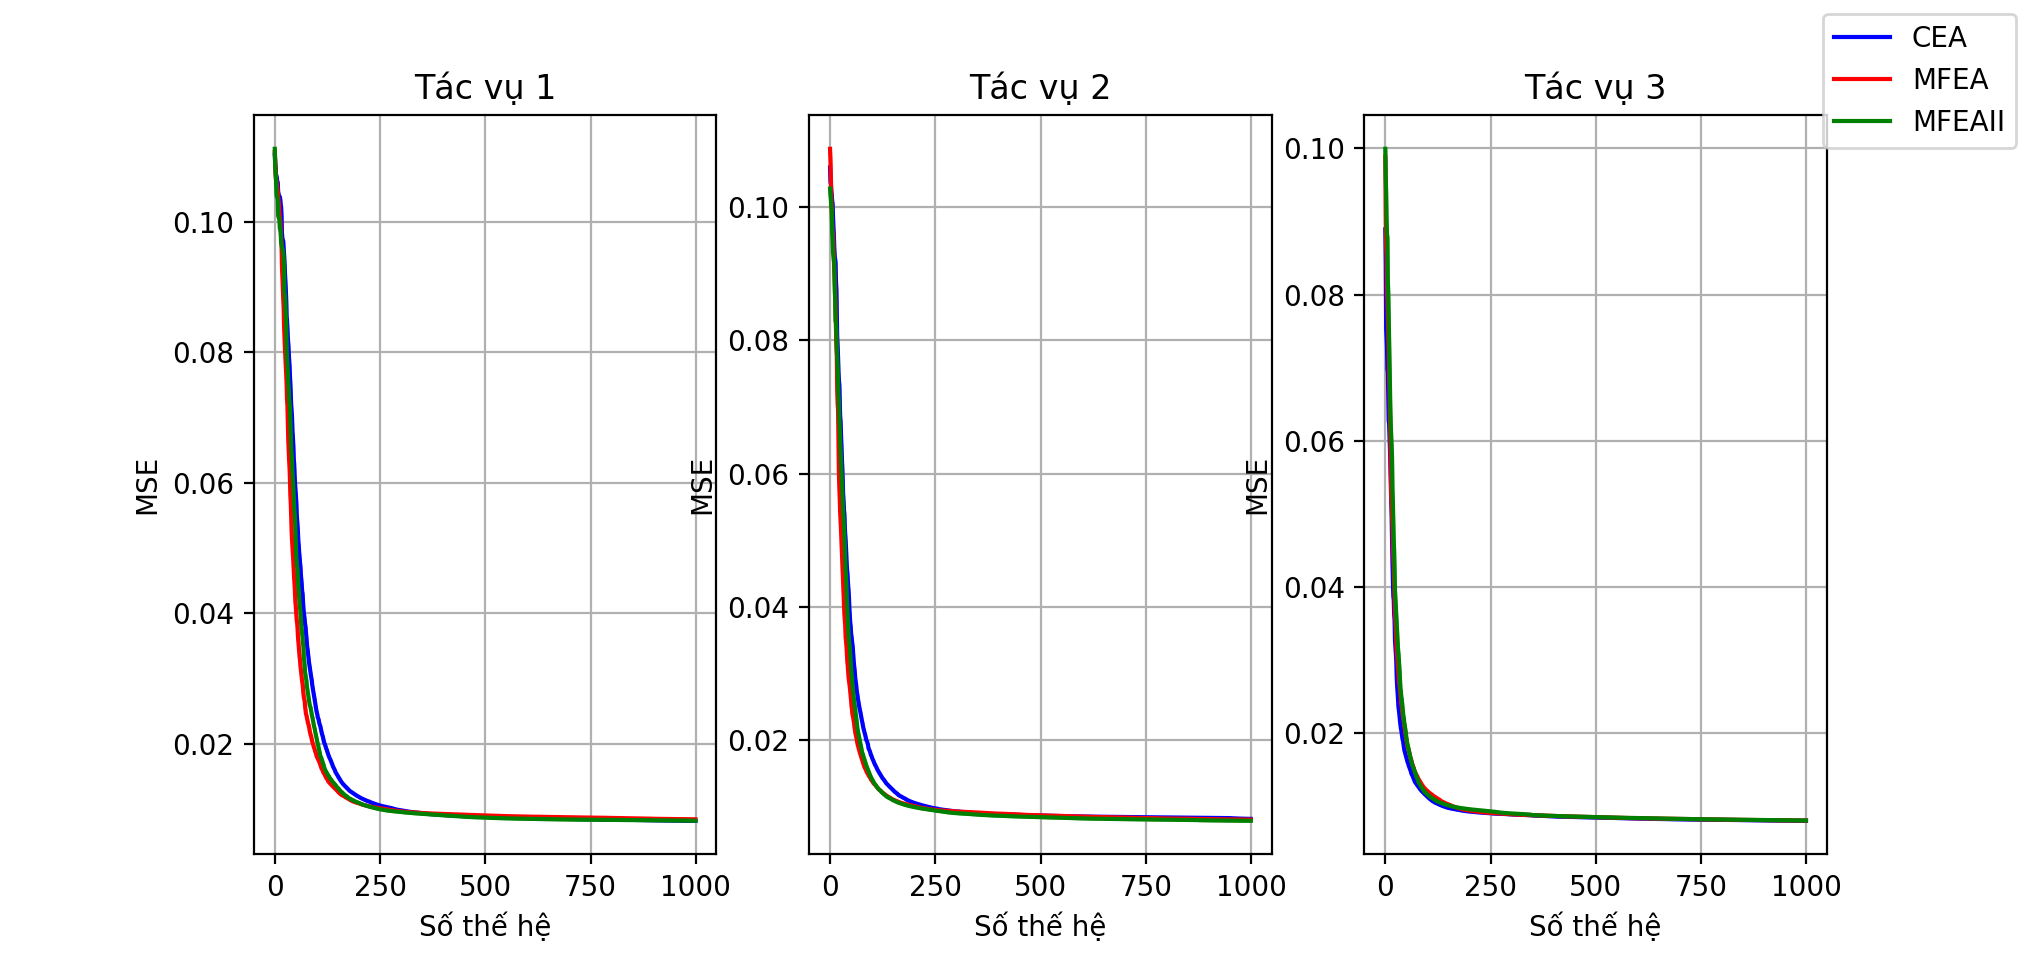
\includegraphics[width=\textwidth,height=\textheight,keepaspectratio]{thesis/images/results/uci/br_task.png}}
    \scalebox{.7}{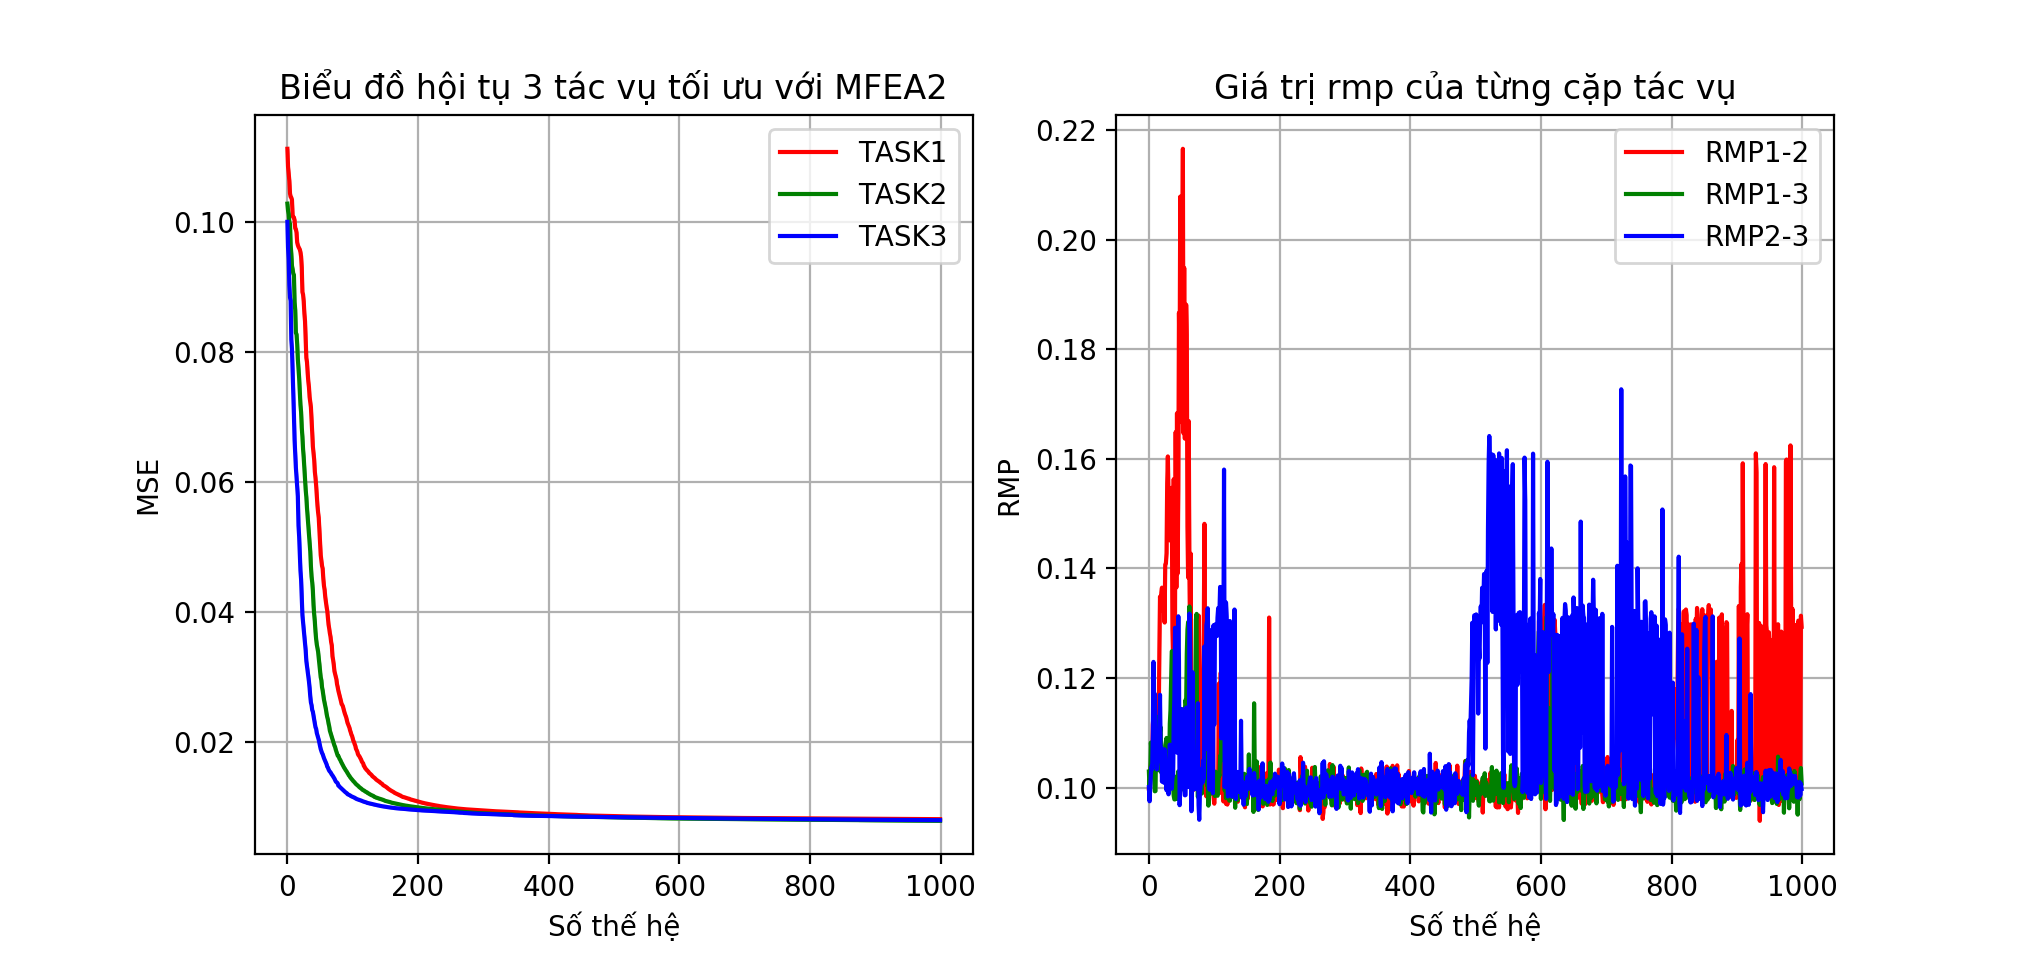
\includegraphics[width=\textwidth,height=\textheight,keepaspectratio]{thesis/images/results/uci/br_rmp.png}}
    \caption{Biểu đồ hội tụ bài BreastCancer khác độ sâu}
    \label{fig:br_mtl}
\end{figure}

\begin{figure}[h!]
    \centering
    \scalebox{.7}{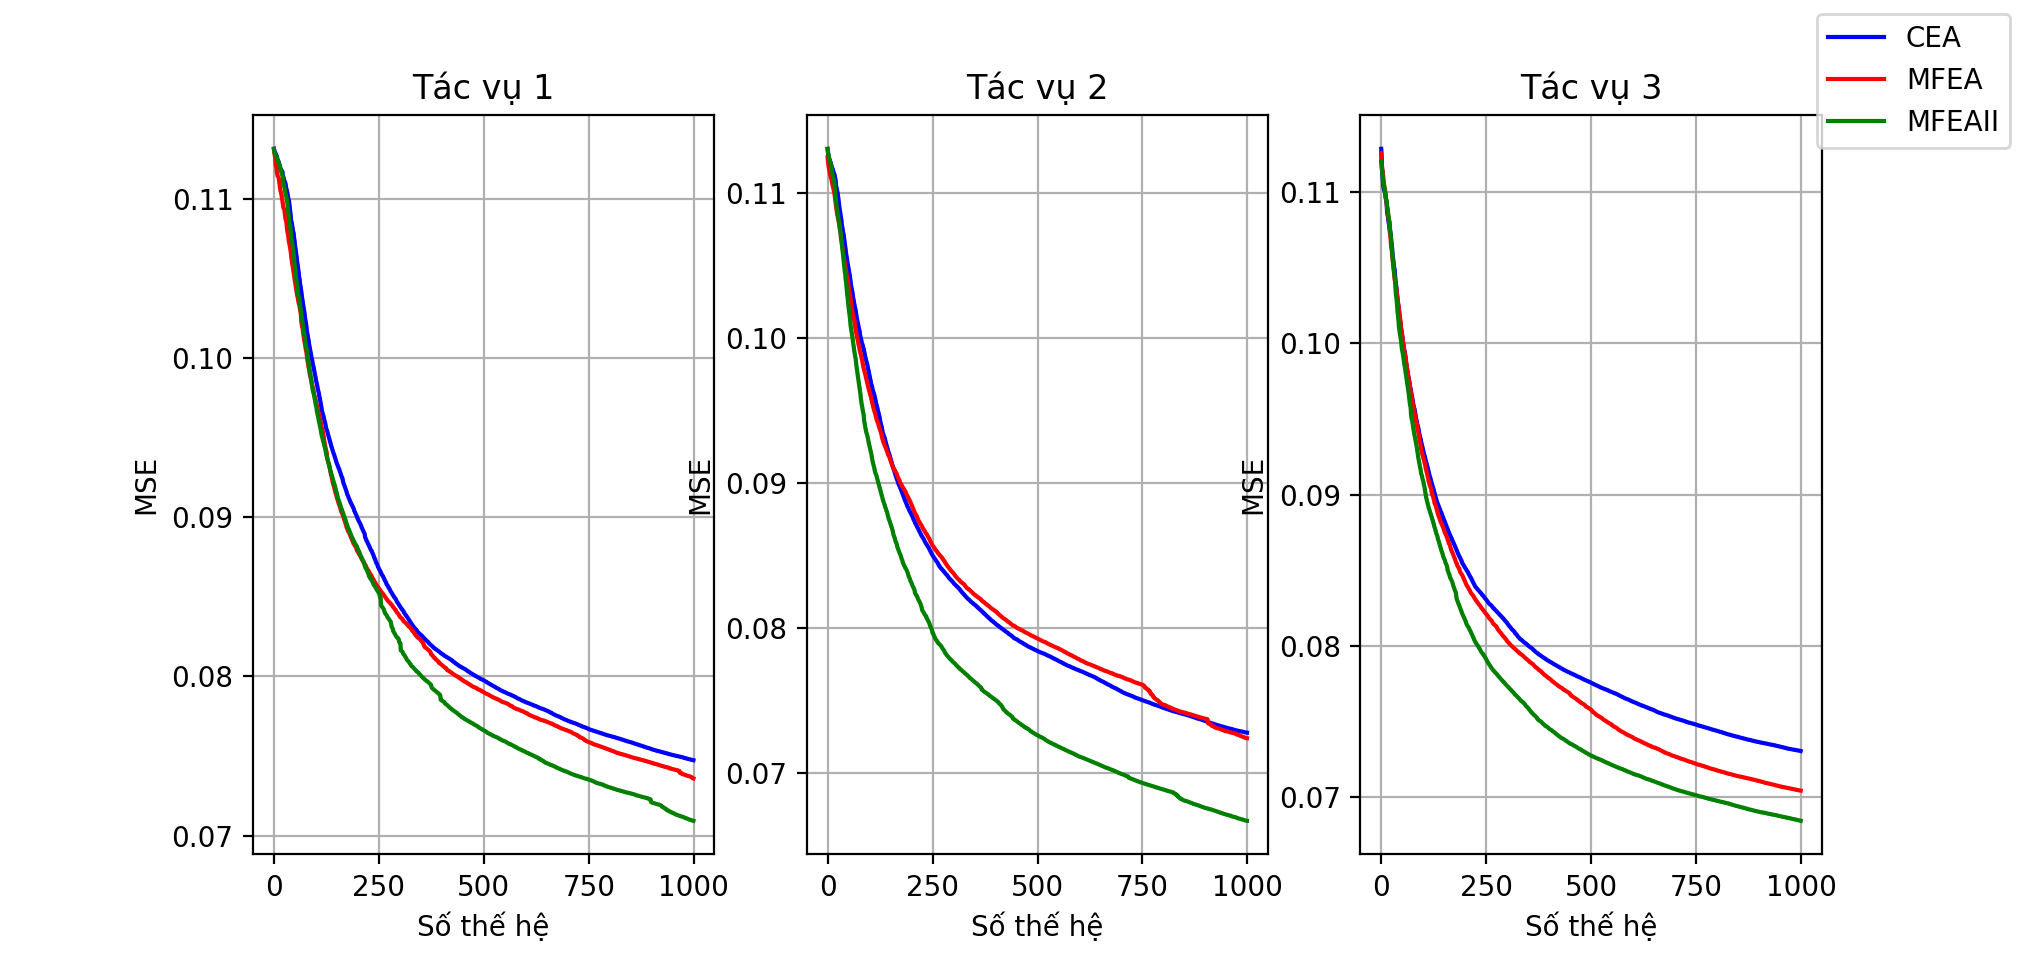
\includegraphics[width=\textwidth,height=\textheight,keepaspectratio]{thesis/images/results/uci/tt_task.png}}
    \scalebox{.7}{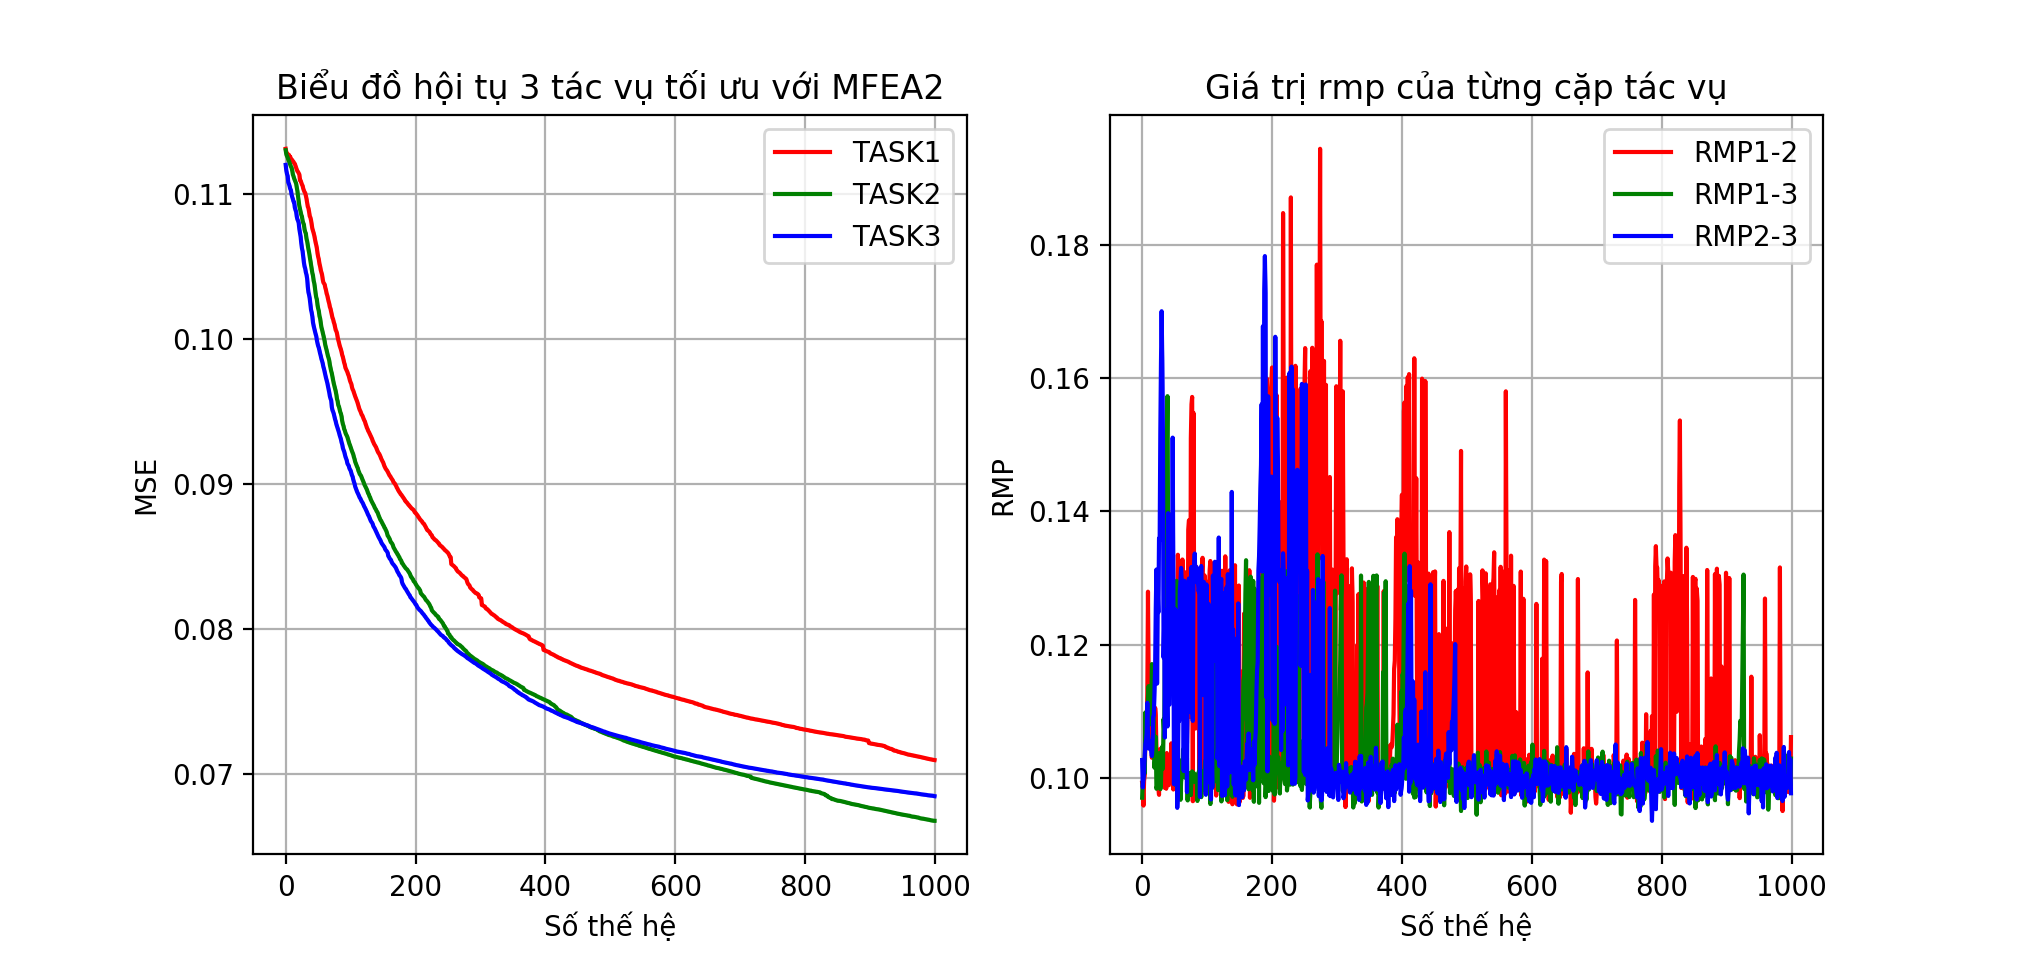
\includegraphics[width=\textwidth,height=\textheight,keepaspectratio]{thesis/images/results/uci/tt_rmp.png}}
    \caption{Biểu đồ hội tụ bài Tictactoe khác độ sâu}
    \label{fig:br_mtl}
\end{figure}
\pagebreak

\subsection{Kết quả huấn luyện trên các môi trường học tăng cường}
% \begin{table}
%     \caption{Mô hình học tăng cường khác môi trường}
%     \begin{center}
%     \begin{tabular}{|c|c|c|c|c|c|}
%     \hline
%     \multirow{1}{*}{\textbf{Trọng lực}} &
%     \multirow{1}{*}{\textbf{Method}} & \multicolumn{1}{c|}{\textbf{Cao nhất}} & {\textbf{Thấp nhất}} & \multicolumn{1}{c|}{\textbf{Trung Bình}} & \multicolumn{1}{c|}{\textbf{Độ lệch}} \\ \hline
%     \multirow{3}{*} 
%     {Trọng lực=1.0} &
%     CEA & $71$ & $4$ & $28.86$ & $17.16$ \\
%     & MFEAI & $\mathbf{129}$ & $17$ &$46.71$ & $20.36$  \\
%     & MFEAII & $84$ & $15$ & $\mathbf{52.81}$  &$15.45$\\\hline
%     \multirow{3}{*} 
%     {Trọng lực=1.98} &
%     CEA & $382$ & $7$ &$174.86$ & $113.79$ \\
%     & MFEAI  & $\mathbf{546}$ & $98$ & $\mathbf{319.86}$ & $95.34$ \\
%     & MFEAII & $517$ & $\mathbf{131}$ &$311.38$ & $106.76$ \\\hline
%     \multirow{3}{*} 
%     {Trọng lực=2.96} &
%     CEA & $272$ & $1$ &$97.9$ & $83.07$ \\
%     & MFEAI  & $\mathbf{349}$ & $\mathbf{140}$ & $\mathbf{222.81}$ & $52.07$ \\
%     & MFEAII & $322$ & $103$ &$212.38$ & $52.74$ \\\hline
%     \multirow{3}{*} 
%     {Trọng lực=3.94} &
%     CEA & $227$ & $2$ &$69.24$ & $56.64$ \\
%     & MFEAI  & $\mathbf{217}$ & $\mathbf{95}$ & $\mathbf{142.86}$ & $27.4$ \\
%     & MFEAII & $190$ & $76$ &$140.38$ & $27.78$ \\\hline
%     \multirow{3}{*} 
%     {Trọng lực=4.92} &
%     CEA & $95$ & $2$ & $25.48$ & $25.78$  \\
%     & MFEAI  & $\mathbf{181}$ & $\mathbf{54}$ & $90.86$ & $21.98$ \\
%     & MFEAII & $145$ & $44$ & $\mathbf{102.14}$ & $26.66$ \\\hline
%     \end{tabular}
%     \end{center}
    
%     \label{tab:result:nbit}
% \end{table}

\subsubsection{Bảng kết quả thực nghiệm - bài toán Acrobot}
\begin{table} [H]
    \begin{center}
    \caption{Kết quả huấn luyện các tác vụ cho bài toán Acrobot}

    \scalebox{0.9}{\begin{tabular}{|c|c|c|c|c|c|}
    \hline
    \multirow{1}{*}{\textbf{Thuật toán}} & \multicolumn{1}{c|}{\textbf{Tác vụ 1}} & \multicolumn{1}{c|}{\textbf{Tác vụ 2}} & \multicolumn{1}{c|}{\textbf{Tác vụ 3}} & \multicolumn{1}{c|}{\textbf{Tác vụ 4}} & \multicolumn{1}{c|}{\textbf{Tác vụ 5}} \\ \hline
    CEA & $-100 \pm 4.53$ & $-109.47 \pm 2.38$ & $-108.77 \pm 4.38$ & $-113.17 \pm 1.86$ & $-117.23 \pm 4.28$  \\
    MFEAI &  $-100 \pm 4.75$ & $\mathbf{-106.7 \pm 0.78}$ & $\mathbf{-108.3 \pm 4.47}$ & $-112.0 \pm 2.62$ & $-117.03 \pm 4.52$ \\
    MFEAII & $\mathbf{-100 \pm 4.7}$ & $-107.8 \pm 1.17$ & $-108.6 \pm 4.34$ & $\mathbf{-113.07 \pm 2.29}$ & $\mathbf{-116.9 \pm 4.09}$  \\\hline
    \end{tabular}}
    \end{center}
    \label{tab:result:acrobot}
\end{table}


\subsubsection{Biểu đồ hội tụ - bài toán Acrobot}
\begin{figure}[h!]
    \centering
    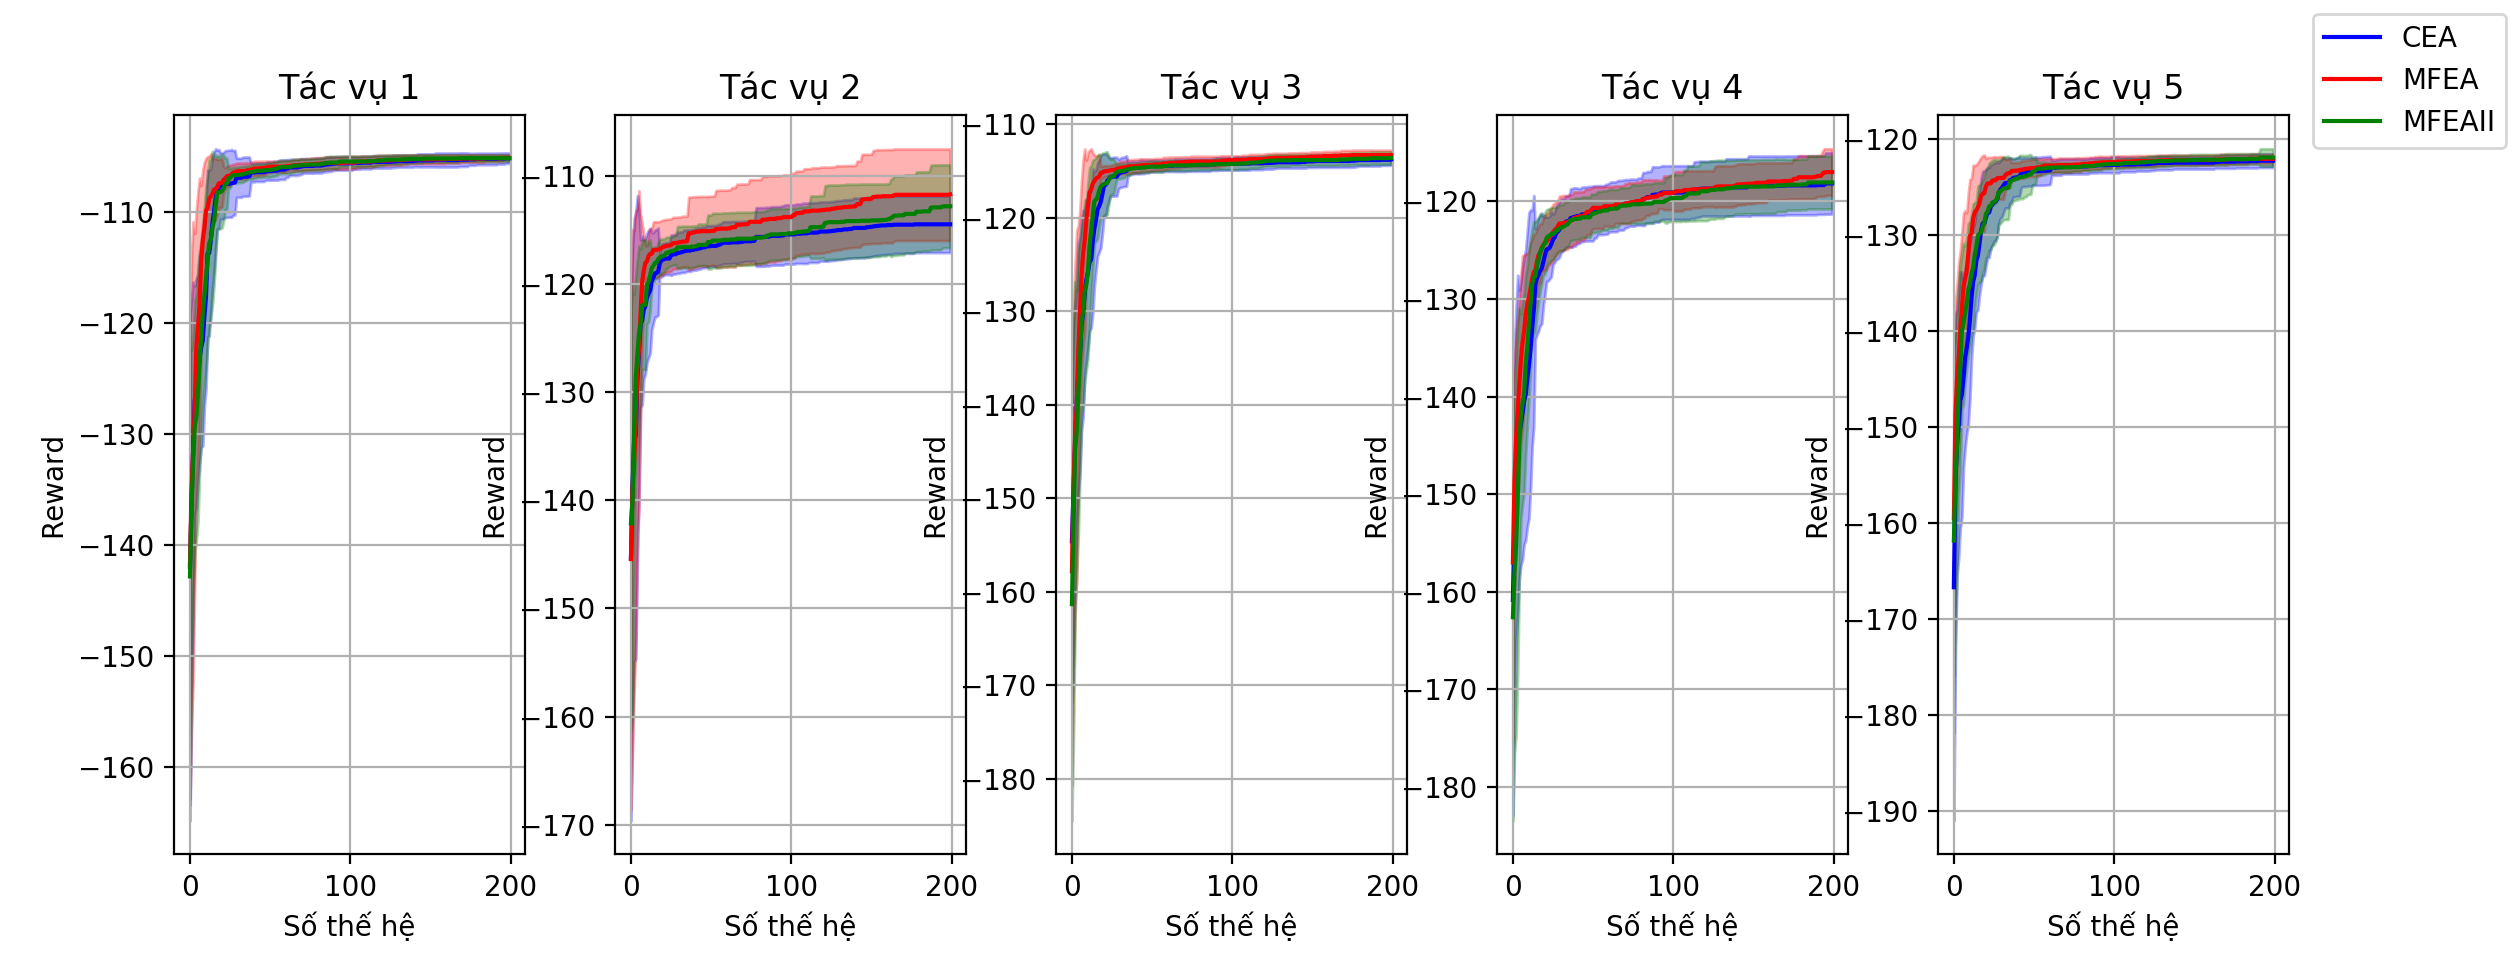
\includegraphics[width=\textwidth,height=\textheight,keepaspectratio]{thesis/images/results/rl/acrobot_conv.png}
    \caption{Biểu đồ hội tụ các tác vụ cho bài toán Acrobot}
    \label{fig:Acrobot_conv}
\end{figure}

\subsubsection{So sánh mức độ tập trung kết quả cuối cùng - bài toán Acrobot}
\begin{figure}[h!]
    \centering
    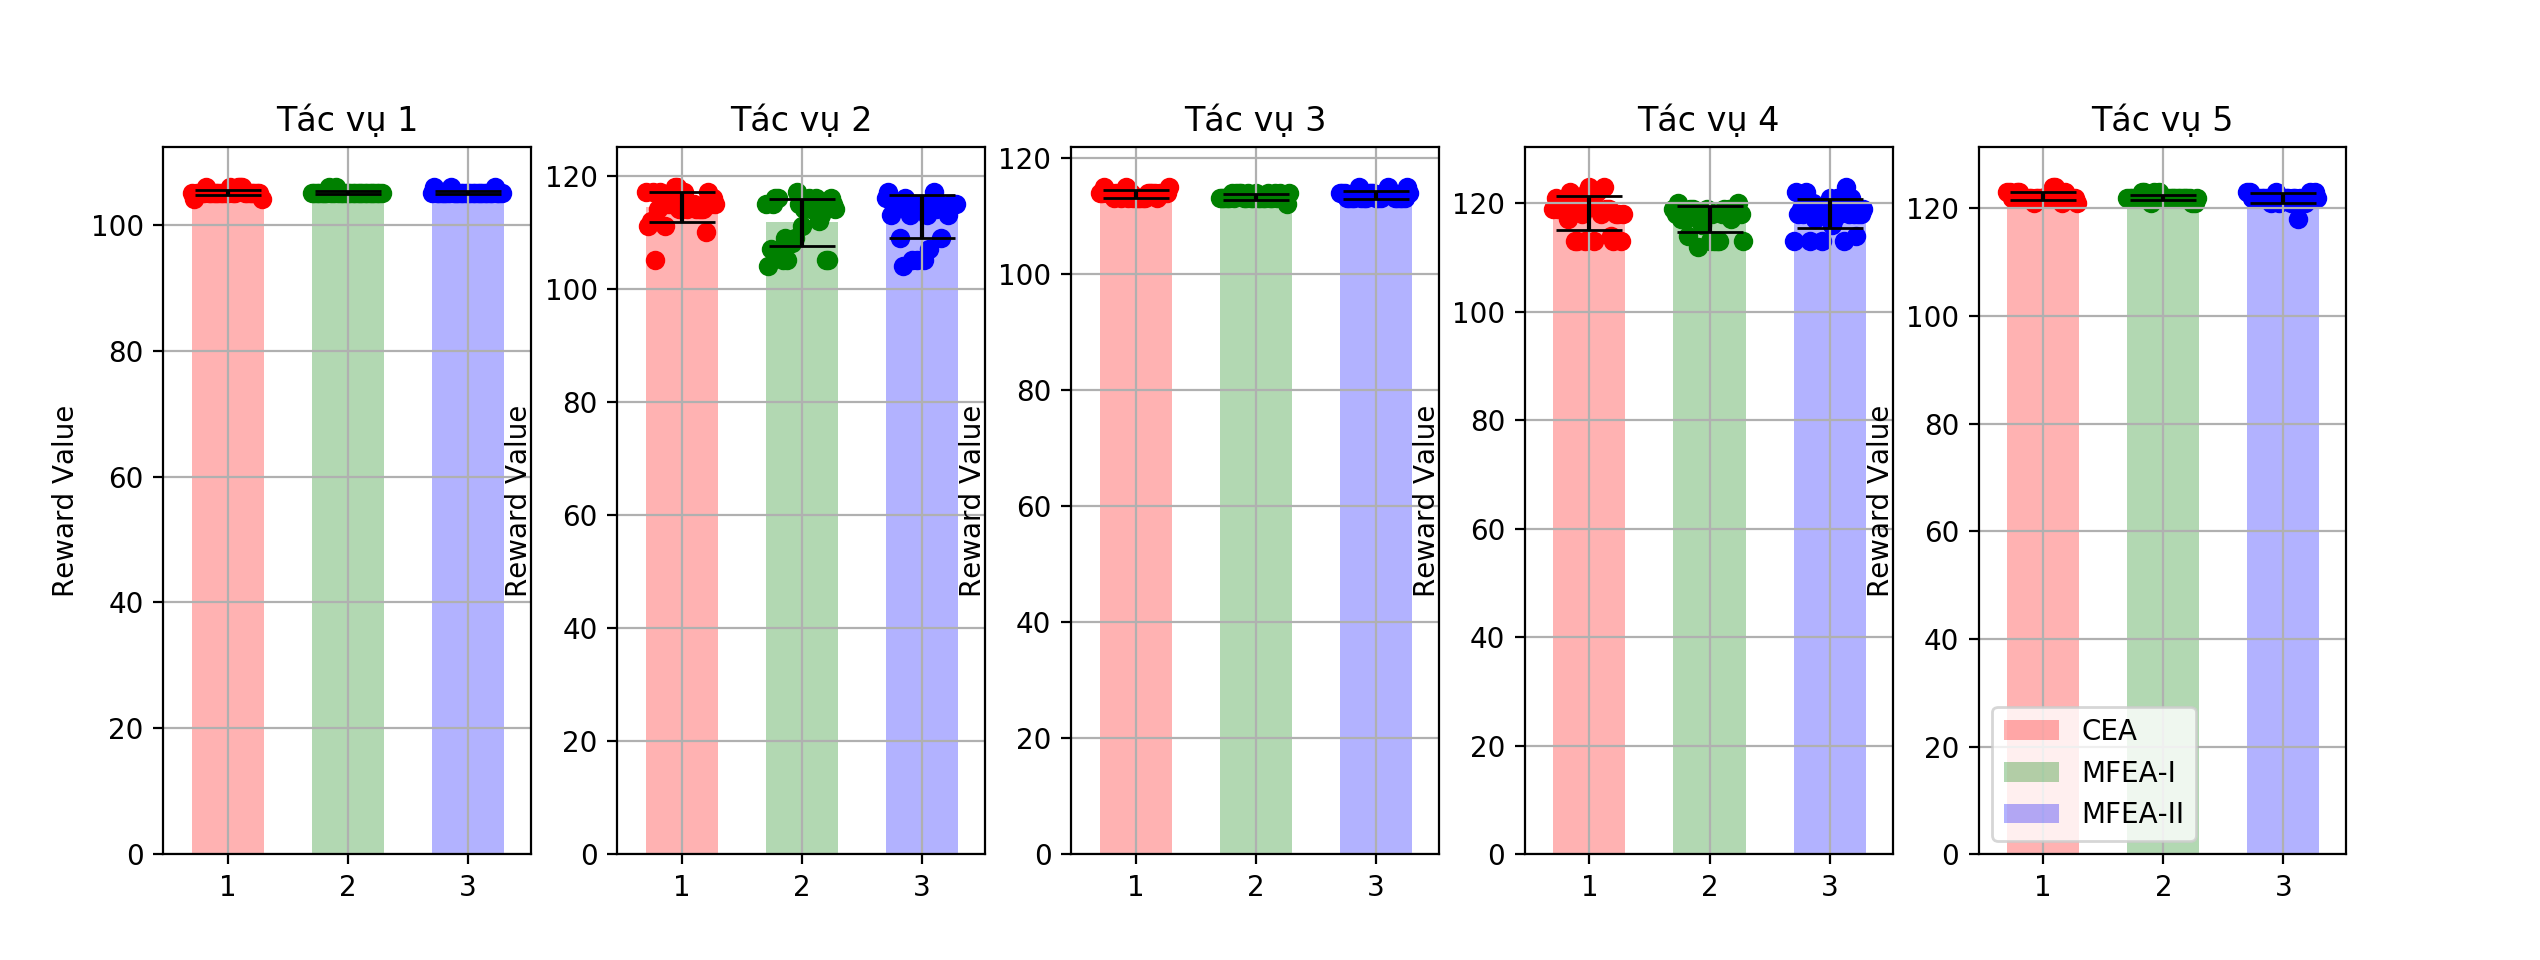
\includegraphics[width=\textwidth,height=\textheight,keepaspectratio]{thesis/images/results/rl/acrobot_final.png}
    \caption{Biểu đồ so sánh mức độ tập trung kết quả cuối cùng cho bài toán Acrobot (khi so sánh trị tuyệt đối của kết quả)}
    \label{fig:Acrobot}
\end{figure}


\subsubsection{Bảng kết quả thực nghiệm - bài toán PixelCopter}
\begin{table} [h!]
    \begin{center}
    \caption{Kết quả huấn luyện các tác vụ cho bài toán PixelCopter}

    \scalebox{0.9}{\begin{tabular}{|c|c|c|c|c|c|}
    \hline
    \multirow{1}{*}{\textbf{Thuật toán}} & \multicolumn{1}{c|}{\textbf{Tác vụ 1}} & \multicolumn{1}{c|}{\textbf{Tác vụ 2}} & \multicolumn{1}{c|}{\textbf{Tác vụ 3}} & \multicolumn{1}{c|}{\textbf{Tác vụ 4}} & \multicolumn{1}{c|}{\textbf{Tác vụ 5}} \\ \hline
    CEA & $101.97 \pm 26.15$ & $104.6 \pm 23.16$ & $96.83 \pm 22.74$ & $96.67 \pm 28.27$ & $93.47 \pm 19.09$ \\
    MFEAI & $124.47 \pm 32.08$ & $125.93 \pm 31.4$ & $123.43 \pm 24.86$ & $122.33 \pm 23.08$ & $120.37 \pm 30.36$  \\
    MFEAII & $\mathbf{133.57 \pm 28.29}$ & $\mathbf{132.03 \pm 33.31}$ & $\mathbf{132.73 \pm 26.93}$ & $\mathbf{129.0 \pm 22.93}$ & $\mathbf{135.4 \pm 30.11}$ \\\hline
    \end{tabular}}
    \end{center}
    \label{tab:result:pixelcopter}
\end{table}


\subsubsection{Biểu đồ hội tụ - bài toán PixelCopter}
\begin{figure}[h!]
    \centering
    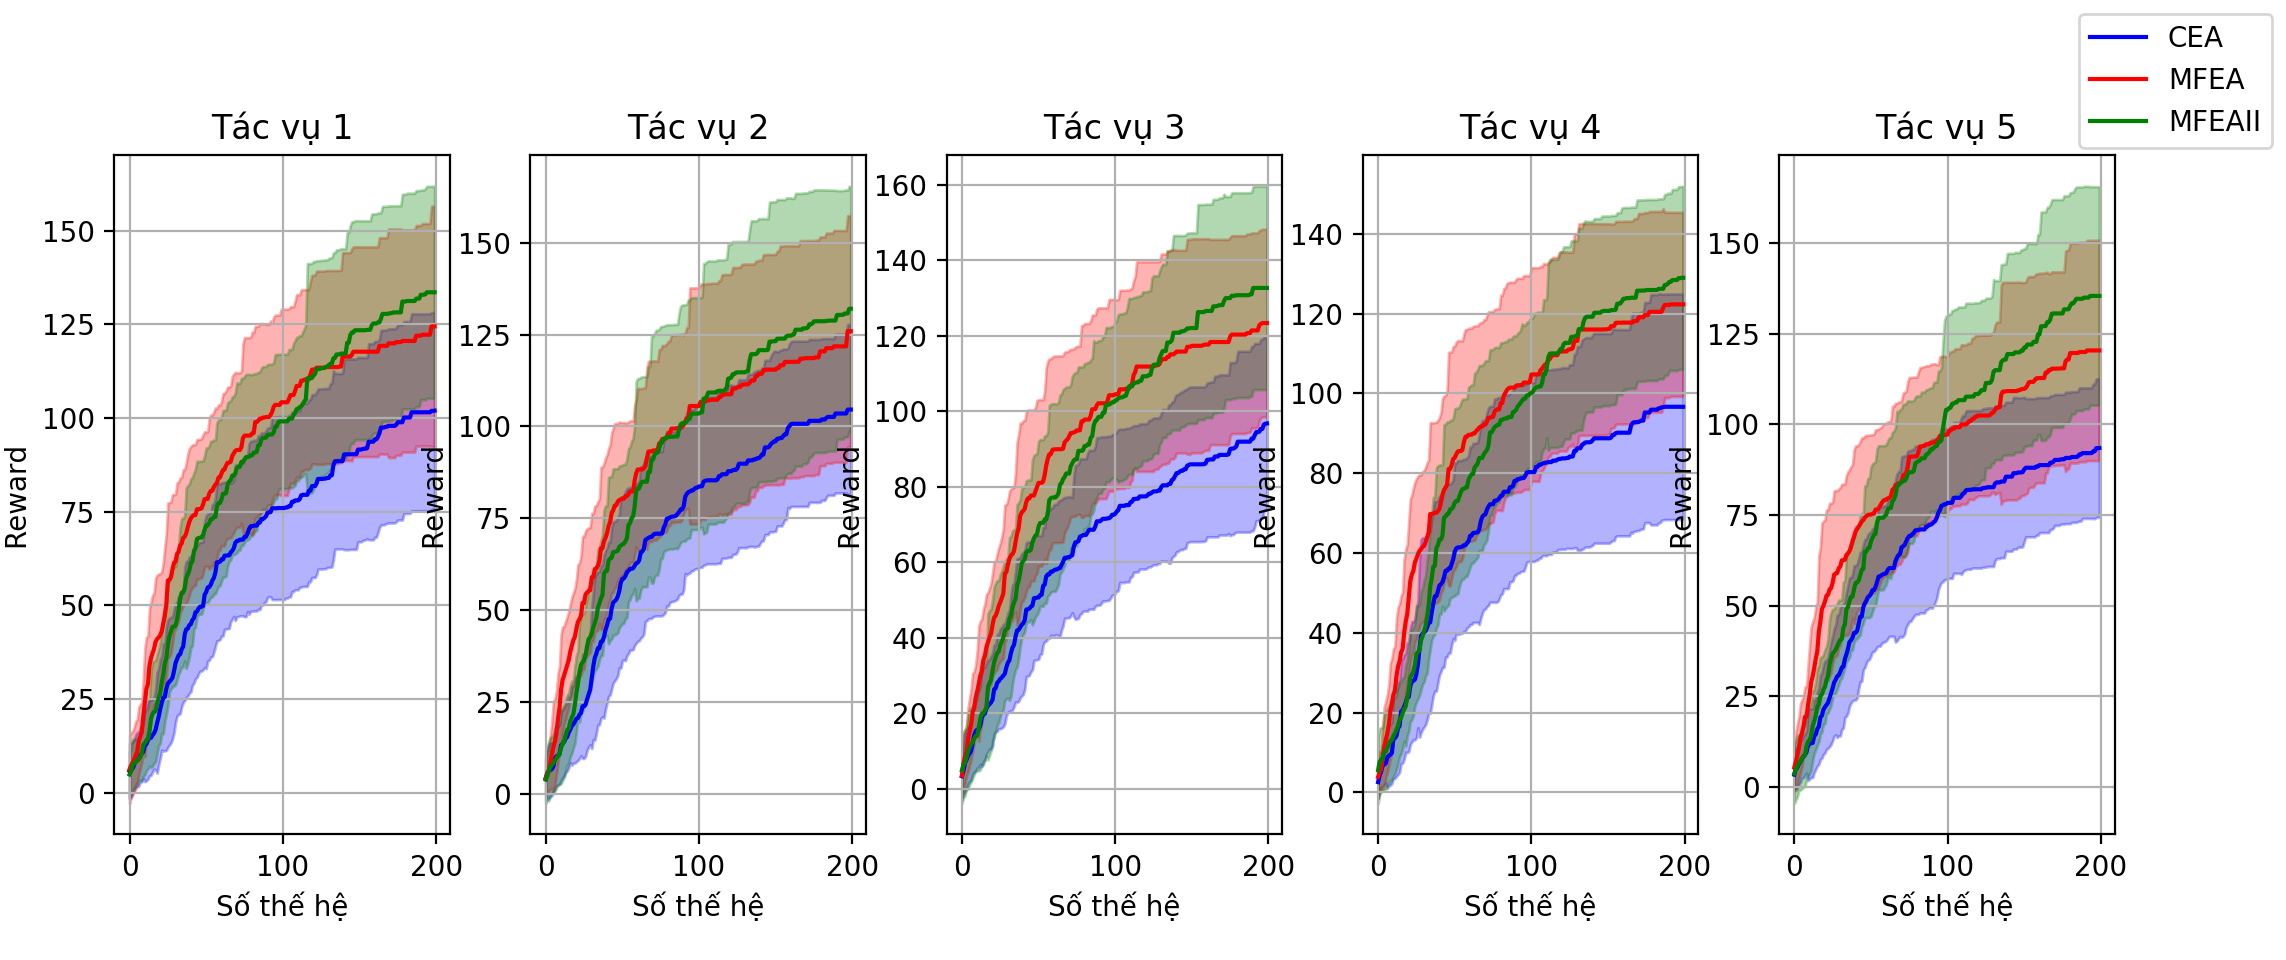
\includegraphics[width=\textwidth,height=\textheight,keepaspectratio]{thesis/images/results/rl/pixcelcopter_conv.png}
    \caption{Biểu đồ hội tụ các tác vụ cho bài toán PixelCopter}
    \label{fig:PixelCopter_conv}
\end{figure}

\subsubsection{So sánh mức độ tập trung kết quả cuối cùng - bài toán PixelCopter}
\begin{figure}[h!]
    \centering
    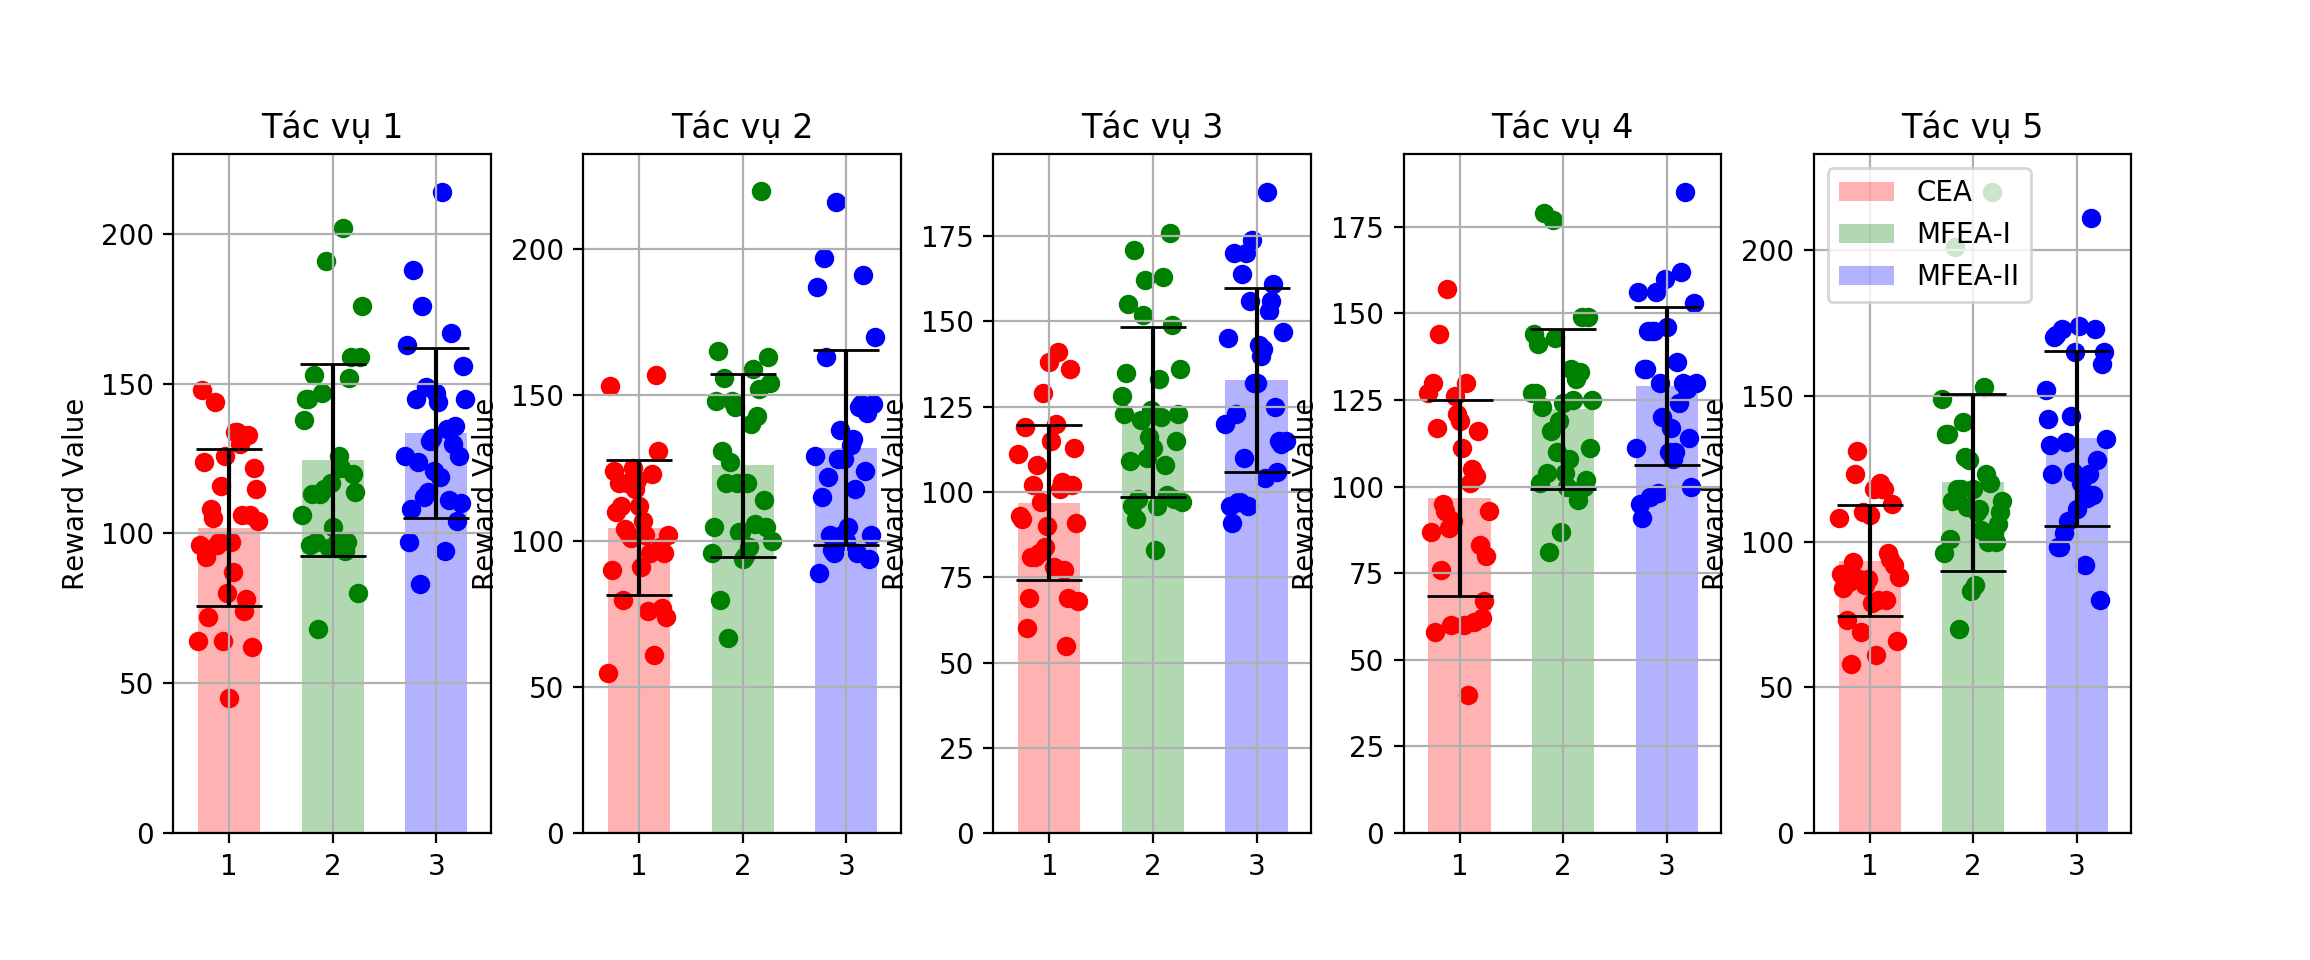
\includegraphics[width=\textwidth,height=\textheight,keepaspectratio]{thesis/images/results/rl/pixelcopter_final.png}
    \caption{Biểu đồ so sánh mức độ tập trung kết quả cuối cùng cho bài toán PixelCopter}
    \label{fig:PixelCopter}
\end{figure}
\subsubsection{Bảng kết quả thực nghiệm - bài toán FlappyBird}
\begin{table} [H]
    \begin{center}
    \caption{Kết quả huấn luyện các tác vụ cho bài toán FlappyBird}

    \scalebox{0.9}{\begin{tabular}{|c|c|c|c|c|c|}
    \hline
    \multirow{1}{*}{\textbf{Thuật toán}} & \multicolumn{1}{c|}{\textbf{Tác vụ 1}} & \multicolumn{1}{c|}{\textbf{Tác vụ 2}} & \multicolumn{1}{c|}{\textbf{Tác vụ 3}} & \multicolumn{1}{c|}{\textbf{Tác vụ 4}} & \multicolumn{1}{c|}{\textbf{Tác vụ 5}} \\ \hline
    CEA & $25.9 \pm 17.57$ & $219.1 \pm 151.39$ & $101.8 \pm 88.65$ & $78.77 \pm 62.43$ & $24.63 \pm 23.62$ \\
    MFEAI & $47.43 \pm 17.97$ & $\mathbf{319.83 \pm 118.9}$ & $\mathbf{217.87 \pm 48.57}$ & $142.9 \pm 26.86$ & $90.17 \pm 20.69$ \\
    MFEAII & $\mathbf{50.93 \pm 16.47}$ & $314.07 \pm 116.25$ & $214.83 \pm 51.96$ & $\mathbf{145.47 \pm 26.72}$ & $\mathbf{105.33 \pm 26.12}$ \\\hline
    \end{tabular}}
    \end{center}
    \label{tab:result:pixelcopter}
\end{table}


\subsubsection{Biểu đồ hội tụ - bài toán FlappyBird}
\begin{figure}[h!]
    \centering
    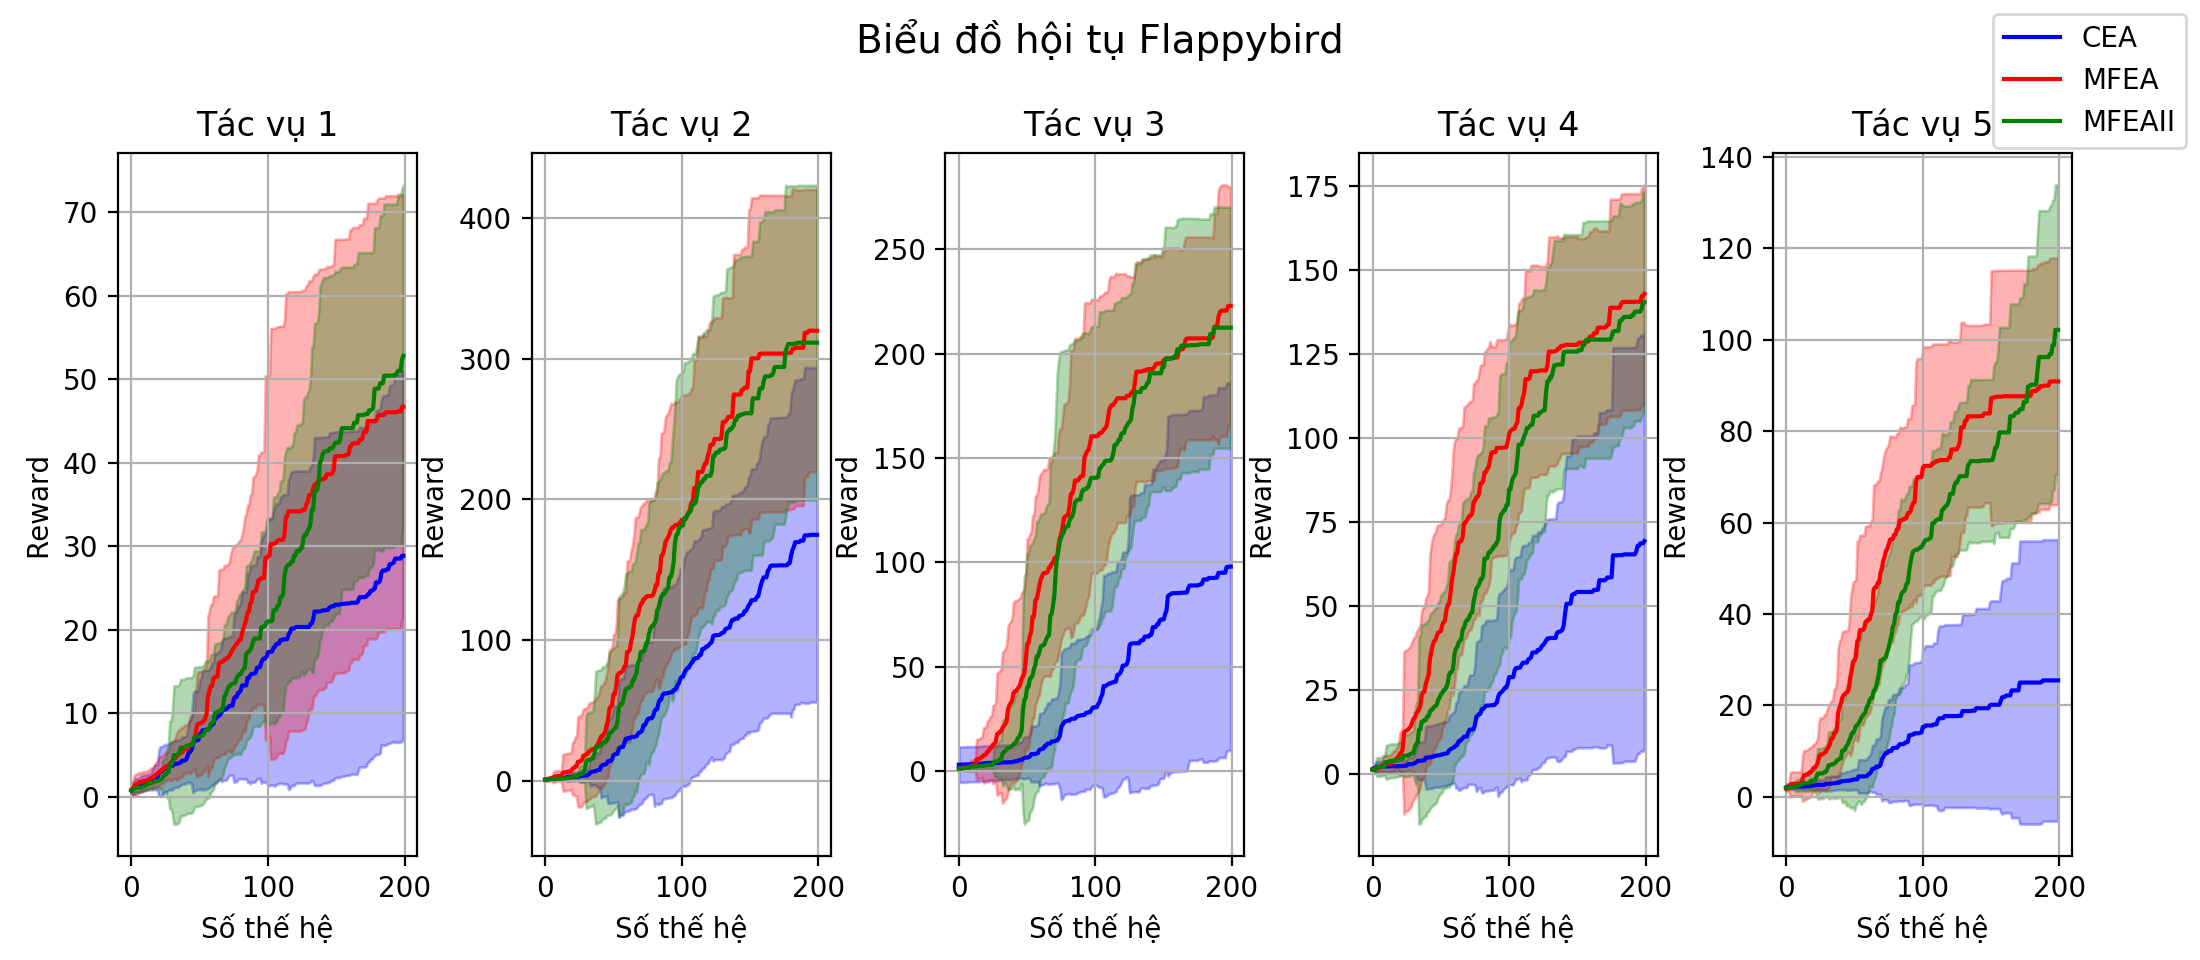
\includegraphics[width=\textwidth,height=\textheight,keepaspectratio]{thesis/images/results/rl/flappybird_conv.png}
    \caption{Biểu đồ hội tụ các tác vụ cho bài toán FlappyBird}
    \label{fig:FLP_conv}
\end{figure}

\subsubsection{So sánh mức độ tập trung kết quả cuối cùng - bài toán FlappyBird}
\begin{figure}[h!]
    \centering
    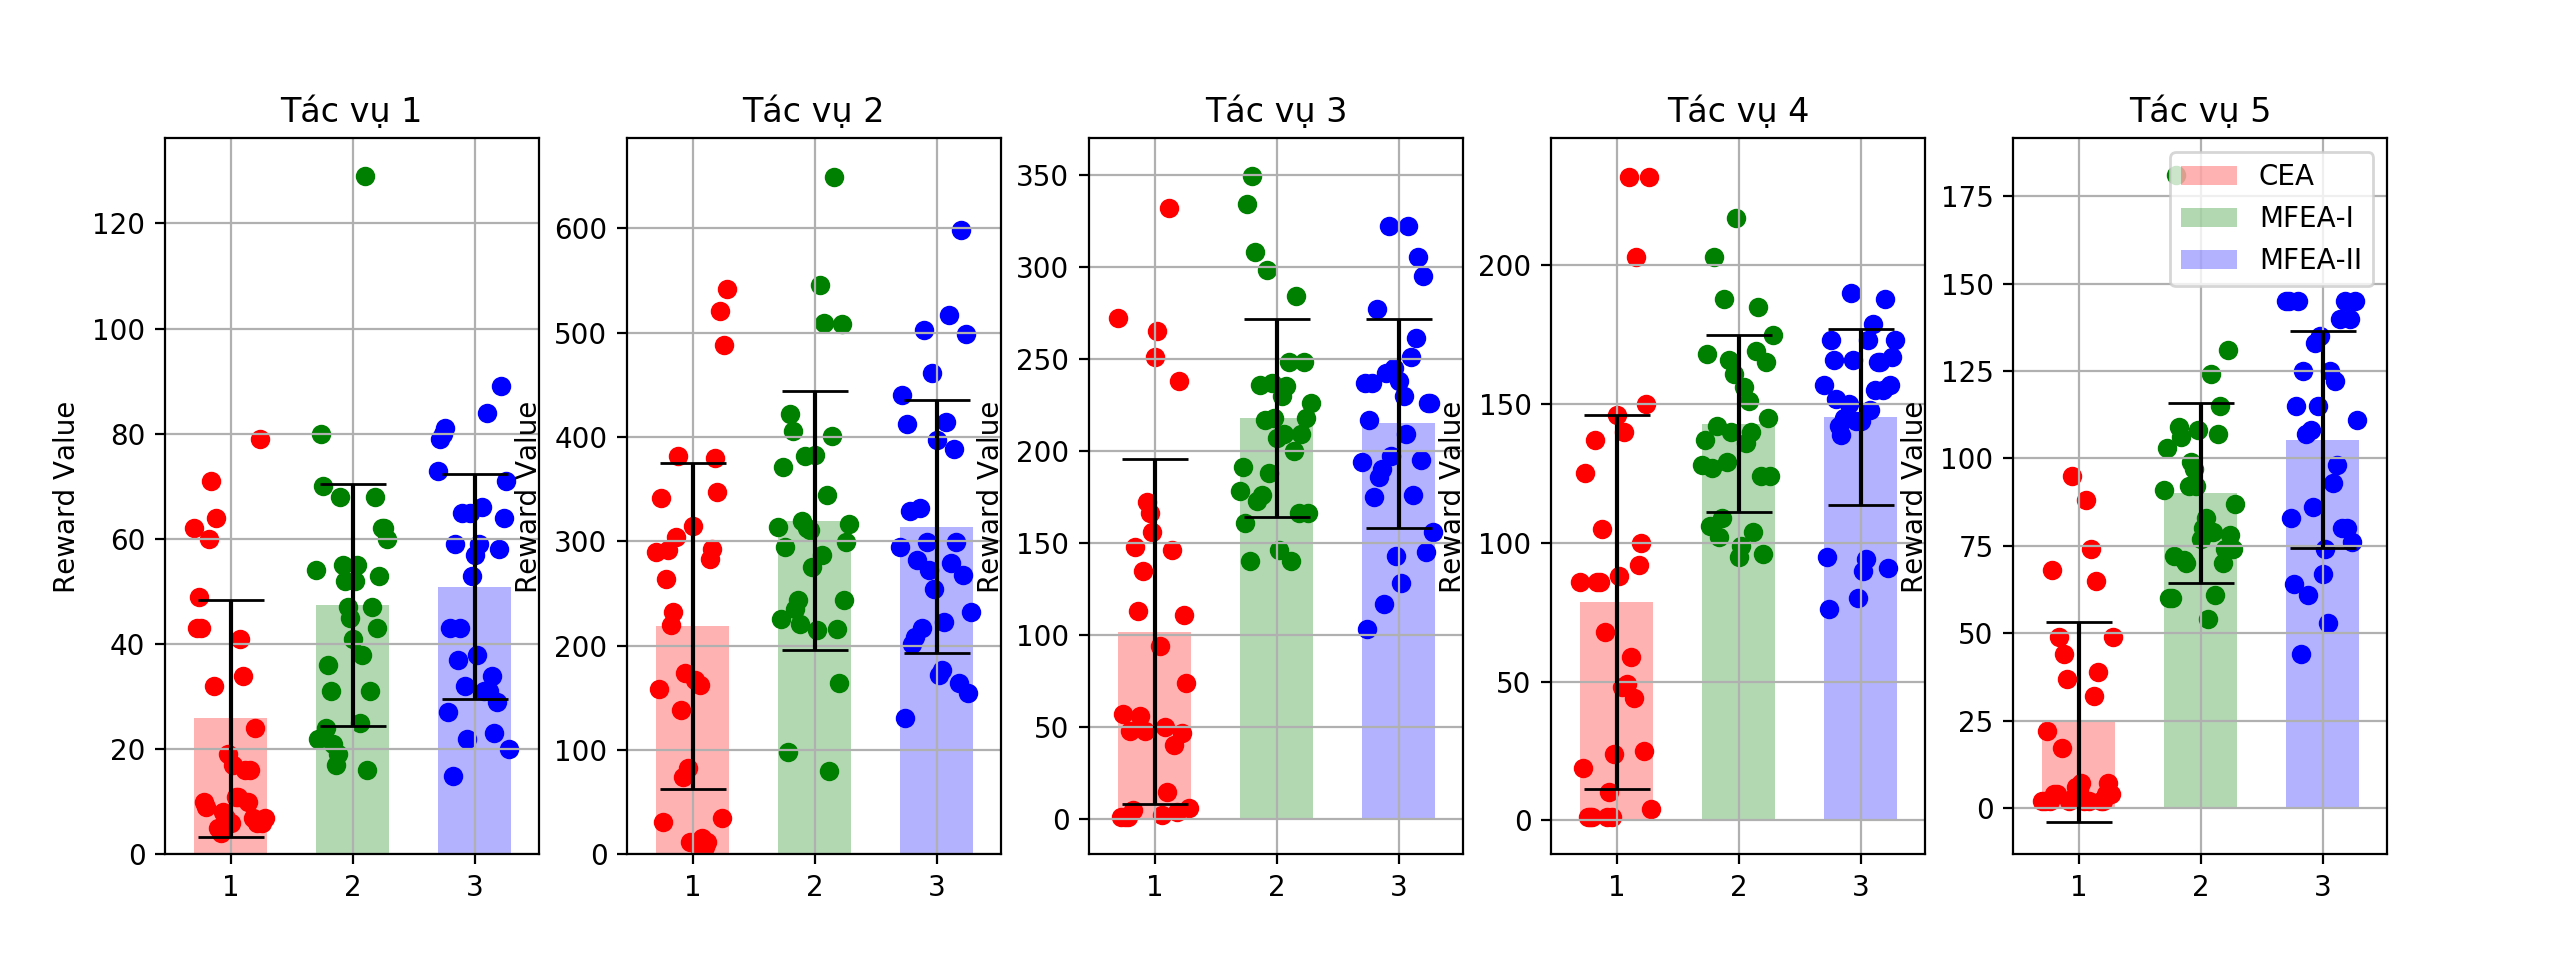
\includegraphics[width=\textwidth,height=\textheight,keepaspectratio]{thesis/images/results/rl/flappybird_final.png}
    \caption{Biểu đồ so sánh mức độ tập trung kết quả cuối cùng cho bài toán FlappyBird}
    \label{fig:FLP}
\end{figure}

\pagebreak
\section{Nhận xét và bàn luận}
\subsection{Bài toán huấn luyện nhiều ANN khác cấu trúc}

Kết quả thực nghiệm chỉ rõ ưu điểm của cách tiếp cận của tiến hóa đa nhiệm trên tất cả các bộ dữ liệu thực nghiệm. Giải thuật CEA thể hiện không tốt trên tất cả các bài \emph{n-bit} và các bộ dữ liệu thực tế so với cách tiếp cận bằng tiến hóa đa nhiệm. Điều này có thể lý giải bởi với các bài toán có cấu trúc gần tương đồng với nhau việc trao đổi tri thức giữa các tác vụ giúp tăng tốc độ tối ưu trên từng tác vụ. Và khi so sánh giữa các giải thuật tiến hóa đa nhiệm với nhau thì MFEA-II thể hiện sự vượt trội so với MFEA-I nhờ ưu thế có thể xác định được mức độ chia sẻ tri thức phù hợp tại từng thời điểm. Các tác vụ được tối ưu hóa bởi MFEA-II có tốc độ nhanh hơn so với các thuật toán khác trên tất cả các tác vụ.

\subsubsection{Mạng cùng độ sâu}
Trong bài thực nghiệm ANN cùng độ sâu thuật toán MFEA-II tốt hơn so với CEA $100\%$ (8/8) số bộ dữ liệu, so với MFEA-I là $75\%$ số bộ dữ liệu (6/8). Với các bộ dữ liệu MFEA-II trội hơn thì xét về mức độ cải tiến, so với CEA là $10 \sim 12\%$, so với MFEA là $6 \sim 8\%$. Trên một số bài như trong hình \ref{fig:10bit_2layer} thì MFEA-II và MFEA-I có kết quả tương dương nhau tất cả các tác vụ. Có thể lý giải rằng với những bộ này mức độ tương đồng trung bình giữa các tác vụ là lớn việc dẫn tới việc tối ưu bằng MFEA-II hay MFEA-I không có nhiều khác biệt. Tuy nhiên MFEA-II vẫn có thể coi là tốt hơn nếu nhìn trên góc độ tốc độ hội tụ của thuật toán.

\subsubsection{Mạng khác độ sâu}
Trong bài thực nghiệm ANN cùng khác sâu thuật toán MFEA-II tốt hơn so với CEA và MFEA-I $100\%$ (3/3) số bộ dữ liệu. Xét về mức độ cải tiến, so với CEA là $12 \sim 15\%$, so với MFEA là $5 \sim 7\%$. Cá biệt trong hình \ref{fig:8bit_multilayer} thì mặc dù tính số lượng trên 3 tác vụ MFEA-II đem lại kết quả tốt hơn nhưng với tác vụ thứ 3, MFEA-II có kết quả kém hơn so với MFEA-I và CEA thông thường. Điều này có thể lý giải bởi ở các mạng sâu khác nhau về số lớp, lượng tham số chia sẻ chung giữa các cấu hình là thấp hơn, do đó các phép lai ghép đa nhiệm ít tỏ ra ưu thế của mình và chất lượng lời giải của MFEA.

Khi so sánh hiệu quả của mạng 2 lớp rộng với mạng nhiều lớp hơn nhưng sâu (3, 4, 5 lớp) như Hình V.1 với Hình V.7 hay trong Hình V.3 với Hình V.9, ..., ta thấy rằng các mạng sâu và hẹp có hiệu quả tốt tương đương với mạng nông và rộng hơn dù cho các mạng sâu hẹp ít tham số hơn nhiều. Điều này có được là do việc tăng độ sâu của mạng giúp tăng độ phức tạp của hàm xấp xỉ biểu diễn nên khớp dữ liệu học tốt hơn.

Tổng kết thực nghiệm, ta thấy rõ hiệu quả của chất lượng mạng ANN học bởi các phương pháp tiếp cận dựa trên MFEA đặc biệt là MFEA-II. Tuy nhiên, để có được chất lượng lời giải tất MFEA-II phải trả giá về mặt thời gian. Trung bình thời gian thực nghiệm trên một bộ dữ liệu của MFEA-II sẽ nhiều gấp 3 lần so với CEA và 2.5 lần nếu so với MFEA-I.

\subsection{Bài toán huấn luyện nhiều mô hình học tăng cường}

Với bộ dữ liệu thực nghiệm đơn giản Acrobot, các thuật toán đều có thể giải ngay ở những thế hệ đầu tiên, và mức độ chênh lệch giữa tốc độ hội tụ và mức độ tập trung kết quả cuối cùng cũng không thể hiện rõ sự chênh lệch giữa từng giải thuật.
Với bộ dữ liệu thực nghiệm phức tạp hơn như PixelCopter, FlappyBird, kết quả thực nghiệm trên các bộ dữ liệu học tăng cường chỉ rõ ưu điểm của cách tiếp cận của tiến hóa đa nhiệm. Về cả 3 mục tiêu chí so sánh giữa kết quả thực nghiệm, tốc độ hội tụ, mức độ phân bố kết quả cuối cùng thì kết quả được đưa ra bởi các thuật toán tiến hóa đa nhiệm đều vượt trội như trong hình \ref{fig:FLP_conv}, \ref{fig:FLP}, \ref{fig:PixelCopter_conv} và \ref{fig:PixelCopter}. Điều này có thể lý giải bởi với các bài toán có cấu trúc gần tương đồng với nhau việc trao đổi tri thức giữa các tác vụ giúp tăng tốc độ tối ưu trên từng tác vụ.
Và khi so sánh giữa các giải thuật tiến hóa đa nhiệm với nhau thì MFEA-II thể hiện sự vượt trội so với MFEA-I nhờ ưu thế có thể xác định được mức độ chia sẻ tri thức phù hợp tại từng thời điểm.
\chapter{Kết quả thực nghiệm}
\label{chap:result}

\section{Cơ sở so sánh thuật toán tiến hóa}
Các thực nghiệm được thiết kế để chứng minh độ hiệu quả của MFEA-II trong bài toán huấn luyện nhiều mạng ANN khác cấu trúc và mô hình ANN biểu diễn mạng policy của RL. Nhằm đánh giá hiệu quả của giải thuật đề xuất áp dụng MFEA-II, đồ án thực nghiệm so sánh với các giải thuật tiến hóa, tiến hóa đa nhiệm thông thường là CEA và MFEA-I. 
\section{Các bộ thực nghiệm}
\subsection{Mạng neual khác cấu trúc}
\subsubsection{Bộ dữ liệu thực nghiệm}
Bài toán chính để thực nghiệm là bài toán n-bit. Bài toán có đầu vào là một chuỗi bit độ dài n, yêu cầu đầu ra là xác định số bit 1 trong dãy là chẵn hay lẻ. Trong [53], tác giả thực nghiệm với các bài toán 6-bit, 7-bit và 8-bit đối với các mô hình mạng 1 lớp ẩn. Đồ án thực nghiệm với các mạng sâu nên cần tăng độ phức tạp của bài toán hơn nữa. Vì vậy luận văn đề xuất thực hiện giải các bài toán 8-bit, 9-bit và 10-bit. Ngoài ra, thực nghiệm còn đánh giá trên 4 bộ dữ liệu phân loại nhị phân thực tế của \emph{Đại học California, Irvine} (thuật ngữ gốc: University of California, Irvine - UCI) bao gồm: Breast cancer (9 đơn vị đầu vào), Tic-tac-toe (9 đơn vị đầu vào), Ionosphere (34 đơn vị đầu vào) và Credit screening (14 đơn vị đầu vào).
\begin{table}[h!]
    \centering
    \caption{Các bài toán dùng trong thực nghiệm huấn luyện mạng ANN khác cấu trúc}

	\begin{tabular}{|c|c|c|c|c|}
        \hline
        \multirow{1}{*}{\textbf{STT}} & 
        \multicolumn{1}{c|} {\textbf{Bài toán}} & \multicolumn{1}{c|}{Số đơn vị đầu vào} &  \multicolumn{1}{c|}{\textbf{Tổng số điểm dữ liệu}}\\ \hline
        1 & 4-bit & 4  & 16 \\\hline
        2 & 6-bit & 6  & 64 \\\hline
        3 & 8-bit & 8  & 256 \\\hline
        4 & 9-bit & 9  & 512 \\\hline
        5 & 10-bit & 10  & 1024 \\\hline
        6 & Breast cancer & 9  & 699 \\\hline
        7 & Tic-tac-toe & 9  & 958 \\\hline
        8 & Ionosphere & 34  & 351 \\\hline
        9 & Credit screening & 14  & 653 \\\hline

    \end{tabular}
    \label{tab:result:nbit}
\end{table}
\subsubsection{Cấu hình ANN thực nghiệm}
Thực nghiệm trong đồ án được xét dựa trên tiêu chí độ sâu của mạng ANN. Các bài toán với các mạng ANN có độ sâu giống nhau và khác nhau được cấu hình thực nghiệm với $K=3$. Thực nghiệm được chia thành 2 phần chính gồm:
\begin{itemize}
    \item Mạng sâu cùng số lớp: Độ sâu mạng $L = 1$ và $L = 2$ cho tất cả các tác vụ học, các cấu hình mạng khác nhau về số lượng đơn vị xử lý trên mỗi lớp. Thực nghiệm này nhắm đến đánh giá hiệu quả chia sẻ trọng số theo chiều rộng của mạng.
    \item Mạng sâu khác số lớp: Độ sâu mạng của mỗi tác vụ học là khác nhau, thay đổi từ $L = 3$, đến $L = 5$, số lượng đơn vị xử lý trên mỗi lớp đều giống nhau và được thiết lập bằng 2. Thực nghiệm này nhắm đến đánh giá hiệu quả chia sẻ trọng số theo chiều sâu của mạng.
\end{itemize}
Tổng kết lại ta có các bảng cấu hình thực nghiệm sau:    
    \begin{table}[h!]
        \centering
        \caption{Bộ dữ liệu huấn luyện ANN cùng độ sâu 1 lớp ẩn đơn giản}

    	\begin{tabular}{|c|c|c|c|c|}
            \hline
            \multirow{1}{*}{\textbf{Bài toán}} & 
            \multicolumn{1}{c|} {\textbf{Tên tác vụ}} & \multicolumn{1}{c|}{\textbf{Cấu trúc lần lượt của từng tác vụ}}\\ \hline
            
            \multirow{1}{*} 
            {4bit} 
            &  4bit (4-5-6) &  (4,4,1)-(4,5,1)-(4,6,1)\\\hline
            \multirow{2}{*} 
            {6bit} 
            &  6bit (5-6-7) & (6,5,1)-(6,6,1)-(6,7,1)\\ \cline{2-3}
            &  6bit (6-7-8) & (6,6,1)-(6,7,1)-(6,8,1)\\ \hline
            \multirow{2}{*} 
            {8bit} 
            &  8bit (5-6-7) & (8,5,1)-(8,6,1)-(8,7,1)\\\cline{2-3}
            &  8bit (6-7-8) & (8,6,1)-(8,7,1)-(8,8,1)\\\hline

        \end{tabular}
        \label{tab:result:nbit}
    \end{table}
    
    \begin{table}[h!]
        \centering
        \caption{Bộ dữ liệu huấn luyện nhiều mô ANN đa lớp}

    	\begin{tabular}{|c|c|c|c|c|}
            \hline
            \multirow{2}{*}{\textbf{Bài toán}} & 
            \multicolumn{2}{c|} {\textbf{ANN cùng độ sâu}} & \multicolumn{2}{c|}{\textbf{ANN khác độ sâu}}\\ \cline{2-5}
            &\multicolumn{1}{c|} {\textbf{Tên tác vụ}} & \multicolumn{1}{c|}{\textbf{Cấu trúc mạng}} & \multicolumn{1}{c|} {\textbf{Tên tác vụ}} & \multicolumn{1}{c|}{\textbf{Cấu trúc mạng}}\\ \hline
            
            \multirow{3}{*} 
            {8bit} &  Tác vụ 1 & (6,2) & Tác vụ 2 & (2,2,2,2,2) \\ \cline{2-5}
             & Tác vụ 2 & (6,3) & Tác vụ 2 & (2,2,2,2)\\ \cline{2-5}
            & Tác vụ 3 & (6,4) & Tác vụ 3 & (2,2,2)\\ \hline
            \multirow{3}{*} 
            {9bit} &  Tác vụ 1 & (6,2) & Tác vụ 1 & (2,2,2,2,2) \\ \cline{2-5}
             & Tác vụ 2 & (6,3) & Tác vụ 2 & (2,2,2,2)\\ \cline{2-5}
            & Tác vụ 3 & (6,4) & Tác vụ 3 & (2,2,2) \\ \hline
            \multirow{3}{*} 
            {10bit} &  Tác vụ 1 & (6,2) & Tác vụ 1 & (2,2,2,2,2) \\ \cline{2-5}
             & Tác vụ 2 & (6,3) & Tác vụ 2 & (2,2,2,2)\\ \cline{2-5}
            & Tác vụ 3 & (6,4) & Tác vụ 3 & (2,2,2)\\ \hline
        \end{tabular}
        \label{tab:result:nbit}
    \end{table}
    
    \begin{table}[h!]
        \centering
        \caption{Danh sách các bộ dữ liệu UCI cho huấn luyện ANN}
    	\begin{tabular}{|c|c|c|c|c|}
            \hline
            \multirow{2}{*}{\textbf{Bài toán}} & 
            \multicolumn{2}{c|} {\textbf{ANN cùng độ sâu}} & \multicolumn{2}{c|}{\textbf{ANN khác độ sâu}}\\ \cline{2-5}
            &\multicolumn{1}{c|} {\textbf{Tên tác vụ}} & \multicolumn{1}{c|}{\textbf{Cấu trúc mạng}} & \multicolumn{1}{c|} {\textbf{Tên tác vụ}} & \multicolumn{1}{c|}{\textbf{Cấu trúc mạng}}\\ \hline
            
            \multirow{3}{*} 
            {ionosphere} &  Tác vụ 1 & (5,2) & Tác vụ 2 & (2,2,2,2,2) \\ \cline{2-5}
             & Tác vụ 2 & (5,3) & Tác vụ 2 & (2,2,2,2)\\ \cline{2-5}
            & Tác vụ 3 & (5,4) & Tác vụ 3 & (2,2,2)\\ \hline
            \multirow{3}{*} 
            {ticTacToe} &  Tác vụ 1 & (5,2) & Tác vụ 1 & (2,2,2,2,2) \\ \cline{2-5}
             & Tác vụ 2 & (5,3) & Tác vụ 2 & (2,2,2,2)\\ \cline{2-5}
            & Tác vụ 3 & (5,4) & Tác vụ 3 & (2,2,2) \\ \hline
            \multirow{3}{*} 
            {creditScreening} &  Tác vụ 1 & (6,2) & Tác vụ 1 & (2,2,2,2,2) \\ \cline{2-5}
             & Tác vụ 2 & (6,3) & Tác vụ 2 & (2,2,2,2)\\ \cline{2-5}
            & Tác vụ 3 & (6,4) & Tác vụ 3 & (2,2,2)\\ \hline
            \multirow{3}{*} 
            {breastCancer} &  Tác vụ 1 & (6,2) & Tác vụ 1 & (2,2,2,2,2) \\ \cline{2-5}
             & Tác vụ 2 & (6,3) & Tác vụ 2 & (2,2,2,2)\\ \cline{2-5}
            & Tác vụ 3 & (6,4) & Tác vụ 3 & (2,2,2)\\ \hline
        \end{tabular}
        \label{tab:result:nbit}
    \end{table}

\subsection{Các môi trường học tăng cường}
\subsubsection{Acrobot}
\begin{figure}[h!]
    \centering
    \scalebox{0.3}{\fbox{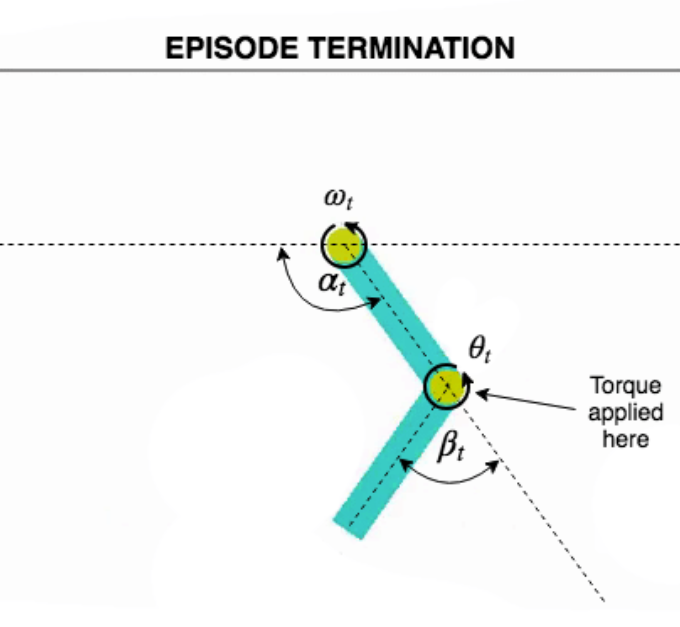
\includegraphics{thesis/images/acrobot_env.png}}}
    \caption{Trò chơi Acrobot}
    \label{fig:flappybird}
\end{figure}
Acrobot là một con lắc 2 liên kết chỉ có khớp thứ hai được kích hoạt. Ban đầu, cả hai liên kết đều hướng xuống dưới. Mục tiêu là để xoay bộ phận đầu cuối ở độ cao mà ít nhất là chiều dài của một liên kết nằm ở phía trên đường cơ sở. Cả hai liên kết có thể xoay tự do và có thể đi qua nhau, tức là, chúng không va chạm khi chúng có cùng một góc. Trò chơi bao gồm các trạng thái của môi trường là các hàm sin() và cos() của 2 khớp góc quay và vận tốc góc khớp đó là [$\cos(\theta_1)$, $\sin(\theta_1)$, $\cos(\theta_2)$, $\sin(\theta_2)$, $\Dot{\theta_1}$, $\Dot{\theta_2}$]. Đối với liên kết đầu tiên, một góc 0 tương ứng với liên kết hướng xuống dưới. Góc của liên kết thứ hai liên quan đến góc của liên kết thứ nhất. Một góc 0 tương ứng với việc có cùng một góc giữa hai liên kết. Trạng thái [1, 0, 1, 0, ..., ...] có nghĩa là cả hai liên kết đều hướng xuống dưới. Các g
hành động cung cấp là áp dụng mô-men +1, 0 hoặc -1 trên khớp nối giữa hai liên kết con lắc. 

Chiều dài của mỗi liên kết được khởi tạo ban đầu gọi là $l_1$, $l_2$, cấu hình mạng ANN được sử dụng để học là (6,8,1). Trong đồ án này sẽ định nghĩa các tác vụ dựa theo sự khác nhau về độ dài của liên kết thứ 2:
\begin{table} [H]
    \begin{center}
    \caption{Danh sách các tác vụ thực nghiệm bài toán Acrobot}
    \scalebox{0.9}{\begin{tabular}{|c|c|c|c|c|c|}
    \hline
    \multirow{1}{*}{\textbf{Tham số}} & \multicolumn{1}{c|}{\textbf{Tác vụ 1}} & \multicolumn{1}{c|}{\textbf{Tác vụ 2}} & \multicolumn{1}{c|}{\textbf{Tác vụ 3}} & \multicolumn{1}{c|}{\textbf{Tác vụ 4}} & \multicolumn{1}{c|}{\textbf{Tác vụ 5}} \\ \hline
    $l_2$ & $l_2=0.8$ & $l_2=0.9$ & $l_2=1.0$ & $l_2=1.1$ & $l_2=1.2$ \\\hline
    \end{tabular}}
    \end{center}
    \label{tab:result:flappybird}
\end{table}

\subsubsection{PixelCopter}
\begin{figure}[h!]
    \centering
    \scalebox{0.5}{\fbox{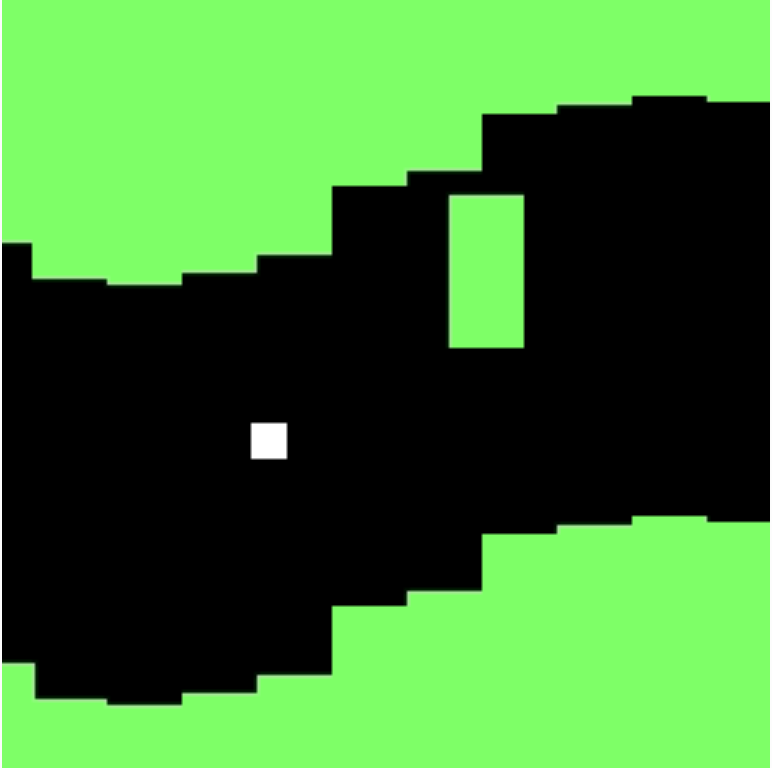
\includegraphics{thesis/images/pixelcopter.png}}}
    \caption{Trò chơi PixelCopter}
    \label{fig:flappybird}
\end{figure}
Pixelcopter là trò chơi đòi hỏi người chơi phải vượt qua các vật cản bên trong một hang động. Đây là bản sao chép của trò chơi máy bay trực thăng nổi tiếng (thuật ngữ gốc: \emph{helicopter}) với người chơi chỉ là một đơn vị pixel khiêm tốn. 
Với mỗi khối đơn vị chiều dài mà người chơi vượt qua sẽ nhận được một điểm thưởng là +1. Khi trò chơi kết thúc sẽ nhận được một điểm thưởng âm là -1. Trò chơi kết thúc khi người choi va đập vào thành hang, hoặc các chướng ngại vật trong hang. Trạng thái của trò chơi được biểu diễn bởi một véc-tơ 7 chiều mô tả vị trí của pixel và các vật cản ở gần. Để mô hình hóa policy của bài toán dưới dạng mạng ANN, đồ án sử dụng một mạng ANN có cấu trúc là (7,8,1) tương ứng với đầu vào, lớp ẩn, đầu ra của policy.

Trong môi trường của trò chơi có một tham số là momentum ảnh hưởng đến tốc độ, và vị trí sau mỗi hành động của pixel. Trong đồ án này sẽ định nghĩa các tác vụ dựa theo sự khác nhau về momentum giữa các môi trường:
\begin{table} [H]
    \begin{center}
    \caption{Danh sách các tác vụ thực nghiệm bài toán Pixelcopter}

    \scalebox{0.85}{\begin{tabular}{|c|c|c|c|c|c|}
    \hline
    \multirow{1}{*}{\textbf{Tham số}} & \multicolumn{1}{c|}{\textbf{Tác vụ 1}} & \multicolumn{1}{c|}{\textbf{Tác vụ 2}} & \multicolumn{1}{c|}{\textbf{Tác vụ 3}} & \multicolumn{1}{c|}{\textbf{Tác vụ 4}} & \multicolumn{1}{c|}{\textbf{Tác vụ 5}} \\ \hline
    momentum & $momentum=0$ & $momentum=0.1$ & $momentum=0.2$ & $momentum=0.3$ & $momentum=0.4$\\\hline
    \end{tabular}}
    \end{center}
    \label{tab:result:flappybird}
\end{table}

\subsubsection{FlappyBird}
\begin{figure}[h!]
    \centering
    \scalebox{0.5}{\fbox{
\includegraphics{flappy-bird_tbqj.jpg}}}
    \caption{Trò chơi FlappyBird}
    \label{fig:flappybird}
\end{figure}
Là trò chơi mà ở đó tác nhân (chú chim) phải vượt qua được khoảng trống giữa các ống. Trong trò chơi tác nhân chỉ thực hiện 2 hành động: hướng lên, hướng xuống. Mũi tên hướng lên khiến chim trong trò chơi sẽ đi lên, mũi trên hướng xuống khiến chim đi xuống. Trong trường hợp chim đập xuống đất, đập vào thành ống hoặc đập lên phía trên màn hình thì trò chơi sẽ kết thúc. Mỗi lượt chim qua một ống sẽ được tính là được thêm $+1$ điểm thưởng. Mỗi lần tới trạng thái kết thúc sẽ nhận được một điểm thưởng âm là $-1$. Có 8 trạng thái biểu diễn vị trí 2D của chim, vị trí của vật cản tiếp theo, vị trị của vật cản tiếp theo sau đó. Với bài toán này trong đồ án sẽ sử dụng một mạng ANN có cấu hình là $(8,4,1)$ tương ứng với đầu vào, lớp ẩn, đầu ra của mạng để có thể học được mô hình policy của bài toán.

Trong môi trường của trò chơi có một tham số là trọng lực (thuật ngữ gốc: \emph{gravity}. Trong đồ án này sẽ định nghĩa các tác vụ dựa theo sự khác nhau về trọng lực giữa các môi trường:
\begin{table} [H]
    \begin{center}
    \caption{Danh sách các tác vụ thực nghiệm bài toán FlappyBird}

    \scalebox{0.9}{\begin{tabular}{|c|c|c|c|c|c|}
    \hline
    \multirow{1}{*}{\textbf{Tham số}} & \multicolumn{1}{c|}{\textbf{Tác vụ 1}} & \multicolumn{1}{c|}{\textbf{Tác vụ 2}} & \multicolumn{1}{c|}{\textbf{Tác vụ 3}} & \multicolumn{1}{c|}{\textbf{Tác vụ 4}} & \multicolumn{1}{c|}{\textbf{Tác vụ 5}} \\ \hline
    gravity & $gravity=0.8$ & $gravity=1.8$ & $gravity=2.8$ & $gravity=3.8$ & $gravity=4.8$\\\hline
    \end{tabular}}
    \end{center}
    \label{tab:result:flappybird}
\end{table}

\section{Cài đặt thực nghiệm}
Các thực nghiệm được triển khai hoàn toàn trên hệ thống Ubuntu 18.04 LTS 64-bit với mô tả cấu hình như phía dưới:
\begin{itemize}
    \item CPU: Intel\textregistered Core\texttrademark i5-2430M CPU @ 2.40GHz × 2
    \item RAM: 6GB
    \item Ngôn ngữ lập trình: Python 3.6
    \item Mã nguồn: https://github.com/minhquang4334/mfeaii-ann-rl
\end{itemize}

\subsection{Cấu hình cho bài toán huấn luyện các mạng neural khác cấu trúc}
Các thuật toán đều chạy trên mỗi cấu hình thực nghiệm 30 lần. Độ đo hiệu quả giải thuật là MSE được thống kê trên cả bộ dữ liệu học và bộ dữ liệu kiểm định. Độ đo được thống kê trong 30 lần chạy để so sánh kết quả trung bình cùng độ lệch chuẩn.
\begin{table}[h!]
    \centering
    \caption{Cấu hình và tham số giải thuật đề xuất cho bài toán huấn luyện các mạng neural khác cấu trúc}

	\begin{tabular}{|l|c|c|c|c|}
        \hline
        \multirow{1}{*}{\textbf{Tham số}} & 
        \multicolumn{1}{c|} {\textbf{Ký hiệu}} & \multicolumn{1}{c|}{\textbf{Giá trị}}\\ \hline
        Kích thước quần thể đơn nhiệm & $N_k$ & 30\\
        Số tác vụ & $K$ & 3\\
        Kích thước quần thể đa nhiệm & $N$ & $N_k \cdot K$\\
        Số thế hệ tiến hóa & $T$ & 1000\\
        Chỉ số phân phối SBX & $\eta_c$ & 15\\
        Tỉ lệ đột biến PMU & $\sigma$ & 0.2\\
        Chỉ số đột biến PMU & $\eta_m$ & 15\\
        % pswap & - & 0.5\\
        Giá trị tham số cố định $rmp$ của thuật toán $MFEA$ & $rmp$ & 0.5\\
        Giá trị khởi tạo các phần tử trong ma trận $RMP$ & $rmp_{k,j}$ & 0\\
        Giá trị chặn dưới của từng phần tử $rmp_{kj}, k,j \in {K}$  & - & 0.1\\
        Số lần chạy thống kê & - & 30\\ \hline
    \end{tabular}
    \label{tab:config:nbit}
\end{table}
\subsection{Cấu hình cho bài toán huấn luyện nhiều mô hình học tăng cường}
Các thuật toán đều chạy trên mỗi cấu hình thực nghiệm 30 lần. Độ đo hiệu quả giải thuật là tổng phần thưởng thu được với bộ tham số hiện tại. Độ đo được thống kê trong 30 lần chạy để so sánh kết quả trung bình cùng độ lệch chuẩn.
\begin{table}[h!]
    \centering
    \caption{Cấu hình và tham số giải thuật đề xuất cho bài toán huấn luyện nhiều mô hình học tăng cường}

    \begin{tabular}{|l|c|c|c|c|}
        \hline
        \multirow{1}{*}{\textbf{Tham số}} & 
        \multicolumn{1}{c|} {\textbf{Ký hiệu}} & \multicolumn{1}{c|}{\textbf{Giá trị}}\\ \hline
        Kích thước quần thể đơn nhiệm & $N_k$ & 30\\
        Số tác vụ & $K$ & 5\\
        Kích thước quần thể đa nhiệm & $N$ & $N_k \cdot K$\\
        Số thế hệ tiến hóa & $T$ & 200\\
        Chỉ số phân phối SBX & $\eta_c$ & 15\\
        Tỉ lệ đột biến PMU & $\sigma$ & 0.2\\
        Chỉ số đột biến PMU & $\eta_m$ & 15\\
        % pswap & - & 0.5\\
        Giá trị tham số cố định $rmp$ của thuật toán $MFEA$ & $rmp$ & 0.5\\
        Giá trị khởi tạo các phần tử trong ma trận $RMP$ & $rmp_{k,j}$ & 0\\
        Giá trị chặn dưới của từng phần tử $rmp_{kj}, k,j \in {K}$  & - & 0.1\\
        Số lần chạy thống kê & - & 30\\ \hline
        
    \end{tabular}
    \label{tab:config:rl}
\end{table}


\section{Kết quả}

\subsection{Huấn luyện nhiều mô mạng neural đa lớp}
\subsubsection{Bảng kết quả thực nghiệm - mạng neural cùng độ sâu 1 lớp ẩn}

\begin{table} [H]
    \begin{center}
        \caption{Kết quả thực nghiệm bài 4-bit 1 lớp ẩn}

    \begin{tabular}{|c|c|c|c|}
    \hline
    \multirow{1}{*}{\textbf{Method}} & \multicolumn{1}{c|}{\textbf{Subtask1}} & \multicolumn{1}{c|}{\textbf{Subtask 2}} & \multicolumn{1}{c|}{\textbf{Subtask 3}} \\ \hline
    CEA & $0.0316 \pm 0.0125$ & $0.0201 \pm 0.011922$ & $0.0117 \pm 0.008133$ \\
    MFEA-I & $0.025 \pm 0.012957$ & $0.0117 \pm 0.007342$ & $0.0072 \pm 0.005355$\\
    MFEA-II  & $\mathbf{0.0219 \pm 0.009181}$ & $\mathbf{0.0099 \pm 0.007053}$ & $\mathbf{0.0052 \pm 0.004126}$ \\\hline
    
    \end{tabular}
    \end{center}
    
    \label{tab:result:nbit}
\end{table}
\begin{table} [H]   
    \begin{center}
        \caption{Kết quả thực nghiệm bài 6-bit 1 lớp ẩn}

    \begin{tabular}{|c|c|c|c|}
    \hline
    \multirow{1}{*}{\textbf{Method}} & \multicolumn{1}{c|}{\textbf{Subtask1}} & \multicolumn{1}{c|}{\textbf{Subtask 2}} & \multicolumn{1}{c|}{\textbf{Subtask 3}} \\ \hline
    CEA(5,6,7)  & $0.0703 \pm 0.014543$ & $0.0619 \pm 0.018078$ & $0.0572 \pm 0.017982$ \\
    MFEA-I(5,6,7)   & $\mathbf{0.06 \pm 0.014702}$ & $\mathbf{0.0498 \pm 0.009562}$ & $0.047 \pm 0.008464$ \\
    MFEA-II(5,6,7)  & $0.06 \pm 0.011387$ & $0.052 \pm 0.009393$ & $\mathbf{0.047 \pm 0.009579}$ \\\hline
    
    CEA(6,7,8)   & $0.0669 \pm 0.016032$ & $0.0583 \pm 0.009948$ & $0.0521 \pm 0.015598$ \\
    MFEA-I(6,7,8)  & $0.0611 \pm 0.013622$ & $0.0528 \pm 0.011122$ & $0.0484 \pm 0.011074$ \\
    MFEA-II(6,7,8) & $\mathbf{0.0522 \pm 0.011066}$ & $\mathbf{0.0476 \pm 0.01033}$ & $\mathbf{0.0418 \pm 0.011741}$ \\\hline
    
    \end{tabular}
    \end{center}
    \label{tab:result:nbit}
\end{table}    
\begin{table} [H]
    \begin{center}
        \caption{Kết quả thực nghiệm bài 8-bit 1 lớp ẩn}

    \begin{tabular}{|c|c|c|c|}
    \hline
    \multirow{1}{*}{\textbf{Method}} & \multicolumn{1}{c|}{\textbf{Subtask1}} & \multicolumn{1}{c|}{\textbf{Subtask 2}} & \multicolumn{1}{c|}{\textbf{Subtask 3}} \\ \hline
    CEA(5,6,7) & $0.0956 \pm 0.013764$ & $0.0906 \pm 0.015274$ & $0.0874 \pm 0.010884$ \\
    MFEA-I(5,6,7) & $0.0859 \pm 0.011722$ & $0.0801 \pm 0.009489$ & $0.0778 \pm 0.010507$  \\
    MFEA-II(5,6,7) & $\mathbf{0.0827 \pm 0.010678}$ & $\mathbf{0.076 \pm 0.012979}$ & $\mathbf{0.0735 \pm 0.012598}$ \\\hline
    
    CEA(6,7,8)& $0.0895 \pm 0.012499$ & $0.0902 \pm 0.013171$ & $0.081 \pm 0.013371$ \\
    MFEA-I(6,7,8)  & $0.0826 \pm 0.011089$ & $0.0768 \pm 0.010228$ & $0.0734 \pm 0.008805$ \\
    MFEA-II(6,7,8) & $\mathbf{0.0808 \pm 0.010726}$ & $\mathbf{0.0739 \pm 0.01117}$ & $\mathbf{0.072 \pm 0.009657}$ \\\hline
    \end{tabular}
    \end{center}
    \label{tab:result:nbit}
\end{table}

\subsubsection{Biểu đồ hội tụ - mạng neural cùng độ sâu 1 lớp ẩn}
\begin{figure}[H]
    \centering

    \scalebox{.7}{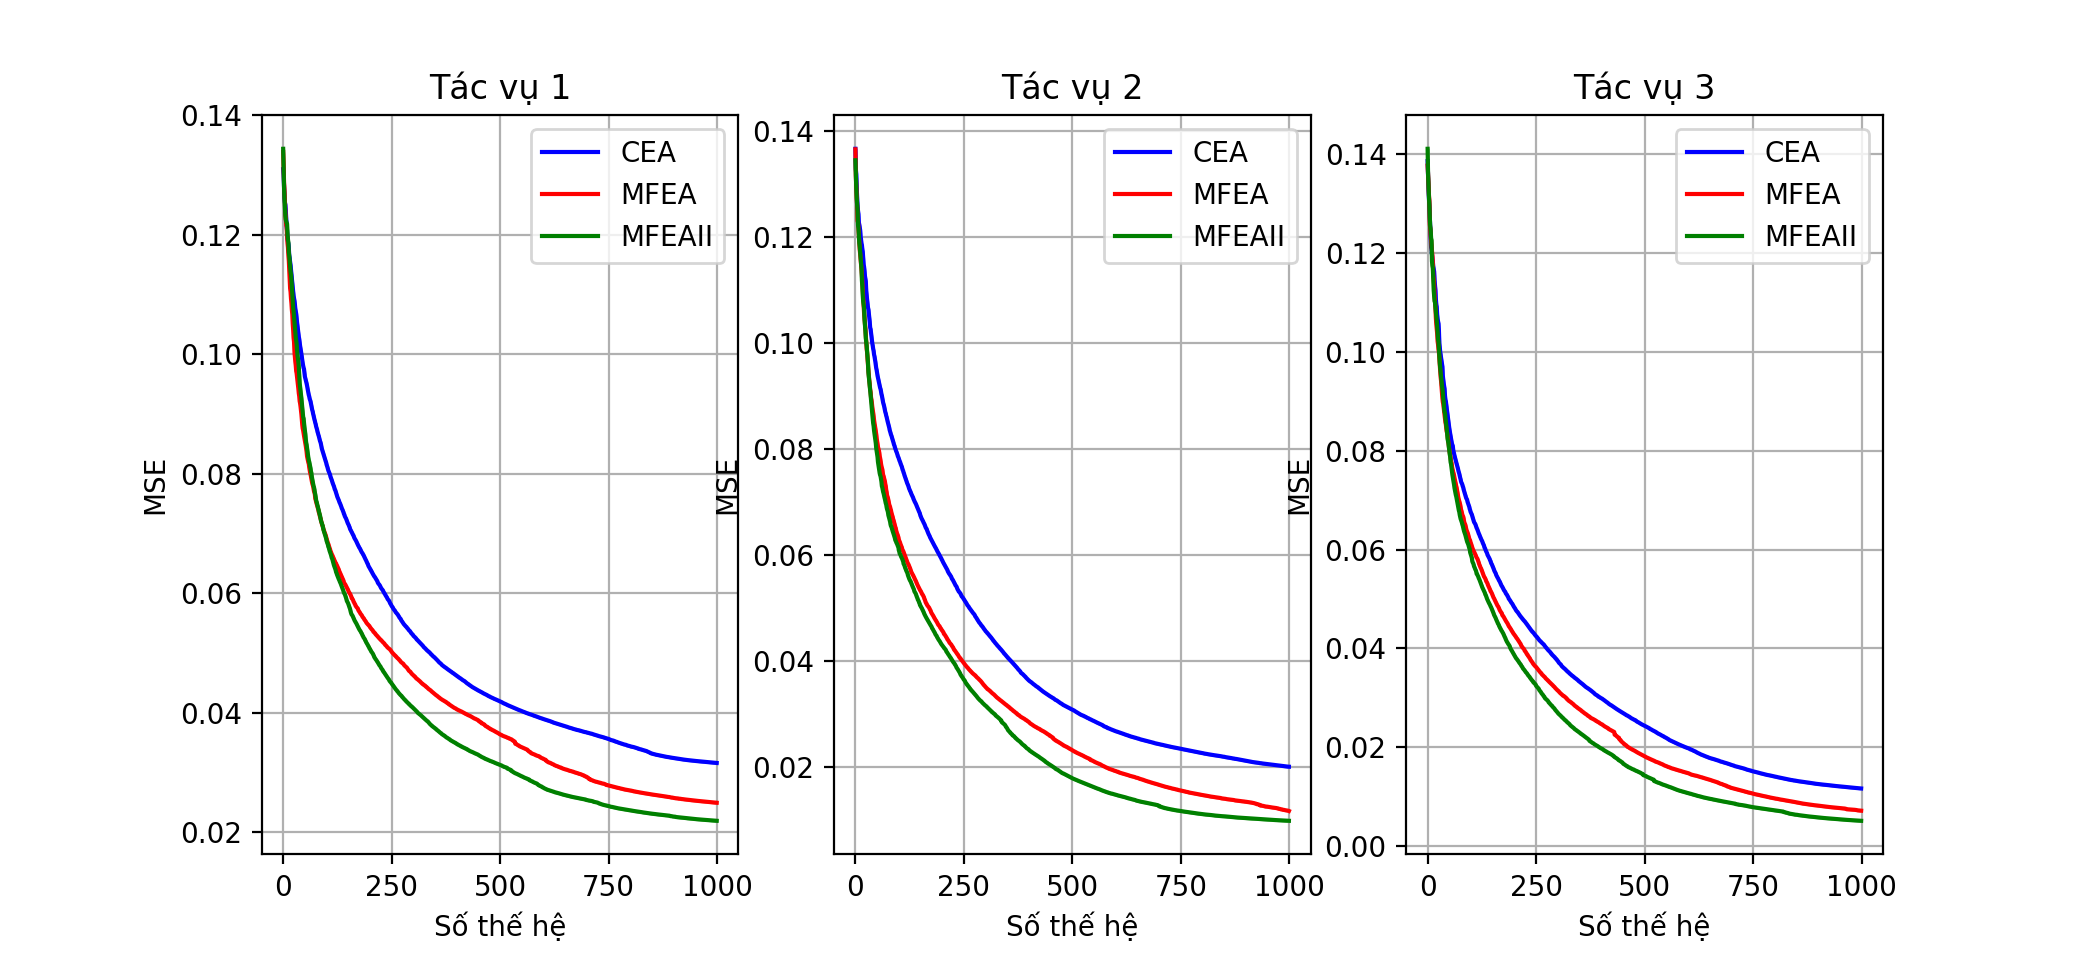
\includegraphics[width=\textwidth,height=\textheight,keepaspectratio]{thesis/images/results/nbit_1layer/4bit_task.png}}
    \scalebox{.7}{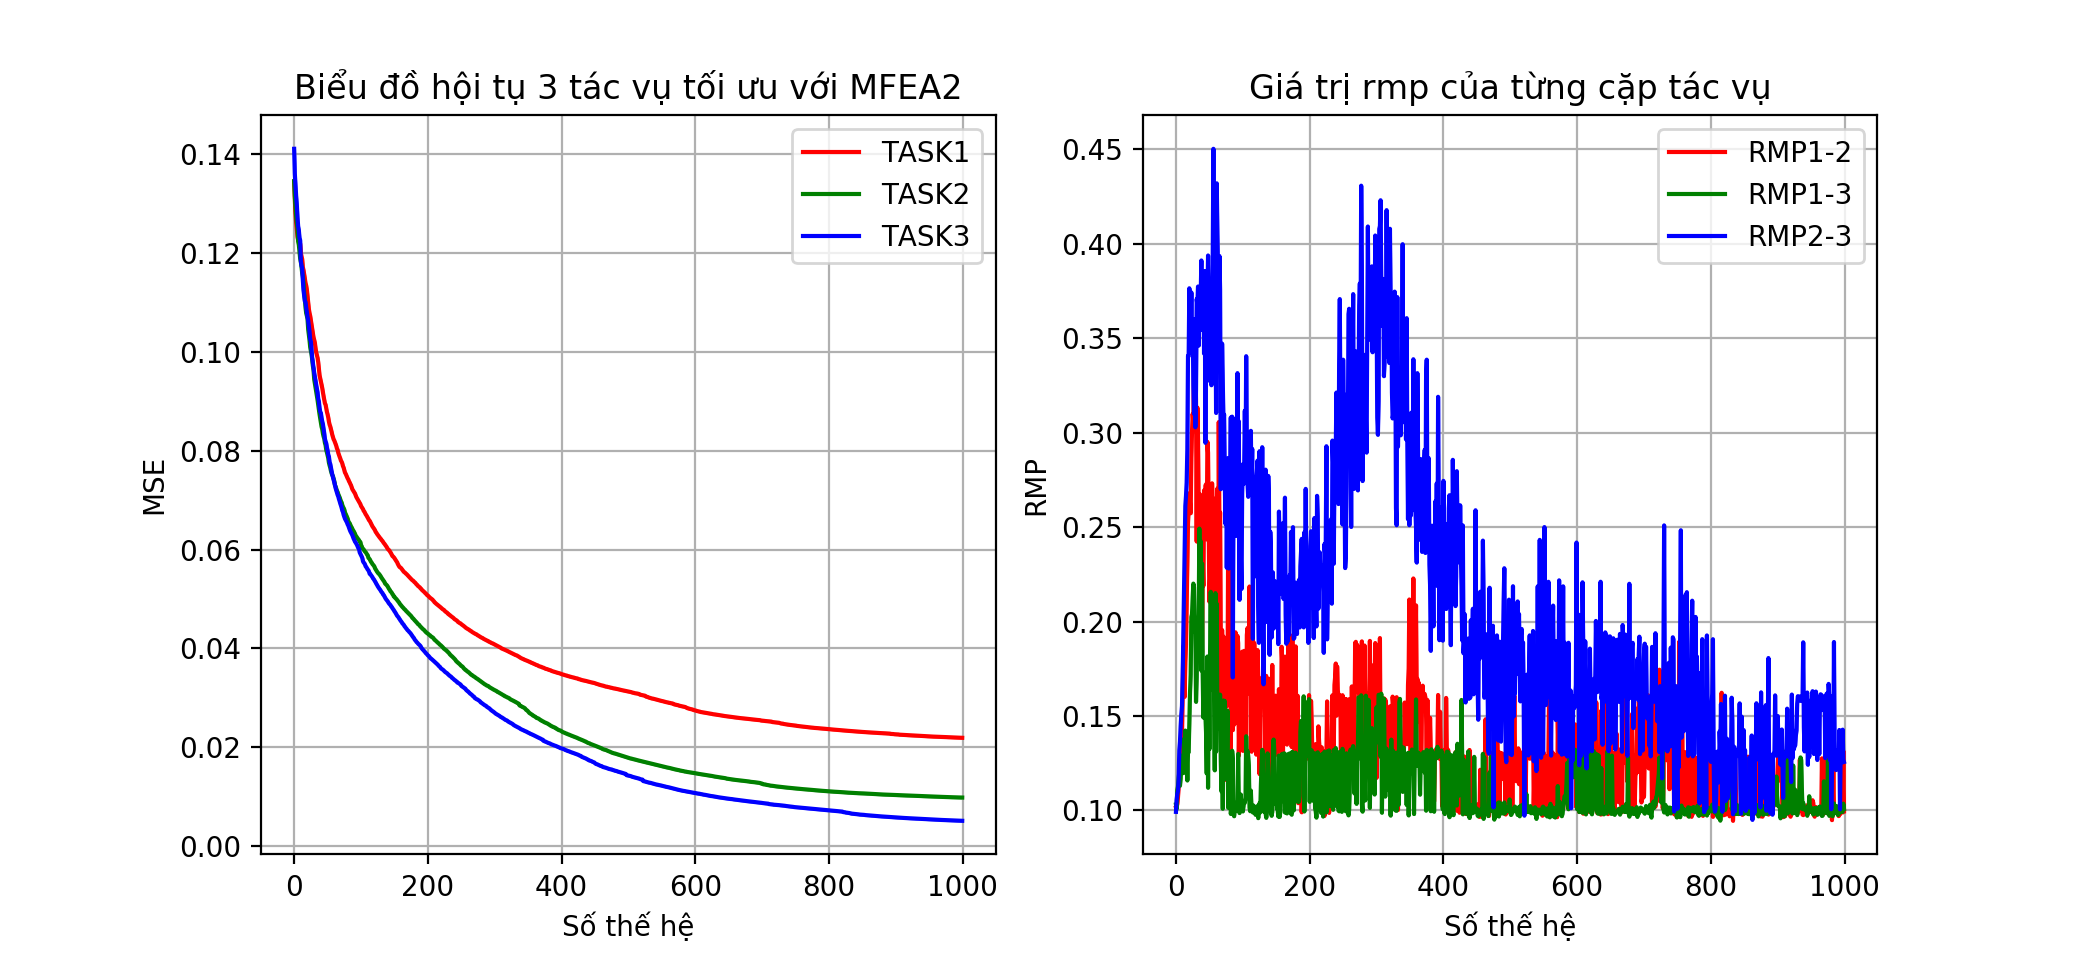
\includegraphics[width=\textwidth,height=\textheight,keepaspectratio]{thesis/images/results/nbit_1layer/4bit_rmp.png}}
    \label{fig:4bit_1layer}
    \caption{Bài 4bit: Biểu đồ hội tụ của từng tác vụ trên các thuật toán và biểu đồ phân tích MFEA-II theo giá trị rmp}

\end{figure}
\begin{figure}[H]
    \centering
    \scalebox{.7}{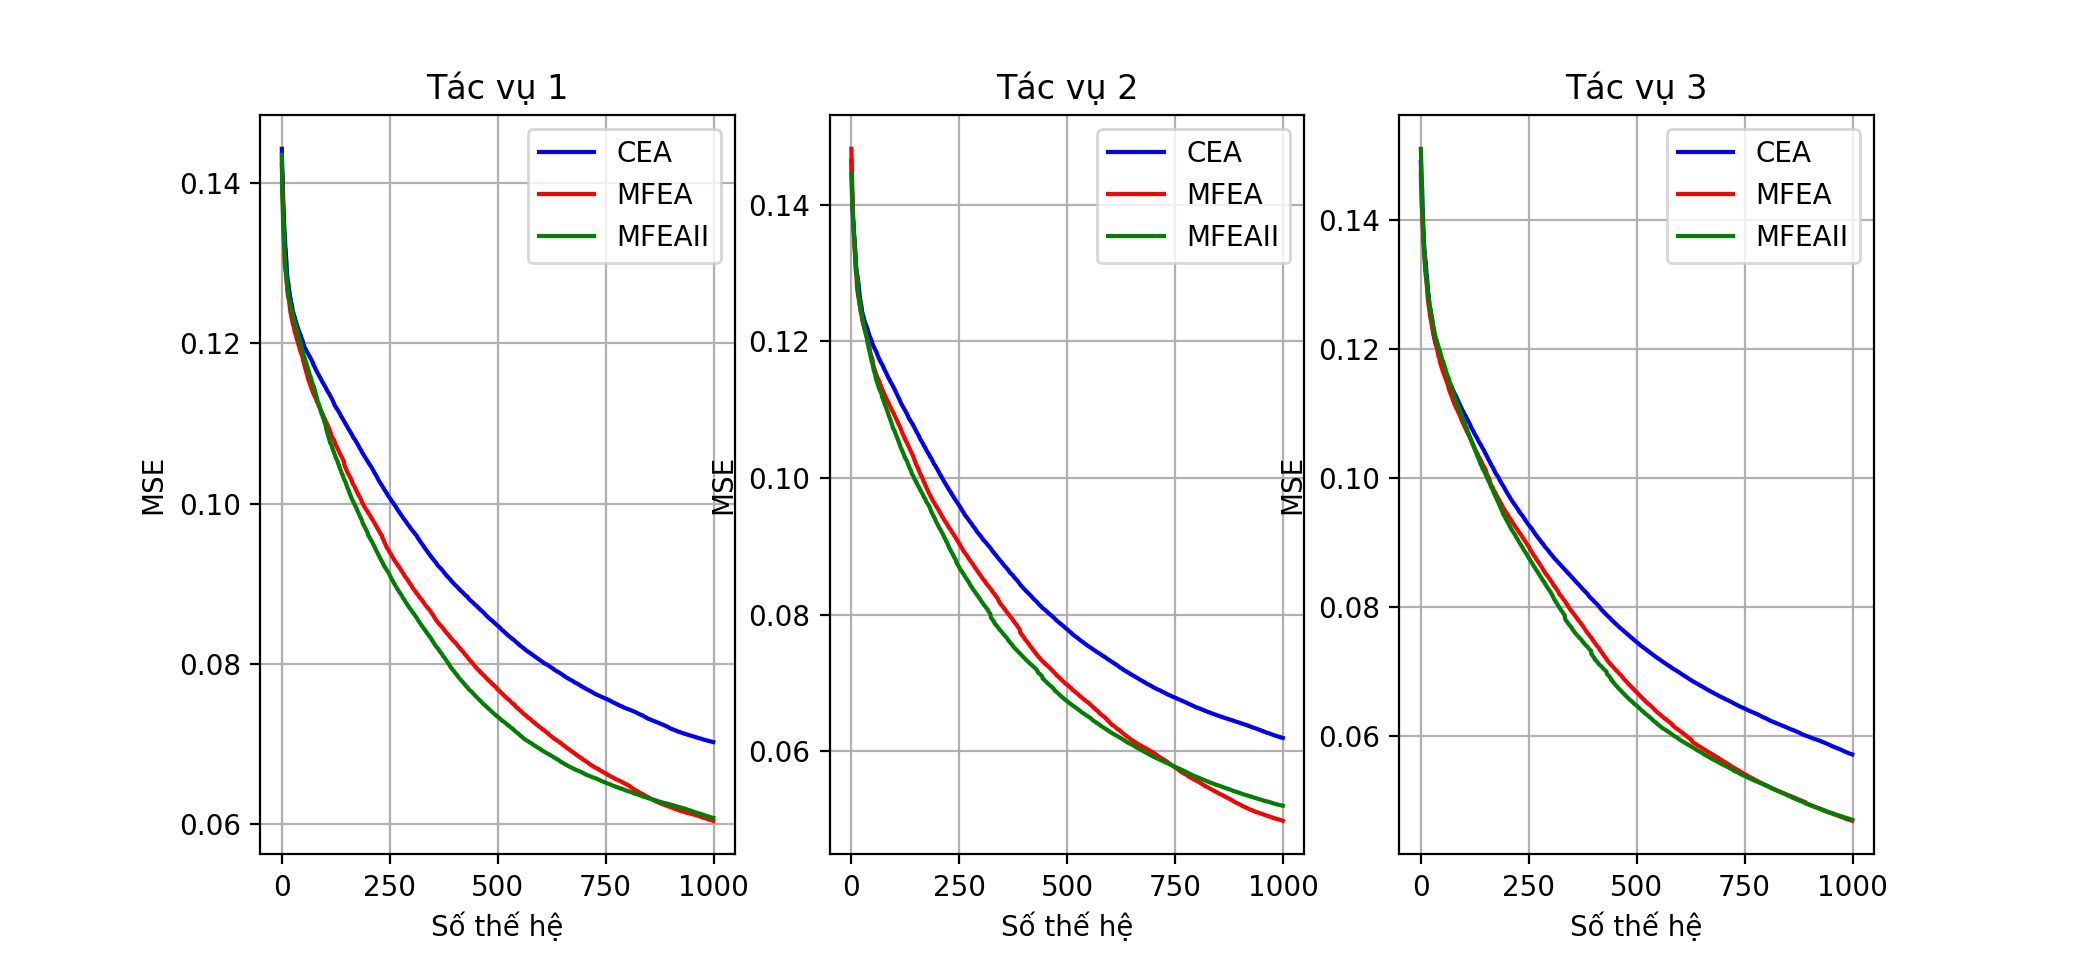
\includegraphics[width=\textwidth,height=\textheight,keepaspectratio]{thesis/images/results/nbit_1layer/6bit1_task.png}}
    \scalebox{.7}{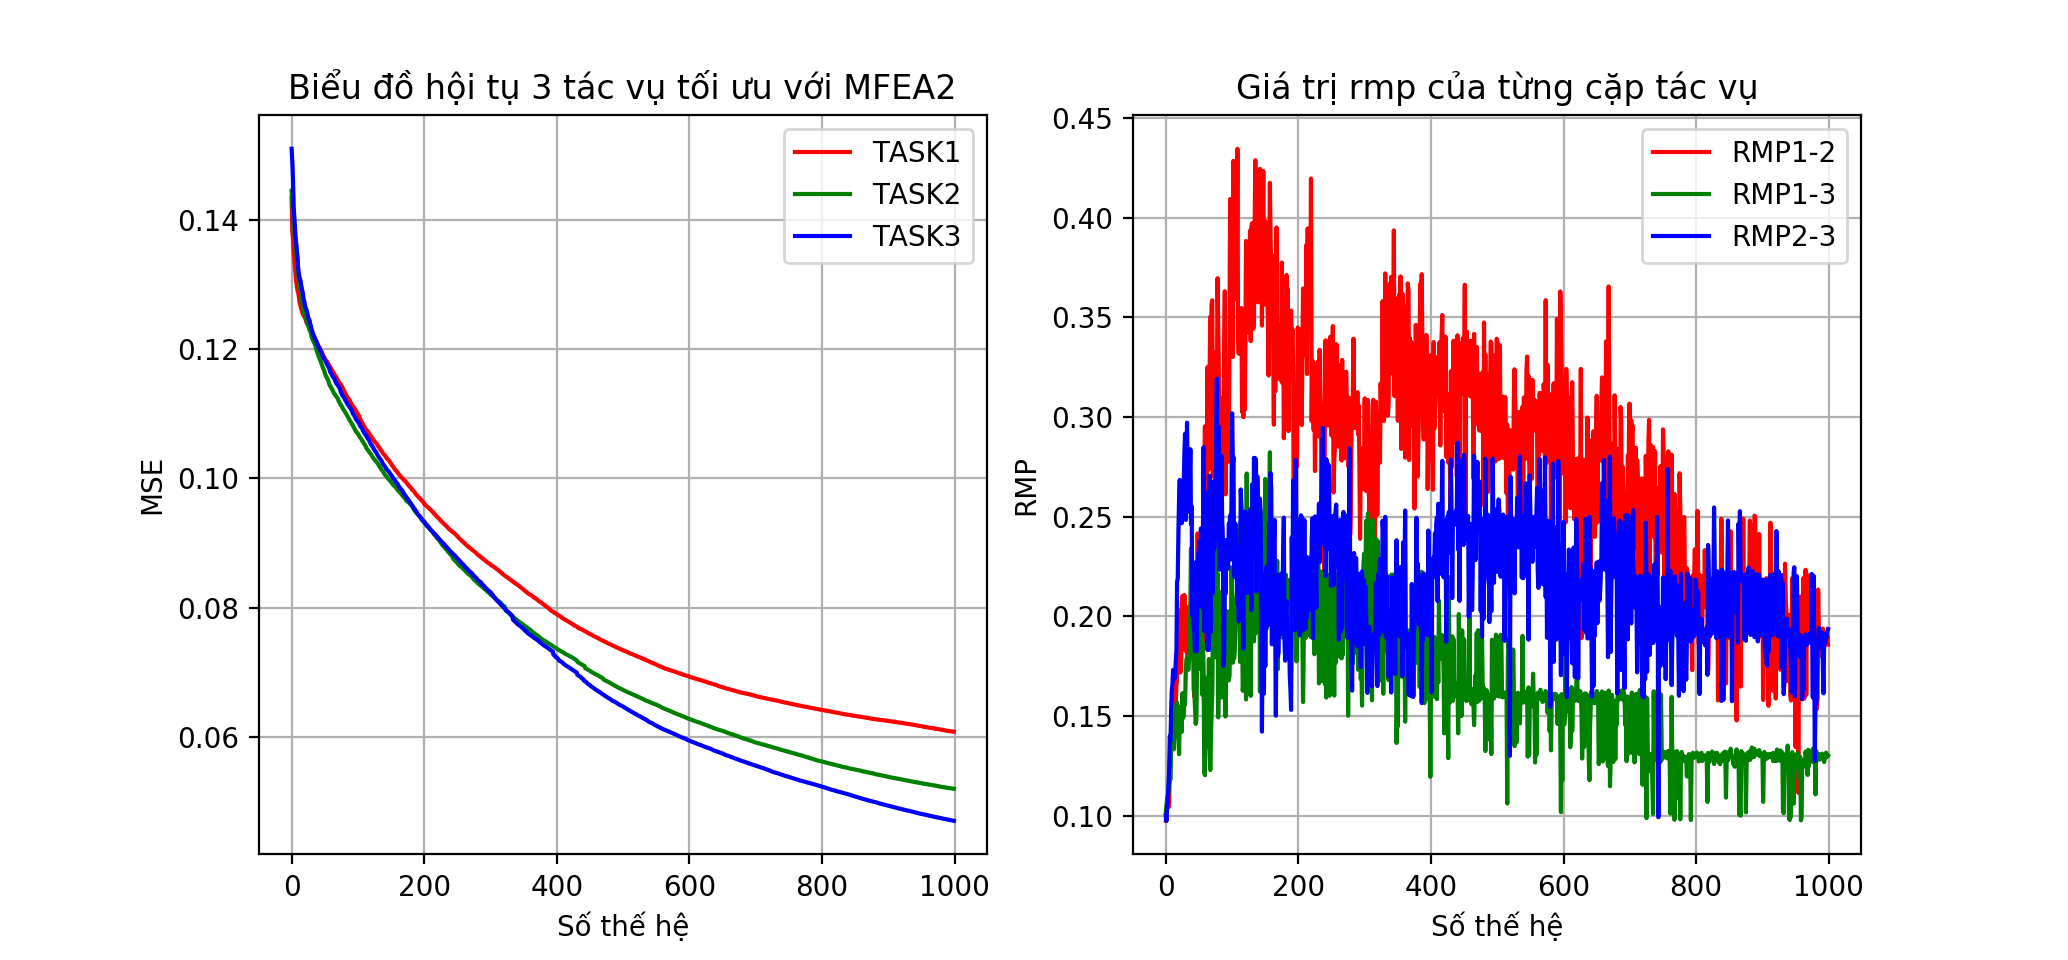
\includegraphics[width=\textwidth,height=\textheight,keepaspectratio]{thesis/images/results/nbit_1layer/6bit1_rmp.png}}
    \label{fig:6bit_1}
    \caption{Bài 6bit(5,6,7): Biểu đồ hội tụ của từng tác vụ trên các thuật toán và biểu đồ phân tích MFEA-II theo giá trị rmp}

\end{figure}
\begin{figure}[H]

    \centering
    \scalebox{.7}{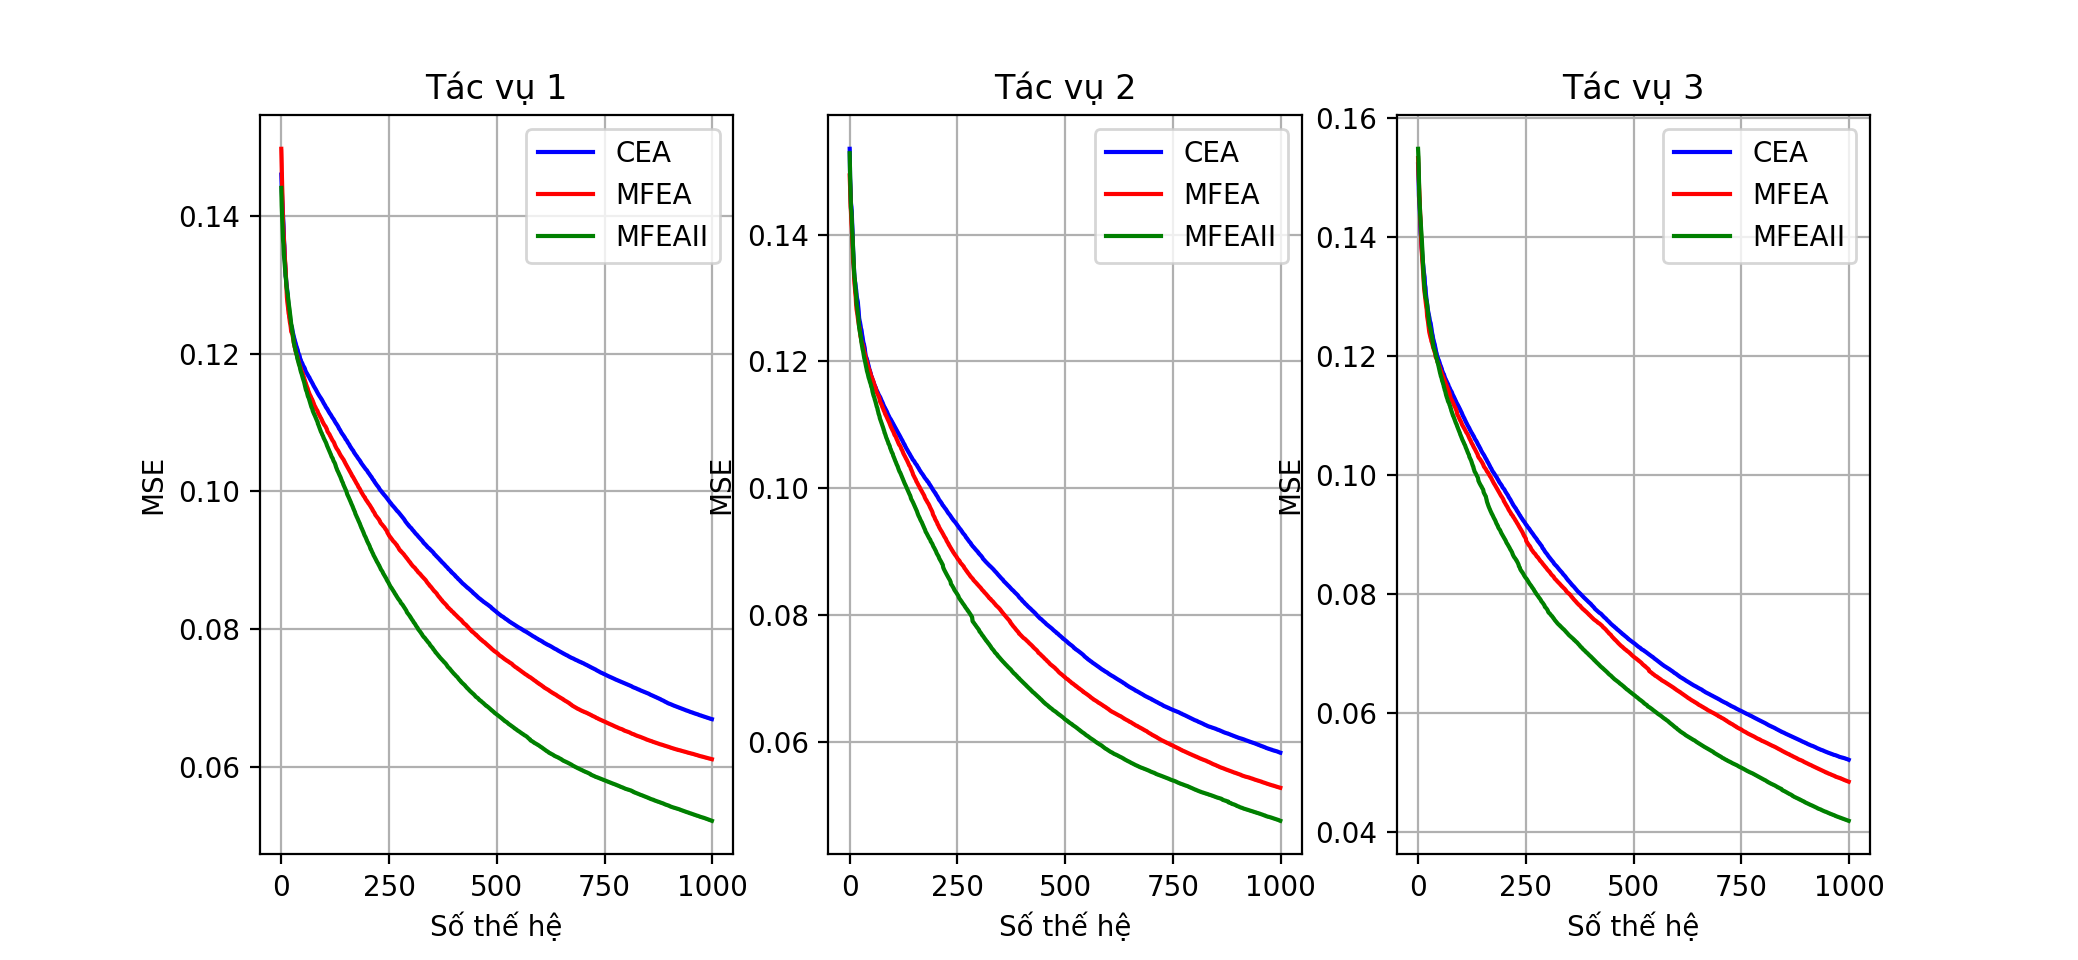
\includegraphics[width=\textwidth,height=\textheight,keepaspectratio]{thesis/images/results/nbit_1layer/6bit2_task.png}}
    \scalebox{.7}{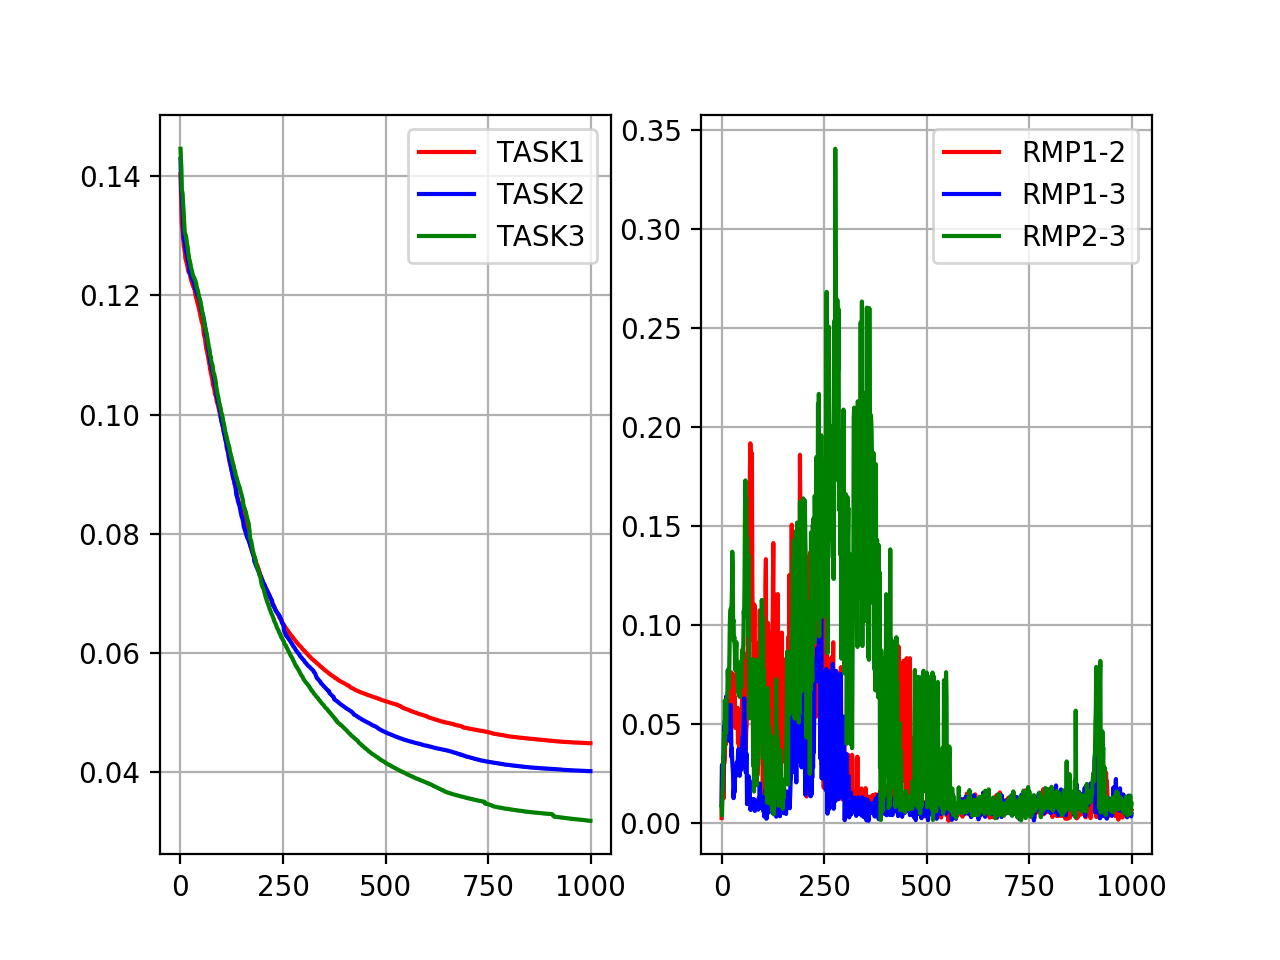
\includegraphics[width=\textwidth,height=\textheight,keepaspectratio]{thesis/images/results/nbit_1layer/6bit2_rmp.png}}
    \label{fig:6bit2_1layer}
        \caption{Bài 6bit(6,7,8): Biểu đồ hội tụ của từng tác vụ trên các thuật toán và biểu đồ phân tích MFEA-II theo giá trị rmp}

\end{figure}
\begin{figure}[H]
    \centering

    \scalebox{.7}{\includegraphics[width=\textwidth,height=\textheight,keepaspectratio]{thesis/images/results/nbit_1layer/8bit1_task.png}}
    \scalebox{.7}{\includegraphics[width=\textwidth,height=\textheight,keepaspectratio]{thesis/images/results/nbit_1layer/8bit1_rmp.png}}
    \label{fig:8bit1_1layer}
    \caption{Bài 8bit(5,6,7):Biểu đồ hội tụ của từng tác vụ trên các thuật toán và biểu đồ phân tích MFEA-II theo giá trị rmp}

\end{figure}
\begin{figure}[H]
    \centering

    \scalebox{.7}{\includegraphics[width=\textwidth,height=\textheight,keepaspectratio]{thesis/images/results/nbit_1layer/8bit2_task.png}}
    \scalebox{.7}{\includegraphics[width=\textwidth,height=\textheight,keepaspectratio]{thesis/images/results/nbit_1layer/8bit2_rmp.png}}
    \label{fig:8bit2_1layer}
    \caption{Bài 8bit(6,7,8): Biểu đồ hội tụ của từng tác vụ trên các thuật toán và biểu đồ phân tích MFEA-II theo giá trị rmp}

\end{figure}

\subsubsection{Bảng kết quả thực nghiệm - mạng neural cùng độ sâu 2 lớp ẩn}
\begin{table} [H]
    \begin{center}
    \caption{Kết quả thực nghiệm huấn luyện ANN 2 lớp ẩn}
    \begin{tabular}{|c|c|c|c|c|}
    \hline
    \multirow{1}{*}{\textbf{Bài toán}} &
    \multirow{1}{*}{\textbf{Method}} & \multicolumn{1}{c|}{\textbf{Tác vụ 1}} & \multicolumn{1}{c|}{\textbf{Tác vụ 2}} & \multicolumn{1}{c|}{\textbf{Tác vụ 3}} \\ \hline
    \multirow{3}{*} 
    {8-bit} &
    CEA & $0.075 \pm 0.012865$ & $0.0713 \pm 0.013116$ & $0.0718 \pm 0.012432$  \\
    & MFEA-I & $0.0738 \pm 0.012508$ & $0.0684 \pm 0.013252$ & $0.0669 \pm 0.015076$   \\
    & MFEA-II & $\mathbf{0.0705 \pm 0.012856}$ & $\mathbf{0.0624 \pm 0.011079}$ & $\mathbf{0.0595 \pm 0.011252}$\\\hline
    \multirow{3}{*} 
    {9-bit} &
    CEA & $0.0826 \pm 0.010588$ & $0.0751 \pm 0.014406$ & $0.0785 \pm 0.010766$  \\
    & MFEA-I & $0.0827 \pm 0.010438$ & $0.0762 \pm 0.009495$ & $0.0737 \pm 0.009766$ \\
    & MFEA-II & $\mathbf{0.0795 \pm 0.012865}$ & $\mathbf{0.0705 \pm 0.009581}$ & $\mathbf{0.0685 \pm 0.011156}$ \\\hline
    \multirow{3}{*} 
    {10-bit} &
    CEA & $0.0853 \pm 0.01105$ & $0.0862 \pm 0.008326$ & $0.0856 \pm 0.008919$  \\
    & MFEA-I  & $0.0855 \pm 0.012229$ & $\mathbf{0.0782 \pm 0.009659}$ & $\mathbf{0.0752 \pm 0.009681}$ \\
    & MFEA-II & $\mathbf{0.0833 \pm 0.010222}$ & $0.0791 \pm 0.009846$ & $0.0762 \pm 0.010419$ \\\hline
    \end{tabular}
    \end{center}

    \label{tab:result:nbit}
\end{table}

\subsubsection{Biểu đồ hội tụ - Mạng neural cùng độ sâu 2 lớp ẩn}
\begin{figure}[h!]
    \centering
    \scalebox{.7}{\includegraphics[width=\textwidth,height=\textheight,keepaspectratio]{thesis/images/results/nbit_2layer/8bit1_task.png}}
    \scalebox{.7}{\includegraphics[width=\textwidth,height=\textheight,keepaspectratio]{thesis/images/results/nbit_2layer/8bit1_rmp.png}}
    \caption{Bài 8bit: Biểu đồ hội tụ của từng tác vụ trên các thuật toán và biểu đồ phân tích MFEA-II theo giá trị rmp}
    \label{fig:8bit_2layer}
\end{figure}
\begin{figure}[h!]
    \centering
    \scalebox{.7}{\includegraphics[width=\textwidth,height=\textheight,keepaspectratio]{thesis/images/results/nbit_2layer/9bit1_task.png}}
    \scalebox{.7}{\includegraphics[width=\textwidth,height=\textheight,keepaspectratio]{thesis/images/results/nbit_2layer/9bit1_rmp.png}}
    \caption{Bài 9bit: Biểu đồ hội tụ của từng tác vụ trên các thuật toán và biểu đồ phân tích MFEA-II theo giá trị rmp}
    \label{fig:9bit_2layer}
\end{figure}
\begin{figure}[h!]
    \centering
    \scalebox{.7}{\includegraphics[width=\textwidth,height=\textheight,keepaspectratio]{thesis/images/results/nbit_2layer/10bit1_task.png}}
    \scalebox{.7}{\includegraphics[width=\textwidth,height=\textheight,keepaspectratio]{thesis/images/results/nbit_2layer/10bit1_rmp.png}}
    \caption{Bài 10bit: Biểu đồ hội tụ của từng tác vụ trên các thuật toán và biểu đồ phân tích MFEA-II theo giá trị rmp}
    \label{fig:10bit_2layer}
\end{figure}
\newpage

\subsubsection{Bảng kết quả thực nghiệm - mạng neural khác độ sâu}
\begin{table} [H]
    \begin{center}
    \caption{Kết quả huấn luyện ANN khác độ sâu}
    \begin{tabular}{|c|c|c|c|c|}
    \hline
    \multirow{1}{*}{\textbf{Bài toán}} &
    \multirow{1}{*}{\textbf{Method}} & \multicolumn{1}{c|}{\textbf{Tác vụ 1}} & \multicolumn{1}{c|}{\textbf{Tác vụ 2}} & \multicolumn{1}{c|}{\textbf{Tác vụ 3}} \\ \hline
    \multirow{3}{*} 
    {8-bit} &
    CEA & $0.0789 \pm 0.0172$ & $0.0815 \pm 0.0136$ & $\mathbf{0.0794 \pm 0.0156}$ \\
    & MFEA-I & $0.0778 \pm 0.0153$ & $0.0805 \pm 0.0142$ & $0.0814 \pm 0.0119$  \\
    & MFEA-II & $\mathbf{0.0721} \pm 0.0148$ & $\mathbf{0.0759 \pm 0.015}$ & $0.0822 \pm 0.0143$\\\hline
    \multirow{3}{*} 
    {9-bit} &
    CEA & $0.0843 \pm 0.0154$ & $0.0869 \pm 0.0141$ & $0.086 \pm 0.0128$  \\
    & MFEA-I & $0.0844 \pm 0.0124$ & $\mathbf{0.0795 \pm 0.0144}$ & $\mathbf{0.081 \pm 0.0134}$ \\
    & MFEA-II & $\mathbf{0.0828 \pm 0.0129}$ & $0.0818 \pm 0.0131$ & $0.0864 \pm 0.0147$ \\\hline
    \multirow{3}{*} 
    {10-bit} &
    CEA & $0.089 \pm 0.0131$ & $0.0922 \pm 0.0164$ & $0.0928 \pm 0.0124$  \\
    & MFEA-I  & $0.0879 \pm 0.0091$ & $0.0888 \pm 0.0124$ & $\mathbf{0.0873 \pm 0.0111}$ \\
    & MFEA-II & $\mathbf{0.0867 \pm 0.0079}$ & $\mathbf{0.0862 \pm 0.0103}$ & $0.0905 \pm 0.0104$ \\\hline
    \end{tabular}
    \end{center}
    \label{tab:result:nbit}

\end{table}

\subsubsection{Biểu đồ hội tụ - mạng neural khác độ sâu}

\begin{figure}[h!]
    \centering
    \scalebox{.57}{\includegraphics[width=\textwidth,height=\textheight,keepaspectratio]{thesis/images/results/multilayers/8bit2_task.png}}
    \scalebox{.57}{\includegraphics[width=\textwidth,height=\textheight,keepaspectratio]{thesis/images/results/multilayers/8bit2_rmp.png}}
    \caption{Bài 8bit: Biểu đồ hội tụ của từng tác vụ trên các thuật toán và biểu đồ phân tích MFEA-II theo giá trị rmp}
    \label{fig:8bit_multilayer}
\end{figure}
\begin{figure}[h!]
    \centering
    \scalebox{.6}{\includegraphics[width=\textwidth,height=\textheight,keepaspectratio]{thesis/images/results/multilayers/9bit2_task.png}}
    \scalebox{.6}{\includegraphics[width=\textwidth,height=\textheight,keepaspectratio]{thesis/images/results/multilayers/9bit2_rmp.png}}
    \caption{Bài 9bit: Biểu đồ hội tụ của từng tác vụ trên các thuật toán và biểu đồ phân tích MFEA-II theo giá trị rmp}
    \label{fig:8bit_multilayer}
\end{figure}
\begin{figure}[h!]
    \centering
    \scalebox{.5}{\includegraphics[width=\textwidth,height=\textheight,keepaspectratio]{thesis/images/results/multilayers/10bit2_task.png}}
    \scalebox{.5}{\includegraphics[width=\textwidth,height=\textheight,keepaspectratio]{thesis/images/results/multilayers/10bit2_rmp.png}}
    \caption{Bài 10bit: Biểu đồ hội tụ của từng tác vụ trên các thuật toán và biểu đồ phân tích MFEA-II theo giá trị rmp}
    \label{fig:8bit_multilayer}
\end{figure}

\subsubsection{Bảng kết quả thực nghiệm - bộ dữ liệu UCI với mạng neural cùng độ sâu}
\begin{table}[h!]
    \caption{Kết quả huấn luyện nhiều ANN trên bộ dữ liệu UCI cùng độ sâu}

    \begin{tabular}{|c|c|c|c|c|}
    \hline
    \multirow{1}{*}{\textbf{Instance}} & \multicolumn{1}{c|} {\textbf{Method}} & \multicolumn{1}{c|}{\textbf{Subtask1}} & \multicolumn{1}{c|}{\textbf{Subtask 2}} & \multicolumn{1}{c|}{\textbf{Subtask 3}} \\ \hline
    \multirow{3}{*} 
    {breastCancer} & CEA & $0.0097 \pm 0.0012$ & $0.0092 \pm 0.0007$ & $0.0093 \pm 0.0009$ \\
     & MFEA-I & $0.0097 \pm 0.0006$ & $0.0093 \pm 0.0005$ & $0.0091 \pm 0.0005$ \\ 
    & MFEA II & $\mathbf{0.0094 \pm 0.0008}$ & $\mathbf{0.0089 \pm 0.0006}$ & $\mathbf{0.0087 \pm 0.0004}$ \\ \hline
    \multirow{3}{*} {creditScreening} & CEA & $0.0509 \pm 0.0033$ & $0.0514 \pm 0.0033$ & $0.0508 \pm 0.004$ \\
   & MFEA-I & $0.0504 \pm 0.0024$ & $0.0503 \pm 0.0025$ & $0.0513 \pm 0.0022$ \\ 
   & MFEA-II & $\mathbf{0.0492 \pm 0.0023}$ & $\mathbf{0.0489 \pm 0.002}$ & $\mathbf{0.0491 \pm 0.002}$ \\ \hline
    \multirow{3}{*} {ionosphere} & CEA & $0.0384 \pm 0.0072$ & $0.0389 \pm 0.0129$ & $0.035 \pm 0.0047$ \\
    &MFEA-I & $0.0367 \pm 0.0068$ & $0.0347 \pm 0.0075$ & $0.0351 \pm 0.0088$ \\
    &MFEA-II & $\mathbf{0.0343 \pm 0.0079}$ & $\mathbf{0.0322 \pm 0.0071}$ & $\mathbf{0.032 \pm 0.007}$ \\\hline
    \multirow{3}{*} {ticTacToe} & CEA & $0.089 \pm 0.0047$ & $0.0838 \pm 0.0054$ & $0.0869 \pm 0.0049$ \\
    &MFEA-I & $0.0845 \pm 0.0049$ & $0.0818 \pm 0.0047$ & $0.0824 \pm 0.0047$ \\
    &MFEA-II & $\mathbf{0.082 \pm 0.0048}$ & $\mathbf{0.0815 \pm 0.0046}$ & $\mathbf{0.0812 \pm 0.0043}$  \\\hline
    
    \end{tabular}

    \label{tab:result:nbit}
\end{table}
\subsubsection{Biểu đồ hội tụ - bộ dữ liệu UCI với mạng neural cùng độ sâu}

\begin{figure}[h!]
    \centering
    \scalebox{.7}{\includegraphics[width=\textwidth,height=\textheight,keepaspectratio]{thesis/images/results/uci/br1_task.png}}
    \scalebox{.7}{\includegraphics[width=\textwidth,height=\textheight,keepaspectratio]{thesis/images/results/uci/br1_rmp.png}}
    \caption{Biểu đồ hội tụ của các tác vụ bài BreastCancer cùng độ sâu}
    \label{fig:br_mtl}
\end{figure}

\begin{figure}[h!]
    \centering
    \scalebox{.7}{\includegraphics[width=\textwidth,height=\textheight,keepaspectratio]{thesis/images/results/uci/is1_task.png}}
    \scalebox{.7}{\includegraphics[width=\textwidth,height=\textheight,keepaspectratio]{thesis/images/results/uci/is1_rmp.png}}
    \caption{Biểu đồ hội tụ của các tác vụ bài Ionosphere cùng độ sâu}
    \label{fig:br_mtl}
\end{figure}
\newpage
\subsubsection{Bảng kết quả thực nghiệm - bộ dữ liệu UCI với mạng neural khác độ sâu}
% \begin{table}[h!]
%     \caption{Huấn luyện nhiều ANN trên bộ dữ liệu UCI khác độ sâu}
%     \begin{tabular}{|c|c|c|c|c|}
%     \hline
%     \multirow{1}{*}{\textbf{Instance}} & \multicolumn{1}{c|} {\textbf{Method}} & \multicolumn{1}{c|}{\textbf{Subtask1}} & \multicolumn{1}{c|}{\textbf{Subtask 2}} & \multicolumn{1}{c|}{\textbf{Subtask 3}} \\ \hline
%     \multirow{3}{*} 
%     {breastCancer} & CEA & $0.0119 \pm 0.0029$ & $0.0107 \pm 0.002$ & $\mathbf{0.0093 \pm 0.0005}$ \\
%      & MFEA-I & $\mathbf{0.011 \pm 0.0015}$ & $0.0102 \pm 0.0012$ & $0.0094 \pm 0.0005$  \\ 
%     & MFEA II & $\mathbf{0.011 \pm 0.0015}$ & $\mathbf{0.01 \pm 0.0011}$ & $0.0096 \pm 0.0011$ \\ \hline
    
%     \multirow{3}{*} {creditScreening} & CEA & $0.054 \pm 0.0071$ & $0.0503 \pm 0.0027$ & $0.0485 \pm 0.0017$ \\
%   & MFEA-I & $\mathbf{0.0508 \pm 0.0023}$ & $0.0497 \pm 0.0019$ & $0.0496 \pm 0.0021$ \\ 
%   & MFEA-II & $0.0515 \pm 0.0033$ & $\mathbf{0.0494 \pm 0.0023}$ & $\mathbf{0.0485 \pm 0.0018}$ \\ \hline
   
%     \multirow{3}{*} {ionosphere} & CEA & $0.0516 \pm 0.0124$ & $0.0449 \pm 0.0114$ & $0.0366 \pm 0.0094$ \\
%     &MFEA-I & $0.049 \pm 0.0131$ & $0.0413 \pm 0.0112$ & $\mathbf{0.0365 \pm 0.007}$ \\
%     &MFEA-II & $\mathbf{0.0473 \pm 0.0083}$ & $\mathbf{0.0387 \pm 0.0109}$ & $0.0367 \pm 0.008$  \\\hline
    
%     \multirow{3}{*} {ticTacToe} & CEA & $0.0899 \pm 0.0067$ & $0.0879 \pm 0.0079$ & $0.0852 \pm 0.0045$  \\
%     &MFEA-I & $\mathbf{0.088 \pm 0.008}$ & $0.0886 \pm 0.0064$ & $0.0843 \pm 0.0092$  \\
%     &MFEA-II & $\mathbf{0.088 \pm 0.0073}$ & $\mathbf{0.0832 \pm 0.0067}$ & $0\mathbf{.0817 \pm 0.0046}$  \\\hline
    
%     \end{tabular}

%     \label{tab:result:nbit}
% \end{table}
\begin{table}[h!]
    \caption{Kết quả huấn luyện nhiều ANN trên bộ dữ liệu UCI khác độ sâu}
    \begin{tabular}{|c|c|c|c|c|}
    \hline
    \multirow{1}{*}{\textbf{Instance}} & \multicolumn{1}{c|} {\textbf{Method}} & \multicolumn{1}{c|}{\textbf{Subtask1}} & \multicolumn{1}{c|}{\textbf{Subtask 2}} & \multicolumn{1}{c|}{\textbf{Subtask 3}} \\ \hline
    \multirow{3}{*} 
    {breastCancer} & CEA & $0.0082 \pm 0.0006$ & $0.0083 \pm 0.0006$ & $0.008 \pm 0.0004$ \\
     & MFEA-I & $0.0084 \pm 0.0007$ & $0.0081 \pm 0.0006$ & $0.008 \pm 0.0004$  \\ 
    & MFEA II & $\mathbf{0.0082 \pm 0.0006}$ & $\mathbf{0.008 \pm 0.0004}$ & $\mathbf{0.008 \pm 0.0004}$ \\ \hline
    
    \multirow{3}{*} {creditScreening} & CEA & $0.0442 \pm 0.0016$ & $0.0436 \pm 0.0011$ & $0.0435 \pm 0.0011$ \\
   & MFEA-I & $0.0446 \pm 0.0017$ & $\mathbf{0.0435 \pm 0.0012}$ & $0.0438 \pm 0.0013$ \\ 
   & MFEA-II & $\mathbf{0.0442 \pm 0.0016}$ & $0.0437 \pm 0.0014$ & $\mathbf{0.0433 \pm 0.0012}$ \\ \hline
   
    \multirow{3}{*} {ionosphere} & CEA & $\mathbf{0.0223 \pm 0.0064}$ & $\mathbf{0.0189 \pm 0.005}$ & $\mathbf{0.018 \pm 0.0063}$ \\
    &MFEA-I & $0.0257 \pm 0.01$ & $0.0213 \pm 0.0082$ & $0.0201 \pm 0.0076$ \\
    &MFEA-II & $0.0243 \pm 0.0055$ & $0.0199 \pm 0.0055$ & $0.0203 \pm 0.0062$  \\\hline
    
    \multirow{3}{*} {ticTacToe} & CEA & $0.0747 \pm 0.0077$ & $0.0728 \pm 0.0093$ & $0.0731 \pm 0.0061$   \\
    &MFEA-I & $0.0736 \pm 0.0103$ & $0.0724 \pm 0.008$ & $0.0704 \pm 0.0067$   \\
    &MFEA-II & $\mathbf{0.0709 \pm 0.0096}$ & $\mathbf{0.0667 \pm 0.0066}$ & $\mathbf{0.0684 \pm 0.0067}$  \\\hline
    
    \end{tabular}

    \label{tab:result:nbit}
\end{table}

\newpage
\subsubsection{Biểu đồ hội tụ - bộ dữ liệu UCI với mạng neural cùng độ sâu}

\begin{figure}[h!]
    \centering
    \scalebox{.7}{\includegraphics[width=\textwidth,height=\textheight,keepaspectratio]{thesis/images/results/uci/br_task.png}}
    \scalebox{.7}{\includegraphics[width=\textwidth,height=\textheight,keepaspectratio]{thesis/images/results/uci/br_rmp.png}}
    \caption{Biểu đồ hội tụ bài BreastCancer khác độ sâu}
    \label{fig:br_mtl}
\end{figure}

\begin{figure}[h!]
    \centering
    \scalebox{.7}{\includegraphics[width=\textwidth,height=\textheight,keepaspectratio]{thesis/images/results/uci/tt_task.png}}
    \scalebox{.7}{\includegraphics[width=\textwidth,height=\textheight,keepaspectratio]{thesis/images/results/uci/tt_rmp.png}}
    \caption{Biểu đồ hội tụ bài Tictactoe khác độ sâu}
    \label{fig:br_mtl}
\end{figure}
\pagebreak

\subsection{Kết quả huấn luyện trên các môi trường học tăng cường}
% \begin{table}
%     \caption{Mô hình học tăng cường khác môi trường}
%     \begin{center}
%     \begin{tabular}{|c|c|c|c|c|c|}
%     \hline
%     \multirow{1}{*}{\textbf{Trọng lực}} &
%     \multirow{1}{*}{\textbf{Method}} & \multicolumn{1}{c|}{\textbf{Cao nhất}} & {\textbf{Thấp nhất}} & \multicolumn{1}{c|}{\textbf{Trung Bình}} & \multicolumn{1}{c|}{\textbf{Độ lệch}} \\ \hline
%     \multirow{3}{*} 
%     {Trọng lực=1.0} &
%     CEA & $71$ & $4$ & $28.86$ & $17.16$ \\
%     & MFEAI & $\mathbf{129}$ & $17$ &$46.71$ & $20.36$  \\
%     & MFEAII & $84$ & $15$ & $\mathbf{52.81}$  &$15.45$\\\hline
%     \multirow{3}{*} 
%     {Trọng lực=1.98} &
%     CEA & $382$ & $7$ &$174.86$ & $113.79$ \\
%     & MFEAI  & $\mathbf{546}$ & $98$ & $\mathbf{319.86}$ & $95.34$ \\
%     & MFEAII & $517$ & $\mathbf{131}$ &$311.38$ & $106.76$ \\\hline
%     \multirow{3}{*} 
%     {Trọng lực=2.96} &
%     CEA & $272$ & $1$ &$97.9$ & $83.07$ \\
%     & MFEAI  & $\mathbf{349}$ & $\mathbf{140}$ & $\mathbf{222.81}$ & $52.07$ \\
%     & MFEAII & $322$ & $103$ &$212.38$ & $52.74$ \\\hline
%     \multirow{3}{*} 
%     {Trọng lực=3.94} &
%     CEA & $227$ & $2$ &$69.24$ & $56.64$ \\
%     & MFEAI  & $\mathbf{217}$ & $\mathbf{95}$ & $\mathbf{142.86}$ & $27.4$ \\
%     & MFEAII & $190$ & $76$ &$140.38$ & $27.78$ \\\hline
%     \multirow{3}{*} 
%     {Trọng lực=4.92} &
%     CEA & $95$ & $2$ & $25.48$ & $25.78$  \\
%     & MFEAI  & $\mathbf{181}$ & $\mathbf{54}$ & $90.86$ & $21.98$ \\
%     & MFEAII & $145$ & $44$ & $\mathbf{102.14}$ & $26.66$ \\\hline
%     \end{tabular}
%     \end{center}
    
%     \label{tab:result:nbit}
% \end{table}

\subsubsection{Bảng kết quả thực nghiệm - bài toán Acrobot}
\begin{table} [H]
    \begin{center}
    \caption{Kết quả huấn luyện các tác vụ cho bài toán Acrobot}

    \scalebox{0.9}{\begin{tabular}{|c|c|c|c|c|c|}
    \hline
    \multirow{1}{*}{\textbf{Thuật toán}} & \multicolumn{1}{c|}{\textbf{Tác vụ 1}} & \multicolumn{1}{c|}{\textbf{Tác vụ 2}} & \multicolumn{1}{c|}{\textbf{Tác vụ 3}} & \multicolumn{1}{c|}{\textbf{Tác vụ 4}} & \multicolumn{1}{c|}{\textbf{Tác vụ 5}} \\ \hline
    CEA & $-100 \pm 4.53$ & $-109.47 \pm 2.38$ & $-108.77 \pm 4.38$ & $-113.17 \pm 1.86$ & $-117.23 \pm 4.28$  \\
    MFEAI &  $-100 \pm 4.75$ & $\mathbf{-106.7 \pm 0.78}$ & $\mathbf{-108.3 \pm 4.47}$ & $-112.0 \pm 2.62$ & $-117.03 \pm 4.52$ \\
    MFEAII & $\mathbf{-100 \pm 4.7}$ & $-107.8 \pm 1.17$ & $-108.6 \pm 4.34$ & $\mathbf{-113.07 \pm 2.29}$ & $\mathbf{-116.9 \pm 4.09}$  \\\hline
    \end{tabular}}
    \end{center}
    \label{tab:result:acrobot}
\end{table}


\subsubsection{Biểu đồ hội tụ - bài toán Acrobot}
\begin{figure}[h!]
    \centering
    \includegraphics[width=\textwidth,height=\textheight,keepaspectratio]{thesis/images/results/rl/acrobot_conv.png}
    \caption{Biểu đồ hội tụ các tác vụ cho bài toán Acrobot}
    \label{fig:Acrobot_conv}
\end{figure}

\subsubsection{So sánh mức độ tập trung kết quả cuối cùng - bài toán Acrobot}
\begin{figure}[h!]
    \centering
    \includegraphics[width=\textwidth,height=\textheight,keepaspectratio]{thesis/images/results/rl/acrobot_final.png}
    \caption{Biểu đồ so sánh mức độ tập trung kết quả cuối cùng cho bài toán Acrobot (khi so sánh trị tuyệt đối của kết quả)}
    \label{fig:Acrobot}
\end{figure}


\subsubsection{Bảng kết quả thực nghiệm - bài toán PixelCopter}
\begin{table} [h!]
    \begin{center}
    \caption{Kết quả huấn luyện các tác vụ cho bài toán PixelCopter}

    \scalebox{0.9}{\begin{tabular}{|c|c|c|c|c|c|}
    \hline
    \multirow{1}{*}{\textbf{Thuật toán}} & \multicolumn{1}{c|}{\textbf{Tác vụ 1}} & \multicolumn{1}{c|}{\textbf{Tác vụ 2}} & \multicolumn{1}{c|}{\textbf{Tác vụ 3}} & \multicolumn{1}{c|}{\textbf{Tác vụ 4}} & \multicolumn{1}{c|}{\textbf{Tác vụ 5}} \\ \hline
    CEA & $101.97 \pm 26.15$ & $104.6 \pm 23.16$ & $96.83 \pm 22.74$ & $96.67 \pm 28.27$ & $93.47 \pm 19.09$ \\
    MFEAI & $124.47 \pm 32.08$ & $125.93 \pm 31.4$ & $123.43 \pm 24.86$ & $122.33 \pm 23.08$ & $120.37 \pm 30.36$  \\
    MFEAII & $\mathbf{133.57 \pm 28.29}$ & $\mathbf{132.03 \pm 33.31}$ & $\mathbf{132.73 \pm 26.93}$ & $\mathbf{129.0 \pm 22.93}$ & $\mathbf{135.4 \pm 30.11}$ \\\hline
    \end{tabular}}
    \end{center}
    \label{tab:result:pixelcopter}
\end{table}


\subsubsection{Biểu đồ hội tụ - bài toán PixelCopter}
\begin{figure}[h!]
    \centering
    \includegraphics[width=\textwidth,height=\textheight,keepaspectratio]{thesis/images/results/rl/pixcelcopter_conv.png}
    \caption{Biểu đồ hội tụ các tác vụ cho bài toán PixelCopter}
    \label{fig:PixelCopter_conv}
\end{figure}

\subsubsection{So sánh mức độ tập trung kết quả cuối cùng - bài toán PixelCopter}
\begin{figure}[h!]
    \centering
    \includegraphics[width=\textwidth,height=\textheight,keepaspectratio]{thesis/images/results/rl/pixelcopter_final.png}
    \caption{Biểu đồ so sánh mức độ tập trung kết quả cuối cùng cho bài toán PixelCopter}
    \label{fig:PixelCopter}
\end{figure}
\subsubsection{Bảng kết quả thực nghiệm - bài toán FlappyBird}
\begin{table} [H]
    \begin{center}
    \caption{Kết quả huấn luyện các tác vụ cho bài toán FlappyBird}

    \scalebox{0.9}{\begin{tabular}{|c|c|c|c|c|c|}
    \hline
    \multirow{1}{*}{\textbf{Thuật toán}} & \multicolumn{1}{c|}{\textbf{Tác vụ 1}} & \multicolumn{1}{c|}{\textbf{Tác vụ 2}} & \multicolumn{1}{c|}{\textbf{Tác vụ 3}} & \multicolumn{1}{c|}{\textbf{Tác vụ 4}} & \multicolumn{1}{c|}{\textbf{Tác vụ 5}} \\ \hline
    CEA & $25.9 \pm 17.57$ & $219.1 \pm 151.39$ & $101.8 \pm 88.65$ & $78.77 \pm 62.43$ & $24.63 \pm 23.62$ \\
    MFEAI & $47.43 \pm 17.97$ & $\mathbf{319.83 \pm 118.9}$ & $\mathbf{217.87 \pm 48.57}$ & $142.9 \pm 26.86$ & $90.17 \pm 20.69$ \\
    MFEAII & $\mathbf{50.93 \pm 16.47}$ & $314.07 \pm 116.25$ & $214.83 \pm 51.96$ & $\mathbf{145.47 \pm 26.72}$ & $\mathbf{105.33 \pm 26.12}$ \\\hline
    \end{tabular}}
    \end{center}
    \label{tab:result:pixelcopter}
\end{table}


\subsubsection{Biểu đồ hội tụ - bài toán FlappyBird}
\begin{figure}[h!]
    \centering
    \includegraphics[width=\textwidth,height=\textheight,keepaspectratio]{thesis/images/results/rl/flappybird_conv.png}
    \caption{Biểu đồ hội tụ các tác vụ cho bài toán FlappyBird}
    \label{fig:FLP_conv}
\end{figure}

\subsubsection{So sánh mức độ tập trung kết quả cuối cùng - bài toán FlappyBird}
\begin{figure}[h!]
    \centering
    \includegraphics[width=\textwidth,height=\textheight,keepaspectratio]{thesis/images/results/rl/flappybird_final.png}
    \caption{Biểu đồ so sánh mức độ tập trung kết quả cuối cùng cho bài toán FlappyBird}
    \label{fig:FLP}
\end{figure}

\pagebreak
\section{Nhận xét và bàn luận}
\subsection{Bài toán huấn luyện nhiều ANN khác cấu trúc}

Kết quả thực nghiệm chỉ rõ ưu điểm của cách tiếp cận của tiến hóa đa nhiệm trên tất cả các bộ dữ liệu thực nghiệm. Giải thuật CEA thể hiện không tốt trên tất cả các bài \emph{n-bit} và các bộ dữ liệu thực tế so với cách tiếp cận bằng tiến hóa đa nhiệm. Điều này có thể lý giải bởi với các bài toán có cấu trúc gần tương đồng với nhau việc trao đổi tri thức giữa các tác vụ giúp tăng tốc độ tối ưu trên từng tác vụ. Và khi so sánh giữa các giải thuật tiến hóa đa nhiệm với nhau thì MFEA-II thể hiện sự vượt trội so với MFEA-I nhờ ưu thế có thể xác định được mức độ chia sẻ tri thức phù hợp tại từng thời điểm. Các tác vụ được tối ưu hóa bởi MFEA-II có tốc độ nhanh hơn so với các thuật toán khác trên tất cả các tác vụ.

\subsubsection{Mạng cùng độ sâu}
Trong bài thực nghiệm ANN cùng độ sâu thuật toán MFEA-II tốt hơn so với CEA $100\%$ (8/8) số bộ dữ liệu, so với MFEA-I là $75\%$ số bộ dữ liệu (6/8). Với các bộ dữ liệu MFEA-II trội hơn thì xét về mức độ cải tiến, so với CEA là $10 \sim 12\%$, so với MFEA là $6 \sim 8\%$. Trên một số bài như trong hình \ref{fig:10bit_2layer} thì MFEA-II và MFEA-I có kết quả tương dương nhau tất cả các tác vụ. Có thể lý giải rằng với những bộ này mức độ tương đồng trung bình giữa các tác vụ là lớn việc dẫn tới việc tối ưu bằng MFEA-II hay MFEA-I không có nhiều khác biệt. Tuy nhiên MFEA-II vẫn có thể coi là tốt hơn nếu nhìn trên góc độ tốc độ hội tụ của thuật toán.

\subsubsection{Mạng khác độ sâu}
Trong bài thực nghiệm ANN cùng khác sâu thuật toán MFEA-II tốt hơn so với CEA và MFEA-I $100\%$ (3/3) số bộ dữ liệu. Xét về mức độ cải tiến, so với CEA là $12 \sim 15\%$, so với MFEA là $5 \sim 7\%$. Cá biệt trong hình \ref{fig:8bit_multilayer} thì mặc dù tính số lượng trên 3 tác vụ MFEA-II đem lại kết quả tốt hơn nhưng với tác vụ thứ 3, MFEA-II có kết quả kém hơn so với MFEA-I và CEA thông thường. Điều này có thể lý giải bởi ở các mạng sâu khác nhau về số lớp, lượng tham số chia sẻ chung giữa các cấu hình là thấp hơn, do đó các phép lai ghép đa nhiệm ít tỏ ra ưu thế của mình và chất lượng lời giải của MFEA.

Khi so sánh hiệu quả của mạng 2 lớp rộng với mạng nhiều lớp hơn nhưng sâu (3, 4, 5 lớp) như Hình V.1 với Hình V.7 hay trong Hình V.3 với Hình V.9, ..., ta thấy rằng các mạng sâu và hẹp có hiệu quả tốt tương đương với mạng nông và rộng hơn dù cho các mạng sâu hẹp ít tham số hơn nhiều. Điều này có được là do việc tăng độ sâu của mạng giúp tăng độ phức tạp của hàm xấp xỉ biểu diễn nên khớp dữ liệu học tốt hơn.

Tổng kết thực nghiệm, ta thấy rõ hiệu quả của chất lượng mạng ANN học bởi các phương pháp tiếp cận dựa trên MFEA đặc biệt là MFEA-II. Tuy nhiên, để có được chất lượng lời giải tất MFEA-II phải trả giá về mặt thời gian. Trung bình thời gian thực nghiệm trên một bộ dữ liệu của MFEA-II sẽ nhiều gấp 3 lần so với CEA và 2.5 lần nếu so với MFEA-I.

\subsection{Bài toán huấn luyện nhiều mô hình học tăng cường}

Với bộ dữ liệu thực nghiệm đơn giản Acrobot, các thuật toán đều có thể giải ngay ở những thế hệ đầu tiên, và mức độ chênh lệch giữa tốc độ hội tụ và mức độ tập trung kết quả cuối cùng cũng không thể hiện rõ sự chênh lệch giữa từng giải thuật.
Với bộ dữ liệu thực nghiệm phức tạp hơn như PixelCopter, FlappyBird, kết quả thực nghiệm trên các bộ dữ liệu học tăng cường chỉ rõ ưu điểm của cách tiếp cận của tiến hóa đa nhiệm. Về cả 3 mục tiêu chí so sánh giữa kết quả thực nghiệm, tốc độ hội tụ, mức độ phân bố kết quả cuối cùng thì kết quả được đưa ra bởi các thuật toán tiến hóa đa nhiệm đều vượt trội như trong hình \ref{fig:FLP_conv}, \ref{fig:FLP}, \ref{fig:PixelCopter_conv} và \ref{fig:PixelCopter}. Điều này có thể lý giải bởi với các bài toán có cấu trúc gần tương đồng với nhau việc trao đổi tri thức giữa các tác vụ giúp tăng tốc độ tối ưu trên từng tác vụ.
Và khi so sánh giữa các giải thuật tiến hóa đa nhiệm với nhau thì MFEA-II thể hiện sự vượt trội so với MFEA-I nhờ ưu thế có thể xác định được mức độ chia sẻ tri thức phù hợp tại từng thời điểm.
\chapter{Kết quả thực nghiệm}
\label{chap:result}

\section{Cơ sở so sánh thuật toán tiến hóa}
Các thực nghiệm được thiết kế để chứng minh độ hiệu quả của MFEA-II trong bài toán huấn luyện nhiều mạng ANN khác cấu trúc và mô hình ANN biểu diễn mạng policy của RL. Nhằm đánh giá hiệu quả của giải thuật đề xuất áp dụng MFEA-II, đồ án thực nghiệm so sánh với các giải thuật tiến hóa, tiến hóa đa nhiệm thông thường là CEA và MFEA-I. 
\section{Các bộ thực nghiệm}
\subsection{Mạng neual khác cấu trúc}
\subsubsection{Bộ dữ liệu thực nghiệm}
Bài toán chính để thực nghiệm là bài toán n-bit. Bài toán có đầu vào là một chuỗi bit độ dài n, yêu cầu đầu ra là xác định số bit 1 trong dãy là chẵn hay lẻ. Trong [53], tác giả thực nghiệm với các bài toán 6-bit, 7-bit và 8-bit đối với các mô hình mạng 1 lớp ẩn. Đồ án thực nghiệm với các mạng sâu nên cần tăng độ phức tạp của bài toán hơn nữa. Vì vậy luận văn đề xuất thực hiện giải các bài toán 8-bit, 9-bit và 10-bit. Ngoài ra, thực nghiệm còn đánh giá trên 4 bộ dữ liệu phân loại nhị phân thực tế của \emph{Đại học California, Irvine} (thuật ngữ gốc: University of California, Irvine - UCI) bao gồm: Breast cancer (9 đơn vị đầu vào), Tic-tac-toe (9 đơn vị đầu vào), Ionosphere (34 đơn vị đầu vào) và Credit screening (14 đơn vị đầu vào).
\begin{table}[h!]
    \centering
    \caption{Các bài toán dùng trong thực nghiệm huấn luyện mạng ANN khác cấu trúc}

	\begin{tabular}{|c|c|c|c|c|}
        \hline
        \multirow{1}{*}{\textbf{STT}} & 
        \multicolumn{1}{c|} {\textbf{Bài toán}} & \multicolumn{1}{c|}{Số đơn vị đầu vào} &  \multicolumn{1}{c|}{\textbf{Tổng số điểm dữ liệu}}\\ \hline
        1 & 4-bit & 4  & 16 \\\hline
        2 & 6-bit & 6  & 64 \\\hline
        3 & 8-bit & 8  & 256 \\\hline
        4 & 9-bit & 9  & 512 \\\hline
        5 & 10-bit & 10  & 1024 \\\hline
        6 & Breast cancer & 9  & 699 \\\hline
        7 & Tic-tac-toe & 9  & 958 \\\hline
        8 & Ionosphere & 34  & 351 \\\hline
        9 & Credit screening & 14  & 653 \\\hline

    \end{tabular}
    \label{tab:result:nbit}
\end{table}
\subsubsection{Cấu hình ANN thực nghiệm}
Thực nghiệm trong đồ án được xét dựa trên tiêu chí độ sâu của mạng ANN. Các bài toán với các mạng ANN có độ sâu giống nhau và khác nhau được cấu hình thực nghiệm với $K=3$. Thực nghiệm được chia thành 2 phần chính gồm:
\begin{itemize}
    \item Mạng sâu cùng số lớp: Độ sâu mạng $L = 1$ và $L = 2$ cho tất cả các tác vụ học, các cấu hình mạng khác nhau về số lượng đơn vị xử lý trên mỗi lớp. Thực nghiệm này nhắm đến đánh giá hiệu quả chia sẻ trọng số theo chiều rộng của mạng.
    \item Mạng sâu khác số lớp: Độ sâu mạng của mỗi tác vụ học là khác nhau, thay đổi từ $L = 3$, đến $L = 5$, số lượng đơn vị xử lý trên mỗi lớp đều giống nhau và được thiết lập bằng 2. Thực nghiệm này nhắm đến đánh giá hiệu quả chia sẻ trọng số theo chiều sâu của mạng.
\end{itemize}
Tổng kết lại ta có các bảng cấu hình thực nghiệm sau:    
    \begin{table}[h!]
        \centering
        \caption{Bộ dữ liệu huấn luyện ANN cùng độ sâu 1 lớp ẩn đơn giản}

    	\begin{tabular}{|c|c|c|c|c|}
            \hline
            \multirow{1}{*}{\textbf{Bài toán}} & 
            \multicolumn{1}{c|} {\textbf{Tên tác vụ}} & \multicolumn{1}{c|}{\textbf{Cấu trúc lần lượt của từng tác vụ}}\\ \hline
            
            \multirow{1}{*} 
            {4bit} 
            &  4bit (4-5-6) &  (4,4,1)-(4,5,1)-(4,6,1)\\\hline
            \multirow{2}{*} 
            {6bit} 
            &  6bit (5-6-7) & (6,5,1)-(6,6,1)-(6,7,1)\\ \cline{2-3}
            &  6bit (6-7-8) & (6,6,1)-(6,7,1)-(6,8,1)\\ \hline
            \multirow{2}{*} 
            {8bit} 
            &  8bit (5-6-7) & (8,5,1)-(8,6,1)-(8,7,1)\\\cline{2-3}
            &  8bit (6-7-8) & (8,6,1)-(8,7,1)-(8,8,1)\\\hline

        \end{tabular}
        \label{tab:result:nbit}
    \end{table}
    
    \begin{table}[h!]
        \centering
        \caption{Bộ dữ liệu huấn luyện nhiều mô ANN đa lớp}

    	\begin{tabular}{|c|c|c|c|c|}
            \hline
            \multirow{2}{*}{\textbf{Bài toán}} & 
            \multicolumn{2}{c|} {\textbf{ANN cùng độ sâu}} & \multicolumn{2}{c|}{\textbf{ANN khác độ sâu}}\\ \cline{2-5}
            &\multicolumn{1}{c|} {\textbf{Tên tác vụ}} & \multicolumn{1}{c|}{\textbf{Cấu trúc mạng}} & \multicolumn{1}{c|} {\textbf{Tên tác vụ}} & \multicolumn{1}{c|}{\textbf{Cấu trúc mạng}}\\ \hline
            
            \multirow{3}{*} 
            {8bit} &  Tác vụ 1 & (6,2) & Tác vụ 2 & (2,2,2,2,2) \\ \cline{2-5}
             & Tác vụ 2 & (6,3) & Tác vụ 2 & (2,2,2,2)\\ \cline{2-5}
            & Tác vụ 3 & (6,4) & Tác vụ 3 & (2,2,2)\\ \hline
            \multirow{3}{*} 
            {9bit} &  Tác vụ 1 & (6,2) & Tác vụ 1 & (2,2,2,2,2) \\ \cline{2-5}
             & Tác vụ 2 & (6,3) & Tác vụ 2 & (2,2,2,2)\\ \cline{2-5}
            & Tác vụ 3 & (6,4) & Tác vụ 3 & (2,2,2) \\ \hline
            \multirow{3}{*} 
            {10bit} &  Tác vụ 1 & (6,2) & Tác vụ 1 & (2,2,2,2,2) \\ \cline{2-5}
             & Tác vụ 2 & (6,3) & Tác vụ 2 & (2,2,2,2)\\ \cline{2-5}
            & Tác vụ 3 & (6,4) & Tác vụ 3 & (2,2,2)\\ \hline
        \end{tabular}
        \label{tab:result:nbit}
    \end{table}
    
    \begin{table}[h!]
        \centering
        \caption{Danh sách các bộ dữ liệu UCI cho huấn luyện ANN}
    	\begin{tabular}{|c|c|c|c|c|}
            \hline
            \multirow{2}{*}{\textbf{Bài toán}} & 
            \multicolumn{2}{c|} {\textbf{ANN cùng độ sâu}} & \multicolumn{2}{c|}{\textbf{ANN khác độ sâu}}\\ \cline{2-5}
            &\multicolumn{1}{c|} {\textbf{Tên tác vụ}} & \multicolumn{1}{c|}{\textbf{Cấu trúc mạng}} & \multicolumn{1}{c|} {\textbf{Tên tác vụ}} & \multicolumn{1}{c|}{\textbf{Cấu trúc mạng}}\\ \hline
            
            \multirow{3}{*} 
            {ionosphere} &  Tác vụ 1 & (5,2) & Tác vụ 2 & (2,2,2,2,2) \\ \cline{2-5}
             & Tác vụ 2 & (5,3) & Tác vụ 2 & (2,2,2,2)\\ \cline{2-5}
            & Tác vụ 3 & (5,4) & Tác vụ 3 & (2,2,2)\\ \hline
            \multirow{3}{*} 
            {ticTacToe} &  Tác vụ 1 & (5,2) & Tác vụ 1 & (2,2,2,2,2) \\ \cline{2-5}
             & Tác vụ 2 & (5,3) & Tác vụ 2 & (2,2,2,2)\\ \cline{2-5}
            & Tác vụ 3 & (5,4) & Tác vụ 3 & (2,2,2) \\ \hline
            \multirow{3}{*} 
            {creditScreening} &  Tác vụ 1 & (6,2) & Tác vụ 1 & (2,2,2,2,2) \\ \cline{2-5}
             & Tác vụ 2 & (6,3) & Tác vụ 2 & (2,2,2,2)\\ \cline{2-5}
            & Tác vụ 3 & (6,4) & Tác vụ 3 & (2,2,2)\\ \hline
            \multirow{3}{*} 
            {breastCancer} &  Tác vụ 1 & (6,2) & Tác vụ 1 & (2,2,2,2,2) \\ \cline{2-5}
             & Tác vụ 2 & (6,3) & Tác vụ 2 & (2,2,2,2)\\ \cline{2-5}
            & Tác vụ 3 & (6,4) & Tác vụ 3 & (2,2,2)\\ \hline
        \end{tabular}
        \label{tab:result:nbit}
    \end{table}

\subsection{Các môi trường học tăng cường}
\subsubsection{Acrobot}
\begin{figure}[h!]
    \centering
    \scalebox{0.3}{\fbox{\includegraphics{thesis/images/acrobot_env.png}}}
    \caption{Trò chơi Acrobot}
    \label{fig:flappybird}
\end{figure}
Acrobot là một con lắc 2 liên kết chỉ có khớp thứ hai được kích hoạt. Ban đầu, cả hai liên kết đều hướng xuống dưới. Mục tiêu là để xoay bộ phận đầu cuối ở độ cao mà ít nhất là chiều dài của một liên kết nằm ở phía trên đường cơ sở. Cả hai liên kết có thể xoay tự do và có thể đi qua nhau, tức là, chúng không va chạm khi chúng có cùng một góc. Trò chơi bao gồm các trạng thái của môi trường là các hàm sin() và cos() của 2 khớp góc quay và vận tốc góc khớp đó là [$\cos(\theta_1)$, $\sin(\theta_1)$, $\cos(\theta_2)$, $\sin(\theta_2)$, $\Dot{\theta_1}$, $\Dot{\theta_2}$]. Đối với liên kết đầu tiên, một góc 0 tương ứng với liên kết hướng xuống dưới. Góc của liên kết thứ hai liên quan đến góc của liên kết thứ nhất. Một góc 0 tương ứng với việc có cùng một góc giữa hai liên kết. Trạng thái [1, 0, 1, 0, ..., ...] có nghĩa là cả hai liên kết đều hướng xuống dưới. Các g
hành động cung cấp là áp dụng mô-men +1, 0 hoặc -1 trên khớp nối giữa hai liên kết con lắc. 

Chiều dài của mỗi liên kết được khởi tạo ban đầu gọi là $l_1$, $l_2$, cấu hình mạng ANN được sử dụng để học là (6,8,1). Trong đồ án này sẽ định nghĩa các tác vụ dựa theo sự khác nhau về độ dài của liên kết thứ 2:
\begin{table} [H]
    \begin{center}
    \caption{Danh sách các tác vụ thực nghiệm bài toán Acrobot}
    \scalebox{0.9}{\begin{tabular}{|c|c|c|c|c|c|}
    \hline
    \multirow{1}{*}{\textbf{Tham số}} & \multicolumn{1}{c|}{\textbf{Tác vụ 1}} & \multicolumn{1}{c|}{\textbf{Tác vụ 2}} & \multicolumn{1}{c|}{\textbf{Tác vụ 3}} & \multicolumn{1}{c|}{\textbf{Tác vụ 4}} & \multicolumn{1}{c|}{\textbf{Tác vụ 5}} \\ \hline
    $l_2$ & $l_2=0.8$ & $l_2=0.9$ & $l_2=1.0$ & $l_2=1.1$ & $l_2=1.2$ \\\hline
    \end{tabular}}
    \end{center}
    \label{tab:result:flappybird}
\end{table}

\subsubsection{PixelCopter}
\begin{figure}[h!]
    \centering
    \scalebox{0.5}{\fbox{\includegraphics{thesis/images/pixelcopter.png}}}
    \caption{Trò chơi PixelCopter}
    \label{fig:flappybird}
\end{figure}
Pixelcopter là trò chơi đòi hỏi người chơi phải vượt qua các vật cản bên trong một hang động. Đây là bản sao chép của trò chơi máy bay trực thăng nổi tiếng (thuật ngữ gốc: \emph{helicopter}) với người chơi chỉ là một đơn vị pixel khiêm tốn. 
Với mỗi khối đơn vị chiều dài mà người chơi vượt qua sẽ nhận được một điểm thưởng là +1. Khi trò chơi kết thúc sẽ nhận được một điểm thưởng âm là -1. Trò chơi kết thúc khi người choi va đập vào thành hang, hoặc các chướng ngại vật trong hang. Trạng thái của trò chơi được biểu diễn bởi một véc-tơ 7 chiều mô tả vị trí của pixel và các vật cản ở gần. Để mô hình hóa policy của bài toán dưới dạng mạng ANN, đồ án sử dụng một mạng ANN có cấu trúc là (7,8,1) tương ứng với đầu vào, lớp ẩn, đầu ra của policy.

Trong môi trường của trò chơi có một tham số là momentum ảnh hưởng đến tốc độ, và vị trí sau mỗi hành động của pixel. Trong đồ án này sẽ định nghĩa các tác vụ dựa theo sự khác nhau về momentum giữa các môi trường:
\begin{table} [H]
    \begin{center}
    \caption{Danh sách các tác vụ thực nghiệm bài toán Pixelcopter}

    \scalebox{0.85}{\begin{tabular}{|c|c|c|c|c|c|}
    \hline
    \multirow{1}{*}{\textbf{Tham số}} & \multicolumn{1}{c|}{\textbf{Tác vụ 1}} & \multicolumn{1}{c|}{\textbf{Tác vụ 2}} & \multicolumn{1}{c|}{\textbf{Tác vụ 3}} & \multicolumn{1}{c|}{\textbf{Tác vụ 4}} & \multicolumn{1}{c|}{\textbf{Tác vụ 5}} \\ \hline
    momentum & $momentum=0$ & $momentum=0.1$ & $momentum=0.2$ & $momentum=0.3$ & $momentum=0.4$\\\hline
    \end{tabular}}
    \end{center}
    \label{tab:result:flappybird}
\end{table}

\subsubsection{FlappyBird}
\begin{figure}[h!]
    \centering
    \scalebox{0.5}{\fbox{\includegraphics{flappy-bird_tbqj.jpg}}}
    \caption{Trò chơi FlappyBird}
    \label{fig:flappybird}
\end{figure}
Là trò chơi mà ở đó tác nhân (chú chim) phải vượt qua được khoảng trống giữa các ống. Trong trò chơi tác nhân chỉ thực hiện 2 hành động: hướng lên, hướng xuống. Mũi tên hướng lên khiến chim trong trò chơi sẽ đi lên, mũi trên hướng xuống khiến chim đi xuống. Trong trường hợp chim đập xuống đất, đập vào thành ống hoặc đập lên phía trên màn hình thì trò chơi sẽ kết thúc. Mỗi lượt chim qua một ống sẽ được tính là được thêm $+1$ điểm thưởng. Mỗi lần tới trạng thái kết thúc sẽ nhận được một điểm thưởng âm là $-1$. Có 8 trạng thái biểu diễn vị trí 2D của chim, vị trí của vật cản tiếp theo, vị trị của vật cản tiếp theo sau đó. Với bài toán này trong đồ án sẽ sử dụng một mạng ANN có cấu hình là $(8,4,1)$ tương ứng với đầu vào, lớp ẩn, đầu ra của mạng để có thể học được mô hình policy của bài toán.

Trong môi trường của trò chơi có một tham số là trọng lực (thuật ngữ gốc: \emph{gravity}. Trong đồ án này sẽ định nghĩa các tác vụ dựa theo sự khác nhau về trọng lực giữa các môi trường:
\begin{table} [H]
    \begin{center}
    \caption{Danh sách các tác vụ thực nghiệm bài toán FlappyBird}

    \scalebox{0.9}{\begin{tabular}{|c|c|c|c|c|c|}
    \hline
    \multirow{1}{*}{\textbf{Tham số}} & \multicolumn{1}{c|}{\textbf{Tác vụ 1}} & \multicolumn{1}{c|}{\textbf{Tác vụ 2}} & \multicolumn{1}{c|}{\textbf{Tác vụ 3}} & \multicolumn{1}{c|}{\textbf{Tác vụ 4}} & \multicolumn{1}{c|}{\textbf{Tác vụ 5}} \\ \hline
    gravity & $gravity=0.8$ & $gravity=1.8$ & $gravity=2.8$ & $gravity=3.8$ & $gravity=4.8$\\\hline
    \end{tabular}}
    \end{center}
    \label{tab:result:flappybird}
\end{table}

\section{Cài đặt thực nghiệm}
Các thực nghiệm được triển khai hoàn toàn trên hệ thống Ubuntu 18.04 LTS 64-bit với mô tả cấu hình như phía dưới:
\begin{itemize}
    \item CPU: Intel\textregistered Core\texttrademark i5-2430M CPU @ 2.40GHz × 2
    \item RAM: 6GB
    \item Ngôn ngữ lập trình: Python 3.6
    \item Mã nguồn: https://github.com/minhquang4334/mfeaii-ann-rl
\end{itemize}

\subsection{Cấu hình cho bài toán huấn luyện các mạng neural khác cấu trúc}
Các thuật toán đều chạy trên mỗi cấu hình thực nghiệm 30 lần. Độ đo hiệu quả giải thuật là MSE được thống kê trên cả bộ dữ liệu học và bộ dữ liệu kiểm định. Độ đo được thống kê trong 30 lần chạy để so sánh kết quả trung bình cùng độ lệch chuẩn.
\begin{table}[h!]
    \centering
    \caption{Cấu hình và tham số giải thuật đề xuất cho bài toán huấn luyện các mạng neural khác cấu trúc}

	\begin{tabular}{|l|c|c|c|c|}
        \hline
        \multirow{1}{*}{\textbf{Tham số}} & 
        \multicolumn{1}{c|} {\textbf{Ký hiệu}} & \multicolumn{1}{c|}{\textbf{Giá trị}}\\ \hline
        Kích thước quần thể đơn nhiệm & $N_k$ & 30\\
        Số tác vụ & $K$ & 3\\
        Kích thước quần thể đa nhiệm & $N$ & $N_k \cdot K$\\
        Số thế hệ tiến hóa & $T$ & 1000\\
        Chỉ số phân phối SBX & $\eta_c$ & 15\\
        Tỉ lệ đột biến PMU & $\sigma$ & 0.2\\
        Chỉ số đột biến PMU & $\eta_m$ & 15\\
        % pswap & - & 0.5\\
        Giá trị tham số cố định $rmp$ của thuật toán $MFEA$ & $rmp$ & 0.5\\
        Giá trị khởi tạo các phần tử trong ma trận $RMP$ & $rmp_{k,j}$ & 0\\
        Giá trị chặn dưới của từng phần tử $rmp_{kj}, k,j \in {K}$  & - & 0.1\\
        Số lần chạy thống kê & - & 30\\ \hline
    \end{tabular}
    \label{tab:config:nbit}
\end{table}
\subsection{Cấu hình cho bài toán huấn luyện nhiều mô hình học tăng cường}
Các thuật toán đều chạy trên mỗi cấu hình thực nghiệm 30 lần. Độ đo hiệu quả giải thuật là tổng phần thưởng thu được với bộ tham số hiện tại. Độ đo được thống kê trong 30 lần chạy để so sánh kết quả trung bình cùng độ lệch chuẩn.
\begin{table}[h!]
    \centering
    \caption{Cấu hình và tham số giải thuật đề xuất cho bài toán huấn luyện nhiều mô hình học tăng cường}

    \begin{tabular}{|l|c|c|c|c|}
        \hline
        \multirow{1}{*}{\textbf{Tham số}} & 
        \multicolumn{1}{c|} {\textbf{Ký hiệu}} & \multicolumn{1}{c|}{\textbf{Giá trị}}\\ \hline
        Kích thước quần thể đơn nhiệm & $N_k$ & 30\\
        Số tác vụ & $K$ & 5\\
        Kích thước quần thể đa nhiệm & $N$ & $N_k \cdot K$\\
        Số thế hệ tiến hóa & $T$ & 200\\
        Chỉ số phân phối SBX & $\eta_c$ & 15\\
        Tỉ lệ đột biến PMU & $\sigma$ & 0.2\\
        Chỉ số đột biến PMU & $\eta_m$ & 15\\
        % pswap & - & 0.5\\
        Giá trị tham số cố định $rmp$ của thuật toán $MFEA$ & $rmp$ & 0.5\\
        Giá trị khởi tạo các phần tử trong ma trận $RMP$ & $rmp_{k,j}$ & 0\\
        Giá trị chặn dưới của từng phần tử $rmp_{kj}, k,j \in {K}$  & - & 0.1\\
        Số lần chạy thống kê & - & 30\\ \hline
        
    \end{tabular}
    \label{tab:config:rl}
\end{table}


\section{Kết quả}

\subsection{Huấn luyện nhiều mô mạng neural đa lớp}
\subsubsection{Bảng kết quả thực nghiệm - mạng neural cùng độ sâu 1 lớp ẩn}

\begin{table} [H]
    \begin{center}
        \caption{Kết quả thực nghiệm bài 4-bit 1 lớp ẩn}

    \begin{tabular}{|c|c|c|c|}
    \hline
    \multirow{1}{*}{\textbf{Method}} & \multicolumn{1}{c|}{\textbf{Subtask1}} & \multicolumn{1}{c|}{\textbf{Subtask 2}} & \multicolumn{1}{c|}{\textbf{Subtask 3}} \\ \hline
    CEA & $0.0316 \pm 0.0125$ & $0.0201 \pm 0.011922$ & $0.0117 \pm 0.008133$ \\
    MFEA-I & $0.025 \pm 0.012957$ & $0.0117 \pm 0.007342$ & $0.0072 \pm 0.005355$\\
    MFEA-II  & $\mathbf{0.0219 \pm 0.009181}$ & $\mathbf{0.0099 \pm 0.007053}$ & $\mathbf{0.0052 \pm 0.004126}$ \\\hline
    
    \end{tabular}
    \end{center}
    
    \label{tab:result:nbit}
\end{table}
\begin{table} [H]   
    \begin{center}
        \caption{Kết quả thực nghiệm bài 6-bit 1 lớp ẩn}

    \begin{tabular}{|c|c|c|c|}
    \hline
    \multirow{1}{*}{\textbf{Method}} & \multicolumn{1}{c|}{\textbf{Subtask1}} & \multicolumn{1}{c|}{\textbf{Subtask 2}} & \multicolumn{1}{c|}{\textbf{Subtask 3}} \\ \hline
    CEA(5,6,7)  & $0.0703 \pm 0.014543$ & $0.0619 \pm 0.018078$ & $0.0572 \pm 0.017982$ \\
    MFEA-I(5,6,7)   & $\mathbf{0.06 \pm 0.014702}$ & $\mathbf{0.0498 \pm 0.009562}$ & $0.047 \pm 0.008464$ \\
    MFEA-II(5,6,7)  & $0.06 \pm 0.011387$ & $0.052 \pm 0.009393$ & $\mathbf{0.047 \pm 0.009579}$ \\\hline
    
    CEA(6,7,8)   & $0.0669 \pm 0.016032$ & $0.0583 \pm 0.009948$ & $0.0521 \pm 0.015598$ \\
    MFEA-I(6,7,8)  & $0.0611 \pm 0.013622$ & $0.0528 \pm 0.011122$ & $0.0484 \pm 0.011074$ \\
    MFEA-II(6,7,8) & $\mathbf{0.0522 \pm 0.011066}$ & $\mathbf{0.0476 \pm 0.01033}$ & $\mathbf{0.0418 \pm 0.011741}$ \\\hline
    
    \end{tabular}
    \end{center}
    \label{tab:result:nbit}
\end{table}    
\begin{table} [H]
    \begin{center}
        \caption{Kết quả thực nghiệm bài 8-bit 1 lớp ẩn}

    \begin{tabular}{|c|c|c|c|}
    \hline
    \multirow{1}{*}{\textbf{Method}} & \multicolumn{1}{c|}{\textbf{Subtask1}} & \multicolumn{1}{c|}{\textbf{Subtask 2}} & \multicolumn{1}{c|}{\textbf{Subtask 3}} \\ \hline
    CEA(5,6,7) & $0.0956 \pm 0.013764$ & $0.0906 \pm 0.015274$ & $0.0874 \pm 0.010884$ \\
    MFEA-I(5,6,7) & $0.0859 \pm 0.011722$ & $0.0801 \pm 0.009489$ & $0.0778 \pm 0.010507$  \\
    MFEA-II(5,6,7) & $\mathbf{0.0827 \pm 0.010678}$ & $\mathbf{0.076 \pm 0.012979}$ & $\mathbf{0.0735 \pm 0.012598}$ \\\hline
    
    CEA(6,7,8)& $0.0895 \pm 0.012499$ & $0.0902 \pm 0.013171$ & $0.081 \pm 0.013371$ \\
    MFEA-I(6,7,8)  & $0.0826 \pm 0.011089$ & $0.0768 \pm 0.010228$ & $0.0734 \pm 0.008805$ \\
    MFEA-II(6,7,8) & $\mathbf{0.0808 \pm 0.010726}$ & $\mathbf{0.0739 \pm 0.01117}$ & $\mathbf{0.072 \pm 0.009657}$ \\\hline
    \end{tabular}
    \end{center}
    \label{tab:result:nbit}
\end{table}

\subsubsection{Biểu đồ hội tụ - mạng neural cùng độ sâu 1 lớp ẩn}
\begin{figure}[H]
    \centering

    \scalebox{.7}{\includegraphics[width=\textwidth,height=\textheight,keepaspectratio]{thesis/images/results/nbit_1layer/4bit_task.png}}
    \scalebox{.7}{\includegraphics[width=\textwidth,height=\textheight,keepaspectratio]{thesis/images/results/nbit_1layer/4bit_rmp.png}}
    \label{fig:4bit_1layer}
    \caption{Bài 4bit: Biểu đồ hội tụ của từng tác vụ trên các thuật toán và biểu đồ phân tích MFEA-II theo giá trị rmp}

\end{figure}
\begin{figure}[H]
    \centering
    \scalebox{.7}{\includegraphics[width=\textwidth,height=\textheight,keepaspectratio]{thesis/images/results/nbit_1layer/6bit1_task.png}}
    \scalebox{.7}{\includegraphics[width=\textwidth,height=\textheight,keepaspectratio]{thesis/images/results/nbit_1layer/6bit1_rmp.png}}
    \label{fig:6bit_1}
    \caption{Bài 6bit(5,6,7): Biểu đồ hội tụ của từng tác vụ trên các thuật toán và biểu đồ phân tích MFEA-II theo giá trị rmp}

\end{figure}
\begin{figure}[H]

    \centering
    \scalebox{.7}{\includegraphics[width=\textwidth,height=\textheight,keepaspectratio]{thesis/images/results/nbit_1layer/6bit2_task.png}}
    \scalebox{.7}{\includegraphics[width=\textwidth,height=\textheight,keepaspectratio]{thesis/images/results/nbit_1layer/6bit2_rmp.png}}
    \label{fig:6bit2_1layer}
        \caption{Bài 6bit(6,7,8): Biểu đồ hội tụ của từng tác vụ trên các thuật toán và biểu đồ phân tích MFEA-II theo giá trị rmp}

\end{figure}
\begin{figure}[H]
    \centering

    \scalebox{.7}{\includegraphics[width=\textwidth,height=\textheight,keepaspectratio]{thesis/images/results/nbit_1layer/8bit1_task.png}}
    \scalebox{.7}{\includegraphics[width=\textwidth,height=\textheight,keepaspectratio]{thesis/images/results/nbit_1layer/8bit1_rmp.png}}
    \label{fig:8bit1_1layer}
    \caption{Bài 8bit(5,6,7):Biểu đồ hội tụ của từng tác vụ trên các thuật toán và biểu đồ phân tích MFEA-II theo giá trị rmp}

\end{figure}
\begin{figure}[H]
    \centering

    \scalebox{.7}{\includegraphics[width=\textwidth,height=\textheight,keepaspectratio]{thesis/images/results/nbit_1layer/8bit2_task.png}}
    \scalebox{.7}{\includegraphics[width=\textwidth,height=\textheight,keepaspectratio]{thesis/images/results/nbit_1layer/8bit2_rmp.png}}
    \label{fig:8bit2_1layer}
    \caption{Bài 8bit(6,7,8): Biểu đồ hội tụ của từng tác vụ trên các thuật toán và biểu đồ phân tích MFEA-II theo giá trị rmp}

\end{figure}

\subsubsection{Bảng kết quả thực nghiệm - mạng neural cùng độ sâu 2 lớp ẩn}
\begin{table} [H]
    \begin{center}
    \caption{Kết quả thực nghiệm huấn luyện ANN 2 lớp ẩn}
    \begin{tabular}{|c|c|c|c|c|}
    \hline
    \multirow{1}{*}{\textbf{Bài toán}} &
    \multirow{1}{*}{\textbf{Method}} & \multicolumn{1}{c|}{\textbf{Tác vụ 1}} & \multicolumn{1}{c|}{\textbf{Tác vụ 2}} & \multicolumn{1}{c|}{\textbf{Tác vụ 3}} \\ \hline
    \multirow{3}{*} 
    {8-bit} &
    CEA & $0.075 \pm 0.012865$ & $0.0713 \pm 0.013116$ & $0.0718 \pm 0.012432$  \\
    & MFEA-I & $0.0738 \pm 0.012508$ & $0.0684 \pm 0.013252$ & $0.0669 \pm 0.015076$   \\
    & MFEA-II & $\mathbf{0.0705 \pm 0.012856}$ & $\mathbf{0.0624 \pm 0.011079}$ & $\mathbf{0.0595 \pm 0.011252}$\\\hline
    \multirow{3}{*} 
    {9-bit} &
    CEA & $0.0826 \pm 0.010588$ & $0.0751 \pm 0.014406$ & $0.0785 \pm 0.010766$  \\
    & MFEA-I & $0.0827 \pm 0.010438$ & $0.0762 \pm 0.009495$ & $0.0737 \pm 0.009766$ \\
    & MFEA-II & $\mathbf{0.0795 \pm 0.012865}$ & $\mathbf{0.0705 \pm 0.009581}$ & $\mathbf{0.0685 \pm 0.011156}$ \\\hline
    \multirow{3}{*} 
    {10-bit} &
    CEA & $0.0853 \pm 0.01105$ & $0.0862 \pm 0.008326$ & $0.0856 \pm 0.008919$  \\
    & MFEA-I  & $0.0855 \pm 0.012229$ & $\mathbf{0.0782 \pm 0.009659}$ & $\mathbf{0.0752 \pm 0.009681}$ \\
    & MFEA-II & $\mathbf{0.0833 \pm 0.010222}$ & $0.0791 \pm 0.009846$ & $0.0762 \pm 0.010419$ \\\hline
    \end{tabular}
    \end{center}

    \label{tab:result:nbit}
\end{table}

\subsubsection{Biểu đồ hội tụ - Mạng neural cùng độ sâu 2 lớp ẩn}
\begin{figure}[h!]
    \centering
    \scalebox{.7}{\includegraphics[width=\textwidth,height=\textheight,keepaspectratio]{thesis/images/results/nbit_2layer/8bit1_task.png}}
    \scalebox{.7}{\includegraphics[width=\textwidth,height=\textheight,keepaspectratio]{thesis/images/results/nbit_2layer/8bit1_rmp.png}}
    \caption{Bài 8bit: Biểu đồ hội tụ của từng tác vụ trên các thuật toán và biểu đồ phân tích MFEA-II theo giá trị rmp}
    \label{fig:8bit_2layer}
\end{figure}
\begin{figure}[h!]
    \centering
    \scalebox{.7}{\includegraphics[width=\textwidth,height=\textheight,keepaspectratio]{thesis/images/results/nbit_2layer/9bit1_task.png}}
    \scalebox{.7}{\includegraphics[width=\textwidth,height=\textheight,keepaspectratio]{thesis/images/results/nbit_2layer/9bit1_rmp.png}}
    \caption{Bài 9bit: Biểu đồ hội tụ của từng tác vụ trên các thuật toán và biểu đồ phân tích MFEA-II theo giá trị rmp}
    \label{fig:9bit_2layer}
\end{figure}
\begin{figure}[h!]
    \centering
    \scalebox{.7}{\includegraphics[width=\textwidth,height=\textheight,keepaspectratio]{thesis/images/results/nbit_2layer/10bit1_task.png}}
    \scalebox{.7}{\includegraphics[width=\textwidth,height=\textheight,keepaspectratio]{thesis/images/results/nbit_2layer/10bit1_rmp.png}}
    \caption{Bài 10bit: Biểu đồ hội tụ của từng tác vụ trên các thuật toán và biểu đồ phân tích MFEA-II theo giá trị rmp}
    \label{fig:10bit_2layer}
\end{figure}
\newpage

\subsubsection{Bảng kết quả thực nghiệm - mạng neural khác độ sâu}
\begin{table} [H]
    \begin{center}
    \caption{Kết quả huấn luyện ANN khác độ sâu}
    \begin{tabular}{|c|c|c|c|c|}
    \hline
    \multirow{1}{*}{\textbf{Bài toán}} &
    \multirow{1}{*}{\textbf{Method}} & \multicolumn{1}{c|}{\textbf{Tác vụ 1}} & \multicolumn{1}{c|}{\textbf{Tác vụ 2}} & \multicolumn{1}{c|}{\textbf{Tác vụ 3}} \\ \hline
    \multirow{3}{*} 
    {8-bit} &
    CEA & $0.0789 \pm 0.0172$ & $0.0815 \pm 0.0136$ & $\mathbf{0.0794 \pm 0.0156}$ \\
    & MFEA-I & $0.0778 \pm 0.0153$ & $0.0805 \pm 0.0142$ & $0.0814 \pm 0.0119$  \\
    & MFEA-II & $\mathbf{0.0721} \pm 0.0148$ & $\mathbf{0.0759 \pm 0.015}$ & $0.0822 \pm 0.0143$\\\hline
    \multirow{3}{*} 
    {9-bit} &
    CEA & $0.0843 \pm 0.0154$ & $0.0869 \pm 0.0141$ & $0.086 \pm 0.0128$  \\
    & MFEA-I & $0.0844 \pm 0.0124$ & $\mathbf{0.0795 \pm 0.0144}$ & $\mathbf{0.081 \pm 0.0134}$ \\
    & MFEA-II & $\mathbf{0.0828 \pm 0.0129}$ & $0.0818 \pm 0.0131$ & $0.0864 \pm 0.0147$ \\\hline
    \multirow{3}{*} 
    {10-bit} &
    CEA & $0.089 \pm 0.0131$ & $0.0922 \pm 0.0164$ & $0.0928 \pm 0.0124$  \\
    & MFEA-I  & $0.0879 \pm 0.0091$ & $0.0888 \pm 0.0124$ & $\mathbf{0.0873 \pm 0.0111}$ \\
    & MFEA-II & $\mathbf{0.0867 \pm 0.0079}$ & $\mathbf{0.0862 \pm 0.0103}$ & $0.0905 \pm 0.0104$ \\\hline
    \end{tabular}
    \end{center}
    \label{tab:result:nbit}

\end{table}

\subsubsection{Biểu đồ hội tụ - mạng neural khác độ sâu}

\begin{figure}[h!]
    \centering
    \scalebox{.57}{\includegraphics[width=\textwidth,height=\textheight,keepaspectratio]{thesis/images/results/multilayers/8bit2_task.png}}
    \scalebox{.57}{\includegraphics[width=\textwidth,height=\textheight,keepaspectratio]{thesis/images/results/multilayers/8bit2_rmp.png}}
    \caption{Bài 8bit: Biểu đồ hội tụ của từng tác vụ trên các thuật toán và biểu đồ phân tích MFEA-II theo giá trị rmp}
    \label{fig:8bit_multilayer}
\end{figure}
\begin{figure}[h!]
    \centering
    \scalebox{.6}{\includegraphics[width=\textwidth,height=\textheight,keepaspectratio]{thesis/images/results/multilayers/9bit2_task.png}}
    \scalebox{.6}{\includegraphics[width=\textwidth,height=\textheight,keepaspectratio]{thesis/images/results/multilayers/9bit2_rmp.png}}
    \caption{Bài 9bit: Biểu đồ hội tụ của từng tác vụ trên các thuật toán và biểu đồ phân tích MFEA-II theo giá trị rmp}
    \label{fig:8bit_multilayer}
\end{figure}
\begin{figure}[h!]
    \centering
    \scalebox{.5}{\includegraphics[width=\textwidth,height=\textheight,keepaspectratio]{thesis/images/results/multilayers/10bit2_task.png}}
    \scalebox{.5}{\includegraphics[width=\textwidth,height=\textheight,keepaspectratio]{thesis/images/results/multilayers/10bit2_rmp.png}}
    \caption{Bài 10bit: Biểu đồ hội tụ của từng tác vụ trên các thuật toán và biểu đồ phân tích MFEA-II theo giá trị rmp}
    \label{fig:8bit_multilayer}
\end{figure}

\subsubsection{Bảng kết quả thực nghiệm - bộ dữ liệu UCI với mạng neural cùng độ sâu}
\begin{table}[h!]
    \caption{Kết quả huấn luyện nhiều ANN trên bộ dữ liệu UCI cùng độ sâu}

    \begin{tabular}{|c|c|c|c|c|}
    \hline
    \multirow{1}{*}{\textbf{Instance}} & \multicolumn{1}{c|} {\textbf{Method}} & \multicolumn{1}{c|}{\textbf{Subtask1}} & \multicolumn{1}{c|}{\textbf{Subtask 2}} & \multicolumn{1}{c|}{\textbf{Subtask 3}} \\ \hline
    \multirow{3}{*} 
    {breastCancer} & CEA & $0.0097 \pm 0.0012$ & $0.0092 \pm 0.0007$ & $0.0093 \pm 0.0009$ \\
     & MFEA-I & $0.0097 \pm 0.0006$ & $0.0093 \pm 0.0005$ & $0.0091 \pm 0.0005$ \\ 
    & MFEA II & $\mathbf{0.0094 \pm 0.0008}$ & $\mathbf{0.0089 \pm 0.0006}$ & $\mathbf{0.0087 \pm 0.0004}$ \\ \hline
    \multirow{3}{*} {creditScreening} & CEA & $0.0509 \pm 0.0033$ & $0.0514 \pm 0.0033$ & $0.0508 \pm 0.004$ \\
   & MFEA-I & $0.0504 \pm 0.0024$ & $0.0503 \pm 0.0025$ & $0.0513 \pm 0.0022$ \\ 
   & MFEA-II & $\mathbf{0.0492 \pm 0.0023}$ & $\mathbf{0.0489 \pm 0.002}$ & $\mathbf{0.0491 \pm 0.002}$ \\ \hline
    \multirow{3}{*} {ionosphere} & CEA & $0.0384 \pm 0.0072$ & $0.0389 \pm 0.0129$ & $0.035 \pm 0.0047$ \\
    &MFEA-I & $0.0367 \pm 0.0068$ & $0.0347 \pm 0.0075$ & $0.0351 \pm 0.0088$ \\
    &MFEA-II & $\mathbf{0.0343 \pm 0.0079}$ & $\mathbf{0.0322 \pm 0.0071}$ & $\mathbf{0.032 \pm 0.007}$ \\\hline
    \multirow{3}{*} {ticTacToe} & CEA & $0.089 \pm 0.0047$ & $0.0838 \pm 0.0054$ & $0.0869 \pm 0.0049$ \\
    &MFEA-I & $0.0845 \pm 0.0049$ & $0.0818 \pm 0.0047$ & $0.0824 \pm 0.0047$ \\
    &MFEA-II & $\mathbf{0.082 \pm 0.0048}$ & $\mathbf{0.0815 \pm 0.0046}$ & $\mathbf{0.0812 \pm 0.0043}$  \\\hline
    
    \end{tabular}

    \label{tab:result:nbit}
\end{table}
\subsubsection{Biểu đồ hội tụ - bộ dữ liệu UCI với mạng neural cùng độ sâu}

\begin{figure}[h!]
    \centering
    \scalebox{.7}{\includegraphics[width=\textwidth,height=\textheight,keepaspectratio]{thesis/images/results/uci/br1_task.png}}
    \scalebox{.7}{\includegraphics[width=\textwidth,height=\textheight,keepaspectratio]{thesis/images/results/uci/br1_rmp.png}}
    \caption{Biểu đồ hội tụ của các tác vụ bài BreastCancer cùng độ sâu}
    \label{fig:br_mtl}
\end{figure}

\begin{figure}[h!]
    \centering
    \scalebox{.7}{\includegraphics[width=\textwidth,height=\textheight,keepaspectratio]{thesis/images/results/uci/is1_task.png}}
    \scalebox{.7}{\includegraphics[width=\textwidth,height=\textheight,keepaspectratio]{thesis/images/results/uci/is1_rmp.png}}
    \caption{Biểu đồ hội tụ của các tác vụ bài Ionosphere cùng độ sâu}
    \label{fig:br_mtl}
\end{figure}
\newpage
\subsubsection{Bảng kết quả thực nghiệm - bộ dữ liệu UCI với mạng neural khác độ sâu}
% \begin{table}[h!]
%     \caption{Huấn luyện nhiều ANN trên bộ dữ liệu UCI khác độ sâu}
%     \begin{tabular}{|c|c|c|c|c|}
%     \hline
%     \multirow{1}{*}{\textbf{Instance}} & \multicolumn{1}{c|} {\textbf{Method}} & \multicolumn{1}{c|}{\textbf{Subtask1}} & \multicolumn{1}{c|}{\textbf{Subtask 2}} & \multicolumn{1}{c|}{\textbf{Subtask 3}} \\ \hline
%     \multirow{3}{*} 
%     {breastCancer} & CEA & $0.0119 \pm 0.0029$ & $0.0107 \pm 0.002$ & $\mathbf{0.0093 \pm 0.0005}$ \\
%      & MFEA-I & $\mathbf{0.011 \pm 0.0015}$ & $0.0102 \pm 0.0012$ & $0.0094 \pm 0.0005$  \\ 
%     & MFEA II & $\mathbf{0.011 \pm 0.0015}$ & $\mathbf{0.01 \pm 0.0011}$ & $0.0096 \pm 0.0011$ \\ \hline
    
%     \multirow{3}{*} {creditScreening} & CEA & $0.054 \pm 0.0071$ & $0.0503 \pm 0.0027$ & $0.0485 \pm 0.0017$ \\
%   & MFEA-I & $\mathbf{0.0508 \pm 0.0023}$ & $0.0497 \pm 0.0019$ & $0.0496 \pm 0.0021$ \\ 
%   & MFEA-II & $0.0515 \pm 0.0033$ & $\mathbf{0.0494 \pm 0.0023}$ & $\mathbf{0.0485 \pm 0.0018}$ \\ \hline
   
%     \multirow{3}{*} {ionosphere} & CEA & $0.0516 \pm 0.0124$ & $0.0449 \pm 0.0114$ & $0.0366 \pm 0.0094$ \\
%     &MFEA-I & $0.049 \pm 0.0131$ & $0.0413 \pm 0.0112$ & $\mathbf{0.0365 \pm 0.007}$ \\
%     &MFEA-II & $\mathbf{0.0473 \pm 0.0083}$ & $\mathbf{0.0387 \pm 0.0109}$ & $0.0367 \pm 0.008$  \\\hline
    
%     \multirow{3}{*} {ticTacToe} & CEA & $0.0899 \pm 0.0067$ & $0.0879 \pm 0.0079$ & $0.0852 \pm 0.0045$  \\
%     &MFEA-I & $\mathbf{0.088 \pm 0.008}$ & $0.0886 \pm 0.0064$ & $0.0843 \pm 0.0092$  \\
%     &MFEA-II & $\mathbf{0.088 \pm 0.0073}$ & $\mathbf{0.0832 \pm 0.0067}$ & $0\mathbf{.0817 \pm 0.0046}$  \\\hline
    
%     \end{tabular}

%     \label{tab:result:nbit}
% \end{table}
\begin{table}[h!]
    \caption{Kết quả huấn luyện nhiều ANN trên bộ dữ liệu UCI khác độ sâu}
    \begin{tabular}{|c|c|c|c|c|}
    \hline
    \multirow{1}{*}{\textbf{Instance}} & \multicolumn{1}{c|} {\textbf{Method}} & \multicolumn{1}{c|}{\textbf{Subtask1}} & \multicolumn{1}{c|}{\textbf{Subtask 2}} & \multicolumn{1}{c|}{\textbf{Subtask 3}} \\ \hline
    \multirow{3}{*} 
    {breastCancer} & CEA & $0.0082 \pm 0.0006$ & $0.0083 \pm 0.0006$ & $0.008 \pm 0.0004$ \\
     & MFEA-I & $0.0084 \pm 0.0007$ & $0.0081 \pm 0.0006$ & $0.008 \pm 0.0004$  \\ 
    & MFEA II & $\mathbf{0.0082 \pm 0.0006}$ & $\mathbf{0.008 \pm 0.0004}$ & $\mathbf{0.008 \pm 0.0004}$ \\ \hline
    
    \multirow{3}{*} {creditScreening} & CEA & $0.0442 \pm 0.0016$ & $0.0436 \pm 0.0011$ & $0.0435 \pm 0.0011$ \\
   & MFEA-I & $0.0446 \pm 0.0017$ & $\mathbf{0.0435 \pm 0.0012}$ & $0.0438 \pm 0.0013$ \\ 
   & MFEA-II & $\mathbf{0.0442 \pm 0.0016}$ & $0.0437 \pm 0.0014$ & $\mathbf{0.0433 \pm 0.0012}$ \\ \hline
   
    \multirow{3}{*} {ionosphere} & CEA & $\mathbf{0.0223 \pm 0.0064}$ & $\mathbf{0.0189 \pm 0.005}$ & $\mathbf{0.018 \pm 0.0063}$ \\
    &MFEA-I & $0.0257 \pm 0.01$ & $0.0213 \pm 0.0082$ & $0.0201 \pm 0.0076$ \\
    &MFEA-II & $0.0243 \pm 0.0055$ & $0.0199 \pm 0.0055$ & $0.0203 \pm 0.0062$  \\\hline
    
    \multirow{3}{*} {ticTacToe} & CEA & $0.0747 \pm 0.0077$ & $0.0728 \pm 0.0093$ & $0.0731 \pm 0.0061$   \\
    &MFEA-I & $0.0736 \pm 0.0103$ & $0.0724 \pm 0.008$ & $0.0704 \pm 0.0067$   \\
    &MFEA-II & $\mathbf{0.0709 \pm 0.0096}$ & $\mathbf{0.0667 \pm 0.0066}$ & $\mathbf{0.0684 \pm 0.0067}$  \\\hline
    
    \end{tabular}

    \label{tab:result:nbit}
\end{table}

\newpage
\subsubsection{Biểu đồ hội tụ - bộ dữ liệu UCI với mạng neural cùng độ sâu}

\begin{figure}[h!]
    \centering
    \scalebox{.7}{\includegraphics[width=\textwidth,height=\textheight,keepaspectratio]{thesis/images/results/uci/br_task.png}}
    \scalebox{.7}{\includegraphics[width=\textwidth,height=\textheight,keepaspectratio]{thesis/images/results/uci/br_rmp.png}}
    \caption{Biểu đồ hội tụ bài BreastCancer khác độ sâu}
    \label{fig:br_mtl}
\end{figure}

\begin{figure}[h!]
    \centering
    \scalebox{.7}{\includegraphics[width=\textwidth,height=\textheight,keepaspectratio]{thesis/images/results/uci/tt_task.png}}
    \scalebox{.7}{\includegraphics[width=\textwidth,height=\textheight,keepaspectratio]{thesis/images/results/uci/tt_rmp.png}}
    \caption{Biểu đồ hội tụ bài Tictactoe khác độ sâu}
    \label{fig:br_mtl}
\end{figure}
\pagebreak

\subsection{Kết quả huấn luyện trên các môi trường học tăng cường}
% \begin{table}
%     \caption{Mô hình học tăng cường khác môi trường}
%     \begin{center}
%     \begin{tabular}{|c|c|c|c|c|c|}
%     \hline
%     \multirow{1}{*}{\textbf{Trọng lực}} &
%     \multirow{1}{*}{\textbf{Method}} & \multicolumn{1}{c|}{\textbf{Cao nhất}} & {\textbf{Thấp nhất}} & \multicolumn{1}{c|}{\textbf{Trung Bình}} & \multicolumn{1}{c|}{\textbf{Độ lệch}} \\ \hline
%     \multirow{3}{*} 
%     {Trọng lực=1.0} &
%     CEA & $71$ & $4$ & $28.86$ & $17.16$ \\
%     & MFEAI & $\mathbf{129}$ & $17$ &$46.71$ & $20.36$  \\
%     & MFEAII & $84$ & $15$ & $\mathbf{52.81}$  &$15.45$\\\hline
%     \multirow{3}{*} 
%     {Trọng lực=1.98} &
%     CEA & $382$ & $7$ &$174.86$ & $113.79$ \\
%     & MFEAI  & $\mathbf{546}$ & $98$ & $\mathbf{319.86}$ & $95.34$ \\
%     & MFEAII & $517$ & $\mathbf{131}$ &$311.38$ & $106.76$ \\\hline
%     \multirow{3}{*} 
%     {Trọng lực=2.96} &
%     CEA & $272$ & $1$ &$97.9$ & $83.07$ \\
%     & MFEAI  & $\mathbf{349}$ & $\mathbf{140}$ & $\mathbf{222.81}$ & $52.07$ \\
%     & MFEAII & $322$ & $103$ &$212.38$ & $52.74$ \\\hline
%     \multirow{3}{*} 
%     {Trọng lực=3.94} &
%     CEA & $227$ & $2$ &$69.24$ & $56.64$ \\
%     & MFEAI  & $\mathbf{217}$ & $\mathbf{95}$ & $\mathbf{142.86}$ & $27.4$ \\
%     & MFEAII & $190$ & $76$ &$140.38$ & $27.78$ \\\hline
%     \multirow{3}{*} 
%     {Trọng lực=4.92} &
%     CEA & $95$ & $2$ & $25.48$ & $25.78$  \\
%     & MFEAI  & $\mathbf{181}$ & $\mathbf{54}$ & $90.86$ & $21.98$ \\
%     & MFEAII & $145$ & $44$ & $\mathbf{102.14}$ & $26.66$ \\\hline
%     \end{tabular}
%     \end{center}
    
%     \label{tab:result:nbit}
% \end{table}

\subsubsection{Bảng kết quả thực nghiệm - bài toán Acrobot}
\begin{table} [H]
    \begin{center}
    \caption{Kết quả huấn luyện các tác vụ cho bài toán Acrobot}

    \scalebox{0.9}{\begin{tabular}{|c|c|c|c|c|c|}
    \hline
    \multirow{1}{*}{\textbf{Thuật toán}} & \multicolumn{1}{c|}{\textbf{Tác vụ 1}} & \multicolumn{1}{c|}{\textbf{Tác vụ 2}} & \multicolumn{1}{c|}{\textbf{Tác vụ 3}} & \multicolumn{1}{c|}{\textbf{Tác vụ 4}} & \multicolumn{1}{c|}{\textbf{Tác vụ 5}} \\ \hline
    CEA & $-100 \pm 4.53$ & $-109.47 \pm 2.38$ & $-108.77 \pm 4.38$ & $-113.17 \pm 1.86$ & $-117.23 \pm 4.28$  \\
    MFEAI &  $-100 \pm 4.75$ & $\mathbf{-106.7 \pm 0.78}$ & $\mathbf{-108.3 \pm 4.47}$ & $-112.0 \pm 2.62$ & $-117.03 \pm 4.52$ \\
    MFEAII & $\mathbf{-100 \pm 4.7}$ & $-107.8 \pm 1.17$ & $-108.6 \pm 4.34$ & $\mathbf{-113.07 \pm 2.29}$ & $\mathbf{-116.9 \pm 4.09}$  \\\hline
    \end{tabular}}
    \end{center}
    \label{tab:result:acrobot}
\end{table}


\subsubsection{Biểu đồ hội tụ - bài toán Acrobot}
\begin{figure}[h!]
    \centering
    \includegraphics[width=\textwidth,height=\textheight,keepaspectratio]{thesis/images/results/rl/acrobot_conv.png}
    \caption{Biểu đồ hội tụ các tác vụ cho bài toán Acrobot}
    \label{fig:Acrobot_conv}
\end{figure}

\subsubsection{So sánh mức độ tập trung kết quả cuối cùng - bài toán Acrobot}
\begin{figure}[h!]
    \centering
    \includegraphics[width=\textwidth,height=\textheight,keepaspectratio]{thesis/images/results/rl/acrobot_final.png}
    \caption{Biểu đồ so sánh mức độ tập trung kết quả cuối cùng cho bài toán Acrobot (khi so sánh trị tuyệt đối của kết quả)}
    \label{fig:Acrobot}
\end{figure}


\subsubsection{Bảng kết quả thực nghiệm - bài toán PixelCopter}
\begin{table} [h!]
    \begin{center}
    \caption{Kết quả huấn luyện các tác vụ cho bài toán PixelCopter}

    \scalebox{0.9}{\begin{tabular}{|c|c|c|c|c|c|}
    \hline
    \multirow{1}{*}{\textbf{Thuật toán}} & \multicolumn{1}{c|}{\textbf{Tác vụ 1}} & \multicolumn{1}{c|}{\textbf{Tác vụ 2}} & \multicolumn{1}{c|}{\textbf{Tác vụ 3}} & \multicolumn{1}{c|}{\textbf{Tác vụ 4}} & \multicolumn{1}{c|}{\textbf{Tác vụ 5}} \\ \hline
    CEA & $101.97 \pm 26.15$ & $104.6 \pm 23.16$ & $96.83 \pm 22.74$ & $96.67 \pm 28.27$ & $93.47 \pm 19.09$ \\
    MFEAI & $124.47 \pm 32.08$ & $125.93 \pm 31.4$ & $123.43 \pm 24.86$ & $122.33 \pm 23.08$ & $120.37 \pm 30.36$  \\
    MFEAII & $\mathbf{133.57 \pm 28.29}$ & $\mathbf{132.03 \pm 33.31}$ & $\mathbf{132.73 \pm 26.93}$ & $\mathbf{129.0 \pm 22.93}$ & $\mathbf{135.4 \pm 30.11}$ \\\hline
    \end{tabular}}
    \end{center}
    \label{tab:result:pixelcopter}
\end{table}


\subsubsection{Biểu đồ hội tụ - bài toán PixelCopter}
\begin{figure}[h!]
    \centering
    \includegraphics[width=\textwidth,height=\textheight,keepaspectratio]{thesis/images/results/rl/pixcelcopter_conv.png}
    \caption{Biểu đồ hội tụ các tác vụ cho bài toán PixelCopter}
    \label{fig:PixelCopter_conv}
\end{figure}

\subsubsection{So sánh mức độ tập trung kết quả cuối cùng - bài toán PixelCopter}
\begin{figure}[h!]
    \centering
    \includegraphics[width=\textwidth,height=\textheight,keepaspectratio]{thesis/images/results/rl/pixelcopter_final.png}
    \caption{Biểu đồ so sánh mức độ tập trung kết quả cuối cùng cho bài toán PixelCopter}
    \label{fig:PixelCopter}
\end{figure}
\subsubsection{Bảng kết quả thực nghiệm - bài toán FlappyBird}
\begin{table} [H]
    \begin{center}
    \caption{Kết quả huấn luyện các tác vụ cho bài toán FlappyBird}

    \scalebox{0.9}{\begin{tabular}{|c|c|c|c|c|c|}
    \hline
    \multirow{1}{*}{\textbf{Thuật toán}} & \multicolumn{1}{c|}{\textbf{Tác vụ 1}} & \multicolumn{1}{c|}{\textbf{Tác vụ 2}} & \multicolumn{1}{c|}{\textbf{Tác vụ 3}} & \multicolumn{1}{c|}{\textbf{Tác vụ 4}} & \multicolumn{1}{c|}{\textbf{Tác vụ 5}} \\ \hline
    CEA & $25.9 \pm 17.57$ & $219.1 \pm 151.39$ & $101.8 \pm 88.65$ & $78.77 \pm 62.43$ & $24.63 \pm 23.62$ \\
    MFEAI & $47.43 \pm 17.97$ & $\mathbf{319.83 \pm 118.9}$ & $\mathbf{217.87 \pm 48.57}$ & $142.9 \pm 26.86$ & $90.17 \pm 20.69$ \\
    MFEAII & $\mathbf{50.93 \pm 16.47}$ & $314.07 \pm 116.25$ & $214.83 \pm 51.96$ & $\mathbf{145.47 \pm 26.72}$ & $\mathbf{105.33 \pm 26.12}$ \\\hline
    \end{tabular}}
    \end{center}
    \label{tab:result:pixelcopter}
\end{table}


\subsubsection{Biểu đồ hội tụ - bài toán FlappyBird}
\begin{figure}[h!]
    \centering
    \includegraphics[width=\textwidth,height=\textheight,keepaspectratio]{thesis/images/results/rl/flappybird_conv.png}
    \caption{Biểu đồ hội tụ các tác vụ cho bài toán FlappyBird}
    \label{fig:FLP_conv}
\end{figure}

\subsubsection{So sánh mức độ tập trung kết quả cuối cùng - bài toán FlappyBird}
\begin{figure}[h!]
    \centering
    \includegraphics[width=\textwidth,height=\textheight,keepaspectratio]{thesis/images/results/rl/flappybird_final.png}
    \caption{Biểu đồ so sánh mức độ tập trung kết quả cuối cùng cho bài toán FlappyBird}
    \label{fig:FLP}
\end{figure}

\pagebreak
\section{Nhận xét và bàn luận}
\subsection{Bài toán huấn luyện nhiều ANN khác cấu trúc}

Kết quả thực nghiệm chỉ rõ ưu điểm của cách tiếp cận của tiến hóa đa nhiệm trên tất cả các bộ dữ liệu thực nghiệm. Giải thuật CEA thể hiện không tốt trên tất cả các bài \emph{n-bit} và các bộ dữ liệu thực tế so với cách tiếp cận bằng tiến hóa đa nhiệm. Điều này có thể lý giải bởi với các bài toán có cấu trúc gần tương đồng với nhau việc trao đổi tri thức giữa các tác vụ giúp tăng tốc độ tối ưu trên từng tác vụ. Và khi so sánh giữa các giải thuật tiến hóa đa nhiệm với nhau thì MFEA-II thể hiện sự vượt trội so với MFEA-I nhờ ưu thế có thể xác định được mức độ chia sẻ tri thức phù hợp tại từng thời điểm. Các tác vụ được tối ưu hóa bởi MFEA-II có tốc độ nhanh hơn so với các thuật toán khác trên tất cả các tác vụ.

\subsubsection{Mạng cùng độ sâu}
Trong bài thực nghiệm ANN cùng độ sâu thuật toán MFEA-II tốt hơn so với CEA $100\%$ (8/8) số bộ dữ liệu, so với MFEA-I là $75\%$ số bộ dữ liệu (6/8). Với các bộ dữ liệu MFEA-II trội hơn thì xét về mức độ cải tiến, so với CEA là $10 \sim 12\%$, so với MFEA là $6 \sim 8\%$. Trên một số bài như trong hình \ref{fig:10bit_2layer} thì MFEA-II và MFEA-I có kết quả tương dương nhau tất cả các tác vụ. Có thể lý giải rằng với những bộ này mức độ tương đồng trung bình giữa các tác vụ là lớn việc dẫn tới việc tối ưu bằng MFEA-II hay MFEA-I không có nhiều khác biệt. Tuy nhiên MFEA-II vẫn có thể coi là tốt hơn nếu nhìn trên góc độ tốc độ hội tụ của thuật toán.

\subsubsection{Mạng khác độ sâu}
Trong bài thực nghiệm ANN cùng khác sâu thuật toán MFEA-II tốt hơn so với CEA và MFEA-I $100\%$ (3/3) số bộ dữ liệu. Xét về mức độ cải tiến, so với CEA là $12 \sim 15\%$, so với MFEA là $5 \sim 7\%$. Cá biệt trong hình \ref{fig:8bit_multilayer} thì mặc dù tính số lượng trên 3 tác vụ MFEA-II đem lại kết quả tốt hơn nhưng với tác vụ thứ 3, MFEA-II có kết quả kém hơn so với MFEA-I và CEA thông thường. Điều này có thể lý giải bởi ở các mạng sâu khác nhau về số lớp, lượng tham số chia sẻ chung giữa các cấu hình là thấp hơn, do đó các phép lai ghép đa nhiệm ít tỏ ra ưu thế của mình và chất lượng lời giải của MFEA.

Khi so sánh hiệu quả của mạng 2 lớp rộng với mạng nhiều lớp hơn nhưng sâu (3, 4, 5 lớp) như Hình V.1 với Hình V.7 hay trong Hình V.3 với Hình V.9, ..., ta thấy rằng các mạng sâu và hẹp có hiệu quả tốt tương đương với mạng nông và rộng hơn dù cho các mạng sâu hẹp ít tham số hơn nhiều. Điều này có được là do việc tăng độ sâu của mạng giúp tăng độ phức tạp của hàm xấp xỉ biểu diễn nên khớp dữ liệu học tốt hơn.

Tổng kết thực nghiệm, ta thấy rõ hiệu quả của chất lượng mạng ANN học bởi các phương pháp tiếp cận dựa trên MFEA đặc biệt là MFEA-II. Tuy nhiên, để có được chất lượng lời giải tất MFEA-II phải trả giá về mặt thời gian. Trung bình thời gian thực nghiệm trên một bộ dữ liệu của MFEA-II sẽ nhiều gấp 3 lần so với CEA và 2.5 lần nếu so với MFEA-I.

\subsection{Bài toán huấn luyện nhiều mô hình học tăng cường}

Với bộ dữ liệu thực nghiệm đơn giản Acrobot, các thuật toán đều có thể giải ngay ở những thế hệ đầu tiên, và mức độ chênh lệch giữa tốc độ hội tụ và mức độ tập trung kết quả cuối cùng cũng không thể hiện rõ sự chênh lệch giữa từng giải thuật.
Với bộ dữ liệu thực nghiệm phức tạp hơn như PixelCopter, FlappyBird, kết quả thực nghiệm trên các bộ dữ liệu học tăng cường chỉ rõ ưu điểm của cách tiếp cận của tiến hóa đa nhiệm. Về cả 3 mục tiêu chí so sánh giữa kết quả thực nghiệm, tốc độ hội tụ, mức độ phân bố kết quả cuối cùng thì kết quả được đưa ra bởi các thuật toán tiến hóa đa nhiệm đều vượt trội như trong hình \ref{fig:FLP_conv}, \ref{fig:FLP}, \ref{fig:PixelCopter_conv} và \ref{fig:PixelCopter}. Điều này có thể lý giải bởi với các bài toán có cấu trúc gần tương đồng với nhau việc trao đổi tri thức giữa các tác vụ giúp tăng tốc độ tối ưu trên từng tác vụ.
Và khi so sánh giữa các giải thuật tiến hóa đa nhiệm với nhau thì MFEA-II thể hiện sự vượt trội so với MFEA-I nhờ ưu thế có thể xác định được mức độ chia sẻ tri thức phù hợp tại từng thời điểm.
\chapter{Kết quả thực nghiệm}
\label{chap:result}

\section{Cơ sở so sánh thuật toán tiến hóa}
Các thực nghiệm được thiết kế để chứng minh độ hiệu quả của MFEA-II trong bài toán huấn luyện nhiều mạng ANN khác cấu trúc và mô hình ANN biểu diễn mạng policy của RL. Nhằm đánh giá hiệu quả của giải thuật đề xuất áp dụng MFEA-II, đồ án thực nghiệm so sánh với các giải thuật tiến hóa, tiến hóa đa nhiệm thông thường là CEA và MFEA-I. 
\section{Các bộ thực nghiệm}
\subsection{Mạng neual khác cấu trúc}
\subsubsection{Bộ dữ liệu thực nghiệm}
Bài toán chính để thực nghiệm là bài toán n-bit. Bài toán có đầu vào là một chuỗi bit độ dài n, yêu cầu đầu ra là xác định số bit 1 trong dãy là chẵn hay lẻ. Trong [53], tác giả thực nghiệm với các bài toán 6-bit, 7-bit và 8-bit đối với các mô hình mạng 1 lớp ẩn. Đồ án thực nghiệm với các mạng sâu nên cần tăng độ phức tạp của bài toán hơn nữa. Vì vậy luận văn đề xuất thực hiện giải các bài toán 8-bit, 9-bit và 10-bit. Ngoài ra, thực nghiệm còn đánh giá trên 4 bộ dữ liệu phân loại nhị phân thực tế của \emph{Đại học California, Irvine} (thuật ngữ gốc: University of California, Irvine - UCI) bao gồm: Breast cancer (9 đơn vị đầu vào), Tic-tac-toe (9 đơn vị đầu vào), Ionosphere (34 đơn vị đầu vào) và Credit screening (14 đơn vị đầu vào).
\begin{table}[h!]
    \centering
    \caption{Các bài toán dùng trong thực nghiệm huấn luyện mạng ANN khác cấu trúc}

	\begin{tabular}{|c|c|c|c|c|}
        \hline
        \multirow{1}{*}{\textbf{STT}} & 
        \multicolumn{1}{c|} {\textbf{Bài toán}} & \multicolumn{1}{c|}{Số đơn vị đầu vào} &  \multicolumn{1}{c|}{\textbf{Tổng số điểm dữ liệu}}\\ \hline
        1 & 4-bit & 4  & 16 \\\hline
        2 & 6-bit & 6  & 64 \\\hline
        3 & 8-bit & 8  & 256 \\\hline
        4 & 9-bit & 9  & 512 \\\hline
        5 & 10-bit & 10  & 1024 \\\hline
        6 & Breast cancer & 9  & 699 \\\hline
        7 & Tic-tac-toe & 9  & 958 \\\hline
        8 & Ionosphere & 34  & 351 \\\hline
        9 & Credit screening & 14  & 653 \\\hline

    \end{tabular}
    \label{tab:result:nbit}
\end{table}
\subsubsection{Cấu hình ANN thực nghiệm}
Thực nghiệm trong đồ án được xét dựa trên tiêu chí độ sâu của mạng ANN. Các bài toán với các mạng ANN có độ sâu giống nhau và khác nhau được cấu hình thực nghiệm với $K=3$. Thực nghiệm được chia thành 2 phần chính gồm:
\begin{itemize}
    \item Mạng sâu cùng số lớp: Độ sâu mạng $L = 1$ và $L = 2$ cho tất cả các tác vụ học, các cấu hình mạng khác nhau về số lượng đơn vị xử lý trên mỗi lớp. Thực nghiệm này nhắm đến đánh giá hiệu quả chia sẻ trọng số theo chiều rộng của mạng.
    \item Mạng sâu khác số lớp: Độ sâu mạng của mỗi tác vụ học là khác nhau, thay đổi từ $L = 3$, đến $L = 5$, số lượng đơn vị xử lý trên mỗi lớp đều giống nhau và được thiết lập bằng 2. Thực nghiệm này nhắm đến đánh giá hiệu quả chia sẻ trọng số theo chiều sâu của mạng.
\end{itemize}
Tổng kết lại ta có các bảng cấu hình thực nghiệm sau:    
    \begin{table}[h!]
        \centering
        \caption{Bộ dữ liệu huấn luyện ANN cùng độ sâu 1 lớp ẩn đơn giản}

    	\begin{tabular}{|c|c|c|c|c|}
            \hline
            \multirow{1}{*}{\textbf{Bài toán}} & 
            \multicolumn{1}{c|} {\textbf{Tên tác vụ}} & \multicolumn{1}{c|}{\textbf{Cấu trúc lần lượt của từng tác vụ}}\\ \hline
            
            \multirow{1}{*} 
            {4bit} 
            &  4bit (4-5-6) &  (4,4,1)-(4,5,1)-(4,6,1)\\\hline
            \multirow{2}{*} 
            {6bit} 
            &  6bit (5-6-7) & (6,5,1)-(6,6,1)-(6,7,1)\\ \cline{2-3}
            &  6bit (6-7-8) & (6,6,1)-(6,7,1)-(6,8,1)\\ \hline
            \multirow{2}{*} 
            {8bit} 
            &  8bit (5-6-7) & (8,5,1)-(8,6,1)-(8,7,1)\\\cline{2-3}
            &  8bit (6-7-8) & (8,6,1)-(8,7,1)-(8,8,1)\\\hline

        \end{tabular}
        \label{tab:result:nbit}
    \end{table}
    
    \begin{table}[h!]
        \centering
        \caption{Bộ dữ liệu huấn luyện nhiều mô ANN đa lớp}

    	\begin{tabular}{|c|c|c|c|c|}
            \hline
            \multirow{2}{*}{\textbf{Bài toán}} & 
            \multicolumn{2}{c|} {\textbf{ANN cùng độ sâu}} & \multicolumn{2}{c|}{\textbf{ANN khác độ sâu}}\\ \cline{2-5}
            &\multicolumn{1}{c|} {\textbf{Tên tác vụ}} & \multicolumn{1}{c|}{\textbf{Cấu trúc mạng}} & \multicolumn{1}{c|} {\textbf{Tên tác vụ}} & \multicolumn{1}{c|}{\textbf{Cấu trúc mạng}}\\ \hline
            
            \multirow{3}{*} 
            {8bit} &  Tác vụ 1 & (6,2) & Tác vụ 2 & (2,2,2,2,2) \\ \cline{2-5}
             & Tác vụ 2 & (6,3) & Tác vụ 2 & (2,2,2,2)\\ \cline{2-5}
            & Tác vụ 3 & (6,4) & Tác vụ 3 & (2,2,2)\\ \hline
            \multirow{3}{*} 
            {9bit} &  Tác vụ 1 & (6,2) & Tác vụ 1 & (2,2,2,2,2) \\ \cline{2-5}
             & Tác vụ 2 & (6,3) & Tác vụ 2 & (2,2,2,2)\\ \cline{2-5}
            & Tác vụ 3 & (6,4) & Tác vụ 3 & (2,2,2) \\ \hline
            \multirow{3}{*} 
            {10bit} &  Tác vụ 1 & (6,2) & Tác vụ 1 & (2,2,2,2,2) \\ \cline{2-5}
             & Tác vụ 2 & (6,3) & Tác vụ 2 & (2,2,2,2)\\ \cline{2-5}
            & Tác vụ 3 & (6,4) & Tác vụ 3 & (2,2,2)\\ \hline
        \end{tabular}
        \label{tab:result:nbit}
    \end{table}
    
    \begin{table}[h!]
        \centering
        \caption{Danh sách các bộ dữ liệu UCI cho huấn luyện ANN}
    	\begin{tabular}{|c|c|c|c|c|}
            \hline
            \multirow{2}{*}{\textbf{Bài toán}} & 
            \multicolumn{2}{c|} {\textbf{ANN cùng độ sâu}} & \multicolumn{2}{c|}{\textbf{ANN khác độ sâu}}\\ \cline{2-5}
            &\multicolumn{1}{c|} {\textbf{Tên tác vụ}} & \multicolumn{1}{c|}{\textbf{Cấu trúc mạng}} & \multicolumn{1}{c|} {\textbf{Tên tác vụ}} & \multicolumn{1}{c|}{\textbf{Cấu trúc mạng}}\\ \hline
            
            \multirow{3}{*} 
            {ionosphere} &  Tác vụ 1 & (5,2) & Tác vụ 2 & (2,2,2,2,2) \\ \cline{2-5}
             & Tác vụ 2 & (5,3) & Tác vụ 2 & (2,2,2,2)\\ \cline{2-5}
            & Tác vụ 3 & (5,4) & Tác vụ 3 & (2,2,2)\\ \hline
            \multirow{3}{*} 
            {ticTacToe} &  Tác vụ 1 & (5,2) & Tác vụ 1 & (2,2,2,2,2) \\ \cline{2-5}
             & Tác vụ 2 & (5,3) & Tác vụ 2 & (2,2,2,2)\\ \cline{2-5}
            & Tác vụ 3 & (5,4) & Tác vụ 3 & (2,2,2) \\ \hline
            \multirow{3}{*} 
            {creditScreening} &  Tác vụ 1 & (6,2) & Tác vụ 1 & (2,2,2,2,2) \\ \cline{2-5}
             & Tác vụ 2 & (6,3) & Tác vụ 2 & (2,2,2,2)\\ \cline{2-5}
            & Tác vụ 3 & (6,4) & Tác vụ 3 & (2,2,2)\\ \hline
            \multirow{3}{*} 
            {breastCancer} &  Tác vụ 1 & (6,2) & Tác vụ 1 & (2,2,2,2,2) \\ \cline{2-5}
             & Tác vụ 2 & (6,3) & Tác vụ 2 & (2,2,2,2)\\ \cline{2-5}
            & Tác vụ 3 & (6,4) & Tác vụ 3 & (2,2,2)\\ \hline
        \end{tabular}
        \label{tab:result:nbit}
    \end{table}

\subsection{Các môi trường học tăng cường}
\subsubsection{Acrobot}
\begin{figure}[h!]
    \centering
    \scalebox{0.3}{\fbox{\includegraphics{thesis/images/acrobot_env.png}}}
    \caption{Trò chơi Acrobot}
    \label{fig:flappybird}
\end{figure}
Acrobot là một con lắc 2 liên kết chỉ có khớp thứ hai được kích hoạt. Ban đầu, cả hai liên kết đều hướng xuống dưới. Mục tiêu là để xoay bộ phận đầu cuối ở độ cao mà ít nhất là chiều dài của một liên kết nằm ở phía trên đường cơ sở. Cả hai liên kết có thể xoay tự do và có thể đi qua nhau, tức là, chúng không va chạm khi chúng có cùng một góc. Trò chơi bao gồm các trạng thái của môi trường là các hàm sin() và cos() của 2 khớp góc quay và vận tốc góc khớp đó là [$\cos(\theta_1)$, $\sin(\theta_1)$, $\cos(\theta_2)$, $\sin(\theta_2)$, $\Dot{\theta_1}$, $\Dot{\theta_2}$]. Đối với liên kết đầu tiên, một góc 0 tương ứng với liên kết hướng xuống dưới. Góc của liên kết thứ hai liên quan đến góc của liên kết thứ nhất. Một góc 0 tương ứng với việc có cùng một góc giữa hai liên kết. Trạng thái [1, 0, 1, 0, ..., ...] có nghĩa là cả hai liên kết đều hướng xuống dưới. Các g
hành động cung cấp là áp dụng mô-men +1, 0 hoặc -1 trên khớp nối giữa hai liên kết con lắc. 

Chiều dài của mỗi liên kết được khởi tạo ban đầu gọi là $l_1$, $l_2$, cấu hình mạng ANN được sử dụng để học là (6,8,1). Trong đồ án này sẽ định nghĩa các tác vụ dựa theo sự khác nhau về độ dài của liên kết thứ 2:
\begin{table} [H]
    \begin{center}
    \caption{Danh sách các tác vụ thực nghiệm bài toán Acrobot}
    \scalebox{0.9}{\begin{tabular}{|c|c|c|c|c|c|}
    \hline
    \multirow{1}{*}{\textbf{Tham số}} & \multicolumn{1}{c|}{\textbf{Tác vụ 1}} & \multicolumn{1}{c|}{\textbf{Tác vụ 2}} & \multicolumn{1}{c|}{\textbf{Tác vụ 3}} & \multicolumn{1}{c|}{\textbf{Tác vụ 4}} & \multicolumn{1}{c|}{\textbf{Tác vụ 5}} \\ \hline
    $l_2$ & $l_2=0.8$ & $l_2=0.9$ & $l_2=1.0$ & $l_2=1.1$ & $l_2=1.2$ \\\hline
    \end{tabular}}
    \end{center}
    \label{tab:result:flappybird}
\end{table}

\subsubsection{PixelCopter}
\begin{figure}[h!]
    \centering
    \scalebox{0.5}{\fbox{\includegraphics{thesis/images/pixelcopter.png}}}
    \caption{Trò chơi PixelCopter}
    \label{fig:flappybird}
\end{figure}
Pixelcopter là trò chơi đòi hỏi người chơi phải vượt qua các vật cản bên trong một hang động. Đây là bản sao chép của trò chơi máy bay trực thăng nổi tiếng (thuật ngữ gốc: \emph{helicopter}) với người chơi chỉ là một đơn vị pixel khiêm tốn. 
Với mỗi khối đơn vị chiều dài mà người chơi vượt qua sẽ nhận được một điểm thưởng là +1. Khi trò chơi kết thúc sẽ nhận được một điểm thưởng âm là -1. Trò chơi kết thúc khi người choi va đập vào thành hang, hoặc các chướng ngại vật trong hang. Trạng thái của trò chơi được biểu diễn bởi một véc-tơ 7 chiều mô tả vị trí của pixel và các vật cản ở gần. Để mô hình hóa policy của bài toán dưới dạng mạng ANN, đồ án sử dụng một mạng ANN có cấu trúc là (7,8,1) tương ứng với đầu vào, lớp ẩn, đầu ra của policy.

Trong môi trường của trò chơi có một tham số là momentum ảnh hưởng đến tốc độ, và vị trí sau mỗi hành động của pixel. Trong đồ án này sẽ định nghĩa các tác vụ dựa theo sự khác nhau về momentum giữa các môi trường:
\begin{table} [H]
    \begin{center}
    \caption{Danh sách các tác vụ thực nghiệm bài toán Pixelcopter}

    \scalebox{0.85}{\begin{tabular}{|c|c|c|c|c|c|}
    \hline
    \multirow{1}{*}{\textbf{Tham số}} & \multicolumn{1}{c|}{\textbf{Tác vụ 1}} & \multicolumn{1}{c|}{\textbf{Tác vụ 2}} & \multicolumn{1}{c|}{\textbf{Tác vụ 3}} & \multicolumn{1}{c|}{\textbf{Tác vụ 4}} & \multicolumn{1}{c|}{\textbf{Tác vụ 5}} \\ \hline
    momentum & $momentum=0$ & $momentum=0.1$ & $momentum=0.2$ & $momentum=0.3$ & $momentum=0.4$\\\hline
    \end{tabular}}
    \end{center}
    \label{tab:result:flappybird}
\end{table}

\subsubsection{FlappyBird}
\begin{figure}[h!]
    \centering
    \scalebox{0.5}{\fbox{\includegraphics{flappy-bird_tbqj.jpg}}}
    \caption{Trò chơi FlappyBird}
    \label{fig:flappybird}
\end{figure}
Là trò chơi mà ở đó tác nhân (chú chim) phải vượt qua được khoảng trống giữa các ống. Trong trò chơi tác nhân chỉ thực hiện 2 hành động: hướng lên, hướng xuống. Mũi tên hướng lên khiến chim trong trò chơi sẽ đi lên, mũi trên hướng xuống khiến chim đi xuống. Trong trường hợp chim đập xuống đất, đập vào thành ống hoặc đập lên phía trên màn hình thì trò chơi sẽ kết thúc. Mỗi lượt chim qua một ống sẽ được tính là được thêm $+1$ điểm thưởng. Mỗi lần tới trạng thái kết thúc sẽ nhận được một điểm thưởng âm là $-1$. Có 8 trạng thái biểu diễn vị trí 2D của chim, vị trí của vật cản tiếp theo, vị trị của vật cản tiếp theo sau đó. Với bài toán này trong đồ án sẽ sử dụng một mạng ANN có cấu hình là $(8,4,1)$ tương ứng với đầu vào, lớp ẩn, đầu ra của mạng để có thể học được mô hình policy của bài toán.

Trong môi trường của trò chơi có một tham số là trọng lực (thuật ngữ gốc: \emph{gravity}. Trong đồ án này sẽ định nghĩa các tác vụ dựa theo sự khác nhau về trọng lực giữa các môi trường:
\begin{table} [H]
    \begin{center}
    \caption{Danh sách các tác vụ thực nghiệm bài toán FlappyBird}

    \scalebox{0.9}{\begin{tabular}{|c|c|c|c|c|c|}
    \hline
    \multirow{1}{*}{\textbf{Tham số}} & \multicolumn{1}{c|}{\textbf{Tác vụ 1}} & \multicolumn{1}{c|}{\textbf{Tác vụ 2}} & \multicolumn{1}{c|}{\textbf{Tác vụ 3}} & \multicolumn{1}{c|}{\textbf{Tác vụ 4}} & \multicolumn{1}{c|}{\textbf{Tác vụ 5}} \\ \hline
    gravity & $gravity=0.8$ & $gravity=1.8$ & $gravity=2.8$ & $gravity=3.8$ & $gravity=4.8$\\\hline
    \end{tabular}}
    \end{center}
    \label{tab:result:flappybird}
\end{table}

\section{Cài đặt thực nghiệm}
Các thực nghiệm được triển khai hoàn toàn trên hệ thống Ubuntu 18.04 LTS 64-bit với mô tả cấu hình như phía dưới:
\begin{itemize}
    \item CPU: Intel\textregistered Core\texttrademark i5-2430M CPU @ 2.40GHz × 2
    \item RAM: 6GB
    \item Ngôn ngữ lập trình: Python 3.6
    \item Mã nguồn: https://github.com/minhquang4334/mfeaii-ann-rl
\end{itemize}

\subsection{Cấu hình cho bài toán huấn luyện các mạng neural khác cấu trúc}
Các thuật toán đều chạy trên mỗi cấu hình thực nghiệm 30 lần. Độ đo hiệu quả giải thuật là MSE được thống kê trên cả bộ dữ liệu học và bộ dữ liệu kiểm định. Độ đo được thống kê trong 30 lần chạy để so sánh kết quả trung bình cùng độ lệch chuẩn.
\begin{table}[h!]
    \centering
    \caption{Cấu hình và tham số giải thuật đề xuất cho bài toán huấn luyện các mạng neural khác cấu trúc}

	\begin{tabular}{|l|c|c|c|c|}
        \hline
        \multirow{1}{*}{\textbf{Tham số}} & 
        \multicolumn{1}{c|} {\textbf{Ký hiệu}} & \multicolumn{1}{c|}{\textbf{Giá trị}}\\ \hline
        Kích thước quần thể đơn nhiệm & $N_k$ & 30\\
        Số tác vụ & $K$ & 3\\
        Kích thước quần thể đa nhiệm & $N$ & $N_k \cdot K$\\
        Số thế hệ tiến hóa & $T$ & 1000\\
        Chỉ số phân phối SBX & $\eta_c$ & 15\\
        Tỉ lệ đột biến PMU & $\sigma$ & 0.2\\
        Chỉ số đột biến PMU & $\eta_m$ & 15\\
        % pswap & - & 0.5\\
        Giá trị tham số cố định $rmp$ của thuật toán $MFEA$ & $rmp$ & 0.5\\
        Giá trị khởi tạo các phần tử trong ma trận $RMP$ & $rmp_{k,j}$ & 0\\
        Giá trị chặn dưới của từng phần tử $rmp_{kj}, k,j \in {K}$  & - & 0.1\\
        Số lần chạy thống kê & - & 30\\ \hline
    \end{tabular}
    \label{tab:config:nbit}
\end{table}
\subsection{Cấu hình cho bài toán huấn luyện nhiều mô hình học tăng cường}
Các thuật toán đều chạy trên mỗi cấu hình thực nghiệm 30 lần. Độ đo hiệu quả giải thuật là tổng phần thưởng thu được với bộ tham số hiện tại. Độ đo được thống kê trong 30 lần chạy để so sánh kết quả trung bình cùng độ lệch chuẩn.
\begin{table}[h!]
    \centering
    \caption{Cấu hình và tham số giải thuật đề xuất cho bài toán huấn luyện nhiều mô hình học tăng cường}

    \begin{tabular}{|l|c|c|c|c|}
        \hline
        \multirow{1}{*}{\textbf{Tham số}} & 
        \multicolumn{1}{c|} {\textbf{Ký hiệu}} & \multicolumn{1}{c|}{\textbf{Giá trị}}\\ \hline
        Kích thước quần thể đơn nhiệm & $N_k$ & 30\\
        Số tác vụ & $K$ & 5\\
        Kích thước quần thể đa nhiệm & $N$ & $N_k \cdot K$\\
        Số thế hệ tiến hóa & $T$ & 200\\
        Chỉ số phân phối SBX & $\eta_c$ & 15\\
        Tỉ lệ đột biến PMU & $\sigma$ & 0.2\\
        Chỉ số đột biến PMU & $\eta_m$ & 15\\
        % pswap & - & 0.5\\
        Giá trị tham số cố định $rmp$ của thuật toán $MFEA$ & $rmp$ & 0.5\\
        Giá trị khởi tạo các phần tử trong ma trận $RMP$ & $rmp_{k,j}$ & 0\\
        Giá trị chặn dưới của từng phần tử $rmp_{kj}, k,j \in {K}$  & - & 0.1\\
        Số lần chạy thống kê & - & 30\\ \hline
        
    \end{tabular}
    \label{tab:config:rl}
\end{table}


\section{Kết quả}

\subsection{Huấn luyện nhiều mô mạng neural đa lớp}
\subsubsection{Bảng kết quả thực nghiệm - mạng neural cùng độ sâu 1 lớp ẩn}

\begin{table} [H]
    \begin{center}
        \caption{Kết quả thực nghiệm bài 4-bit 1 lớp ẩn}

    \begin{tabular}{|c|c|c|c|}
    \hline
    \multirow{1}{*}{\textbf{Method}} & \multicolumn{1}{c|}{\textbf{Subtask1}} & \multicolumn{1}{c|}{\textbf{Subtask 2}} & \multicolumn{1}{c|}{\textbf{Subtask 3}} \\ \hline
    CEA & $0.0316 \pm 0.0125$ & $0.0201 \pm 0.011922$ & $0.0117 \pm 0.008133$ \\
    MFEA-I & $0.025 \pm 0.012957$ & $0.0117 \pm 0.007342$ & $0.0072 \pm 0.005355$\\
    MFEA-II  & $\mathbf{0.0219 \pm 0.009181}$ & $\mathbf{0.0099 \pm 0.007053}$ & $\mathbf{0.0052 \pm 0.004126}$ \\\hline
    
    \end{tabular}
    \end{center}
    
    \label{tab:result:nbit}
\end{table}
\begin{table} [H]   
    \begin{center}
        \caption{Kết quả thực nghiệm bài 6-bit 1 lớp ẩn}

    \begin{tabular}{|c|c|c|c|}
    \hline
    \multirow{1}{*}{\textbf{Method}} & \multicolumn{1}{c|}{\textbf{Subtask1}} & \multicolumn{1}{c|}{\textbf{Subtask 2}} & \multicolumn{1}{c|}{\textbf{Subtask 3}} \\ \hline
    CEA(5,6,7)  & $0.0703 \pm 0.014543$ & $0.0619 \pm 0.018078$ & $0.0572 \pm 0.017982$ \\
    MFEA-I(5,6,7)   & $\mathbf{0.06 \pm 0.014702}$ & $\mathbf{0.0498 \pm 0.009562}$ & $0.047 \pm 0.008464$ \\
    MFEA-II(5,6,7)  & $0.06 \pm 0.011387$ & $0.052 \pm 0.009393$ & $\mathbf{0.047 \pm 0.009579}$ \\\hline
    
    CEA(6,7,8)   & $0.0669 \pm 0.016032$ & $0.0583 \pm 0.009948$ & $0.0521 \pm 0.015598$ \\
    MFEA-I(6,7,8)  & $0.0611 \pm 0.013622$ & $0.0528 \pm 0.011122$ & $0.0484 \pm 0.011074$ \\
    MFEA-II(6,7,8) & $\mathbf{0.0522 \pm 0.011066}$ & $\mathbf{0.0476 \pm 0.01033}$ & $\mathbf{0.0418 \pm 0.011741}$ \\\hline
    
    \end{tabular}
    \end{center}
    \label{tab:result:nbit}
\end{table}    
\begin{table} [H]
    \begin{center}
        \caption{Kết quả thực nghiệm bài 8-bit 1 lớp ẩn}

    \begin{tabular}{|c|c|c|c|}
    \hline
    \multirow{1}{*}{\textbf{Method}} & \multicolumn{1}{c|}{\textbf{Subtask1}} & \multicolumn{1}{c|}{\textbf{Subtask 2}} & \multicolumn{1}{c|}{\textbf{Subtask 3}} \\ \hline
    CEA(5,6,7) & $0.0956 \pm 0.013764$ & $0.0906 \pm 0.015274$ & $0.0874 \pm 0.010884$ \\
    MFEA-I(5,6,7) & $0.0859 \pm 0.011722$ & $0.0801 \pm 0.009489$ & $0.0778 \pm 0.010507$  \\
    MFEA-II(5,6,7) & $\mathbf{0.0827 \pm 0.010678}$ & $\mathbf{0.076 \pm 0.012979}$ & $\mathbf{0.0735 \pm 0.012598}$ \\\hline
    
    CEA(6,7,8)& $0.0895 \pm 0.012499$ & $0.0902 \pm 0.013171$ & $0.081 \pm 0.013371$ \\
    MFEA-I(6,7,8)  & $0.0826 \pm 0.011089$ & $0.0768 \pm 0.010228$ & $0.0734 \pm 0.008805$ \\
    MFEA-II(6,7,8) & $\mathbf{0.0808 \pm 0.010726}$ & $\mathbf{0.0739 \pm 0.01117}$ & $\mathbf{0.072 \pm 0.009657}$ \\\hline
    \end{tabular}
    \end{center}
    \label{tab:result:nbit}
\end{table}

\subsubsection{Biểu đồ hội tụ - mạng neural cùng độ sâu 1 lớp ẩn}
\begin{figure}[H]
    \centering

    \scalebox{.7}{\includegraphics[width=\textwidth,height=\textheight,keepaspectratio]{thesis/images/results/nbit_1layer/4bit_task.png}}
    \scalebox{.7}{\includegraphics[width=\textwidth,height=\textheight,keepaspectratio]{thesis/images/results/nbit_1layer/4bit_rmp.png}}
    \label{fig:4bit_1layer}
    \caption{Bài 4bit: Biểu đồ hội tụ của từng tác vụ trên các thuật toán và biểu đồ phân tích MFEA-II theo giá trị rmp}

\end{figure}
\begin{figure}[H]
    \centering
    \scalebox{.7}{\includegraphics[width=\textwidth,height=\textheight,keepaspectratio]{thesis/images/results/nbit_1layer/6bit1_task.png}}
    \scalebox{.7}{\includegraphics[width=\textwidth,height=\textheight,keepaspectratio]{thesis/images/results/nbit_1layer/6bit1_rmp.png}}
    \label{fig:6bit_1}
    \caption{Bài 6bit(5,6,7): Biểu đồ hội tụ của từng tác vụ trên các thuật toán và biểu đồ phân tích MFEA-II theo giá trị rmp}

\end{figure}
\begin{figure}[H]

    \centering
    \scalebox{.7}{\includegraphics[width=\textwidth,height=\textheight,keepaspectratio]{thesis/images/results/nbit_1layer/6bit2_task.png}}
    \scalebox{.7}{\includegraphics[width=\textwidth,height=\textheight,keepaspectratio]{thesis/images/results/nbit_1layer/6bit2_rmp.png}}
    \label{fig:6bit2_1layer}
        \caption{Bài 6bit(6,7,8): Biểu đồ hội tụ của từng tác vụ trên các thuật toán và biểu đồ phân tích MFEA-II theo giá trị rmp}

\end{figure}
\begin{figure}[H]
    \centering

    \scalebox{.7}{\includegraphics[width=\textwidth,height=\textheight,keepaspectratio]{thesis/images/results/nbit_1layer/8bit1_task.png}}
    \scalebox{.7}{\includegraphics[width=\textwidth,height=\textheight,keepaspectratio]{thesis/images/results/nbit_1layer/8bit1_rmp.png}}
    \label{fig:8bit1_1layer}
    \caption{Bài 8bit(5,6,7):Biểu đồ hội tụ của từng tác vụ trên các thuật toán và biểu đồ phân tích MFEA-II theo giá trị rmp}

\end{figure}
\begin{figure}[H]
    \centering

    \scalebox{.7}{\includegraphics[width=\textwidth,height=\textheight,keepaspectratio]{thesis/images/results/nbit_1layer/8bit2_task.png}}
    \scalebox{.7}{\includegraphics[width=\textwidth,height=\textheight,keepaspectratio]{thesis/images/results/nbit_1layer/8bit2_rmp.png}}
    \label{fig:8bit2_1layer}
    \caption{Bài 8bit(6,7,8): Biểu đồ hội tụ của từng tác vụ trên các thuật toán và biểu đồ phân tích MFEA-II theo giá trị rmp}

\end{figure}

\subsubsection{Bảng kết quả thực nghiệm - mạng neural cùng độ sâu 2 lớp ẩn}
\begin{table} [H]
    \begin{center}
    \caption{Kết quả thực nghiệm huấn luyện ANN 2 lớp ẩn}
    \begin{tabular}{|c|c|c|c|c|}
    \hline
    \multirow{1}{*}{\textbf{Bài toán}} &
    \multirow{1}{*}{\textbf{Method}} & \multicolumn{1}{c|}{\textbf{Tác vụ 1}} & \multicolumn{1}{c|}{\textbf{Tác vụ 2}} & \multicolumn{1}{c|}{\textbf{Tác vụ 3}} \\ \hline
    \multirow{3}{*} 
    {8-bit} &
    CEA & $0.075 \pm 0.012865$ & $0.0713 \pm 0.013116$ & $0.0718 \pm 0.012432$  \\
    & MFEA-I & $0.0738 \pm 0.012508$ & $0.0684 \pm 0.013252$ & $0.0669 \pm 0.015076$   \\
    & MFEA-II & $\mathbf{0.0705 \pm 0.012856}$ & $\mathbf{0.0624 \pm 0.011079}$ & $\mathbf{0.0595 \pm 0.011252}$\\\hline
    \multirow{3}{*} 
    {9-bit} &
    CEA & $0.0826 \pm 0.010588$ & $0.0751 \pm 0.014406$ & $0.0785 \pm 0.010766$  \\
    & MFEA-I & $0.0827 \pm 0.010438$ & $0.0762 \pm 0.009495$ & $0.0737 \pm 0.009766$ \\
    & MFEA-II & $\mathbf{0.0795 \pm 0.012865}$ & $\mathbf{0.0705 \pm 0.009581}$ & $\mathbf{0.0685 \pm 0.011156}$ \\\hline
    \multirow{3}{*} 
    {10-bit} &
    CEA & $0.0853 \pm 0.01105$ & $0.0862 \pm 0.008326$ & $0.0856 \pm 0.008919$  \\
    & MFEA-I  & $0.0855 \pm 0.012229$ & $\mathbf{0.0782 \pm 0.009659}$ & $\mathbf{0.0752 \pm 0.009681}$ \\
    & MFEA-II & $\mathbf{0.0833 \pm 0.010222}$ & $0.0791 \pm 0.009846$ & $0.0762 \pm 0.010419$ \\\hline
    \end{tabular}
    \end{center}

    \label{tab:result:nbit}
\end{table}

\subsubsection{Biểu đồ hội tụ - Mạng neural cùng độ sâu 2 lớp ẩn}
\begin{figure}[h!]
    \centering
    \scalebox{.7}{\includegraphics[width=\textwidth,height=\textheight,keepaspectratio]{thesis/images/results/nbit_2layer/8bit1_task.png}}
    \scalebox{.7}{\includegraphics[width=\textwidth,height=\textheight,keepaspectratio]{thesis/images/results/nbit_2layer/8bit1_rmp.png}}
    \caption{Bài 8bit: Biểu đồ hội tụ của từng tác vụ trên các thuật toán và biểu đồ phân tích MFEA-II theo giá trị rmp}
    \label{fig:8bit_2layer}
\end{figure}
\begin{figure}[h!]
    \centering
    \scalebox{.7}{\includegraphics[width=\textwidth,height=\textheight,keepaspectratio]{thesis/images/results/nbit_2layer/9bit1_task.png}}
    \scalebox{.7}{\includegraphics[width=\textwidth,height=\textheight,keepaspectratio]{thesis/images/results/nbit_2layer/9bit1_rmp.png}}
    \caption{Bài 9bit: Biểu đồ hội tụ của từng tác vụ trên các thuật toán và biểu đồ phân tích MFEA-II theo giá trị rmp}
    \label{fig:9bit_2layer}
\end{figure}
\begin{figure}[h!]
    \centering
    \scalebox{.7}{\includegraphics[width=\textwidth,height=\textheight,keepaspectratio]{thesis/images/results/nbit_2layer/10bit1_task.png}}
    \scalebox{.7}{\includegraphics[width=\textwidth,height=\textheight,keepaspectratio]{thesis/images/results/nbit_2layer/10bit1_rmp.png}}
    \caption{Bài 10bit: Biểu đồ hội tụ của từng tác vụ trên các thuật toán và biểu đồ phân tích MFEA-II theo giá trị rmp}
    \label{fig:10bit_2layer}
\end{figure}
\newpage

\subsubsection{Bảng kết quả thực nghiệm - mạng neural khác độ sâu}
\begin{table} [H]
    \begin{center}
    \caption{Kết quả huấn luyện ANN khác độ sâu}
    \begin{tabular}{|c|c|c|c|c|}
    \hline
    \multirow{1}{*}{\textbf{Bài toán}} &
    \multirow{1}{*}{\textbf{Method}} & \multicolumn{1}{c|}{\textbf{Tác vụ 1}} & \multicolumn{1}{c|}{\textbf{Tác vụ 2}} & \multicolumn{1}{c|}{\textbf{Tác vụ 3}} \\ \hline
    \multirow{3}{*} 
    {8-bit} &
    CEA & $0.0789 \pm 0.0172$ & $0.0815 \pm 0.0136$ & $\mathbf{0.0794 \pm 0.0156}$ \\
    & MFEA-I & $0.0778 \pm 0.0153$ & $0.0805 \pm 0.0142$ & $0.0814 \pm 0.0119$  \\
    & MFEA-II & $\mathbf{0.0721} \pm 0.0148$ & $\mathbf{0.0759 \pm 0.015}$ & $0.0822 \pm 0.0143$\\\hline
    \multirow{3}{*} 
    {9-bit} &
    CEA & $0.0843 \pm 0.0154$ & $0.0869 \pm 0.0141$ & $0.086 \pm 0.0128$  \\
    & MFEA-I & $0.0844 \pm 0.0124$ & $\mathbf{0.0795 \pm 0.0144}$ & $\mathbf{0.081 \pm 0.0134}$ \\
    & MFEA-II & $\mathbf{0.0828 \pm 0.0129}$ & $0.0818 \pm 0.0131$ & $0.0864 \pm 0.0147$ \\\hline
    \multirow{3}{*} 
    {10-bit} &
    CEA & $0.089 \pm 0.0131$ & $0.0922 \pm 0.0164$ & $0.0928 \pm 0.0124$  \\
    & MFEA-I  & $0.0879 \pm 0.0091$ & $0.0888 \pm 0.0124$ & $\mathbf{0.0873 \pm 0.0111}$ \\
    & MFEA-II & $\mathbf{0.0867 \pm 0.0079}$ & $\mathbf{0.0862 \pm 0.0103}$ & $0.0905 \pm 0.0104$ \\\hline
    \end{tabular}
    \end{center}
    \label{tab:result:nbit}

\end{table}

\subsubsection{Biểu đồ hội tụ - mạng neural khác độ sâu}

\begin{figure}[h!]
    \centering
    \scalebox{.57}{\includegraphics[width=\textwidth,height=\textheight,keepaspectratio]{thesis/images/results/multilayers/8bit2_task.png}}
    \scalebox{.57}{\includegraphics[width=\textwidth,height=\textheight,keepaspectratio]{thesis/images/results/multilayers/8bit2_rmp.png}}
    \caption{Bài 8bit: Biểu đồ hội tụ của từng tác vụ trên các thuật toán và biểu đồ phân tích MFEA-II theo giá trị rmp}
    \label{fig:8bit_multilayer}
\end{figure}
\begin{figure}[h!]
    \centering
    \scalebox{.6}{\includegraphics[width=\textwidth,height=\textheight,keepaspectratio]{thesis/images/results/multilayers/9bit2_task.png}}
    \scalebox{.6}{\includegraphics[width=\textwidth,height=\textheight,keepaspectratio]{thesis/images/results/multilayers/9bit2_rmp.png}}
    \caption{Bài 9bit: Biểu đồ hội tụ của từng tác vụ trên các thuật toán và biểu đồ phân tích MFEA-II theo giá trị rmp}
    \label{fig:8bit_multilayer}
\end{figure}
\begin{figure}[h!]
    \centering
    \scalebox{.5}{\includegraphics[width=\textwidth,height=\textheight,keepaspectratio]{thesis/images/results/multilayers/10bit2_task.png}}
    \scalebox{.5}{\includegraphics[width=\textwidth,height=\textheight,keepaspectratio]{thesis/images/results/multilayers/10bit2_rmp.png}}
    \caption{Bài 10bit: Biểu đồ hội tụ của từng tác vụ trên các thuật toán và biểu đồ phân tích MFEA-II theo giá trị rmp}
    \label{fig:8bit_multilayer}
\end{figure}

\subsubsection{Bảng kết quả thực nghiệm - bộ dữ liệu UCI với mạng neural cùng độ sâu}
\begin{table}[h!]
    \caption{Kết quả huấn luyện nhiều ANN trên bộ dữ liệu UCI cùng độ sâu}

    \begin{tabular}{|c|c|c|c|c|}
    \hline
    \multirow{1}{*}{\textbf{Instance}} & \multicolumn{1}{c|} {\textbf{Method}} & \multicolumn{1}{c|}{\textbf{Subtask1}} & \multicolumn{1}{c|}{\textbf{Subtask 2}} & \multicolumn{1}{c|}{\textbf{Subtask 3}} \\ \hline
    \multirow{3}{*} 
    {breastCancer} & CEA & $0.0097 \pm 0.0012$ & $0.0092 \pm 0.0007$ & $0.0093 \pm 0.0009$ \\
     & MFEA-I & $0.0097 \pm 0.0006$ & $0.0093 \pm 0.0005$ & $0.0091 \pm 0.0005$ \\ 
    & MFEA II & $\mathbf{0.0094 \pm 0.0008}$ & $\mathbf{0.0089 \pm 0.0006}$ & $\mathbf{0.0087 \pm 0.0004}$ \\ \hline
    \multirow{3}{*} {creditScreening} & CEA & $0.0509 \pm 0.0033$ & $0.0514 \pm 0.0033$ & $0.0508 \pm 0.004$ \\
   & MFEA-I & $0.0504 \pm 0.0024$ & $0.0503 \pm 0.0025$ & $0.0513 \pm 0.0022$ \\ 
   & MFEA-II & $\mathbf{0.0492 \pm 0.0023}$ & $\mathbf{0.0489 \pm 0.002}$ & $\mathbf{0.0491 \pm 0.002}$ \\ \hline
    \multirow{3}{*} {ionosphere} & CEA & $0.0384 \pm 0.0072$ & $0.0389 \pm 0.0129$ & $0.035 \pm 0.0047$ \\
    &MFEA-I & $0.0367 \pm 0.0068$ & $0.0347 \pm 0.0075$ & $0.0351 \pm 0.0088$ \\
    &MFEA-II & $\mathbf{0.0343 \pm 0.0079}$ & $\mathbf{0.0322 \pm 0.0071}$ & $\mathbf{0.032 \pm 0.007}$ \\\hline
    \multirow{3}{*} {ticTacToe} & CEA & $0.089 \pm 0.0047$ & $0.0838 \pm 0.0054$ & $0.0869 \pm 0.0049$ \\
    &MFEA-I & $0.0845 \pm 0.0049$ & $0.0818 \pm 0.0047$ & $0.0824 \pm 0.0047$ \\
    &MFEA-II & $\mathbf{0.082 \pm 0.0048}$ & $\mathbf{0.0815 \pm 0.0046}$ & $\mathbf{0.0812 \pm 0.0043}$  \\\hline
    
    \end{tabular}

    \label{tab:result:nbit}
\end{table}
\subsubsection{Biểu đồ hội tụ - bộ dữ liệu UCI với mạng neural cùng độ sâu}

\begin{figure}[h!]
    \centering
    \scalebox{.7}{\includegraphics[width=\textwidth,height=\textheight,keepaspectratio]{thesis/images/results/uci/br1_task.png}}
    \scalebox{.7}{\includegraphics[width=\textwidth,height=\textheight,keepaspectratio]{thesis/images/results/uci/br1_rmp.png}}
    \caption{Biểu đồ hội tụ của các tác vụ bài BreastCancer cùng độ sâu}
    \label{fig:br_mtl}
\end{figure}

\begin{figure}[h!]
    \centering
    \scalebox{.7}{\includegraphics[width=\textwidth,height=\textheight,keepaspectratio]{thesis/images/results/uci/is1_task.png}}
    \scalebox{.7}{\includegraphics[width=\textwidth,height=\textheight,keepaspectratio]{thesis/images/results/uci/is1_rmp.png}}
    \caption{Biểu đồ hội tụ của các tác vụ bài Ionosphere cùng độ sâu}
    \label{fig:br_mtl}
\end{figure}
\newpage
\subsubsection{Bảng kết quả thực nghiệm - bộ dữ liệu UCI với mạng neural khác độ sâu}
% \begin{table}[h!]
%     \caption{Huấn luyện nhiều ANN trên bộ dữ liệu UCI khác độ sâu}
%     \begin{tabular}{|c|c|c|c|c|}
%     \hline
%     \multirow{1}{*}{\textbf{Instance}} & \multicolumn{1}{c|} {\textbf{Method}} & \multicolumn{1}{c|}{\textbf{Subtask1}} & \multicolumn{1}{c|}{\textbf{Subtask 2}} & \multicolumn{1}{c|}{\textbf{Subtask 3}} \\ \hline
%     \multirow{3}{*} 
%     {breastCancer} & CEA & $0.0119 \pm 0.0029$ & $0.0107 \pm 0.002$ & $\mathbf{0.0093 \pm 0.0005}$ \\
%      & MFEA-I & $\mathbf{0.011 \pm 0.0015}$ & $0.0102 \pm 0.0012$ & $0.0094 \pm 0.0005$  \\ 
%     & MFEA II & $\mathbf{0.011 \pm 0.0015}$ & $\mathbf{0.01 \pm 0.0011}$ & $0.0096 \pm 0.0011$ \\ \hline
    
%     \multirow{3}{*} {creditScreening} & CEA & $0.054 \pm 0.0071$ & $0.0503 \pm 0.0027$ & $0.0485 \pm 0.0017$ \\
%   & MFEA-I & $\mathbf{0.0508 \pm 0.0023}$ & $0.0497 \pm 0.0019$ & $0.0496 \pm 0.0021$ \\ 
%   & MFEA-II & $0.0515 \pm 0.0033$ & $\mathbf{0.0494 \pm 0.0023}$ & $\mathbf{0.0485 \pm 0.0018}$ \\ \hline
   
%     \multirow{3}{*} {ionosphere} & CEA & $0.0516 \pm 0.0124$ & $0.0449 \pm 0.0114$ & $0.0366 \pm 0.0094$ \\
%     &MFEA-I & $0.049 \pm 0.0131$ & $0.0413 \pm 0.0112$ & $\mathbf{0.0365 \pm 0.007}$ \\
%     &MFEA-II & $\mathbf{0.0473 \pm 0.0083}$ & $\mathbf{0.0387 \pm 0.0109}$ & $0.0367 \pm 0.008$  \\\hline
    
%     \multirow{3}{*} {ticTacToe} & CEA & $0.0899 \pm 0.0067$ & $0.0879 \pm 0.0079$ & $0.0852 \pm 0.0045$  \\
%     &MFEA-I & $\mathbf{0.088 \pm 0.008}$ & $0.0886 \pm 0.0064$ & $0.0843 \pm 0.0092$  \\
%     &MFEA-II & $\mathbf{0.088 \pm 0.0073}$ & $\mathbf{0.0832 \pm 0.0067}$ & $0\mathbf{.0817 \pm 0.0046}$  \\\hline
    
%     \end{tabular}

%     \label{tab:result:nbit}
% \end{table}
\begin{table}[h!]
    \caption{Kết quả huấn luyện nhiều ANN trên bộ dữ liệu UCI khác độ sâu}
    \begin{tabular}{|c|c|c|c|c|}
    \hline
    \multirow{1}{*}{\textbf{Instance}} & \multicolumn{1}{c|} {\textbf{Method}} & \multicolumn{1}{c|}{\textbf{Subtask1}} & \multicolumn{1}{c|}{\textbf{Subtask 2}} & \multicolumn{1}{c|}{\textbf{Subtask 3}} \\ \hline
    \multirow{3}{*} 
    {breastCancer} & CEA & $0.0082 \pm 0.0006$ & $0.0083 \pm 0.0006$ & $0.008 \pm 0.0004$ \\
     & MFEA-I & $0.0084 \pm 0.0007$ & $0.0081 \pm 0.0006$ & $0.008 \pm 0.0004$  \\ 
    & MFEA II & $\mathbf{0.0082 \pm 0.0006}$ & $\mathbf{0.008 \pm 0.0004}$ & $\mathbf{0.008 \pm 0.0004}$ \\ \hline
    
    \multirow{3}{*} {creditScreening} & CEA & $0.0442 \pm 0.0016$ & $0.0436 \pm 0.0011$ & $0.0435 \pm 0.0011$ \\
   & MFEA-I & $0.0446 \pm 0.0017$ & $\mathbf{0.0435 \pm 0.0012}$ & $0.0438 \pm 0.0013$ \\ 
   & MFEA-II & $\mathbf{0.0442 \pm 0.0016}$ & $0.0437 \pm 0.0014$ & $\mathbf{0.0433 \pm 0.0012}$ \\ \hline
   
    \multirow{3}{*} {ionosphere} & CEA & $\mathbf{0.0223 \pm 0.0064}$ & $\mathbf{0.0189 \pm 0.005}$ & $\mathbf{0.018 \pm 0.0063}$ \\
    &MFEA-I & $0.0257 \pm 0.01$ & $0.0213 \pm 0.0082$ & $0.0201 \pm 0.0076$ \\
    &MFEA-II & $0.0243 \pm 0.0055$ & $0.0199 \pm 0.0055$ & $0.0203 \pm 0.0062$  \\\hline
    
    \multirow{3}{*} {ticTacToe} & CEA & $0.0747 \pm 0.0077$ & $0.0728 \pm 0.0093$ & $0.0731 \pm 0.0061$   \\
    &MFEA-I & $0.0736 \pm 0.0103$ & $0.0724 \pm 0.008$ & $0.0704 \pm 0.0067$   \\
    &MFEA-II & $\mathbf{0.0709 \pm 0.0096}$ & $\mathbf{0.0667 \pm 0.0066}$ & $\mathbf{0.0684 \pm 0.0067}$  \\\hline
    
    \end{tabular}

    \label{tab:result:nbit}
\end{table}

\newpage
\subsubsection{Biểu đồ hội tụ - bộ dữ liệu UCI với mạng neural cùng độ sâu}

\begin{figure}[h!]
    \centering
    \scalebox{.7}{\includegraphics[width=\textwidth,height=\textheight,keepaspectratio]{thesis/images/results/uci/br_task.png}}
    \scalebox{.7}{\includegraphics[width=\textwidth,height=\textheight,keepaspectratio]{thesis/images/results/uci/br_rmp.png}}
    \caption{Biểu đồ hội tụ bài BreastCancer khác độ sâu}
    \label{fig:br_mtl}
\end{figure}

\begin{figure}[h!]
    \centering
    \scalebox{.7}{\includegraphics[width=\textwidth,height=\textheight,keepaspectratio]{thesis/images/results/uci/tt_task.png}}
    \scalebox{.7}{\includegraphics[width=\textwidth,height=\textheight,keepaspectratio]{thesis/images/results/uci/tt_rmp.png}}
    \caption{Biểu đồ hội tụ bài Tictactoe khác độ sâu}
    \label{fig:br_mtl}
\end{figure}
\pagebreak

\subsection{Kết quả huấn luyện trên các môi trường học tăng cường}
% \begin{table}
%     \caption{Mô hình học tăng cường khác môi trường}
%     \begin{center}
%     \begin{tabular}{|c|c|c|c|c|c|}
%     \hline
%     \multirow{1}{*}{\textbf{Trọng lực}} &
%     \multirow{1}{*}{\textbf{Method}} & \multicolumn{1}{c|}{\textbf{Cao nhất}} & {\textbf{Thấp nhất}} & \multicolumn{1}{c|}{\textbf{Trung Bình}} & \multicolumn{1}{c|}{\textbf{Độ lệch}} \\ \hline
%     \multirow{3}{*} 
%     {Trọng lực=1.0} &
%     CEA & $71$ & $4$ & $28.86$ & $17.16$ \\
%     & MFEAI & $\mathbf{129}$ & $17$ &$46.71$ & $20.36$  \\
%     & MFEAII & $84$ & $15$ & $\mathbf{52.81}$  &$15.45$\\\hline
%     \multirow{3}{*} 
%     {Trọng lực=1.98} &
%     CEA & $382$ & $7$ &$174.86$ & $113.79$ \\
%     & MFEAI  & $\mathbf{546}$ & $98$ & $\mathbf{319.86}$ & $95.34$ \\
%     & MFEAII & $517$ & $\mathbf{131}$ &$311.38$ & $106.76$ \\\hline
%     \multirow{3}{*} 
%     {Trọng lực=2.96} &
%     CEA & $272$ & $1$ &$97.9$ & $83.07$ \\
%     & MFEAI  & $\mathbf{349}$ & $\mathbf{140}$ & $\mathbf{222.81}$ & $52.07$ \\
%     & MFEAII & $322$ & $103$ &$212.38$ & $52.74$ \\\hline
%     \multirow{3}{*} 
%     {Trọng lực=3.94} &
%     CEA & $227$ & $2$ &$69.24$ & $56.64$ \\
%     & MFEAI  & $\mathbf{217}$ & $\mathbf{95}$ & $\mathbf{142.86}$ & $27.4$ \\
%     & MFEAII & $190$ & $76$ &$140.38$ & $27.78$ \\\hline
%     \multirow{3}{*} 
%     {Trọng lực=4.92} &
%     CEA & $95$ & $2$ & $25.48$ & $25.78$  \\
%     & MFEAI  & $\mathbf{181}$ & $\mathbf{54}$ & $90.86$ & $21.98$ \\
%     & MFEAII & $145$ & $44$ & $\mathbf{102.14}$ & $26.66$ \\\hline
%     \end{tabular}
%     \end{center}
    
%     \label{tab:result:nbit}
% \end{table}

\subsubsection{Bảng kết quả thực nghiệm - bài toán Acrobot}
\begin{table} [H]
    \begin{center}
    \caption{Kết quả huấn luyện các tác vụ cho bài toán Acrobot}

    \scalebox{0.9}{\begin{tabular}{|c|c|c|c|c|c|}
    \hline
    \multirow{1}{*}{\textbf{Thuật toán}} & \multicolumn{1}{c|}{\textbf{Tác vụ 1}} & \multicolumn{1}{c|}{\textbf{Tác vụ 2}} & \multicolumn{1}{c|}{\textbf{Tác vụ 3}} & \multicolumn{1}{c|}{\textbf{Tác vụ 4}} & \multicolumn{1}{c|}{\textbf{Tác vụ 5}} \\ \hline
    CEA & $-100 \pm 4.53$ & $-109.47 \pm 2.38$ & $-108.77 \pm 4.38$ & $-113.17 \pm 1.86$ & $-117.23 \pm 4.28$  \\
    MFEAI &  $-100 \pm 4.75$ & $\mathbf{-106.7 \pm 0.78}$ & $\mathbf{-108.3 \pm 4.47}$ & $-112.0 \pm 2.62$ & $-117.03 \pm 4.52$ \\
    MFEAII & $\mathbf{-100 \pm 4.7}$ & $-107.8 \pm 1.17$ & $-108.6 \pm 4.34$ & $\mathbf{-113.07 \pm 2.29}$ & $\mathbf{-116.9 \pm 4.09}$  \\\hline
    \end{tabular}}
    \end{center}
    \label{tab:result:acrobot}
\end{table}


\subsubsection{Biểu đồ hội tụ - bài toán Acrobot}
\begin{figure}[h!]
    \centering
    \includegraphics[width=\textwidth,height=\textheight,keepaspectratio]{thesis/images/results/rl/acrobot_conv.png}
    \caption{Biểu đồ hội tụ các tác vụ cho bài toán Acrobot}
    \label{fig:Acrobot_conv}
\end{figure}

\subsubsection{So sánh mức độ tập trung kết quả cuối cùng - bài toán Acrobot}
\begin{figure}[h!]
    \centering
    \includegraphics[width=\textwidth,height=\textheight,keepaspectratio]{thesis/images/results/rl/acrobot_final.png}
    \caption{Biểu đồ so sánh mức độ tập trung kết quả cuối cùng cho bài toán Acrobot (khi so sánh trị tuyệt đối của kết quả)}
    \label{fig:Acrobot}
\end{figure}


\subsubsection{Bảng kết quả thực nghiệm - bài toán PixelCopter}
\begin{table} [h!]
    \begin{center}
    \caption{Kết quả huấn luyện các tác vụ cho bài toán PixelCopter}

    \scalebox{0.9}{\begin{tabular}{|c|c|c|c|c|c|}
    \hline
    \multirow{1}{*}{\textbf{Thuật toán}} & \multicolumn{1}{c|}{\textbf{Tác vụ 1}} & \multicolumn{1}{c|}{\textbf{Tác vụ 2}} & \multicolumn{1}{c|}{\textbf{Tác vụ 3}} & \multicolumn{1}{c|}{\textbf{Tác vụ 4}} & \multicolumn{1}{c|}{\textbf{Tác vụ 5}} \\ \hline
    CEA & $101.97 \pm 26.15$ & $104.6 \pm 23.16$ & $96.83 \pm 22.74$ & $96.67 \pm 28.27$ & $93.47 \pm 19.09$ \\
    MFEAI & $124.47 \pm 32.08$ & $125.93 \pm 31.4$ & $123.43 \pm 24.86$ & $122.33 \pm 23.08$ & $120.37 \pm 30.36$  \\
    MFEAII & $\mathbf{133.57 \pm 28.29}$ & $\mathbf{132.03 \pm 33.31}$ & $\mathbf{132.73 \pm 26.93}$ & $\mathbf{129.0 \pm 22.93}$ & $\mathbf{135.4 \pm 30.11}$ \\\hline
    \end{tabular}}
    \end{center}
    \label{tab:result:pixelcopter}
\end{table}


\subsubsection{Biểu đồ hội tụ - bài toán PixelCopter}
\begin{figure}[h!]
    \centering
    \includegraphics[width=\textwidth,height=\textheight,keepaspectratio]{thesis/images/results/rl/pixcelcopter_conv.png}
    \caption{Biểu đồ hội tụ các tác vụ cho bài toán PixelCopter}
    \label{fig:PixelCopter_conv}
\end{figure}

\subsubsection{So sánh mức độ tập trung kết quả cuối cùng - bài toán PixelCopter}
\begin{figure}[h!]
    \centering
    \includegraphics[width=\textwidth,height=\textheight,keepaspectratio]{thesis/images/results/rl/pixelcopter_final.png}
    \caption{Biểu đồ so sánh mức độ tập trung kết quả cuối cùng cho bài toán PixelCopter}
    \label{fig:PixelCopter}
\end{figure}
\subsubsection{Bảng kết quả thực nghiệm - bài toán FlappyBird}
\begin{table} [H]
    \begin{center}
    \caption{Kết quả huấn luyện các tác vụ cho bài toán FlappyBird}

    \scalebox{0.9}{\begin{tabular}{|c|c|c|c|c|c|}
    \hline
    \multirow{1}{*}{\textbf{Thuật toán}} & \multicolumn{1}{c|}{\textbf{Tác vụ 1}} & \multicolumn{1}{c|}{\textbf{Tác vụ 2}} & \multicolumn{1}{c|}{\textbf{Tác vụ 3}} & \multicolumn{1}{c|}{\textbf{Tác vụ 4}} & \multicolumn{1}{c|}{\textbf{Tác vụ 5}} \\ \hline
    CEA & $25.9 \pm 17.57$ & $219.1 \pm 151.39$ & $101.8 \pm 88.65$ & $78.77 \pm 62.43$ & $24.63 \pm 23.62$ \\
    MFEAI & $47.43 \pm 17.97$ & $\mathbf{319.83 \pm 118.9}$ & $\mathbf{217.87 \pm 48.57}$ & $142.9 \pm 26.86$ & $90.17 \pm 20.69$ \\
    MFEAII & $\mathbf{50.93 \pm 16.47}$ & $314.07 \pm 116.25$ & $214.83 \pm 51.96$ & $\mathbf{145.47 \pm 26.72}$ & $\mathbf{105.33 \pm 26.12}$ \\\hline
    \end{tabular}}
    \end{center}
    \label{tab:result:pixelcopter}
\end{table}


\subsubsection{Biểu đồ hội tụ - bài toán FlappyBird}
\begin{figure}[h!]
    \centering
    \includegraphics[width=\textwidth,height=\textheight,keepaspectratio]{thesis/images/results/rl/flappybird_conv.png}
    \caption{Biểu đồ hội tụ các tác vụ cho bài toán FlappyBird}
    \label{fig:FLP_conv}
\end{figure}

\subsubsection{So sánh mức độ tập trung kết quả cuối cùng - bài toán FlappyBird}
\begin{figure}[h!]
    \centering
    \includegraphics[width=\textwidth,height=\textheight,keepaspectratio]{thesis/images/results/rl/flappybird_final.png}
    \caption{Biểu đồ so sánh mức độ tập trung kết quả cuối cùng cho bài toán FlappyBird}
    \label{fig:FLP}
\end{figure}

\pagebreak
\section{Nhận xét và bàn luận}
\subsection{Bài toán huấn luyện nhiều ANN khác cấu trúc}

Kết quả thực nghiệm chỉ rõ ưu điểm của cách tiếp cận của tiến hóa đa nhiệm trên tất cả các bộ dữ liệu thực nghiệm. Giải thuật CEA thể hiện không tốt trên tất cả các bài \emph{n-bit} và các bộ dữ liệu thực tế so với cách tiếp cận bằng tiến hóa đa nhiệm. Điều này có thể lý giải bởi với các bài toán có cấu trúc gần tương đồng với nhau việc trao đổi tri thức giữa các tác vụ giúp tăng tốc độ tối ưu trên từng tác vụ. Và khi so sánh giữa các giải thuật tiến hóa đa nhiệm với nhau thì MFEA-II thể hiện sự vượt trội so với MFEA-I nhờ ưu thế có thể xác định được mức độ chia sẻ tri thức phù hợp tại từng thời điểm. Các tác vụ được tối ưu hóa bởi MFEA-II có tốc độ nhanh hơn so với các thuật toán khác trên tất cả các tác vụ.

\subsubsection{Mạng cùng độ sâu}
Trong bài thực nghiệm ANN cùng độ sâu thuật toán MFEA-II tốt hơn so với CEA $100\%$ (8/8) số bộ dữ liệu, so với MFEA-I là $75\%$ số bộ dữ liệu (6/8). Với các bộ dữ liệu MFEA-II trội hơn thì xét về mức độ cải tiến, so với CEA là $10 \sim 12\%$, so với MFEA là $6 \sim 8\%$. Trên một số bài như trong hình \ref{fig:10bit_2layer} thì MFEA-II và MFEA-I có kết quả tương dương nhau tất cả các tác vụ. Có thể lý giải rằng với những bộ này mức độ tương đồng trung bình giữa các tác vụ là lớn việc dẫn tới việc tối ưu bằng MFEA-II hay MFEA-I không có nhiều khác biệt. Tuy nhiên MFEA-II vẫn có thể coi là tốt hơn nếu nhìn trên góc độ tốc độ hội tụ của thuật toán.

\subsubsection{Mạng khác độ sâu}
Trong bài thực nghiệm ANN cùng khác sâu thuật toán MFEA-II tốt hơn so với CEA và MFEA-I $100\%$ (3/3) số bộ dữ liệu. Xét về mức độ cải tiến, so với CEA là $12 \sim 15\%$, so với MFEA là $5 \sim 7\%$. Cá biệt trong hình \ref{fig:8bit_multilayer} thì mặc dù tính số lượng trên 3 tác vụ MFEA-II đem lại kết quả tốt hơn nhưng với tác vụ thứ 3, MFEA-II có kết quả kém hơn so với MFEA-I và CEA thông thường. Điều này có thể lý giải bởi ở các mạng sâu khác nhau về số lớp, lượng tham số chia sẻ chung giữa các cấu hình là thấp hơn, do đó các phép lai ghép đa nhiệm ít tỏ ra ưu thế của mình và chất lượng lời giải của MFEA.

Khi so sánh hiệu quả của mạng 2 lớp rộng với mạng nhiều lớp hơn nhưng sâu (3, 4, 5 lớp) như Hình V.1 với Hình V.7 hay trong Hình V.3 với Hình V.9, ..., ta thấy rằng các mạng sâu và hẹp có hiệu quả tốt tương đương với mạng nông và rộng hơn dù cho các mạng sâu hẹp ít tham số hơn nhiều. Điều này có được là do việc tăng độ sâu của mạng giúp tăng độ phức tạp của hàm xấp xỉ biểu diễn nên khớp dữ liệu học tốt hơn.

Tổng kết thực nghiệm, ta thấy rõ hiệu quả của chất lượng mạng ANN học bởi các phương pháp tiếp cận dựa trên MFEA đặc biệt là MFEA-II. Tuy nhiên, để có được chất lượng lời giải tất MFEA-II phải trả giá về mặt thời gian. Trung bình thời gian thực nghiệm trên một bộ dữ liệu của MFEA-II sẽ nhiều gấp 3 lần so với CEA và 2.5 lần nếu so với MFEA-I.

\subsection{Bài toán huấn luyện nhiều mô hình học tăng cường}

Với bộ dữ liệu thực nghiệm đơn giản Acrobot, các thuật toán đều có thể giải ngay ở những thế hệ đầu tiên, và mức độ chênh lệch giữa tốc độ hội tụ và mức độ tập trung kết quả cuối cùng cũng không thể hiện rõ sự chênh lệch giữa từng giải thuật.
Với bộ dữ liệu thực nghiệm phức tạp hơn như PixelCopter, FlappyBird, kết quả thực nghiệm trên các bộ dữ liệu học tăng cường chỉ rõ ưu điểm của cách tiếp cận của tiến hóa đa nhiệm. Về cả 3 mục tiêu chí so sánh giữa kết quả thực nghiệm, tốc độ hội tụ, mức độ phân bố kết quả cuối cùng thì kết quả được đưa ra bởi các thuật toán tiến hóa đa nhiệm đều vượt trội như trong hình \ref{fig:FLP_conv}, \ref{fig:FLP}, \ref{fig:PixelCopter_conv} và \ref{fig:PixelCopter}. Điều này có thể lý giải bởi với các bài toán có cấu trúc gần tương đồng với nhau việc trao đổi tri thức giữa các tác vụ giúp tăng tốc độ tối ưu trên từng tác vụ.
Và khi so sánh giữa các giải thuật tiến hóa đa nhiệm với nhau thì MFEA-II thể hiện sự vượt trội so với MFEA-I nhờ ưu thế có thể xác định được mức độ chia sẻ tri thức phù hợp tại từng thời điểm.
\chapter{Kết quả thực nghiệm}
\label{chap:result}

\section{Cơ sở so sánh thuật toán tiến hóa}
Các thực nghiệm được thiết kế để chứng minh độ hiệu quả của MFEA-II trong bài toán huấn luyện nhiều mạng ANN khác cấu trúc và mô hình ANN biểu diễn mạng policy của RL. Nhằm đánh giá hiệu quả của giải thuật đề xuất áp dụng MFEA-II, đồ án thực nghiệm so sánh với các giải thuật tiến hóa, tiến hóa đa nhiệm thông thường là CEA và MFEA-I. 
\section{Các bộ thực nghiệm}
\subsection{Mạng neual khác cấu trúc}
\subsubsection{Bộ dữ liệu thực nghiệm}
Bài toán chính để thực nghiệm là bài toán n-bit. Bài toán có đầu vào là một chuỗi bit độ dài n, yêu cầu đầu ra là xác định số bit 1 trong dãy là chẵn hay lẻ. Trong [53], tác giả thực nghiệm với các bài toán 6-bit, 7-bit và 8-bit đối với các mô hình mạng 1 lớp ẩn. Đồ án thực nghiệm với các mạng sâu nên cần tăng độ phức tạp của bài toán hơn nữa. Vì vậy luận văn đề xuất thực hiện giải các bài toán 8-bit, 9-bit và 10-bit. Ngoài ra, thực nghiệm còn đánh giá trên 4 bộ dữ liệu phân loại nhị phân thực tế của \emph{Đại học California, Irvine} (thuật ngữ gốc: University of California, Irvine - UCI) bao gồm: Breast cancer (9 đơn vị đầu vào), Tic-tac-toe (9 đơn vị đầu vào), Ionosphere (34 đơn vị đầu vào) và Credit screening (14 đơn vị đầu vào).
\begin{table}[h!]
    \centering
    \caption{Các bài toán dùng trong thực nghiệm huấn luyện mạng ANN khác cấu trúc}

	\begin{tabular}{|c|c|c|c|c|}
        \hline
        \multirow{1}{*}{\textbf{STT}} & 
        \multicolumn{1}{c|} {\textbf{Bài toán}} & \multicolumn{1}{c|}{Số đơn vị đầu vào} &  \multicolumn{1}{c|}{\textbf{Tổng số điểm dữ liệu}}\\ \hline
        1 & 4-bit & 4  & 16 \\\hline
        2 & 6-bit & 6  & 64 \\\hline
        3 & 8-bit & 8  & 256 \\\hline
        4 & 9-bit & 9  & 512 \\\hline
        5 & 10-bit & 10  & 1024 \\\hline
        6 & Breast cancer & 9  & 699 \\\hline
        7 & Tic-tac-toe & 9  & 958 \\\hline
        8 & Ionosphere & 34  & 351 \\\hline
        9 & Credit screening & 14  & 653 \\\hline

    \end{tabular}
    \label{tab:result:nbit}
\end{table}
\subsubsection{Cấu hình ANN thực nghiệm}
Thực nghiệm trong đồ án được xét dựa trên tiêu chí độ sâu của mạng ANN. Các bài toán với các mạng ANN có độ sâu giống nhau và khác nhau được cấu hình thực nghiệm với $K=3$. Thực nghiệm được chia thành 2 phần chính gồm:
\begin{itemize}
    \item Mạng sâu cùng số lớp: Độ sâu mạng $L = 1$ và $L = 2$ cho tất cả các tác vụ học, các cấu hình mạng khác nhau về số lượng đơn vị xử lý trên mỗi lớp. Thực nghiệm này nhắm đến đánh giá hiệu quả chia sẻ trọng số theo chiều rộng của mạng.
    \item Mạng sâu khác số lớp: Độ sâu mạng của mỗi tác vụ học là khác nhau, thay đổi từ $L = 3$, đến $L = 5$, số lượng đơn vị xử lý trên mỗi lớp đều giống nhau và được thiết lập bằng 2. Thực nghiệm này nhắm đến đánh giá hiệu quả chia sẻ trọng số theo chiều sâu của mạng.
\end{itemize}
Tổng kết lại ta có các bảng cấu hình thực nghiệm sau:    
    \begin{table}[h!]
        \centering
        \caption{Bộ dữ liệu huấn luyện ANN cùng độ sâu 1 lớp ẩn đơn giản}

    	\begin{tabular}{|c|c|c|c|c|}
            \hline
            \multirow{1}{*}{\textbf{Bài toán}} & 
            \multicolumn{1}{c|} {\textbf{Tên tác vụ}} & \multicolumn{1}{c|}{\textbf{Cấu trúc lần lượt của từng tác vụ}}\\ \hline
            
            \multirow{1}{*} 
            {4bit} 
            &  4bit (4-5-6) &  (4,4,1)-(4,5,1)-(4,6,1)\\\hline
            \multirow{2}{*} 
            {6bit} 
            &  6bit (5-6-7) & (6,5,1)-(6,6,1)-(6,7,1)\\ \cline{2-3}
            &  6bit (6-7-8) & (6,6,1)-(6,7,1)-(6,8,1)\\ \hline
            \multirow{2}{*} 
            {8bit} 
            &  8bit (5-6-7) & (8,5,1)-(8,6,1)-(8,7,1)\\\cline{2-3}
            &  8bit (6-7-8) & (8,6,1)-(8,7,1)-(8,8,1)\\\hline

        \end{tabular}
        \label{tab:result:nbit}
    \end{table}
    
    \begin{table}[h!]
        \centering
        \caption{Bộ dữ liệu huấn luyện nhiều mô ANN đa lớp}

    	\begin{tabular}{|c|c|c|c|c|}
            \hline
            \multirow{2}{*}{\textbf{Bài toán}} & 
            \multicolumn{2}{c|} {\textbf{ANN cùng độ sâu}} & \multicolumn{2}{c|}{\textbf{ANN khác độ sâu}}\\ \cline{2-5}
            &\multicolumn{1}{c|} {\textbf{Tên tác vụ}} & \multicolumn{1}{c|}{\textbf{Cấu trúc mạng}} & \multicolumn{1}{c|} {\textbf{Tên tác vụ}} & \multicolumn{1}{c|}{\textbf{Cấu trúc mạng}}\\ \hline
            
            \multirow{3}{*} 
            {8bit} &  Tác vụ 1 & (6,2) & Tác vụ 2 & (2,2,2,2,2) \\ \cline{2-5}
             & Tác vụ 2 & (6,3) & Tác vụ 2 & (2,2,2,2)\\ \cline{2-5}
            & Tác vụ 3 & (6,4) & Tác vụ 3 & (2,2,2)\\ \hline
            \multirow{3}{*} 
            {9bit} &  Tác vụ 1 & (6,2) & Tác vụ 1 & (2,2,2,2,2) \\ \cline{2-5}
             & Tác vụ 2 & (6,3) & Tác vụ 2 & (2,2,2,2)\\ \cline{2-5}
            & Tác vụ 3 & (6,4) & Tác vụ 3 & (2,2,2) \\ \hline
            \multirow{3}{*} 
            {10bit} &  Tác vụ 1 & (6,2) & Tác vụ 1 & (2,2,2,2,2) \\ \cline{2-5}
             & Tác vụ 2 & (6,3) & Tác vụ 2 & (2,2,2,2)\\ \cline{2-5}
            & Tác vụ 3 & (6,4) & Tác vụ 3 & (2,2,2)\\ \hline
        \end{tabular}
        \label{tab:result:nbit}
    \end{table}
    
    \begin{table}[h!]
        \centering
        \caption{Danh sách các bộ dữ liệu UCI cho huấn luyện ANN}
    	\begin{tabular}{|c|c|c|c|c|}
            \hline
            \multirow{2}{*}{\textbf{Bài toán}} & 
            \multicolumn{2}{c|} {\textbf{ANN cùng độ sâu}} & \multicolumn{2}{c|}{\textbf{ANN khác độ sâu}}\\ \cline{2-5}
            &\multicolumn{1}{c|} {\textbf{Tên tác vụ}} & \multicolumn{1}{c|}{\textbf{Cấu trúc mạng}} & \multicolumn{1}{c|} {\textbf{Tên tác vụ}} & \multicolumn{1}{c|}{\textbf{Cấu trúc mạng}}\\ \hline
            
            \multirow{3}{*} 
            {ionosphere} &  Tác vụ 1 & (5,2) & Tác vụ 2 & (2,2,2,2,2) \\ \cline{2-5}
             & Tác vụ 2 & (5,3) & Tác vụ 2 & (2,2,2,2)\\ \cline{2-5}
            & Tác vụ 3 & (5,4) & Tác vụ 3 & (2,2,2)\\ \hline
            \multirow{3}{*} 
            {ticTacToe} &  Tác vụ 1 & (5,2) & Tác vụ 1 & (2,2,2,2,2) \\ \cline{2-5}
             & Tác vụ 2 & (5,3) & Tác vụ 2 & (2,2,2,2)\\ \cline{2-5}
            & Tác vụ 3 & (5,4) & Tác vụ 3 & (2,2,2) \\ \hline
            \multirow{3}{*} 
            {creditScreening} &  Tác vụ 1 & (6,2) & Tác vụ 1 & (2,2,2,2,2) \\ \cline{2-5}
             & Tác vụ 2 & (6,3) & Tác vụ 2 & (2,2,2,2)\\ \cline{2-5}
            & Tác vụ 3 & (6,4) & Tác vụ 3 & (2,2,2)\\ \hline
            \multirow{3}{*} 
            {breastCancer} &  Tác vụ 1 & (6,2) & Tác vụ 1 & (2,2,2,2,2) \\ \cline{2-5}
             & Tác vụ 2 & (6,3) & Tác vụ 2 & (2,2,2,2)\\ \cline{2-5}
            & Tác vụ 3 & (6,4) & Tác vụ 3 & (2,2,2)\\ \hline
        \end{tabular}
        \label{tab:result:nbit}
    \end{table}

\subsection{Các môi trường học tăng cường}
\subsubsection{Acrobot}
\begin{figure}[h!]
    \centering
    \scalebox{0.3}{\fbox{\includegraphics{thesis/images/acrobot_env.png}}}
    \caption{Trò chơi Acrobot}
    \label{fig:flappybird}
\end{figure}
Acrobot là một con lắc 2 liên kết chỉ có khớp thứ hai được kích hoạt. Ban đầu, cả hai liên kết đều hướng xuống dưới. Mục tiêu là để xoay bộ phận đầu cuối ở độ cao mà ít nhất là chiều dài của một liên kết nằm ở phía trên đường cơ sở. Cả hai liên kết có thể xoay tự do và có thể đi qua nhau, tức là, chúng không va chạm khi chúng có cùng một góc. Trò chơi bao gồm các trạng thái của môi trường là các hàm sin() và cos() của 2 khớp góc quay và vận tốc góc khớp đó là [$\cos(\theta_1)$, $\sin(\theta_1)$, $\cos(\theta_2)$, $\sin(\theta_2)$, $\Dot{\theta_1}$, $\Dot{\theta_2}$]. Đối với liên kết đầu tiên, một góc 0 tương ứng với liên kết hướng xuống dưới. Góc của liên kết thứ hai liên quan đến góc của liên kết thứ nhất. Một góc 0 tương ứng với việc có cùng một góc giữa hai liên kết. Trạng thái [1, 0, 1, 0, ..., ...] có nghĩa là cả hai liên kết đều hướng xuống dưới. Các g
hành động cung cấp là áp dụng mô-men +1, 0 hoặc -1 trên khớp nối giữa hai liên kết con lắc. 

Chiều dài của mỗi liên kết được khởi tạo ban đầu gọi là $l_1$, $l_2$, cấu hình mạng ANN được sử dụng để học là (6,8,1). Trong đồ án này sẽ định nghĩa các tác vụ dựa theo sự khác nhau về độ dài của liên kết thứ 2:
\begin{table} [H]
    \begin{center}
    \caption{Danh sách các tác vụ thực nghiệm bài toán Acrobot}
    \scalebox{0.9}{\begin{tabular}{|c|c|c|c|c|c|}
    \hline
    \multirow{1}{*}{\textbf{Tham số}} & \multicolumn{1}{c|}{\textbf{Tác vụ 1}} & \multicolumn{1}{c|}{\textbf{Tác vụ 2}} & \multicolumn{1}{c|}{\textbf{Tác vụ 3}} & \multicolumn{1}{c|}{\textbf{Tác vụ 4}} & \multicolumn{1}{c|}{\textbf{Tác vụ 5}} \\ \hline
    $l_2$ & $l_2=0.8$ & $l_2=0.9$ & $l_2=1.0$ & $l_2=1.1$ & $l_2=1.2$ \\\hline
    \end{tabular}}
    \end{center}
    \label{tab:result:flappybird}
\end{table}

\subsubsection{PixelCopter}
\begin{figure}[h!]
    \centering
    \scalebox{0.5}{\fbox{\includegraphics{thesis/images/pixelcopter.png}}}
    \caption{Trò chơi PixelCopter}
    \label{fig:flappybird}
\end{figure}
Pixelcopter là trò chơi đòi hỏi người chơi phải vượt qua các vật cản bên trong một hang động. Đây là bản sao chép của trò chơi máy bay trực thăng nổi tiếng (thuật ngữ gốc: \emph{helicopter}) với người chơi chỉ là một đơn vị pixel khiêm tốn. 
Với mỗi khối đơn vị chiều dài mà người chơi vượt qua sẽ nhận được một điểm thưởng là +1. Khi trò chơi kết thúc sẽ nhận được một điểm thưởng âm là -1. Trò chơi kết thúc khi người choi va đập vào thành hang, hoặc các chướng ngại vật trong hang. Trạng thái của trò chơi được biểu diễn bởi một véc-tơ 7 chiều mô tả vị trí của pixel và các vật cản ở gần. Để mô hình hóa policy của bài toán dưới dạng mạng ANN, đồ án sử dụng một mạng ANN có cấu trúc là (7,8,1) tương ứng với đầu vào, lớp ẩn, đầu ra của policy.

Trong môi trường của trò chơi có một tham số là momentum ảnh hưởng đến tốc độ, và vị trí sau mỗi hành động của pixel. Trong đồ án này sẽ định nghĩa các tác vụ dựa theo sự khác nhau về momentum giữa các môi trường:
\begin{table} [H]
    \begin{center}
    \caption{Danh sách các tác vụ thực nghiệm bài toán Pixelcopter}

    \scalebox{0.85}{\begin{tabular}{|c|c|c|c|c|c|}
    \hline
    \multirow{1}{*}{\textbf{Tham số}} & \multicolumn{1}{c|}{\textbf{Tác vụ 1}} & \multicolumn{1}{c|}{\textbf{Tác vụ 2}} & \multicolumn{1}{c|}{\textbf{Tác vụ 3}} & \multicolumn{1}{c|}{\textbf{Tác vụ 4}} & \multicolumn{1}{c|}{\textbf{Tác vụ 5}} \\ \hline
    momentum & $momentum=0$ & $momentum=0.1$ & $momentum=0.2$ & $momentum=0.3$ & $momentum=0.4$\\\hline
    \end{tabular}}
    \end{center}
    \label{tab:result:flappybird}
\end{table}

\subsubsection{FlappyBird}
\begin{figure}[h!]
    \centering
    \scalebox{0.5}{\fbox{\includegraphics{flappy-bird_tbqj.jpg}}}
    \caption{Trò chơi FlappyBird}
    \label{fig:flappybird}
\end{figure}
Là trò chơi mà ở đó tác nhân (chú chim) phải vượt qua được khoảng trống giữa các ống. Trong trò chơi tác nhân chỉ thực hiện 2 hành động: hướng lên, hướng xuống. Mũi tên hướng lên khiến chim trong trò chơi sẽ đi lên, mũi trên hướng xuống khiến chim đi xuống. Trong trường hợp chim đập xuống đất, đập vào thành ống hoặc đập lên phía trên màn hình thì trò chơi sẽ kết thúc. Mỗi lượt chim qua một ống sẽ được tính là được thêm $+1$ điểm thưởng. Mỗi lần tới trạng thái kết thúc sẽ nhận được một điểm thưởng âm là $-1$. Có 8 trạng thái biểu diễn vị trí 2D của chim, vị trí của vật cản tiếp theo, vị trị của vật cản tiếp theo sau đó. Với bài toán này trong đồ án sẽ sử dụng một mạng ANN có cấu hình là $(8,4,1)$ tương ứng với đầu vào, lớp ẩn, đầu ra của mạng để có thể học được mô hình policy của bài toán.

Trong môi trường của trò chơi có một tham số là trọng lực (thuật ngữ gốc: \emph{gravity}. Trong đồ án này sẽ định nghĩa các tác vụ dựa theo sự khác nhau về trọng lực giữa các môi trường:
\begin{table} [H]
    \begin{center}
    \caption{Danh sách các tác vụ thực nghiệm bài toán FlappyBird}

    \scalebox{0.9}{\begin{tabular}{|c|c|c|c|c|c|}
    \hline
    \multirow{1}{*}{\textbf{Tham số}} & \multicolumn{1}{c|}{\textbf{Tác vụ 1}} & \multicolumn{1}{c|}{\textbf{Tác vụ 2}} & \multicolumn{1}{c|}{\textbf{Tác vụ 3}} & \multicolumn{1}{c|}{\textbf{Tác vụ 4}} & \multicolumn{1}{c|}{\textbf{Tác vụ 5}} \\ \hline
    gravity & $gravity=0.8$ & $gravity=1.8$ & $gravity=2.8$ & $gravity=3.8$ & $gravity=4.8$\\\hline
    \end{tabular}}
    \end{center}
    \label{tab:result:flappybird}
\end{table}

\section{Cài đặt thực nghiệm}
Các thực nghiệm được triển khai hoàn toàn trên hệ thống Ubuntu 18.04 LTS 64-bit với mô tả cấu hình như phía dưới:
\begin{itemize}
    \item CPU: Intel\textregistered Core\texttrademark i5-2430M CPU @ 2.40GHz × 2
    \item RAM: 6GB
    \item Ngôn ngữ lập trình: Python 3.6
    \item Mã nguồn: https://github.com/minhquang4334/mfeaii-ann-rl
\end{itemize}

\subsection{Cấu hình cho bài toán huấn luyện các mạng neural khác cấu trúc}
Các thuật toán đều chạy trên mỗi cấu hình thực nghiệm 30 lần. Độ đo hiệu quả giải thuật là MSE được thống kê trên cả bộ dữ liệu học và bộ dữ liệu kiểm định. Độ đo được thống kê trong 30 lần chạy để so sánh kết quả trung bình cùng độ lệch chuẩn.
\begin{table}[h!]
    \centering
    \caption{Cấu hình và tham số giải thuật đề xuất cho bài toán huấn luyện các mạng neural khác cấu trúc}

	\begin{tabular}{|l|c|c|c|c|}
        \hline
        \multirow{1}{*}{\textbf{Tham số}} & 
        \multicolumn{1}{c|} {\textbf{Ký hiệu}} & \multicolumn{1}{c|}{\textbf{Giá trị}}\\ \hline
        Kích thước quần thể đơn nhiệm & $N_k$ & 30\\
        Số tác vụ & $K$ & 3\\
        Kích thước quần thể đa nhiệm & $N$ & $N_k \cdot K$\\
        Số thế hệ tiến hóa & $T$ & 1000\\
        Chỉ số phân phối SBX & $\eta_c$ & 15\\
        Tỉ lệ đột biến PMU & $\sigma$ & 0.2\\
        Chỉ số đột biến PMU & $\eta_m$ & 15\\
        % pswap & - & 0.5\\
        Giá trị tham số cố định $rmp$ của thuật toán $MFEA$ & $rmp$ & 0.5\\
        Giá trị khởi tạo các phần tử trong ma trận $RMP$ & $rmp_{k,j}$ & 0\\
        Giá trị chặn dưới của từng phần tử $rmp_{kj}, k,j \in {K}$  & - & 0.1\\
        Số lần chạy thống kê & - & 30\\ \hline
    \end{tabular}
    \label{tab:config:nbit}
\end{table}
\subsection{Cấu hình cho bài toán huấn luyện nhiều mô hình học tăng cường}
Các thuật toán đều chạy trên mỗi cấu hình thực nghiệm 30 lần. Độ đo hiệu quả giải thuật là tổng phần thưởng thu được với bộ tham số hiện tại. Độ đo được thống kê trong 30 lần chạy để so sánh kết quả trung bình cùng độ lệch chuẩn.
\begin{table}[h!]
    \centering
    \caption{Cấu hình và tham số giải thuật đề xuất cho bài toán huấn luyện nhiều mô hình học tăng cường}

    \begin{tabular}{|l|c|c|c|c|}
        \hline
        \multirow{1}{*}{\textbf{Tham số}} & 
        \multicolumn{1}{c|} {\textbf{Ký hiệu}} & \multicolumn{1}{c|}{\textbf{Giá trị}}\\ \hline
        Kích thước quần thể đơn nhiệm & $N_k$ & 30\\
        Số tác vụ & $K$ & 5\\
        Kích thước quần thể đa nhiệm & $N$ & $N_k \cdot K$\\
        Số thế hệ tiến hóa & $T$ & 200\\
        Chỉ số phân phối SBX & $\eta_c$ & 15\\
        Tỉ lệ đột biến PMU & $\sigma$ & 0.2\\
        Chỉ số đột biến PMU & $\eta_m$ & 15\\
        % pswap & - & 0.5\\
        Giá trị tham số cố định $rmp$ của thuật toán $MFEA$ & $rmp$ & 0.5\\
        Giá trị khởi tạo các phần tử trong ma trận $RMP$ & $rmp_{k,j}$ & 0\\
        Giá trị chặn dưới của từng phần tử $rmp_{kj}, k,j \in {K}$  & - & 0.1\\
        Số lần chạy thống kê & - & 30\\ \hline
        
    \end{tabular}
    \label{tab:config:rl}
\end{table}


\section{Kết quả}

\subsection{Huấn luyện nhiều mô mạng neural đa lớp}
\subsubsection{Bảng kết quả thực nghiệm - mạng neural cùng độ sâu 1 lớp ẩn}

\begin{table} [H]
    \begin{center}
        \caption{Kết quả thực nghiệm bài 4-bit 1 lớp ẩn}

    \begin{tabular}{|c|c|c|c|}
    \hline
    \multirow{1}{*}{\textbf{Method}} & \multicolumn{1}{c|}{\textbf{Subtask1}} & \multicolumn{1}{c|}{\textbf{Subtask 2}} & \multicolumn{1}{c|}{\textbf{Subtask 3}} \\ \hline
    CEA & $0.0316 \pm 0.0125$ & $0.0201 \pm 0.011922$ & $0.0117 \pm 0.008133$ \\
    MFEA-I & $0.025 \pm 0.012957$ & $0.0117 \pm 0.007342$ & $0.0072 \pm 0.005355$\\
    MFEA-II  & $\mathbf{0.0219 \pm 0.009181}$ & $\mathbf{0.0099 \pm 0.007053}$ & $\mathbf{0.0052 \pm 0.004126}$ \\\hline
    
    \end{tabular}
    \end{center}
    
    \label{tab:result:nbit}
\end{table}
\begin{table} [H]   
    \begin{center}
        \caption{Kết quả thực nghiệm bài 6-bit 1 lớp ẩn}

    \begin{tabular}{|c|c|c|c|}
    \hline
    \multirow{1}{*}{\textbf{Method}} & \multicolumn{1}{c|}{\textbf{Subtask1}} & \multicolumn{1}{c|}{\textbf{Subtask 2}} & \multicolumn{1}{c|}{\textbf{Subtask 3}} \\ \hline
    CEA(5,6,7)  & $0.0703 \pm 0.014543$ & $0.0619 \pm 0.018078$ & $0.0572 \pm 0.017982$ \\
    MFEA-I(5,6,7)   & $\mathbf{0.06 \pm 0.014702}$ & $\mathbf{0.0498 \pm 0.009562}$ & $0.047 \pm 0.008464$ \\
    MFEA-II(5,6,7)  & $0.06 \pm 0.011387$ & $0.052 \pm 0.009393$ & $\mathbf{0.047 \pm 0.009579}$ \\\hline
    
    CEA(6,7,8)   & $0.0669 \pm 0.016032$ & $0.0583 \pm 0.009948$ & $0.0521 \pm 0.015598$ \\
    MFEA-I(6,7,8)  & $0.0611 \pm 0.013622$ & $0.0528 \pm 0.011122$ & $0.0484 \pm 0.011074$ \\
    MFEA-II(6,7,8) & $\mathbf{0.0522 \pm 0.011066}$ & $\mathbf{0.0476 \pm 0.01033}$ & $\mathbf{0.0418 \pm 0.011741}$ \\\hline
    
    \end{tabular}
    \end{center}
    \label{tab:result:nbit}
\end{table}    
\begin{table} [H]
    \begin{center}
        \caption{Kết quả thực nghiệm bài 8-bit 1 lớp ẩn}

    \begin{tabular}{|c|c|c|c|}
    \hline
    \multirow{1}{*}{\textbf{Method}} & \multicolumn{1}{c|}{\textbf{Subtask1}} & \multicolumn{1}{c|}{\textbf{Subtask 2}} & \multicolumn{1}{c|}{\textbf{Subtask 3}} \\ \hline
    CEA(5,6,7) & $0.0956 \pm 0.013764$ & $0.0906 \pm 0.015274$ & $0.0874 \pm 0.010884$ \\
    MFEA-I(5,6,7) & $0.0859 \pm 0.011722$ & $0.0801 \pm 0.009489$ & $0.0778 \pm 0.010507$  \\
    MFEA-II(5,6,7) & $\mathbf{0.0827 \pm 0.010678}$ & $\mathbf{0.076 \pm 0.012979}$ & $\mathbf{0.0735 \pm 0.012598}$ \\\hline
    
    CEA(6,7,8)& $0.0895 \pm 0.012499$ & $0.0902 \pm 0.013171$ & $0.081 \pm 0.013371$ \\
    MFEA-I(6,7,8)  & $0.0826 \pm 0.011089$ & $0.0768 \pm 0.010228$ & $0.0734 \pm 0.008805$ \\
    MFEA-II(6,7,8) & $\mathbf{0.0808 \pm 0.010726}$ & $\mathbf{0.0739 \pm 0.01117}$ & $\mathbf{0.072 \pm 0.009657}$ \\\hline
    \end{tabular}
    \end{center}
    \label{tab:result:nbit}
\end{table}

\subsubsection{Biểu đồ hội tụ - mạng neural cùng độ sâu 1 lớp ẩn}
\begin{figure}[H]
    \centering

    \scalebox{.7}{\includegraphics[width=\textwidth,height=\textheight,keepaspectratio]{thesis/images/results/nbit_1layer/4bit_task.png}}
    \scalebox{.7}{\includegraphics[width=\textwidth,height=\textheight,keepaspectratio]{thesis/images/results/nbit_1layer/4bit_rmp.png}}
    \label{fig:4bit_1layer}
    \caption{Bài 4bit: Biểu đồ hội tụ của từng tác vụ trên các thuật toán và biểu đồ phân tích MFEA-II theo giá trị rmp}

\end{figure}
\begin{figure}[H]
    \centering
    \scalebox{.7}{\includegraphics[width=\textwidth,height=\textheight,keepaspectratio]{thesis/images/results/nbit_1layer/6bit1_task.png}}
    \scalebox{.7}{\includegraphics[width=\textwidth,height=\textheight,keepaspectratio]{thesis/images/results/nbit_1layer/6bit1_rmp.png}}
    \label{fig:6bit_1}
    \caption{Bài 6bit(5,6,7): Biểu đồ hội tụ của từng tác vụ trên các thuật toán và biểu đồ phân tích MFEA-II theo giá trị rmp}

\end{figure}
\begin{figure}[H]

    \centering
    \scalebox{.7}{\includegraphics[width=\textwidth,height=\textheight,keepaspectratio]{thesis/images/results/nbit_1layer/6bit2_task.png}}
    \scalebox{.7}{\includegraphics[width=\textwidth,height=\textheight,keepaspectratio]{thesis/images/results/nbit_1layer/6bit2_rmp.png}}
    \label{fig:6bit2_1layer}
        \caption{Bài 6bit(6,7,8): Biểu đồ hội tụ của từng tác vụ trên các thuật toán và biểu đồ phân tích MFEA-II theo giá trị rmp}

\end{figure}
\begin{figure}[H]
    \centering

    \scalebox{.7}{\includegraphics[width=\textwidth,height=\textheight,keepaspectratio]{thesis/images/results/nbit_1layer/8bit1_task.png}}
    \scalebox{.7}{\includegraphics[width=\textwidth,height=\textheight,keepaspectratio]{thesis/images/results/nbit_1layer/8bit1_rmp.png}}
    \label{fig:8bit1_1layer}
    \caption{Bài 8bit(5,6,7):Biểu đồ hội tụ của từng tác vụ trên các thuật toán và biểu đồ phân tích MFEA-II theo giá trị rmp}

\end{figure}
\begin{figure}[H]
    \centering

    \scalebox{.7}{\includegraphics[width=\textwidth,height=\textheight,keepaspectratio]{thesis/images/results/nbit_1layer/8bit2_task.png}}
    \scalebox{.7}{\includegraphics[width=\textwidth,height=\textheight,keepaspectratio]{thesis/images/results/nbit_1layer/8bit2_rmp.png}}
    \label{fig:8bit2_1layer}
    \caption{Bài 8bit(6,7,8): Biểu đồ hội tụ của từng tác vụ trên các thuật toán và biểu đồ phân tích MFEA-II theo giá trị rmp}

\end{figure}

\subsubsection{Bảng kết quả thực nghiệm - mạng neural cùng độ sâu 2 lớp ẩn}
\begin{table} [H]
    \begin{center}
    \caption{Kết quả thực nghiệm huấn luyện ANN 2 lớp ẩn}
    \begin{tabular}{|c|c|c|c|c|}
    \hline
    \multirow{1}{*}{\textbf{Bài toán}} &
    \multirow{1}{*}{\textbf{Method}} & \multicolumn{1}{c|}{\textbf{Tác vụ 1}} & \multicolumn{1}{c|}{\textbf{Tác vụ 2}} & \multicolumn{1}{c|}{\textbf{Tác vụ 3}} \\ \hline
    \multirow{3}{*} 
    {8-bit} &
    CEA & $0.075 \pm 0.012865$ & $0.0713 \pm 0.013116$ & $0.0718 \pm 0.012432$  \\
    & MFEA-I & $0.0738 \pm 0.012508$ & $0.0684 \pm 0.013252$ & $0.0669 \pm 0.015076$   \\
    & MFEA-II & $\mathbf{0.0705 \pm 0.012856}$ & $\mathbf{0.0624 \pm 0.011079}$ & $\mathbf{0.0595 \pm 0.011252}$\\\hline
    \multirow{3}{*} 
    {9-bit} &
    CEA & $0.0826 \pm 0.010588$ & $0.0751 \pm 0.014406$ & $0.0785 \pm 0.010766$  \\
    & MFEA-I & $0.0827 \pm 0.010438$ & $0.0762 \pm 0.009495$ & $0.0737 \pm 0.009766$ \\
    & MFEA-II & $\mathbf{0.0795 \pm 0.012865}$ & $\mathbf{0.0705 \pm 0.009581}$ & $\mathbf{0.0685 \pm 0.011156}$ \\\hline
    \multirow{3}{*} 
    {10-bit} &
    CEA & $0.0853 \pm 0.01105$ & $0.0862 \pm 0.008326$ & $0.0856 \pm 0.008919$  \\
    & MFEA-I  & $0.0855 \pm 0.012229$ & $\mathbf{0.0782 \pm 0.009659}$ & $\mathbf{0.0752 \pm 0.009681}$ \\
    & MFEA-II & $\mathbf{0.0833 \pm 0.010222}$ & $0.0791 \pm 0.009846$ & $0.0762 \pm 0.010419$ \\\hline
    \end{tabular}
    \end{center}

    \label{tab:result:nbit}
\end{table}

\subsubsection{Biểu đồ hội tụ - Mạng neural cùng độ sâu 2 lớp ẩn}
\begin{figure}[h!]
    \centering
    \scalebox{.7}{\includegraphics[width=\textwidth,height=\textheight,keepaspectratio]{thesis/images/results/nbit_2layer/8bit1_task.png}}
    \scalebox{.7}{\includegraphics[width=\textwidth,height=\textheight,keepaspectratio]{thesis/images/results/nbit_2layer/8bit1_rmp.png}}
    \caption{Bài 8bit: Biểu đồ hội tụ của từng tác vụ trên các thuật toán và biểu đồ phân tích MFEA-II theo giá trị rmp}
    \label{fig:8bit_2layer}
\end{figure}
\begin{figure}[h!]
    \centering
    \scalebox{.7}{\includegraphics[width=\textwidth,height=\textheight,keepaspectratio]{thesis/images/results/nbit_2layer/9bit1_task.png}}
    \scalebox{.7}{\includegraphics[width=\textwidth,height=\textheight,keepaspectratio]{thesis/images/results/nbit_2layer/9bit1_rmp.png}}
    \caption{Bài 9bit: Biểu đồ hội tụ của từng tác vụ trên các thuật toán và biểu đồ phân tích MFEA-II theo giá trị rmp}
    \label{fig:9bit_2layer}
\end{figure}
\begin{figure}[h!]
    \centering
    \scalebox{.7}{\includegraphics[width=\textwidth,height=\textheight,keepaspectratio]{thesis/images/results/nbit_2layer/10bit1_task.png}}
    \scalebox{.7}{\includegraphics[width=\textwidth,height=\textheight,keepaspectratio]{thesis/images/results/nbit_2layer/10bit1_rmp.png}}
    \caption{Bài 10bit: Biểu đồ hội tụ của từng tác vụ trên các thuật toán và biểu đồ phân tích MFEA-II theo giá trị rmp}
    \label{fig:10bit_2layer}
\end{figure}
\newpage

\subsubsection{Bảng kết quả thực nghiệm - mạng neural khác độ sâu}
\begin{table} [H]
    \begin{center}
    \caption{Kết quả huấn luyện ANN khác độ sâu}
    \begin{tabular}{|c|c|c|c|c|}
    \hline
    \multirow{1}{*}{\textbf{Bài toán}} &
    \multirow{1}{*}{\textbf{Method}} & \multicolumn{1}{c|}{\textbf{Tác vụ 1}} & \multicolumn{1}{c|}{\textbf{Tác vụ 2}} & \multicolumn{1}{c|}{\textbf{Tác vụ 3}} \\ \hline
    \multirow{3}{*} 
    {8-bit} &
    CEA & $0.0789 \pm 0.0172$ & $0.0815 \pm 0.0136$ & $\mathbf{0.0794 \pm 0.0156}$ \\
    & MFEA-I & $0.0778 \pm 0.0153$ & $0.0805 \pm 0.0142$ & $0.0814 \pm 0.0119$  \\
    & MFEA-II & $\mathbf{0.0721} \pm 0.0148$ & $\mathbf{0.0759 \pm 0.015}$ & $0.0822 \pm 0.0143$\\\hline
    \multirow{3}{*} 
    {9-bit} &
    CEA & $0.0843 \pm 0.0154$ & $0.0869 \pm 0.0141$ & $0.086 \pm 0.0128$  \\
    & MFEA-I & $0.0844 \pm 0.0124$ & $\mathbf{0.0795 \pm 0.0144}$ & $\mathbf{0.081 \pm 0.0134}$ \\
    & MFEA-II & $\mathbf{0.0828 \pm 0.0129}$ & $0.0818 \pm 0.0131$ & $0.0864 \pm 0.0147$ \\\hline
    \multirow{3}{*} 
    {10-bit} &
    CEA & $0.089 \pm 0.0131$ & $0.0922 \pm 0.0164$ & $0.0928 \pm 0.0124$  \\
    & MFEA-I  & $0.0879 \pm 0.0091$ & $0.0888 \pm 0.0124$ & $\mathbf{0.0873 \pm 0.0111}$ \\
    & MFEA-II & $\mathbf{0.0867 \pm 0.0079}$ & $\mathbf{0.0862 \pm 0.0103}$ & $0.0905 \pm 0.0104$ \\\hline
    \end{tabular}
    \end{center}
    \label{tab:result:nbit}

\end{table}

\subsubsection{Biểu đồ hội tụ - mạng neural khác độ sâu}

\begin{figure}[h!]
    \centering
    \scalebox{.57}{\includegraphics[width=\textwidth,height=\textheight,keepaspectratio]{thesis/images/results/multilayers/8bit2_task.png}}
    \scalebox{.57}{\includegraphics[width=\textwidth,height=\textheight,keepaspectratio]{thesis/images/results/multilayers/8bit2_rmp.png}}
    \caption{Bài 8bit: Biểu đồ hội tụ của từng tác vụ trên các thuật toán và biểu đồ phân tích MFEA-II theo giá trị rmp}
    \label{fig:8bit_multilayer}
\end{figure}
\begin{figure}[h!]
    \centering
    \scalebox{.6}{\includegraphics[width=\textwidth,height=\textheight,keepaspectratio]{thesis/images/results/multilayers/9bit2_task.png}}
    \scalebox{.6}{\includegraphics[width=\textwidth,height=\textheight,keepaspectratio]{thesis/images/results/multilayers/9bit2_rmp.png}}
    \caption{Bài 9bit: Biểu đồ hội tụ của từng tác vụ trên các thuật toán và biểu đồ phân tích MFEA-II theo giá trị rmp}
    \label{fig:8bit_multilayer}
\end{figure}
\begin{figure}[h!]
    \centering
    \scalebox{.5}{\includegraphics[width=\textwidth,height=\textheight,keepaspectratio]{thesis/images/results/multilayers/10bit2_task.png}}
    \scalebox{.5}{\includegraphics[width=\textwidth,height=\textheight,keepaspectratio]{thesis/images/results/multilayers/10bit2_rmp.png}}
    \caption{Bài 10bit: Biểu đồ hội tụ của từng tác vụ trên các thuật toán và biểu đồ phân tích MFEA-II theo giá trị rmp}
    \label{fig:8bit_multilayer}
\end{figure}

\subsubsection{Bảng kết quả thực nghiệm - bộ dữ liệu UCI với mạng neural cùng độ sâu}
\begin{table}[h!]
    \caption{Kết quả huấn luyện nhiều ANN trên bộ dữ liệu UCI cùng độ sâu}

    \begin{tabular}{|c|c|c|c|c|}
    \hline
    \multirow{1}{*}{\textbf{Instance}} & \multicolumn{1}{c|} {\textbf{Method}} & \multicolumn{1}{c|}{\textbf{Subtask1}} & \multicolumn{1}{c|}{\textbf{Subtask 2}} & \multicolumn{1}{c|}{\textbf{Subtask 3}} \\ \hline
    \multirow{3}{*} 
    {breastCancer} & CEA & $0.0097 \pm 0.0012$ & $0.0092 \pm 0.0007$ & $0.0093 \pm 0.0009$ \\
     & MFEA-I & $0.0097 \pm 0.0006$ & $0.0093 \pm 0.0005$ & $0.0091 \pm 0.0005$ \\ 
    & MFEA II & $\mathbf{0.0094 \pm 0.0008}$ & $\mathbf{0.0089 \pm 0.0006}$ & $\mathbf{0.0087 \pm 0.0004}$ \\ \hline
    \multirow{3}{*} {creditScreening} & CEA & $0.0509 \pm 0.0033$ & $0.0514 \pm 0.0033$ & $0.0508 \pm 0.004$ \\
   & MFEA-I & $0.0504 \pm 0.0024$ & $0.0503 \pm 0.0025$ & $0.0513 \pm 0.0022$ \\ 
   & MFEA-II & $\mathbf{0.0492 \pm 0.0023}$ & $\mathbf{0.0489 \pm 0.002}$ & $\mathbf{0.0491 \pm 0.002}$ \\ \hline
    \multirow{3}{*} {ionosphere} & CEA & $0.0384 \pm 0.0072$ & $0.0389 \pm 0.0129$ & $0.035 \pm 0.0047$ \\
    &MFEA-I & $0.0367 \pm 0.0068$ & $0.0347 \pm 0.0075$ & $0.0351 \pm 0.0088$ \\
    &MFEA-II & $\mathbf{0.0343 \pm 0.0079}$ & $\mathbf{0.0322 \pm 0.0071}$ & $\mathbf{0.032 \pm 0.007}$ \\\hline
    \multirow{3}{*} {ticTacToe} & CEA & $0.089 \pm 0.0047$ & $0.0838 \pm 0.0054$ & $0.0869 \pm 0.0049$ \\
    &MFEA-I & $0.0845 \pm 0.0049$ & $0.0818 \pm 0.0047$ & $0.0824 \pm 0.0047$ \\
    &MFEA-II & $\mathbf{0.082 \pm 0.0048}$ & $\mathbf{0.0815 \pm 0.0046}$ & $\mathbf{0.0812 \pm 0.0043}$  \\\hline
    
    \end{tabular}

    \label{tab:result:nbit}
\end{table}
\subsubsection{Biểu đồ hội tụ - bộ dữ liệu UCI với mạng neural cùng độ sâu}

\begin{figure}[h!]
    \centering
    \scalebox{.7}{\includegraphics[width=\textwidth,height=\textheight,keepaspectratio]{thesis/images/results/uci/br1_task.png}}
    \scalebox{.7}{\includegraphics[width=\textwidth,height=\textheight,keepaspectratio]{thesis/images/results/uci/br1_rmp.png}}
    \caption{Biểu đồ hội tụ của các tác vụ bài BreastCancer cùng độ sâu}
    \label{fig:br_mtl}
\end{figure}

\begin{figure}[h!]
    \centering
    \scalebox{.7}{\includegraphics[width=\textwidth,height=\textheight,keepaspectratio]{thesis/images/results/uci/is1_task.png}}
    \scalebox{.7}{\includegraphics[width=\textwidth,height=\textheight,keepaspectratio]{thesis/images/results/uci/is1_rmp.png}}
    \caption{Biểu đồ hội tụ của các tác vụ bài Ionosphere cùng độ sâu}
    \label{fig:br_mtl}
\end{figure}
\newpage
\subsubsection{Bảng kết quả thực nghiệm - bộ dữ liệu UCI với mạng neural khác độ sâu}
% \begin{table}[h!]
%     \caption{Huấn luyện nhiều ANN trên bộ dữ liệu UCI khác độ sâu}
%     \begin{tabular}{|c|c|c|c|c|}
%     \hline
%     \multirow{1}{*}{\textbf{Instance}} & \multicolumn{1}{c|} {\textbf{Method}} & \multicolumn{1}{c|}{\textbf{Subtask1}} & \multicolumn{1}{c|}{\textbf{Subtask 2}} & \multicolumn{1}{c|}{\textbf{Subtask 3}} \\ \hline
%     \multirow{3}{*} 
%     {breastCancer} & CEA & $0.0119 \pm 0.0029$ & $0.0107 \pm 0.002$ & $\mathbf{0.0093 \pm 0.0005}$ \\
%      & MFEA-I & $\mathbf{0.011 \pm 0.0015}$ & $0.0102 \pm 0.0012$ & $0.0094 \pm 0.0005$  \\ 
%     & MFEA II & $\mathbf{0.011 \pm 0.0015}$ & $\mathbf{0.01 \pm 0.0011}$ & $0.0096 \pm 0.0011$ \\ \hline
    
%     \multirow{3}{*} {creditScreening} & CEA & $0.054 \pm 0.0071$ & $0.0503 \pm 0.0027$ & $0.0485 \pm 0.0017$ \\
%   & MFEA-I & $\mathbf{0.0508 \pm 0.0023}$ & $0.0497 \pm 0.0019$ & $0.0496 \pm 0.0021$ \\ 
%   & MFEA-II & $0.0515 \pm 0.0033$ & $\mathbf{0.0494 \pm 0.0023}$ & $\mathbf{0.0485 \pm 0.0018}$ \\ \hline
   
%     \multirow{3}{*} {ionosphere} & CEA & $0.0516 \pm 0.0124$ & $0.0449 \pm 0.0114$ & $0.0366 \pm 0.0094$ \\
%     &MFEA-I & $0.049 \pm 0.0131$ & $0.0413 \pm 0.0112$ & $\mathbf{0.0365 \pm 0.007}$ \\
%     &MFEA-II & $\mathbf{0.0473 \pm 0.0083}$ & $\mathbf{0.0387 \pm 0.0109}$ & $0.0367 \pm 0.008$  \\\hline
    
%     \multirow{3}{*} {ticTacToe} & CEA & $0.0899 \pm 0.0067$ & $0.0879 \pm 0.0079$ & $0.0852 \pm 0.0045$  \\
%     &MFEA-I & $\mathbf{0.088 \pm 0.008}$ & $0.0886 \pm 0.0064$ & $0.0843 \pm 0.0092$  \\
%     &MFEA-II & $\mathbf{0.088 \pm 0.0073}$ & $\mathbf{0.0832 \pm 0.0067}$ & $0\mathbf{.0817 \pm 0.0046}$  \\\hline
    
%     \end{tabular}

%     \label{tab:result:nbit}
% \end{table}
\begin{table}[h!]
    \caption{Kết quả huấn luyện nhiều ANN trên bộ dữ liệu UCI khác độ sâu}
    \begin{tabular}{|c|c|c|c|c|}
    \hline
    \multirow{1}{*}{\textbf{Instance}} & \multicolumn{1}{c|} {\textbf{Method}} & \multicolumn{1}{c|}{\textbf{Subtask1}} & \multicolumn{1}{c|}{\textbf{Subtask 2}} & \multicolumn{1}{c|}{\textbf{Subtask 3}} \\ \hline
    \multirow{3}{*} 
    {breastCancer} & CEA & $0.0082 \pm 0.0006$ & $0.0083 \pm 0.0006$ & $0.008 \pm 0.0004$ \\
     & MFEA-I & $0.0084 \pm 0.0007$ & $0.0081 \pm 0.0006$ & $0.008 \pm 0.0004$  \\ 
    & MFEA II & $\mathbf{0.0082 \pm 0.0006}$ & $\mathbf{0.008 \pm 0.0004}$ & $\mathbf{0.008 \pm 0.0004}$ \\ \hline
    
    \multirow{3}{*} {creditScreening} & CEA & $0.0442 \pm 0.0016$ & $0.0436 \pm 0.0011$ & $0.0435 \pm 0.0011$ \\
   & MFEA-I & $0.0446 \pm 0.0017$ & $\mathbf{0.0435 \pm 0.0012}$ & $0.0438 \pm 0.0013$ \\ 
   & MFEA-II & $\mathbf{0.0442 \pm 0.0016}$ & $0.0437 \pm 0.0014$ & $\mathbf{0.0433 \pm 0.0012}$ \\ \hline
   
    \multirow{3}{*} {ionosphere} & CEA & $\mathbf{0.0223 \pm 0.0064}$ & $\mathbf{0.0189 \pm 0.005}$ & $\mathbf{0.018 \pm 0.0063}$ \\
    &MFEA-I & $0.0257 \pm 0.01$ & $0.0213 \pm 0.0082$ & $0.0201 \pm 0.0076$ \\
    &MFEA-II & $0.0243 \pm 0.0055$ & $0.0199 \pm 0.0055$ & $0.0203 \pm 0.0062$  \\\hline
    
    \multirow{3}{*} {ticTacToe} & CEA & $0.0747 \pm 0.0077$ & $0.0728 \pm 0.0093$ & $0.0731 \pm 0.0061$   \\
    &MFEA-I & $0.0736 \pm 0.0103$ & $0.0724 \pm 0.008$ & $0.0704 \pm 0.0067$   \\
    &MFEA-II & $\mathbf{0.0709 \pm 0.0096}$ & $\mathbf{0.0667 \pm 0.0066}$ & $\mathbf{0.0684 \pm 0.0067}$  \\\hline
    
    \end{tabular}

    \label{tab:result:nbit}
\end{table}

\newpage
\subsubsection{Biểu đồ hội tụ - bộ dữ liệu UCI với mạng neural cùng độ sâu}

\begin{figure}[h!]
    \centering
    \scalebox{.7}{\includegraphics[width=\textwidth,height=\textheight,keepaspectratio]{thesis/images/results/uci/br_task.png}}
    \scalebox{.7}{\includegraphics[width=\textwidth,height=\textheight,keepaspectratio]{thesis/images/results/uci/br_rmp.png}}
    \caption{Biểu đồ hội tụ bài BreastCancer khác độ sâu}
    \label{fig:br_mtl}
\end{figure}

\begin{figure}[h!]
    \centering
    \scalebox{.7}{\includegraphics[width=\textwidth,height=\textheight,keepaspectratio]{thesis/images/results/uci/tt_task.png}}
    \scalebox{.7}{\includegraphics[width=\textwidth,height=\textheight,keepaspectratio]{thesis/images/results/uci/tt_rmp.png}}
    \caption{Biểu đồ hội tụ bài Tictactoe khác độ sâu}
    \label{fig:br_mtl}
\end{figure}
\pagebreak

\subsection{Kết quả huấn luyện trên các môi trường học tăng cường}
% \begin{table}
%     \caption{Mô hình học tăng cường khác môi trường}
%     \begin{center}
%     \begin{tabular}{|c|c|c|c|c|c|}
%     \hline
%     \multirow{1}{*}{\textbf{Trọng lực}} &
%     \multirow{1}{*}{\textbf{Method}} & \multicolumn{1}{c|}{\textbf{Cao nhất}} & {\textbf{Thấp nhất}} & \multicolumn{1}{c|}{\textbf{Trung Bình}} & \multicolumn{1}{c|}{\textbf{Độ lệch}} \\ \hline
%     \multirow{3}{*} 
%     {Trọng lực=1.0} &
%     CEA & $71$ & $4$ & $28.86$ & $17.16$ \\
%     & MFEAI & $\mathbf{129}$ & $17$ &$46.71$ & $20.36$  \\
%     & MFEAII & $84$ & $15$ & $\mathbf{52.81}$  &$15.45$\\\hline
%     \multirow{3}{*} 
%     {Trọng lực=1.98} &
%     CEA & $382$ & $7$ &$174.86$ & $113.79$ \\
%     & MFEAI  & $\mathbf{546}$ & $98$ & $\mathbf{319.86}$ & $95.34$ \\
%     & MFEAII & $517$ & $\mathbf{131}$ &$311.38$ & $106.76$ \\\hline
%     \multirow{3}{*} 
%     {Trọng lực=2.96} &
%     CEA & $272$ & $1$ &$97.9$ & $83.07$ \\
%     & MFEAI  & $\mathbf{349}$ & $\mathbf{140}$ & $\mathbf{222.81}$ & $52.07$ \\
%     & MFEAII & $322$ & $103$ &$212.38$ & $52.74$ \\\hline
%     \multirow{3}{*} 
%     {Trọng lực=3.94} &
%     CEA & $227$ & $2$ &$69.24$ & $56.64$ \\
%     & MFEAI  & $\mathbf{217}$ & $\mathbf{95}$ & $\mathbf{142.86}$ & $27.4$ \\
%     & MFEAII & $190$ & $76$ &$140.38$ & $27.78$ \\\hline
%     \multirow{3}{*} 
%     {Trọng lực=4.92} &
%     CEA & $95$ & $2$ & $25.48$ & $25.78$  \\
%     & MFEAI  & $\mathbf{181}$ & $\mathbf{54}$ & $90.86$ & $21.98$ \\
%     & MFEAII & $145$ & $44$ & $\mathbf{102.14}$ & $26.66$ \\\hline
%     \end{tabular}
%     \end{center}
    
%     \label{tab:result:nbit}
% \end{table}

\subsubsection{Bảng kết quả thực nghiệm - bài toán Acrobot}
\begin{table} [H]
    \begin{center}
    \caption{Kết quả huấn luyện các tác vụ cho bài toán Acrobot}

    \scalebox{0.9}{\begin{tabular}{|c|c|c|c|c|c|}
    \hline
    \multirow{1}{*}{\textbf{Thuật toán}} & \multicolumn{1}{c|}{\textbf{Tác vụ 1}} & \multicolumn{1}{c|}{\textbf{Tác vụ 2}} & \multicolumn{1}{c|}{\textbf{Tác vụ 3}} & \multicolumn{1}{c|}{\textbf{Tác vụ 4}} & \multicolumn{1}{c|}{\textbf{Tác vụ 5}} \\ \hline
    CEA & $-100 \pm 4.53$ & $-109.47 \pm 2.38$ & $-108.77 \pm 4.38$ & $-113.17 \pm 1.86$ & $-117.23 \pm 4.28$  \\
    MFEAI &  $-100 \pm 4.75$ & $\mathbf{-106.7 \pm 0.78}$ & $\mathbf{-108.3 \pm 4.47}$ & $-112.0 \pm 2.62$ & $-117.03 \pm 4.52$ \\
    MFEAII & $\mathbf{-100 \pm 4.7}$ & $-107.8 \pm 1.17$ & $-108.6 \pm 4.34$ & $\mathbf{-113.07 \pm 2.29}$ & $\mathbf{-116.9 \pm 4.09}$  \\\hline
    \end{tabular}}
    \end{center}
    \label{tab:result:acrobot}
\end{table}


\subsubsection{Biểu đồ hội tụ - bài toán Acrobot}
\begin{figure}[h!]
    \centering
    \includegraphics[width=\textwidth,height=\textheight,keepaspectratio]{thesis/images/results/rl/acrobot_conv.png}
    \caption{Biểu đồ hội tụ các tác vụ cho bài toán Acrobot}
    \label{fig:Acrobot_conv}
\end{figure}

\subsubsection{So sánh mức độ tập trung kết quả cuối cùng - bài toán Acrobot}
\begin{figure}[h!]
    \centering
    \includegraphics[width=\textwidth,height=\textheight,keepaspectratio]{thesis/images/results/rl/acrobot_final.png}
    \caption{Biểu đồ so sánh mức độ tập trung kết quả cuối cùng cho bài toán Acrobot (khi so sánh trị tuyệt đối của kết quả)}
    \label{fig:Acrobot}
\end{figure}


\subsubsection{Bảng kết quả thực nghiệm - bài toán PixelCopter}
\begin{table} [h!]
    \begin{center}
    \caption{Kết quả huấn luyện các tác vụ cho bài toán PixelCopter}

    \scalebox{0.9}{\begin{tabular}{|c|c|c|c|c|c|}
    \hline
    \multirow{1}{*}{\textbf{Thuật toán}} & \multicolumn{1}{c|}{\textbf{Tác vụ 1}} & \multicolumn{1}{c|}{\textbf{Tác vụ 2}} & \multicolumn{1}{c|}{\textbf{Tác vụ 3}} & \multicolumn{1}{c|}{\textbf{Tác vụ 4}} & \multicolumn{1}{c|}{\textbf{Tác vụ 5}} \\ \hline
    CEA & $101.97 \pm 26.15$ & $104.6 \pm 23.16$ & $96.83 \pm 22.74$ & $96.67 \pm 28.27$ & $93.47 \pm 19.09$ \\
    MFEAI & $124.47 \pm 32.08$ & $125.93 \pm 31.4$ & $123.43 \pm 24.86$ & $122.33 \pm 23.08$ & $120.37 \pm 30.36$  \\
    MFEAII & $\mathbf{133.57 \pm 28.29}$ & $\mathbf{132.03 \pm 33.31}$ & $\mathbf{132.73 \pm 26.93}$ & $\mathbf{129.0 \pm 22.93}$ & $\mathbf{135.4 \pm 30.11}$ \\\hline
    \end{tabular}}
    \end{center}
    \label{tab:result:pixelcopter}
\end{table}


\subsubsection{Biểu đồ hội tụ - bài toán PixelCopter}
\begin{figure}[h!]
    \centering
    \includegraphics[width=\textwidth,height=\textheight,keepaspectratio]{thesis/images/results/rl/pixcelcopter_conv.png}
    \caption{Biểu đồ hội tụ các tác vụ cho bài toán PixelCopter}
    \label{fig:PixelCopter_conv}
\end{figure}

\subsubsection{So sánh mức độ tập trung kết quả cuối cùng - bài toán PixelCopter}
\begin{figure}[h!]
    \centering
    \includegraphics[width=\textwidth,height=\textheight,keepaspectratio]{thesis/images/results/rl/pixelcopter_final.png}
    \caption{Biểu đồ so sánh mức độ tập trung kết quả cuối cùng cho bài toán PixelCopter}
    \label{fig:PixelCopter}
\end{figure}
\subsubsection{Bảng kết quả thực nghiệm - bài toán FlappyBird}
\begin{table} [H]
    \begin{center}
    \caption{Kết quả huấn luyện các tác vụ cho bài toán FlappyBird}

    \scalebox{0.9}{\begin{tabular}{|c|c|c|c|c|c|}
    \hline
    \multirow{1}{*}{\textbf{Thuật toán}} & \multicolumn{1}{c|}{\textbf{Tác vụ 1}} & \multicolumn{1}{c|}{\textbf{Tác vụ 2}} & \multicolumn{1}{c|}{\textbf{Tác vụ 3}} & \multicolumn{1}{c|}{\textbf{Tác vụ 4}} & \multicolumn{1}{c|}{\textbf{Tác vụ 5}} \\ \hline
    CEA & $25.9 \pm 17.57$ & $219.1 \pm 151.39$ & $101.8 \pm 88.65$ & $78.77 \pm 62.43$ & $24.63 \pm 23.62$ \\
    MFEAI & $47.43 \pm 17.97$ & $\mathbf{319.83 \pm 118.9}$ & $\mathbf{217.87 \pm 48.57}$ & $142.9 \pm 26.86$ & $90.17 \pm 20.69$ \\
    MFEAII & $\mathbf{50.93 \pm 16.47}$ & $314.07 \pm 116.25$ & $214.83 \pm 51.96$ & $\mathbf{145.47 \pm 26.72}$ & $\mathbf{105.33 \pm 26.12}$ \\\hline
    \end{tabular}}
    \end{center}
    \label{tab:result:pixelcopter}
\end{table}


\subsubsection{Biểu đồ hội tụ - bài toán FlappyBird}
\begin{figure}[h!]
    \centering
    \includegraphics[width=\textwidth,height=\textheight,keepaspectratio]{thesis/images/results/rl/flappybird_conv.png}
    \caption{Biểu đồ hội tụ các tác vụ cho bài toán FlappyBird}
    \label{fig:FLP_conv}
\end{figure}

\subsubsection{So sánh mức độ tập trung kết quả cuối cùng - bài toán FlappyBird}
\begin{figure}[h!]
    \centering
    \includegraphics[width=\textwidth,height=\textheight,keepaspectratio]{thesis/images/results/rl/flappybird_final.png}
    \caption{Biểu đồ so sánh mức độ tập trung kết quả cuối cùng cho bài toán FlappyBird}
    \label{fig:FLP}
\end{figure}

\pagebreak
\section{Nhận xét và bàn luận}
\subsection{Bài toán huấn luyện nhiều ANN khác cấu trúc}

Kết quả thực nghiệm chỉ rõ ưu điểm của cách tiếp cận của tiến hóa đa nhiệm trên tất cả các bộ dữ liệu thực nghiệm. Giải thuật CEA thể hiện không tốt trên tất cả các bài \emph{n-bit} và các bộ dữ liệu thực tế so với cách tiếp cận bằng tiến hóa đa nhiệm. Điều này có thể lý giải bởi với các bài toán có cấu trúc gần tương đồng với nhau việc trao đổi tri thức giữa các tác vụ giúp tăng tốc độ tối ưu trên từng tác vụ. Và khi so sánh giữa các giải thuật tiến hóa đa nhiệm với nhau thì MFEA-II thể hiện sự vượt trội so với MFEA-I nhờ ưu thế có thể xác định được mức độ chia sẻ tri thức phù hợp tại từng thời điểm. Các tác vụ được tối ưu hóa bởi MFEA-II có tốc độ nhanh hơn so với các thuật toán khác trên tất cả các tác vụ.

\subsubsection{Mạng cùng độ sâu}
Trong bài thực nghiệm ANN cùng độ sâu thuật toán MFEA-II tốt hơn so với CEA $100\%$ (8/8) số bộ dữ liệu, so với MFEA-I là $75\%$ số bộ dữ liệu (6/8). Với các bộ dữ liệu MFEA-II trội hơn thì xét về mức độ cải tiến, so với CEA là $10 \sim 12\%$, so với MFEA là $6 \sim 8\%$. Trên một số bài như trong hình \ref{fig:10bit_2layer} thì MFEA-II và MFEA-I có kết quả tương dương nhau tất cả các tác vụ. Có thể lý giải rằng với những bộ này mức độ tương đồng trung bình giữa các tác vụ là lớn việc dẫn tới việc tối ưu bằng MFEA-II hay MFEA-I không có nhiều khác biệt. Tuy nhiên MFEA-II vẫn có thể coi là tốt hơn nếu nhìn trên góc độ tốc độ hội tụ của thuật toán.

\subsubsection{Mạng khác độ sâu}
Trong bài thực nghiệm ANN cùng khác sâu thuật toán MFEA-II tốt hơn so với CEA và MFEA-I $100\%$ (3/3) số bộ dữ liệu. Xét về mức độ cải tiến, so với CEA là $12 \sim 15\%$, so với MFEA là $5 \sim 7\%$. Cá biệt trong hình \ref{fig:8bit_multilayer} thì mặc dù tính số lượng trên 3 tác vụ MFEA-II đem lại kết quả tốt hơn nhưng với tác vụ thứ 3, MFEA-II có kết quả kém hơn so với MFEA-I và CEA thông thường. Điều này có thể lý giải bởi ở các mạng sâu khác nhau về số lớp, lượng tham số chia sẻ chung giữa các cấu hình là thấp hơn, do đó các phép lai ghép đa nhiệm ít tỏ ra ưu thế của mình và chất lượng lời giải của MFEA.

Khi so sánh hiệu quả của mạng 2 lớp rộng với mạng nhiều lớp hơn nhưng sâu (3, 4, 5 lớp) như Hình V.1 với Hình V.7 hay trong Hình V.3 với Hình V.9, ..., ta thấy rằng các mạng sâu và hẹp có hiệu quả tốt tương đương với mạng nông và rộng hơn dù cho các mạng sâu hẹp ít tham số hơn nhiều. Điều này có được là do việc tăng độ sâu của mạng giúp tăng độ phức tạp của hàm xấp xỉ biểu diễn nên khớp dữ liệu học tốt hơn.

Tổng kết thực nghiệm, ta thấy rõ hiệu quả của chất lượng mạng ANN học bởi các phương pháp tiếp cận dựa trên MFEA đặc biệt là MFEA-II. Tuy nhiên, để có được chất lượng lời giải tất MFEA-II phải trả giá về mặt thời gian. Trung bình thời gian thực nghiệm trên một bộ dữ liệu của MFEA-II sẽ nhiều gấp 3 lần so với CEA và 2.5 lần nếu so với MFEA-I.

\subsection{Bài toán huấn luyện nhiều mô hình học tăng cường}

Với bộ dữ liệu thực nghiệm đơn giản Acrobot, các thuật toán đều có thể giải ngay ở những thế hệ đầu tiên, và mức độ chênh lệch giữa tốc độ hội tụ và mức độ tập trung kết quả cuối cùng cũng không thể hiện rõ sự chênh lệch giữa từng giải thuật.
Với bộ dữ liệu thực nghiệm phức tạp hơn như PixelCopter, FlappyBird, kết quả thực nghiệm trên các bộ dữ liệu học tăng cường chỉ rõ ưu điểm của cách tiếp cận của tiến hóa đa nhiệm. Về cả 3 mục tiêu chí so sánh giữa kết quả thực nghiệm, tốc độ hội tụ, mức độ phân bố kết quả cuối cùng thì kết quả được đưa ra bởi các thuật toán tiến hóa đa nhiệm đều vượt trội như trong hình \ref{fig:FLP_conv}, \ref{fig:FLP}, \ref{fig:PixelCopter_conv} và \ref{fig:PixelCopter}. Điều này có thể lý giải bởi với các bài toán có cấu trúc gần tương đồng với nhau việc trao đổi tri thức giữa các tác vụ giúp tăng tốc độ tối ưu trên từng tác vụ.
Và khi so sánh giữa các giải thuật tiến hóa đa nhiệm với nhau thì MFEA-II thể hiện sự vượt trội so với MFEA-I nhờ ưu thế có thể xác định được mức độ chia sẻ tri thức phù hợp tại từng thời điểm.

\chapter*{Kết luận}
\addcontentsline{toc}{chapter}{Kết Luận}



\bibliographystyle{plain}
\bibliography{ref}
\end{document}
